% !TEX encoding = UTF-8 Unicode
\documentclass[12pt, openany]{jsbook}
%\documentclass[draft, 12pt, openany]{jsbook}

%------------------------------------------------ usepackage ------------------------------------------------
\usepackage[top=20mm, bottom=25mm, left=20mm, right=20mm]{geometry}
\usepackage{amsmath,amssymb}
\usepackage{bm}
\usepackage[dvipdfmx]{graphicx}
%\usepackage{graphicx}
\usepackage{ascmac}
\usepackage{lscape}
\usepackage{fancybox}
\usepackage{fancyhdr}
\usepackage{mediabb}
\usepackage[dvipdfm,
  colorlinks=false,
  bookmarks=true,
  bookmarksnumbered=false,
  pdfborder={0 0 0},
  bookmarkstype=toc]{hyperref}
\usepackage{pxjahyper}
\usepackage{url}
\usepackage{comment}
\usepackage{otf}
\usepackage[hang,small,bf]{caption}
\usepackage[subrefformat=parens]{subcaption}
\captionsetup{compatibility=false}
\usepackage{here}
\usepackage{comment}

\usepackage[dvipdfmx]{color}
\usepackage{listings}
\definecolor{OliveGreen}{rgb}{0.0,0.6,0.0}
\definecolor{Orenge}{rgb}{0.89,0.55,0}
\definecolor{SkyBlue}{rgb}{0.28, 0.28, 0.95}
\lstset{
  language={Python}, % 言語の指定
  basicstyle={\ttfamily},
  identifierstyle={\small},
  commentstyle={\small\itshape\color{OliveGreen}},
  keywordstyle={\small\bfseries\color{SkyBlue}},
  ndkeywordstyle={\small},
  stringstyle={\small\ttfamily\color{Orenge}},
  frame={tb},
  breaklines=true,
  columns=[l]{fullflexible},
  numbers=left,
  xrightmargin=0zw,
  xleftmargin=0zw,
  numberstyle={\scriptsize},
  stepnumber=1,
  numbersep=1zw,
  lineskip=-0.3ex
}

%------------------------------------------------ setlength ------------------------------------------------
\setlength { \textheight } { 37 \baselineskip }
\setlength { \textwidth } { \fullwidth }
\setcounter{tocdepth}{3}

%------------------------------------------------ header ------------------------------------------------
\pagestyle{fancy} 
\fancyhead{}
\fancyhead[LO,LE]{\leftmark}
\fancyhead[RO,RE]{\rightmark}
\cfoot{\thepage}

%------------------------------------------------ newcommand ------------------------------------------------
\newcommand{\divergence}{\mathrm{div}\,}  
\newcommand{\grad}{\mathrm{grad}\,}  
\newcommand{\rot}{\mathrm{rot}\,}  
\renewcommand{\headfont}{\bfseries}
\renewcommand{\chaptermark}[1]{\markboth{第\ \thechapter\ 章~#1}{}}
\renewcommand{\sectionmark}[1]{\markright{\thesection \ \ #1}{}}

%------------------------------------------------ begin of document ------------------------------------------------
\begin{document}
%------------------------------------------------ title page ------------------------------------------------
\begin{titlepage}
 \begin{center}
  {\Large 2021年度 修士論文} \\ 
  \vspace*{125pt}
  {\Large 深層学習を用いたILC崩壊点検出アルゴリズムの開発}\\[11pt]
  {\large 九州大学大学院 理学府 物理学専攻 \\ 粒子物理学分野 素粒子実験研究室} \\[15pt]
  \vspace{40pt}
  {\large  後藤\ 輝一 \\[1ex] 指導教員\ 末原\ 大幹,\ 川越\ 清以 } \\[1em]
  \today\\
 \vspace{100pt}
  
\includegraphics[width=3cm]{Figure/1Introduction/KyushuUniversityLogo.eps}
 \end{center}
\end{titlepage}

%------------------------------------------------ blank abstract index ------------------------------------------------
\thispagestyle{empty} \newpage
% !TEX root = ../MasterThesis_goto_v1.tex

\begin{center}
\thispagestyle{empty}
{\Large 深層学習を用いたILC崩壊点検出アルゴリズムの開発}\\
九州大学大学院 理学府 物理学専攻 \\ 粒子物理学分野 素粒子実験研究室 \\
後藤\ 輝一 \\[1ex] 指導教員\ 末原\ 大幹,\ 川越\ 清以\\   \\
{\huge 概要}\\
\end{center}

本研究では人工知能技術の一つである深層学習を用いて, 国際リニアコライダー (ILC) の為の崩壊点検出アルゴリズムの開発を行なった。
崩壊点検出アルゴリズムはジェット再構成の最初段であり, 荷電粒子の飛跡から重いフレーバーのクォークの崩壊点を探索するアルゴリズムである。
ILCのジェット再構成は崩壊点検出アルゴリズムの後, ジェットクラスタリング, フレーバータギングと続く。
現在, ILCではジェット再構成にLCFIPlusというソフトウェアが使用されている。
LCFIPlusはiLCSoftというソフトウェアエコシステムの一つである。
LCFIPlusではフレーバータギングにのみ, 機械学習技術の一つであるBoosted Decision Trees (BDTs) が使用されており, その他のアルゴリズムは人の手によって定められた閾値によるカットベースな手法が使用されている。

近年, 粒子物理学の分野では物理解析やシミュレーションに深層学習を使用し, 精度や性能を改善する取り組みが行われている。
深層学習とは教師あり学習の一つであり, 分類や回帰問題を解く機械学習技術の一つである。
事象再構成についても, この深層学習を用いた性能の改善が期待されており, 本研究はその様な取り組みの一つである。
深層学習は取り扱うデータや問題の性質によって様々な発展的手法が提案されており, 本研究では特に言語や音声といった系列データを取り扱う回帰型ニューラルネットワーク (リカレントニューラルネットワーク) とAttention機構を使用した。
リカレントニューラルネットワークでは, 既存のネットワーク構造をそのまま使うのではなく独自のネッ トワーク構造を構築した。
深層学習の訓練データとしてILCの検出器コンセプトの一つであるInternational Large Detector (ILD) の検出器フルシミュレーションデータを使用したが, 本研究のアルゴリズムの基本的な発想は検出器の違いによらず使用できる。

本論文では, 深層学習を用いた崩壊点検出アルゴリズムの開発とアルゴリズムのLCFIPlusへの導入をまとめた。
LCFIPlus内の機能はMarlinというアプリケーションフレームワークのプロセッサーとして運用されている。
ここでは本アルゴリズムをLCFIPlusフレームワーク内に実装し, LCFIPlusのアルゴリズムと置換可能にした。
また, 本アルゴリズムについての性能はLCFIPlusのアルゴリズムと比較する事によって評価した。
評価指標として飛跡段階での崩壊点の再構成効率を用いた。
LCFIPlusの崩壊点検出アルゴリズムと比較して誤認識率の高い結果となったが, 一方で再構成効率の良い結果を得ることができた。
\thispagestyle{empty} \newpage
\pagestyle{headings}
\tableofcontents
\listoffigures
\listoftables
%------------------------------------------------ include ------------------------------------------------
% !TEX root = ../MasterThesis_goto_v1.tex

%%%%%%%%%%%%%%%%%%%%%%%%%%%%%%%%%%%%%%%%%%%%%%%%%%%%%%%%%%%%%%%%%%%%%%%%%%%%%%%%%%%%%%%%%%%%%%%%%%%%%
\chapter{序論} \label{chap:Introduction}

\ref{chap:Introduction}章と\ref{chap:DeepLearning}章は本論文の導入である。
\ref{chap:Introduction}章では物理について、\ref{chap:DeepLearning}章では本論文の核となる技術である深層学習について、それぞれ解説を行う。

本章では、まず\ref{Intro:StandardModel}節で素粒子を記述する為の理論である、標準模型 (Standard Model, SM) について解説する。
次に、この標準模型や標準模型を超える物理 (Physics beyond the Standard Model, BSM) を探索するための国際線形加速器 (International Linear Collider, ILC) 計画についての説明を\ref{Intro:InternationalLinearColliderProject}節で行う。
また、このILCで観測できる主な物理現象については\ref{Intro:PhysicsofILC}節で述べる。
ILCの検出器は、International Large Detector (ILD) とSilicon Detector (SiD) の二つが検討されている。
本研究はILDに関する研究である為、ILDについて\ref{Intro:InternationalLargeDetector}節で簡単に説明する。
ただし、本研究の基本的な構想はそのような検出器に寄らず使用できる。

加速器実験では、取得したデータをそのまま物理解析に使用することは出来ず、適切な処理をする必要があり、これを事象再構成 (Event Reconstruction) という。
\ref{Intro:SoftwareandEventReconstructionofILC}節では、ILCにおけるこれら再構成手法やソフトウェアについて説明し、最後に本研究の目的について\ref{Intro:Purpose}節で述べ、本論文の序論とする。

%%%%%%%%%%%%%%%%%%%%%%%%%%%%%%%%%%%%%%%%%%%%%%%%%%%%%%%%%%%%%%%%%%%%%%%%%%%%%%%%%%%%%%%%%%%%%%%%%%%%%
\section{標準模型} \label{Intro:StandardModel}

宇宙の誕生や、生物の発生と同様に、物質の起源は人類の根元的な問いの一つである。
そのような物質の素となる粒子のことを素粒子といい、その素粒子の振る舞いを記述する理論を標準模型という。
この標準模型は20世紀から多数の物理学者によって構築され、今日に至るまで様々な実験によって、非常に良く確かめられている。
標準模型によると、素粒子はスピン半整数のフェルミ粒子とスピン整数のボース粒子に分類される。

フェルミ粒子は全てスピン$1/2$の粒子で構成され、更に、陽子や中性子などを構成するクォークと電子やニュートリノなどのレプトンに分けられる。
クォークは電荷が$+2/3$のアップクォーク系列と$-1/3$のダウンクォーク系列に、レプトンは電荷が$-1$の荷電レプトンと中性電荷の中性レプトンに細分される。
また、それぞれ世代と呼ばれるものを構成し、現在合計で3つの世代が確認されている。
クォークの場合はアップクォーク$u$、チャームクォーク$c$、トップクォーク$t$、ダウンクォーク$d$、ストレンジクォーク$s$、ボトムクォーク$b$が存在し、これらの系列や世代間のクォークの違いをフレーバーと呼んでいる。レプトンの場合は荷電レプトンとして、電子$e^-$、ミュー粒子$\mu^-$、タウ粒子$\tau^-$、中性レプトンとして、電子ニュートリノ$\nu_e$、ミューニュートリノ$\nu_{\mu}$、タウニュートリノ$\nu_{\tau}$が存在している。

ボース粒子は基本的な4つの力である、強い相互作用、弱い相互作用、電磁相互作用、重力相互作用の内、重力相互作用を除いた3つの力をそれぞれ媒介するスピン1のゲージ粒子と、対称性を破り素粒子に質量を与えるスピン0、中性電荷のヒッグス粒子$H$で構成される。
電磁相互作用を媒介する粒子として、中性電荷の光子$\gamma$、強い相互作用を媒介する粒子として、中性電荷のグルーオン$g$、弱い相互作用を媒介する粒子として、電荷$\pm 1$のWボソン$W^{\pm}$、中性電荷のZボソン$Z$が存在する。


粒子には、質量やスピンが等しく、電荷の正負が反転した反粒子が存在し、基本的にそれぞれの粒子に$\bar{}$や電荷をつけて記述される。 ($\bar{u}, \bar{c}, \bar{t}, \bar{d}, \bar{s}, \bar{b}, e^+, \mu^+, \tau^+, \bar{\nu}_{e}, \bar{\nu}_{\mu}, \bar{\nu}_{\tau}$)
これらの反粒子と通常の粒子を衝突させると、質量が全てエネルギーへと変換される、対消滅を起こす。
一方、これらの粒子対以上のエネルギーを与えた場合は対生成が起こり、これらの粒子対が生成される。

これらのボース粒子、フェルミ粒子は標準模型の素粒子と呼ばれ、一般に図\ref{1SMParticle}のように纏められている。

\begin{figure}[h]
 \centering
 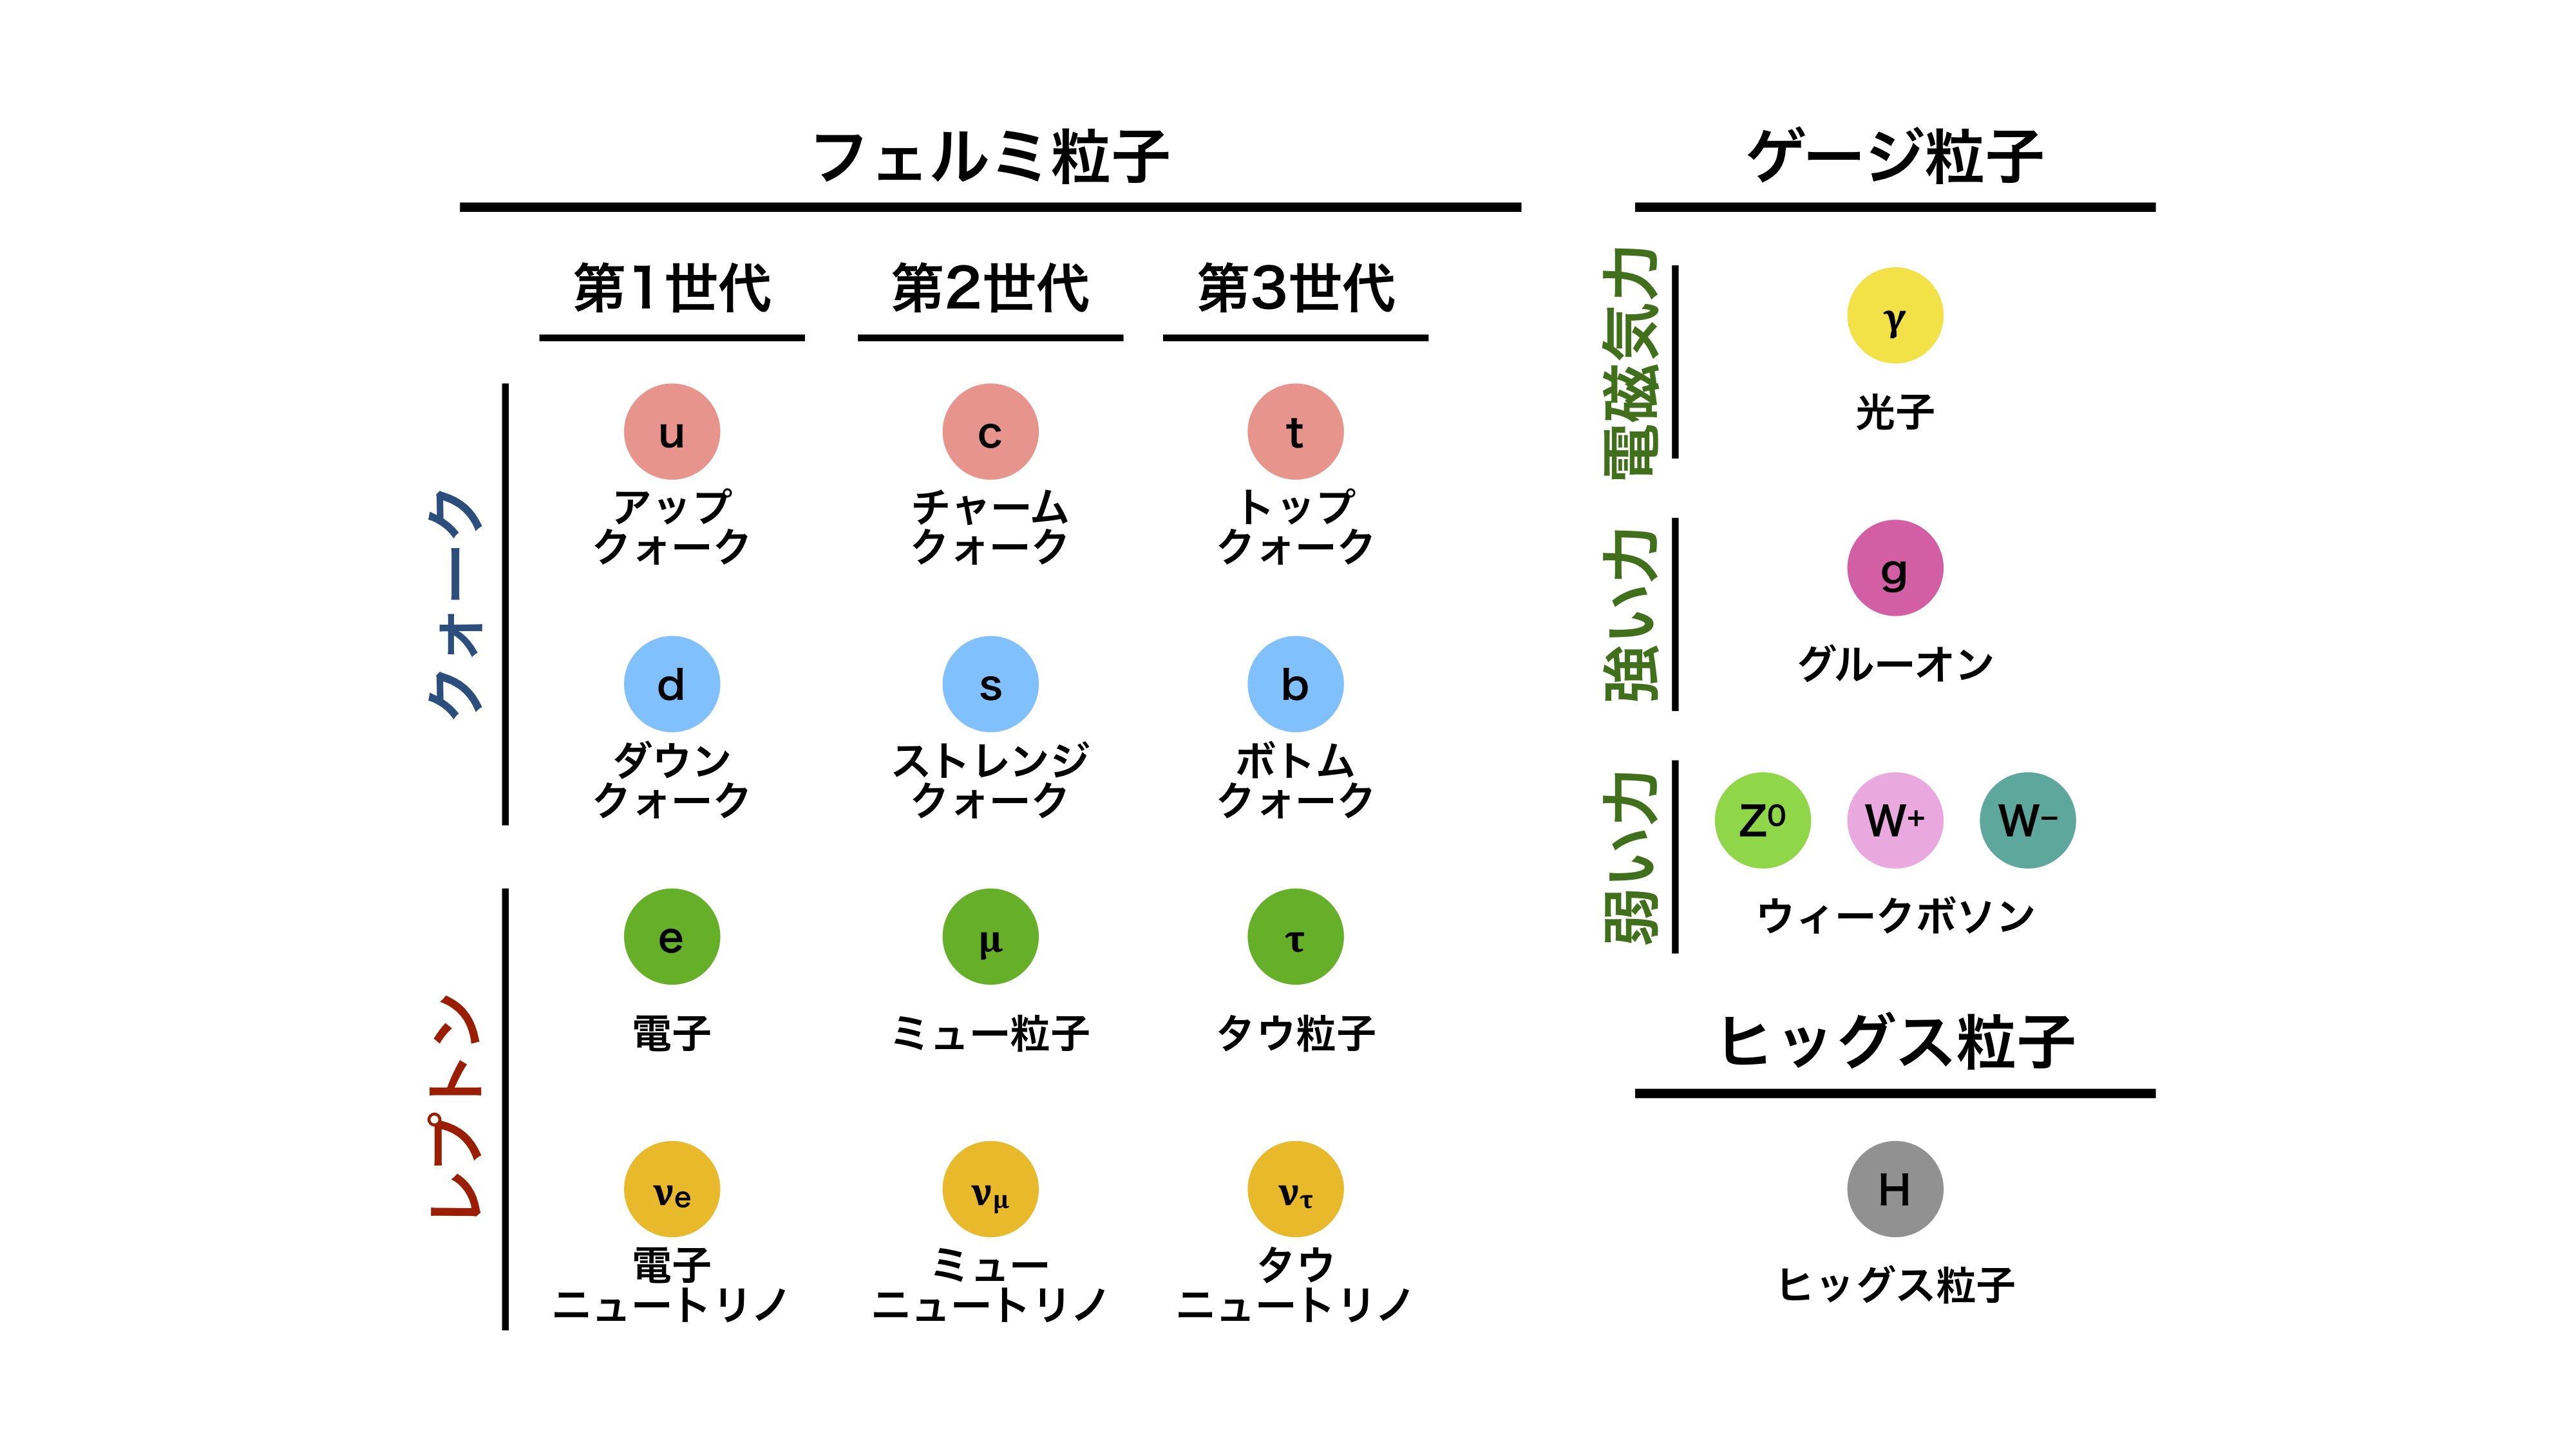
\includegraphics[width=0.9\textwidth]{Figure/1Introduction/1SMParticle.png}
 \caption{標準模型の素粒子}
 \label{1SMParticle}
\end{figure}

前述したように、標準模型は様々な実験で非常によく確かめられているが、ダークマターをはじめとするいくつかの物理現象を説明できておらず、現在は様々な実験によって、BSMの探索が行われている。
次節のILC計画はそのような試みの一つである。

%%%%%%%%%%%%%%%%%%%%%%%%%%%%%%%%%%%%%%%%%%%%%%%%%%%%%%%%%%%%%%%%%%%%%%%%%%%%%%%%%%%%%%%%%%%%%%%%%%%%%
\section{国際線形加速器 (ILC) 計画} \label{Intro:InternationalLinearColliderProject}

ILC計画とは、日本の東北にある北上山地に全長20.5kmの国際線形加速器 (ILC) を建設する計画である。 (図\ref{2InternationalLinearCollider})
ILC計画は国際共同研究であり、2013年に出版されたThe Technical Design Report (TDR)には2400人の研究者、48の国と392の研究機関と大学のグループが著名している。
このILC実現の為の技術開発はリニアコライダーコラボレーション (The Linear Collider Collaboration, LCC) によって推進され、LCCの活動は国際将来加速器委員会 (The International Committee for Future Accelerator, ICFA) の下、リニアコライダー国際推進委員会 (Linear Collider Board, LCB)によって監督されている。
現在ILC計画は準備段階へ向けて計画が進められており、日本のILC準備研究所 (ILC Pre-Lab) の為の準備としてICFAはILCの国際推進チーム (International Development Team, IDT) の設立を承認した。
今後はLCCやLCBに代わり、このILC国際推進チームがILC計画の推進を行なっていく予定である。
ILC計画の今後の流れは図\ref{3ILCProject}に示している。

\begin{figure}[h]
 \centering
  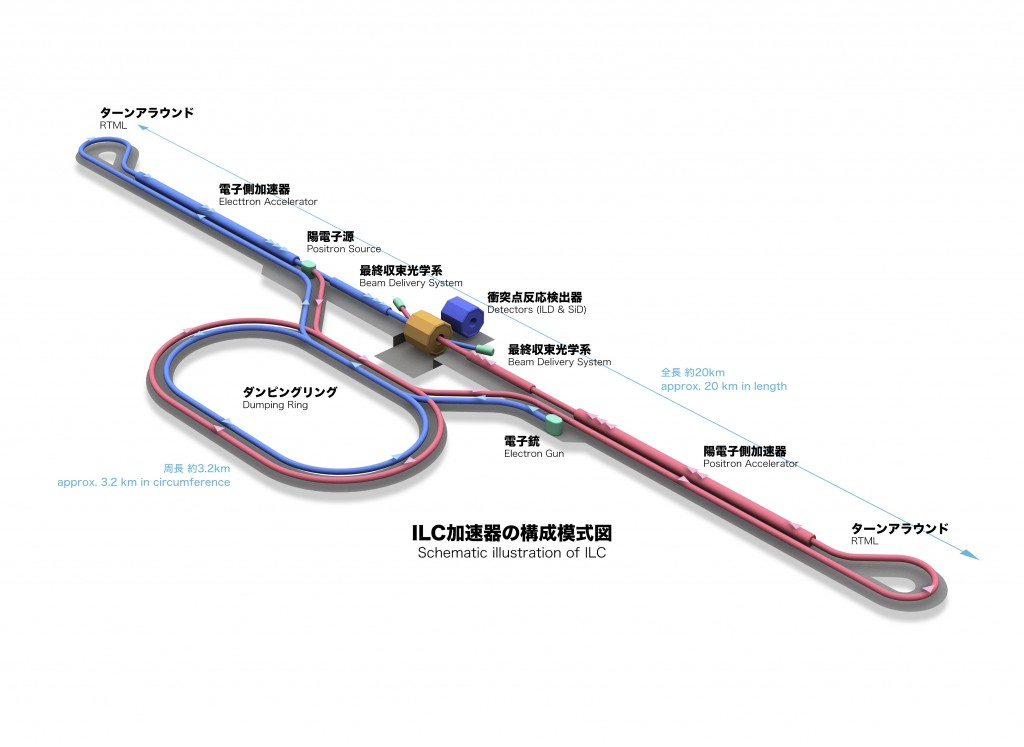
\includegraphics[width=0.9\textwidth]{Figure/1Introduction/2InternationalLinearCollider.jpg}
  \caption{国際線形加速器 (ILC) の外観\cite{ILCPHOTO}}
  \label{2InternationalLinearCollider}
\end{figure}


\begin{figure}[h]
 \centering
 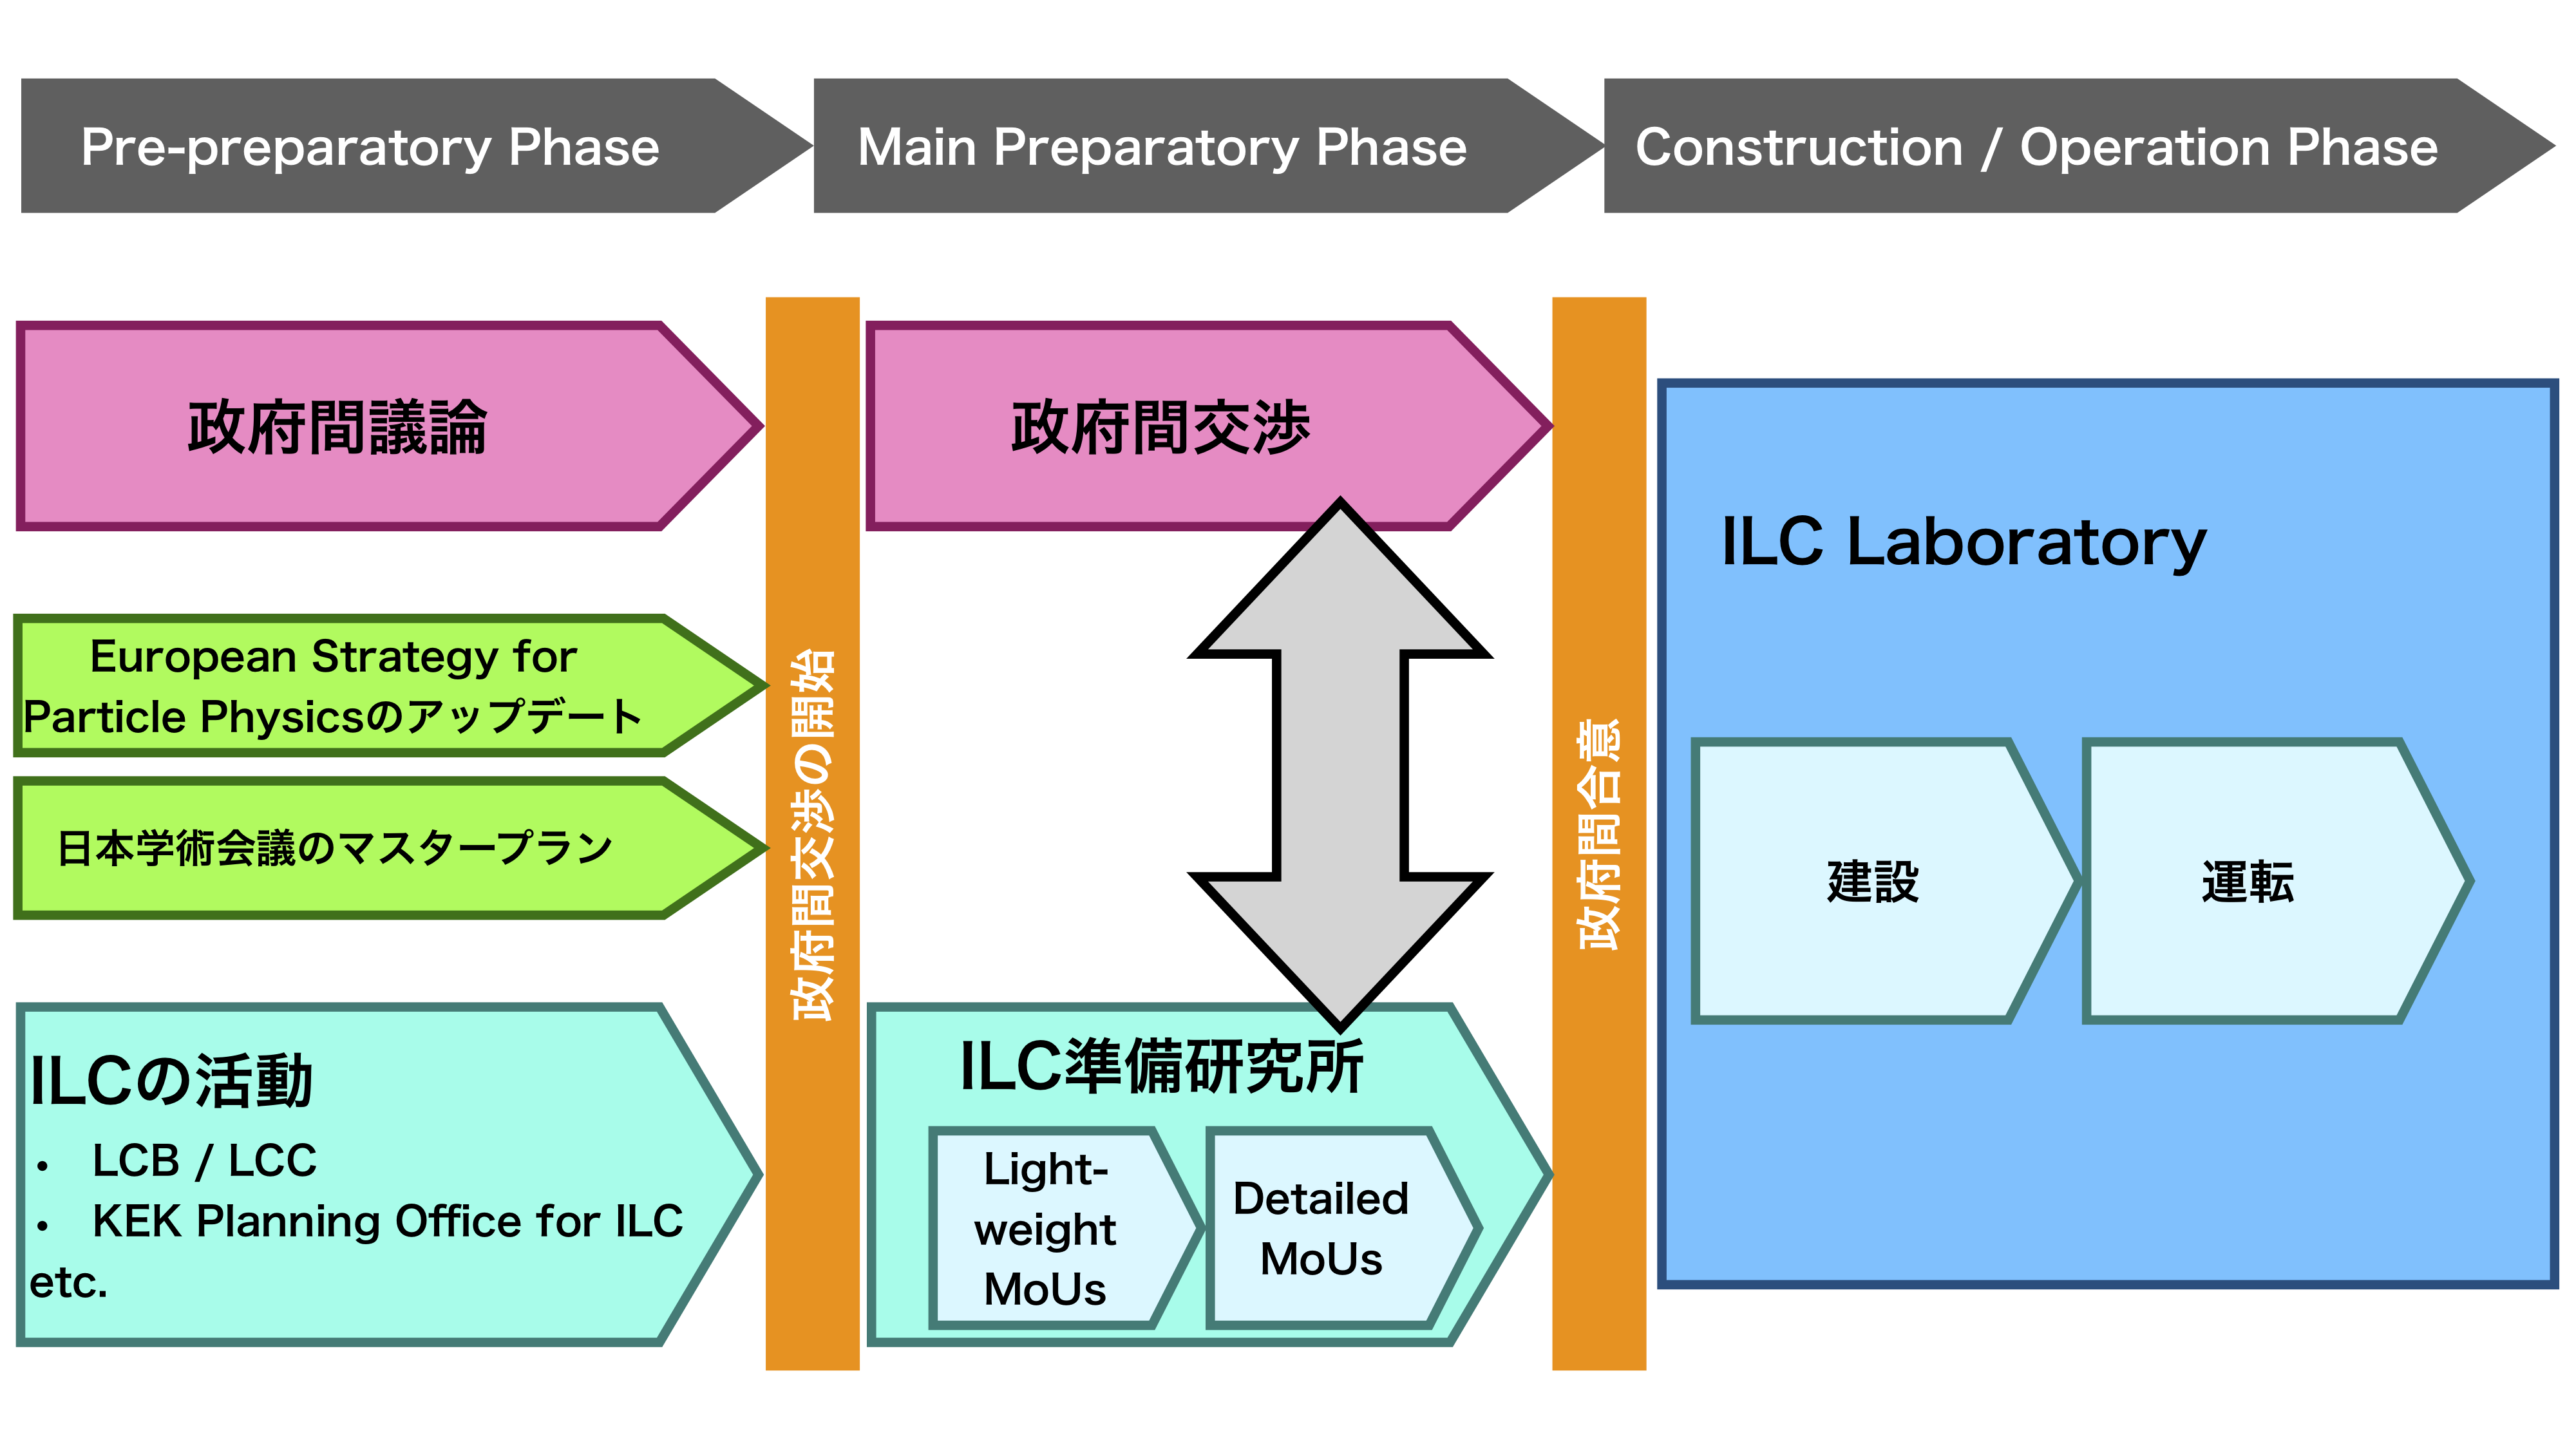
\includegraphics[width=0.9\textwidth]{Figure/1Introduction/3ILCProject.png}
 \caption{ILC計画の今後\cite{RecommendationsonILCProjectImplementation}}
 \label{3ILCProject}
\end{figure}

%%%%%%%%%%%%%%%%%%%%%%%%%%%%%%%%%%%%%%%%%%%%%%%%%%%%%%%%%%%%%%%%%%%%%%%%%%%%%%%%%%%%%%%%%%%%%%%%%%%%%
\section{ILCの物理} \label{Intro:PhysicsofILC}

ヒッグス粒子が2012年に欧州原子核研究機構(CERN)の大型ハドロン衝突型加速器(Large Hadron Collider, LHC)で発見されて以降、ヒッグス粒子の性質について、より詳細な調査が行われている。
ヒッグス粒子は標準模型の中で、電弱相互作用の対称性を破り、素粒子に質量を与える役割を担っており、また、質量に結合するという特徴を持っている。
このような振る舞いからヒッグス粒子の性質は標準模型によって詳細に決定される為、BSMによって標準模型との差異が生じた場合、ヒッグス粒子はその影響を受けると予想されている。
特にヒッグス粒子と他の粒子との結合定数の変化は、そのような仮定するBSMの模型の違いによって異なることが示唆されている。

ILCはこのヒッグス粒子の性質を詳細に調べる為のヒッグスファクトリーとしての役割を期待されている。
LHCが陽子-陽子衝突であるのに対し、ILCは電子-陽電子を衝突させる加速器である。
したがって、粒子反粒子の関係となっており、目的とする事象に対しエネルギーをより効率的に使うことができる。
また、電子-陽電子は陽子同士の衝突と異なり、背景事象が少ないという特徴を持っている。

ILCは$e^+e^- \to Zh$事象の反応断面積が最大となる重心系エネルギー$\sqrt{s}=250\ \mathrm{GeV}$での運転開始 (ILC250) を予定している。(図\ref{4eetoZH})
また、ILCには様々な物理目標を達成する為に多数のアップグレードオプションが存在し、重心系エネルギーについてはメインリニアックを延長することで$1\ \mathrm{TeV}$までの拡張が可能である。

\begin{figure}[h]
 \centering
 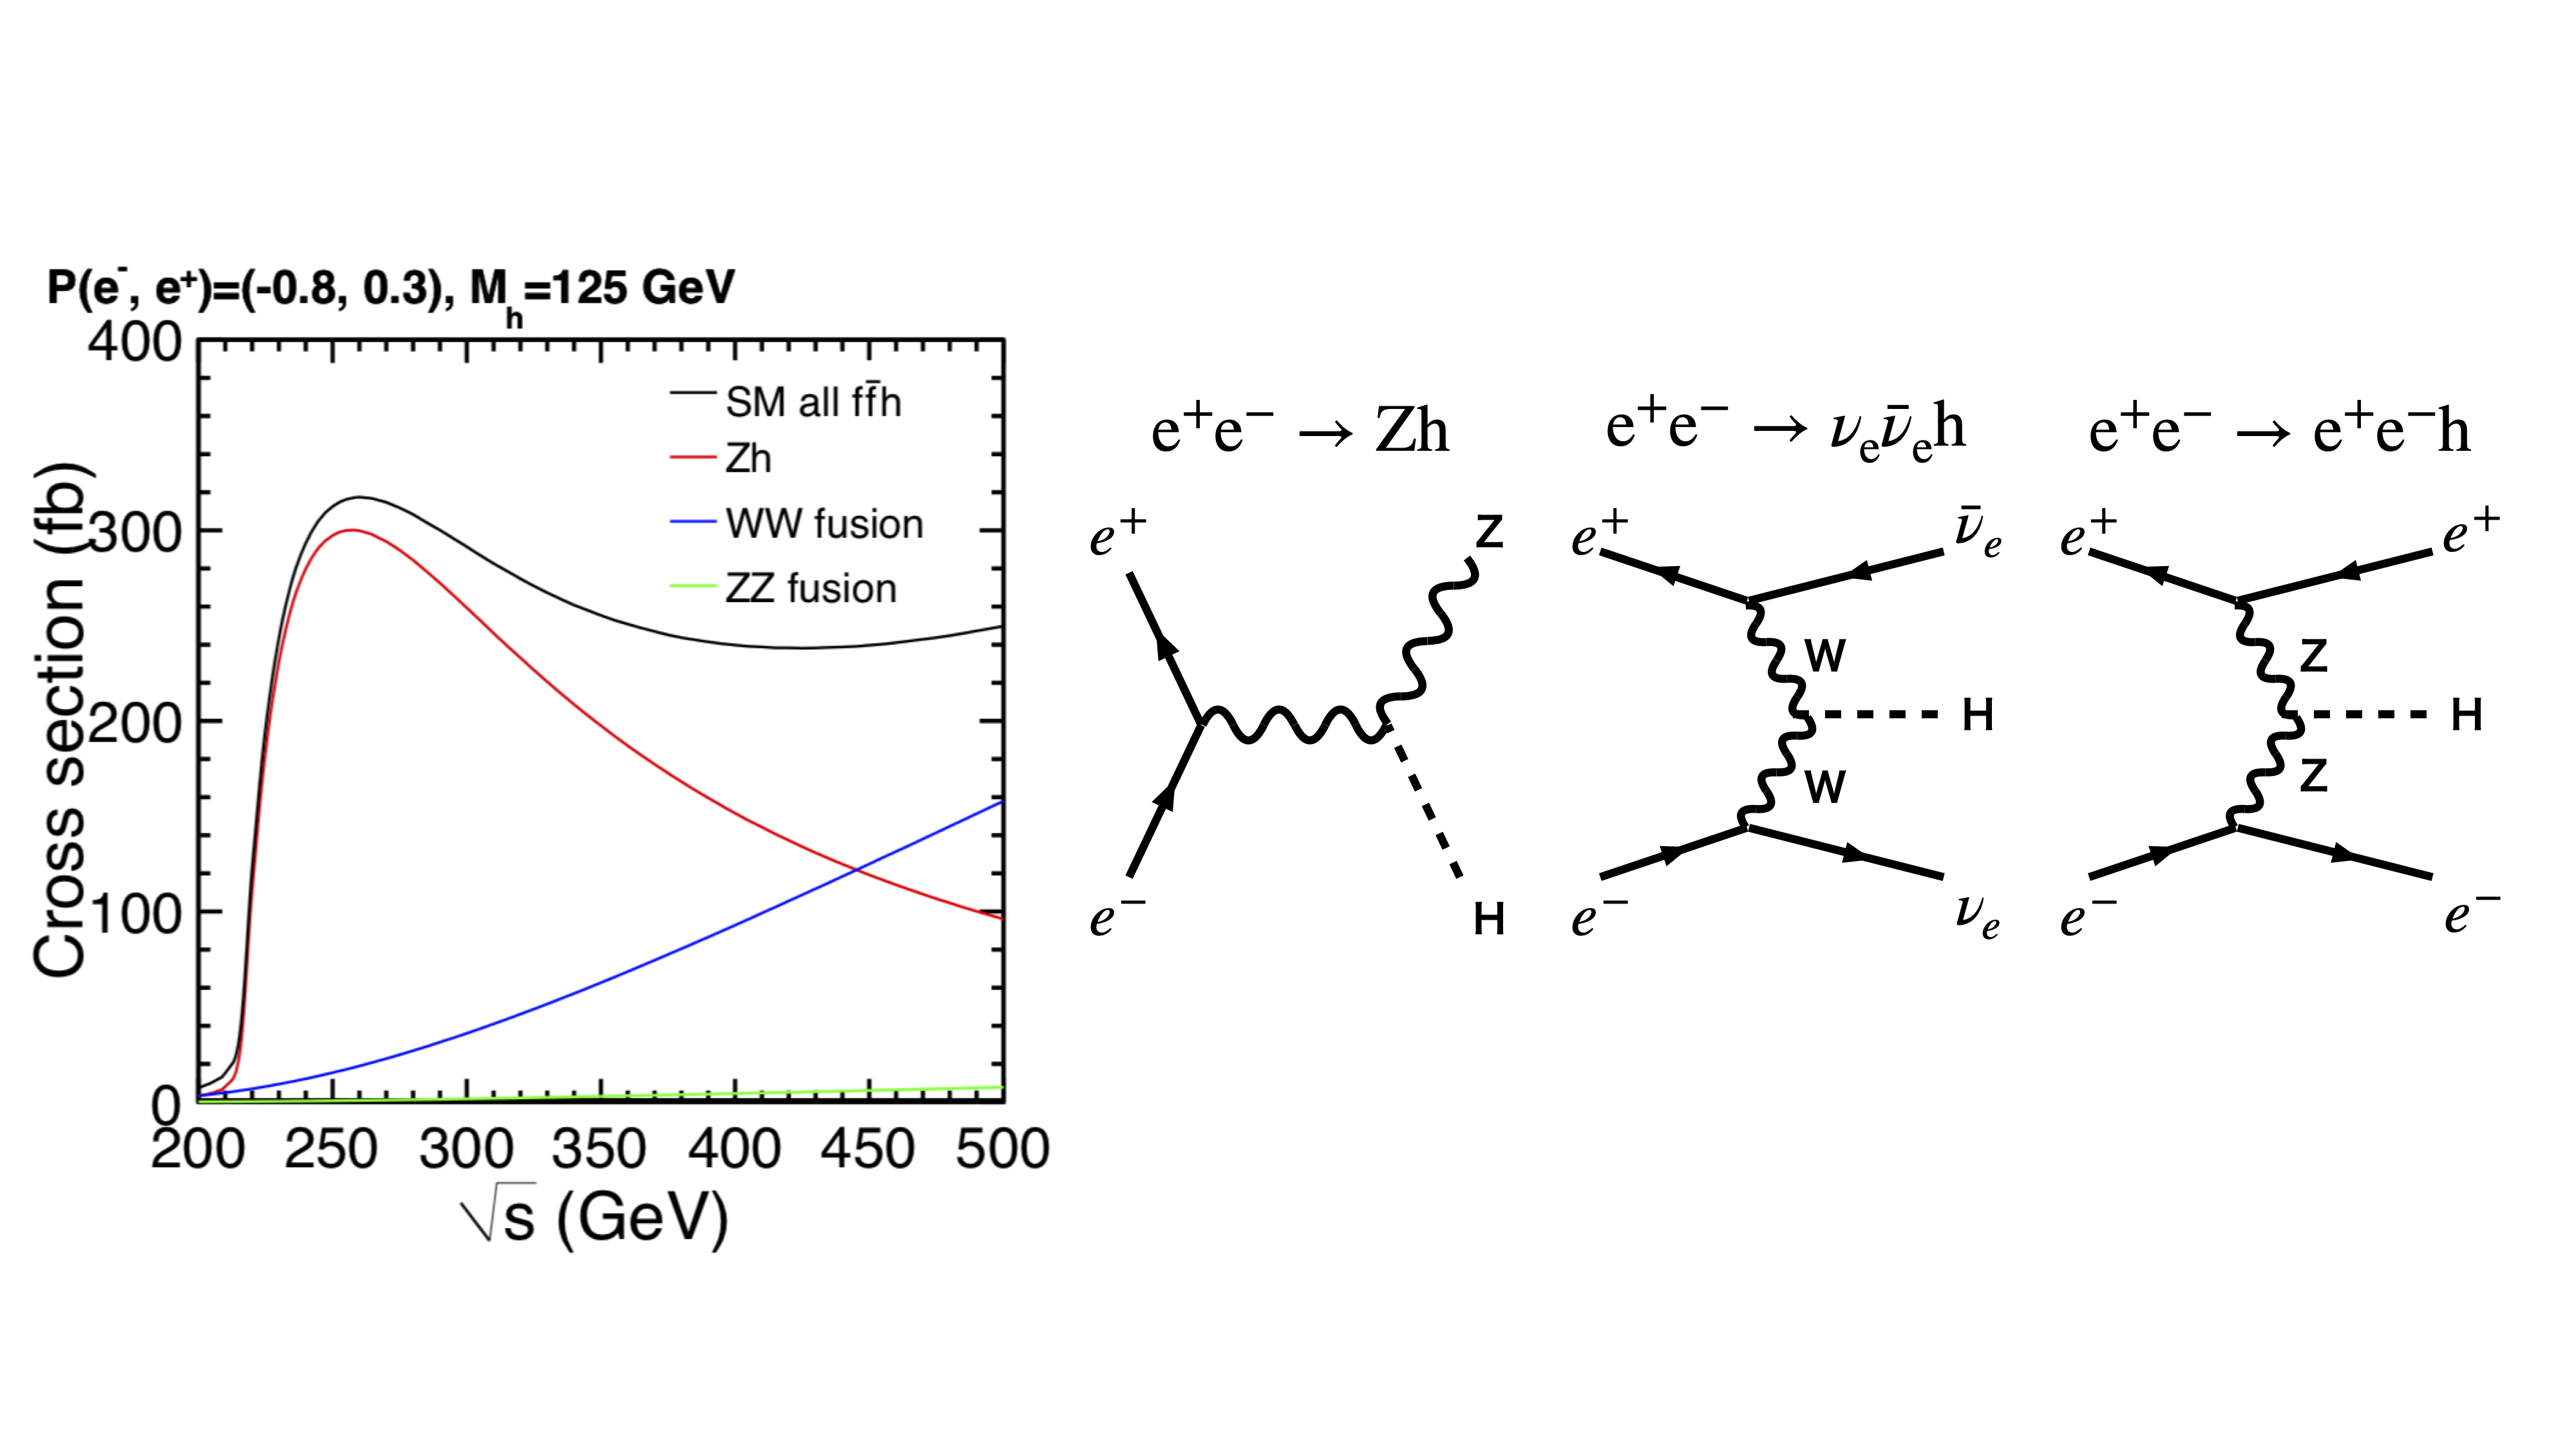
\includegraphics[width=0.7\textwidth]{Figure/1Introduction/4eetoZH.png}
 \caption{重心系エネルギーと断面積の関係\cite{TechnicalDesignReportPhysics}}
 % The International Linear Collider Technical Design Report - Volume 2: Physics Fig 2.7
 \label{4eetoZH}
\end{figure}

$e^+e^- \to Zh$事象は$Z$粒子の識別をすることによって、ヒッグスの崩壊モードに寄らず事象を選別できる (リコイル) という点で非常に重要である。
また、背景事象である$e^+e^- \to Z\gamma$や$e^+e^- \to ZZ$に関してもよく理解されており、電弱相互作用の計算によって$0.1\ \%$程度に抑えることができる。\cite{GlobalProject}
したがって、$e^+e^- \to Zh$事象の全断面積を得ることができ、絶対正規化されたヒッグス粒子の結合定数やヒッグス粒子のエキゾチック崩壊についての測定が可能である。

$e^+e^- \to Zh$事象での終状態の$Z$粒子は、レプトン対またはクォーク対に崩壊する。
レプトン対にはおよそ30\%程度の割合で崩壊し、クォーク対には残りの70\%程度の割合で崩壊する為、統計量を大きくするという点でクォーク対をより精度よく識別することは非常に重要である。
これらのクォーク対はエネルギー効率のために、それぞれ真空中でクォークの粒子反粒子対を生成・結合しハドロンとなる。
この過程で生成されたクォークも同様にハドロンを形成するため、初めのクォーク対のそれぞれの進行方向には多数のハドロン粒子が生成されることとなる。
これをジェットといい、$Z$粒子を始めとする様々な粒子のクォーク対への崩壊は、このジェットを用いて識別される。
そのようなジェットの再構成については、\ref{Intro:SoftERILC:JetReconstruction}項にて説明する。

%%%%%%%%%%%%%%%%%%%%%%%%%%%%%%%%%%%%%%%%%%%%%%%%%%%%%%%%%%%%%%%%%%%%%%%%%%%%%%%%%%%%%%%%%%%%%%%%%%%%%
\section{ILCの検出器 -International Large Detector (ILD)-} \label{Intro:InternationalLargeDetector}

ILCでは二つの検出器が検討されており、ILD(図\ref{5-1InternationalLargeDetector})はその一つである。
ILDはヒッグス粒子や電弱相互作用の物理からの要求値を満たすように設計され、また後述するParticle Flow (\ref{Intro:SoftERILC:ParticleReconstruction}項) によって最適化されている。
また、様々なサブディテクターによって構成され、ビームの衝突点 (図\ref{5-2InternationalLargeDetector}の右下) を包む様に内側から順に、Vertex Detector (VTX)、Silicon Internal Tracker (SIT)、Time Projection Chamber (TPC)、Electromagnetic Calorimeter (ECAL)、Hadron Calorimeter (HCAL)、Iron Yoke (Muon が並んでいる。
HCALとIron Yokeの間にはSolenoid Coilがあり、$3.5 \mathrm{T}$の磁場をかけている。
VTXやSIT、TPCを用いて荷電粒子の飛跡を測定し、ECALによって電子や光子などの粒子のエネルギーを、HCALによってハドロン粒子のエネルギーを測定する。
衝突点の前方方向には、Forward Tracking Detector (FTD)、Luminosity Calorimeter (LumiCAL)、LHCAL、Beam Calorimeter (BeamCAL)が並んでいる。
それぞれの技術的な詳細については表\ref{ILDSubdetectorParametersBarrel}、\ref{ILDSubdetectorParametersEndCap}にまとめる。

\begin{figure}[h]
 \centering
 \begin{minipage}{0.47\textwidth}
  \centering
  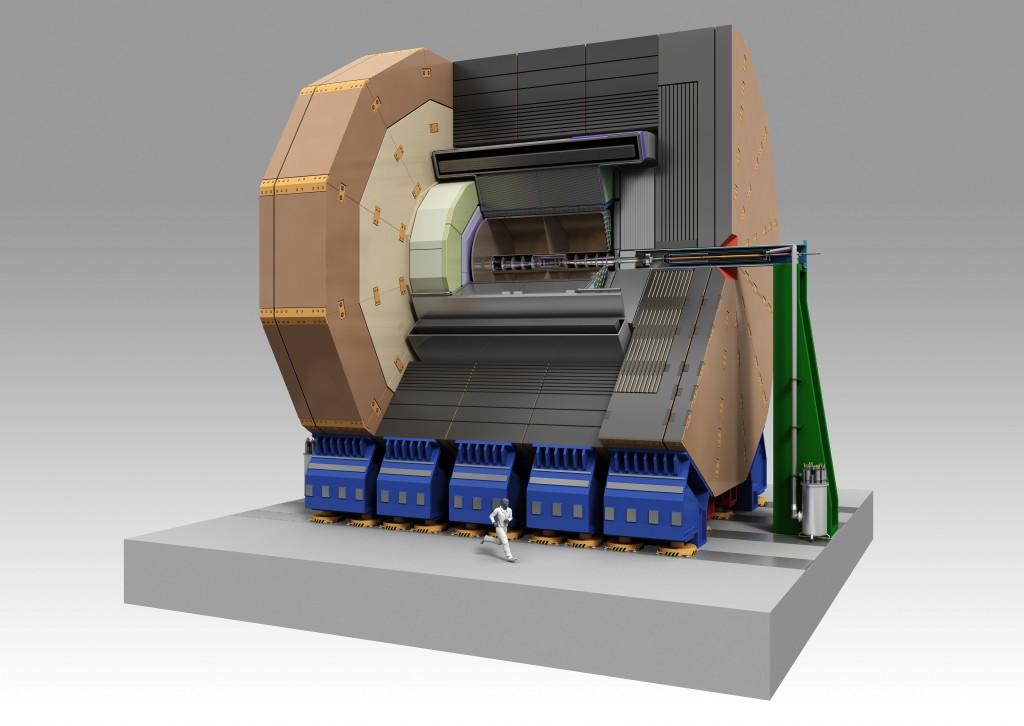
\includegraphics[width=1\textwidth]{Figure/1Introduction/5-1InternationalLargeDetector.jpg}
  \caption{外観\cite{ILCPHOTO}}
  \label{5-1InternationalLargeDetector}
 \end{minipage}
 \begin{minipage}{0.47\textwidth}
   \centering
   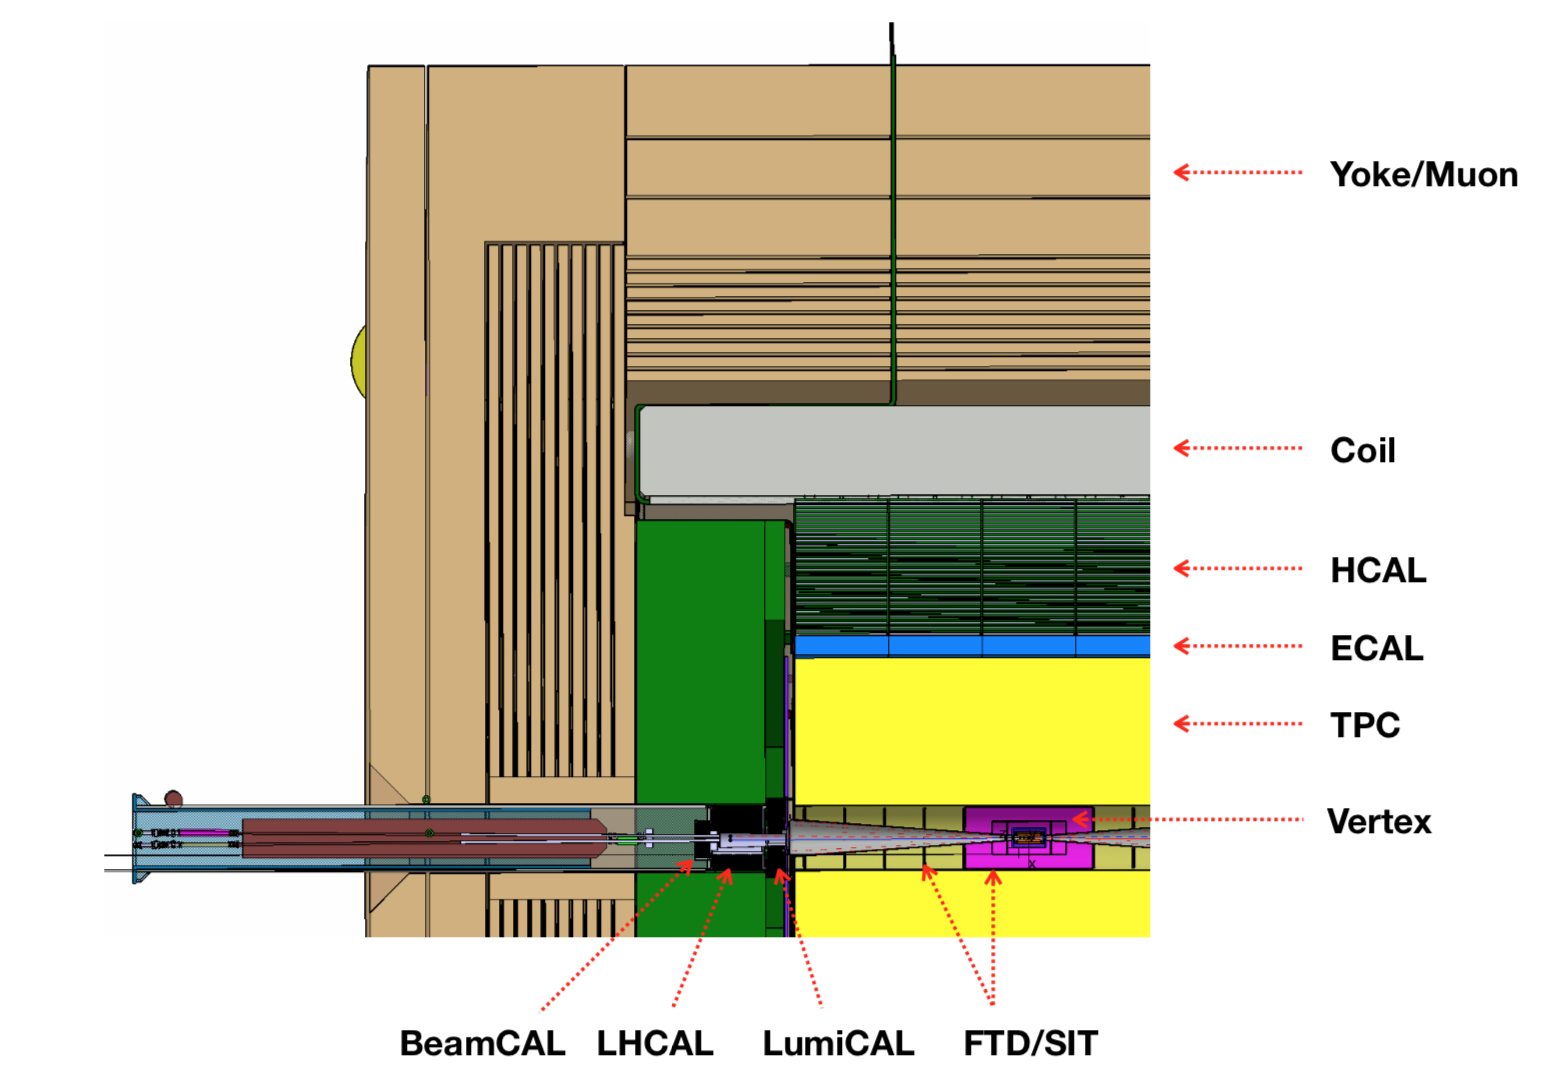
\includegraphics[width=1\textwidth]{Figure/1Introduction/5-2InternationalLargeDetector.png}
   \caption{縦断面\cite{InterimDesignReport}}
   \label{5-2InternationalLargeDetector}
    % INTERIM DESIGN REPORT Figure 5.1
 \end{minipage}
 \caption{International Large Detector (ILD)}
\end{figure}

\begin{table}[htb]
  \small
  \begin{tabular}{l c c c l} \hline
     & $r_{in} \mathrm{[mm]}$ & $r_{out} \mathrm{[mm]}$ & $z_{max} \mathrm{[mm]}$ & 要素技術\\ \hline \hline
    VTX & 16 & 60 & 125 & シリコンピクセルセンサー\\
    SIT & 153 & 303 & 644 & シリコンピクセルセンサー\\
    TPC & 329 & 1770 & 2350 & マイクロパターンガス検出器\\
    SET & 1773 & 1776 & 2300 & シリコンストリップセンサー\\ \hline
    ECAL & 1805 & 2028 & 2350 & 吸収層 : タングステン\\
    &&&& センサー : シリコン/シンチレーター\\
    HCAL & 2058 & 3345 & 2350 & 吸収層 : スチール\\
    &&&& センサー : シンチレーター/RPCガス\\ \hline
    Coil & 3425 & 4175 & 3872\\
    Muon & 4450 & 7755 & 4047 & センサー : シンチレーター\\ \hline
  \end{tabular}
  \caption{ILDサブディテクターの詳細なパラメータ (バレル) \cite{InterimDesignReport}}
  \label{ILDSubdetectorParametersBarrel}
\end{table}

\begin{table}[htb]
 \small
  \begin{tabular}{l c c c c l} \hline
     & $z_{min} \mathrm{[mm]}$ & $z_{max} \mathrm{[mm]}$ & $r_{in} \mathrm{[mm]}$ & $r_{out} \mathrm{[mm]}$ & 要素技術\\ \hline \hline
    FTD & 220 & 371 & & 153 & シリコンピクセルセンサー\\
            & 645 & 2212 & & 300 & シリコンストリップセンサー\\ \hline
    ECAL & 2411 & 2635 & 250 & 2096 & 吸収層 : タングステン\\
    &&&&& センサー : シリコン/シンチレーター\\
    HCAL & 2650 & 3937 & 350 & 3226 & 吸収層 : スチール\\
    &&&&& センサー : シンチレーター/RPCガス\\
    Muon & 4072 & 6712 & 350 & 7716 & センサー : シンチレーター\\ \hline
    BeamCAL & 3115 & 3315 & 18 & 140 & 吸収層 : タングステン\\
    &&&&& GaAs読み出し \\
    LumiCAL & 2412 & 2541 & 84 & 194 & 吸収層 : タングステン\\
    &&&&& センサー : シリコン\\
    LHCAL & 2680 & 3160 & 130 & 315 &吸収層 : タングステン\\ \hline
  \end{tabular}
  \caption{ILDサブディテクターの詳細なパラメータ (エンドキャップ) \cite{InterimDesignReport}}
  \label{ILDSubdetectorParametersEndCap}
\end{table}

%%%%%%%%%%%%%%%%%%%%%%%%%%%%%%%%%%%%%%%%%%%%%%%%%%%%%%%%%%%%%%%%%%%%%%%%%%%%%%%%%%%%%%%%%%%%%%%%%%%%%
\section{ILCのソフトウェアと事象再構成} \label{Intro:SoftwareandEventReconstructionofILC}

ここではILCで使用されるソフトウェアと事象再構成について述べる。
ILCのソフトウェアはiLCSoft\cite{iLCSoft}と呼ばれるソフトウェアエコシステムにまとめられている。
ILCにおける事象再構成は、トラッキングやParticle Flowといった\ref{Intro:SoftERILC:ParticleReconstruction}. 粒子の再構成と、更にそれらによって再構成された粒子を使いジェットを再構成する\ref{Intro:SoftERILC:JetReconstruction}. ジェットの再構成に分けられる。
ILCではジェットの再構成は崩壊点検出、ジェットクラスタリング、フレーバータギングという行程に分けられる。
これらジェットの再構成はiLCSoft内のLCFIPlus\cite{LCFIPlus}によって行われている。

%%%%%%%%%%%%%%%%%%%%%%%%%%%%%%%%%%%%%%%%%%%%%%%%%%%%%%%%%%%%%%%%%%%%%%%%
\subsection{ソフトウェア} \label{Intro:SoftERILC:Software}

書く事\\
LCIO・Marlin・DD4hep\\


%%%%%%%%%%%%%%%%%%%%%%%%%%%%%%%%%%%%%%%%%%%%%%%%%%%%%%%%%%%%%%%%%%%%%%%%
\subsection{飛跡の再構成} \label{Intro:SoftERILC:ParticleReconstruction}

書く事\\
トラッキング・Particle Flow\\

%%%%%%%%%%%%%%%%%%%%%%%%%%%%%%%%%%%%%%%%%%%%%%%%%%%%%%%%%%%%%%%%%%%%%%%%
\subsection{ジェットの再構成} \label{Intro:SoftERILC:JetReconstruction}

書く事\\
トラッキング・Particle Flowを経て再構成された粒子の飛跡を用いて、ジェットの再構成が行われる。
粒子が飛んでーーーーprimary vertexとsecondary vertex (崩壊点) を形成する\\
secondary vertexはジェットの種であり、これを検出するアルゴリズムを崩壊点検出といい、その様にして検出されたsecondary vertexを用いて、中性電荷を合わせた飛跡について、どのジェットに属するかクラスタリングを行うアルゴリズムをジェットクラスタリングという。
また、secondary vertexによってーーーーをフレーバータギングという。
以上がジェットの再構成である。
ここでは、LCFIPlus\cite{LCFIPluspaper}でのジェット再構成手法についてまとめる。

まず、Primary Vertex

次に、Secondary Vertex

ジェットクラスタリング・Durham

フレーバータギング・Boosted Decision Trees (BDTs)

%%%%%%%%%%%%%%%%%%%%%%%%%%%%%%%%%%%%%%%%%%%%%%%%%%%%%%%%%%%%%%%%%%%%%%%%%%%%%%%%%%%%%%%%%%%%%%%%%%%%%
\section{本研究の目的} \label{Intro:Purpose}

\begin{figure}[h]
 \centering
 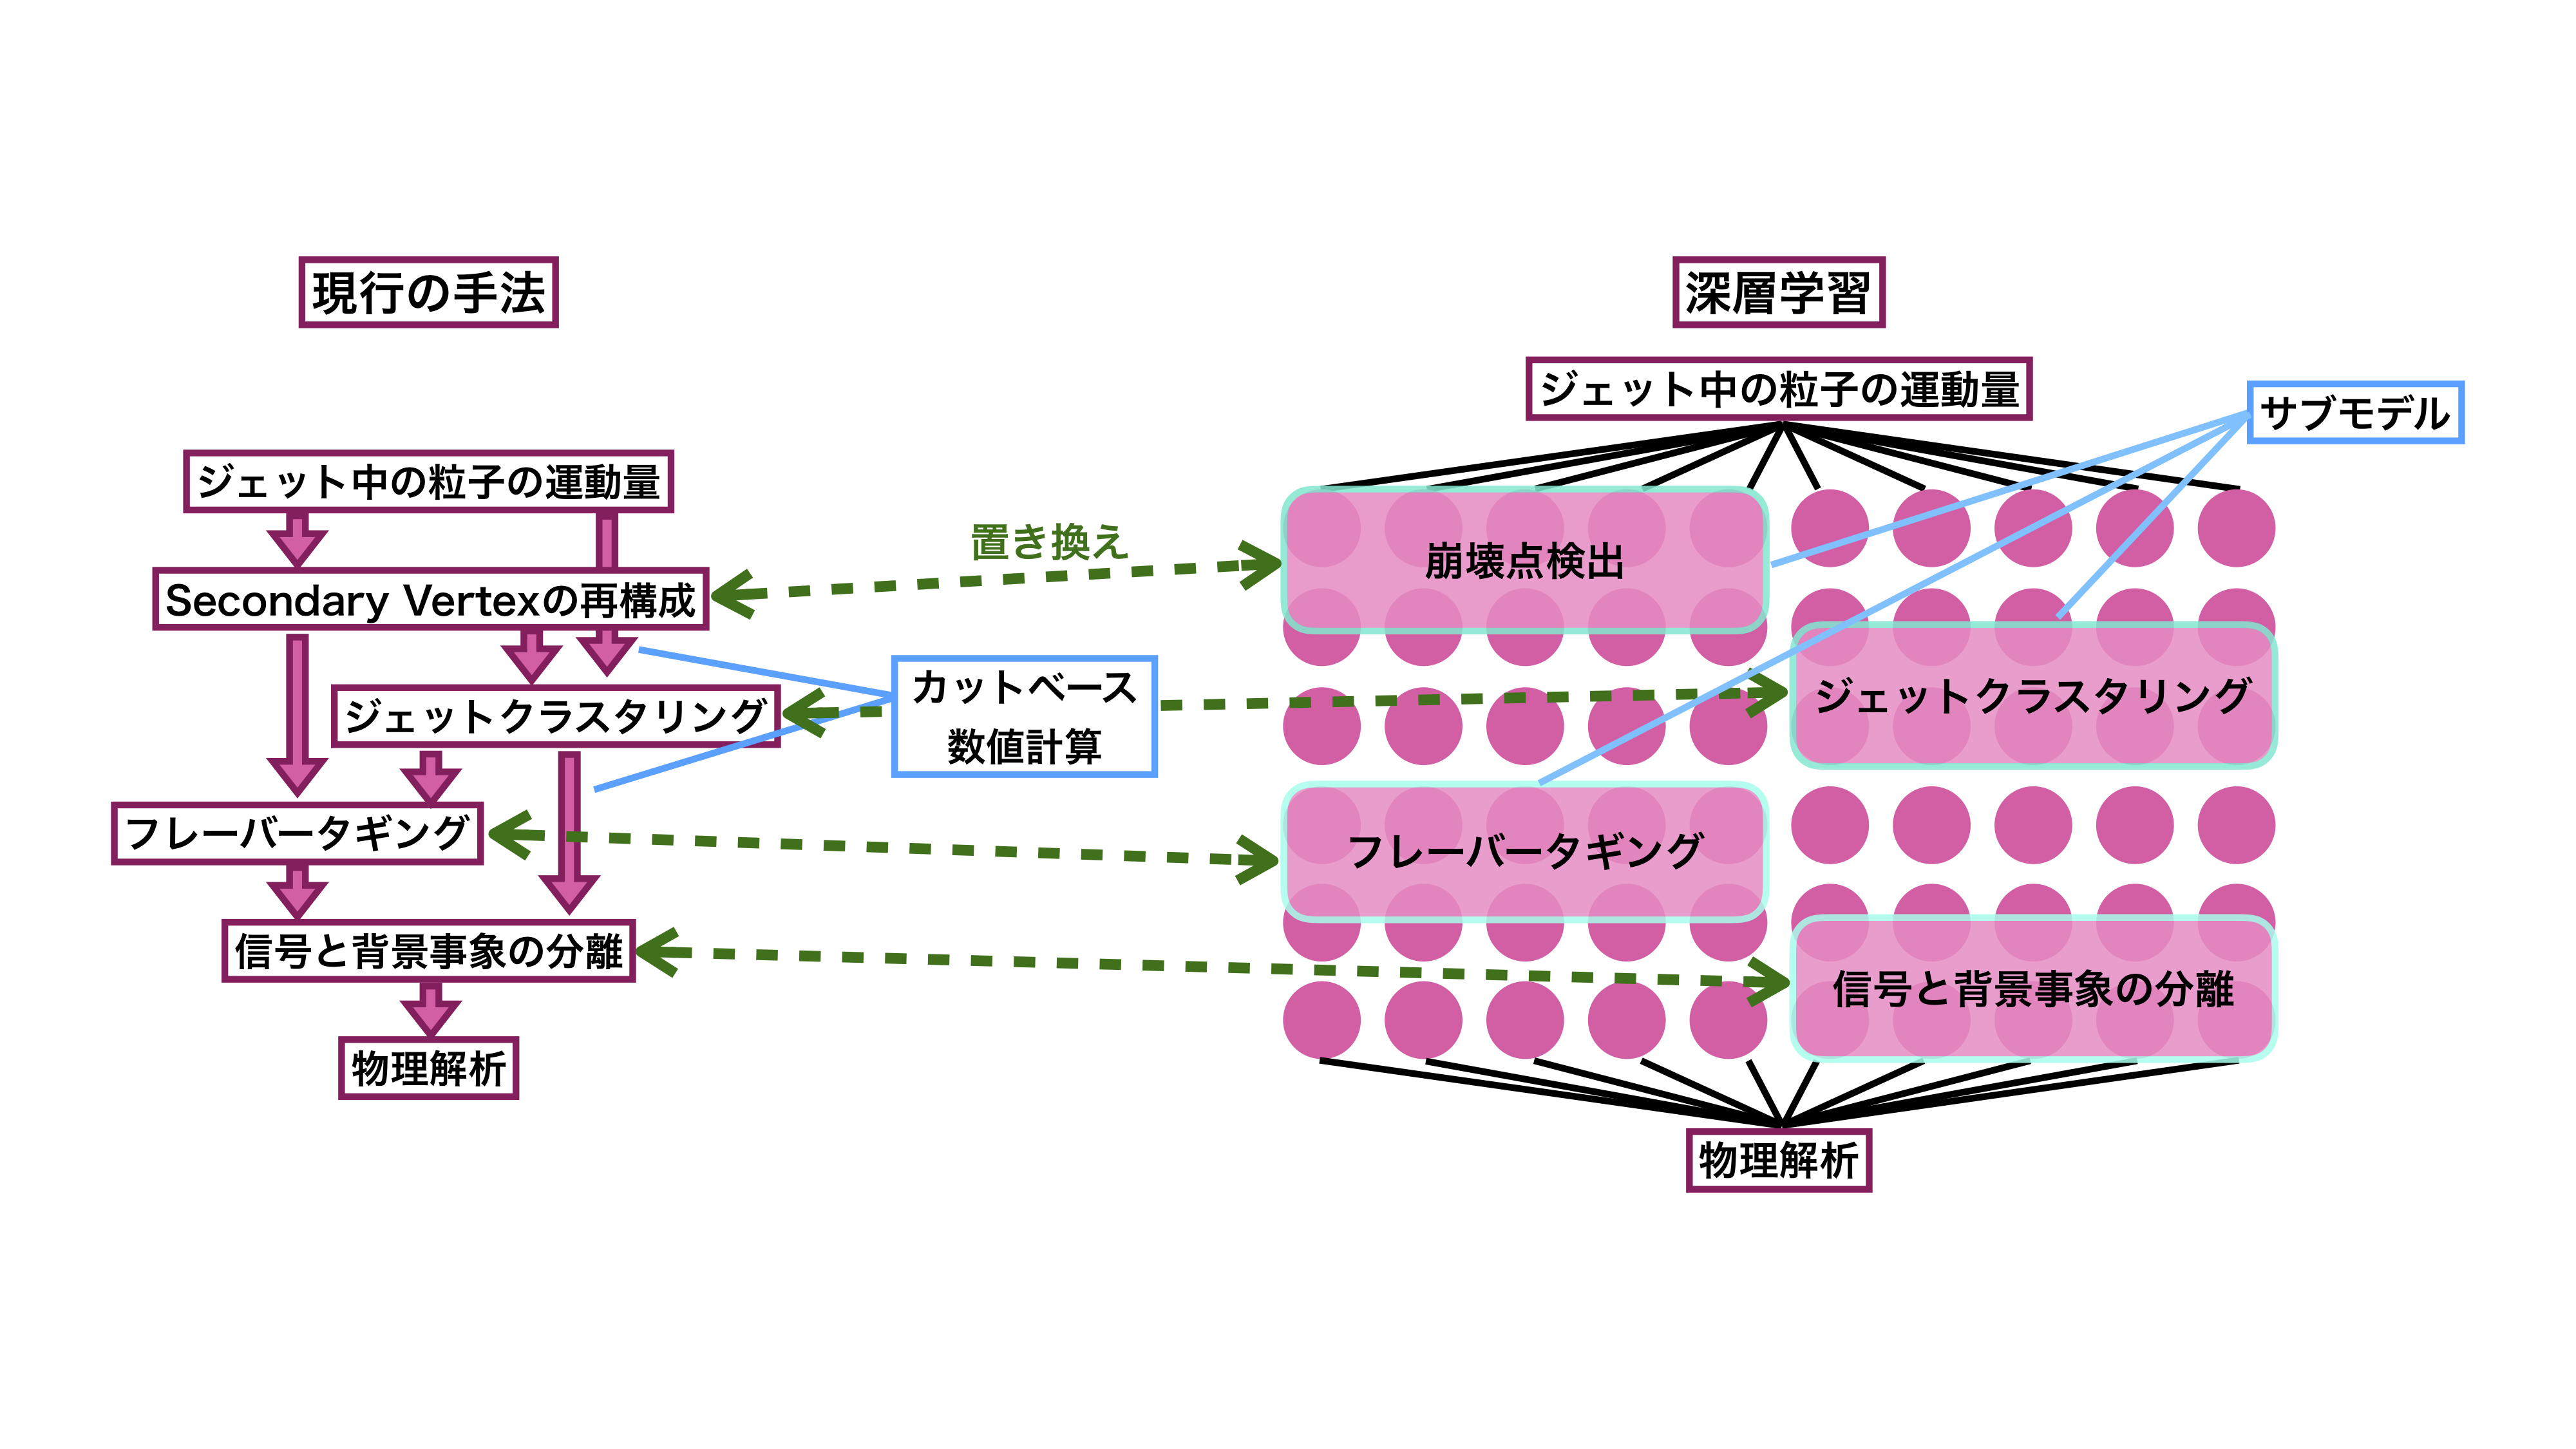
\includegraphics[width=1.0\textwidth]{Figure/1Introduction/6JetReconstructionwithDeepLearning.png}
 \caption{深層学習によるジェットの再構成}
 \label{6JetReconstructionwithDeepLearning}
\end{figure}


















% !TEX root = ../MasterThesis_goto_v1.tex

%%%%%%%%%%%%%%%%%%%%%%%%%%%%%%%%%%%%%%%%%%%%%%%%%%%%%%%%%%%%%%%%%%%%%%%%%%%%%%%%%%%%%%%%%%%%%%%%%%%%%
\chapter{深層学習} \label{chap:DeepLearning}

本章では, 深層学習 (Deep Learning, DL) について述べる。

まず深層学習の導入として, \ref{DL:MachineandDeepLearning}節で機械学習 (Machine Learning, ML) と深層学習の概要について簡単に紹介する。

次に\ref{DL:Perceptron}節では, 深層学習を理解する上で前提となるパーセプトロン (Perceptron) というネットワークを解説する。
パーセプトロンは, 後述するニューラルネットワークの先駆けとなる技術である。

\ref{DL:NeuralNetwork}節では, 深層学習の基礎技術であるニューラルネットワーク (Neural Network, NN) を導入する。
主に, \ref{DL:NN:StructureofNN}項でニューラルネットワークを構築するために必要な計算手順について, \ref{DL:NN:TrainingofNN}項でニューラルネットワークの学習に関して重要な技術要素についてそれぞれ説明する。

深層学習は, \ref{DL:NeuralNetwork}節までの基盤的な技術を使用するだけでも様々な問題に対応できるが, 扱うデータや問題の性質によって, 更に応用的な使い方が求められる。
本研究ではそのような応用技術を幾つか用いてネットワークの作成を行なっている。
その為, \ref{DL:RecurrentNeuralNetwork}節や\ref{DL:Attention}節ではそのような深層学習の応用技術の解説を行う。

\ref{DL:RecurrentNeuralNetwork}節では, 系列データを取り扱うためのリカレントニューラルネットワーク (Recurrent Neural Network, RNN) を導入する。
\ref{DL:Attention}節では, 近年注目されている注意機構 (Attention) と呼ばれる技術について説明する。

最後に\ref{DL:HyperParameter}節にて, ニューラルネットワークが持つハイパーパラメータについてまとめる。

本章の作成にあたり, 参考文献\cite{ZeroDeepLearning1, ZeroDeepLearning2, PythonMLPrograming}を使用した。

%%%%%%%%%%%%%%%%%%%%%%%%%%%%%%%%%%%%%%%%%%%%%%%%%%%%%%%%%%%%%%%%%%%%%%%%%%%%%%%%%%%%%%%%%%%%%%%%%%%%%
\section{機械学習と深層学習} \label{DL:MachineandDeepLearning}

深層学習とは, 機械学習の技術の一つである。
本節ではまず, この機械学習について簡単に説明し, その後, 機械学習における深層学習の位置付けを述べる。

機械学習とは, データに現れるパターンや統計情報を計算機 (学習器) に「学習」させることによって, 逐一プログラミングをすることなく未知の問題に対応させる為の技術である。
これは人間の持つ知性を機械に実現する, 人工知能 (Artificial Intelligence, AI) に関する研究の一分野であると言える。
このような研究は, $1956$年のダートマス会議\cite{Dartmouth}から始まり, 現在は第三期のAIブームと言われている。
機械学習は, 機械 (計算機) が独自に未知の問題を解く為の技術や手法の総称であるが, 問題に対するアプローチの仕方によって, 教師あり学習, 教師なし学習, 強化学習などに分類することができる(図\ref{1MachineLearning})。

\begin{itemize}
  \item 教師あり学習\\
  教師あり学習とは, 訓練データ (Training data) と呼ばれる正解がラベル付けされたデータを用い, 学習器の出力を正解に近付けるように学習器を更新していく手法である。
  主にクラス分類を行う分類問題や, 連続値を予測する回帰問題などの問題を解くことができる。
  具体的な例としてサポートベクターマシン (Support Vector Machine, SVM\cite{PatternRecognitionUsingGeneralizedPortraitMethod,TrainingAlgorithmforOptimalMarginClassifiers})や決定木などが挙げられる。
  \item 教師なし学習\\
  教師なし学習とは, 訓練データを用いず, データの持つ数学モデルや構造を抽出する技術である。
  主にクラスタリングや次元圧縮などに使用され, 代表的な手法は, k平均法や主成分分析などである。
  \item 強化学習\\
  強化学習とは, 環境とのやり取りから報酬を受け取り, エージェントを構築していく手法である。
  学習は報酬を最大化するように進み, 教師あり学習の一分野のようにみなす事も出来るが, 強化学習は一連の行動に対しての報酬を考慮する点で異なる。
  強化学習は様々な分野で使用されているが, 主に長期的な戦略が必要となるゲームなどの領域で用いられている。
\end{itemize}

\begin{figure}[htbp]
 \centering
 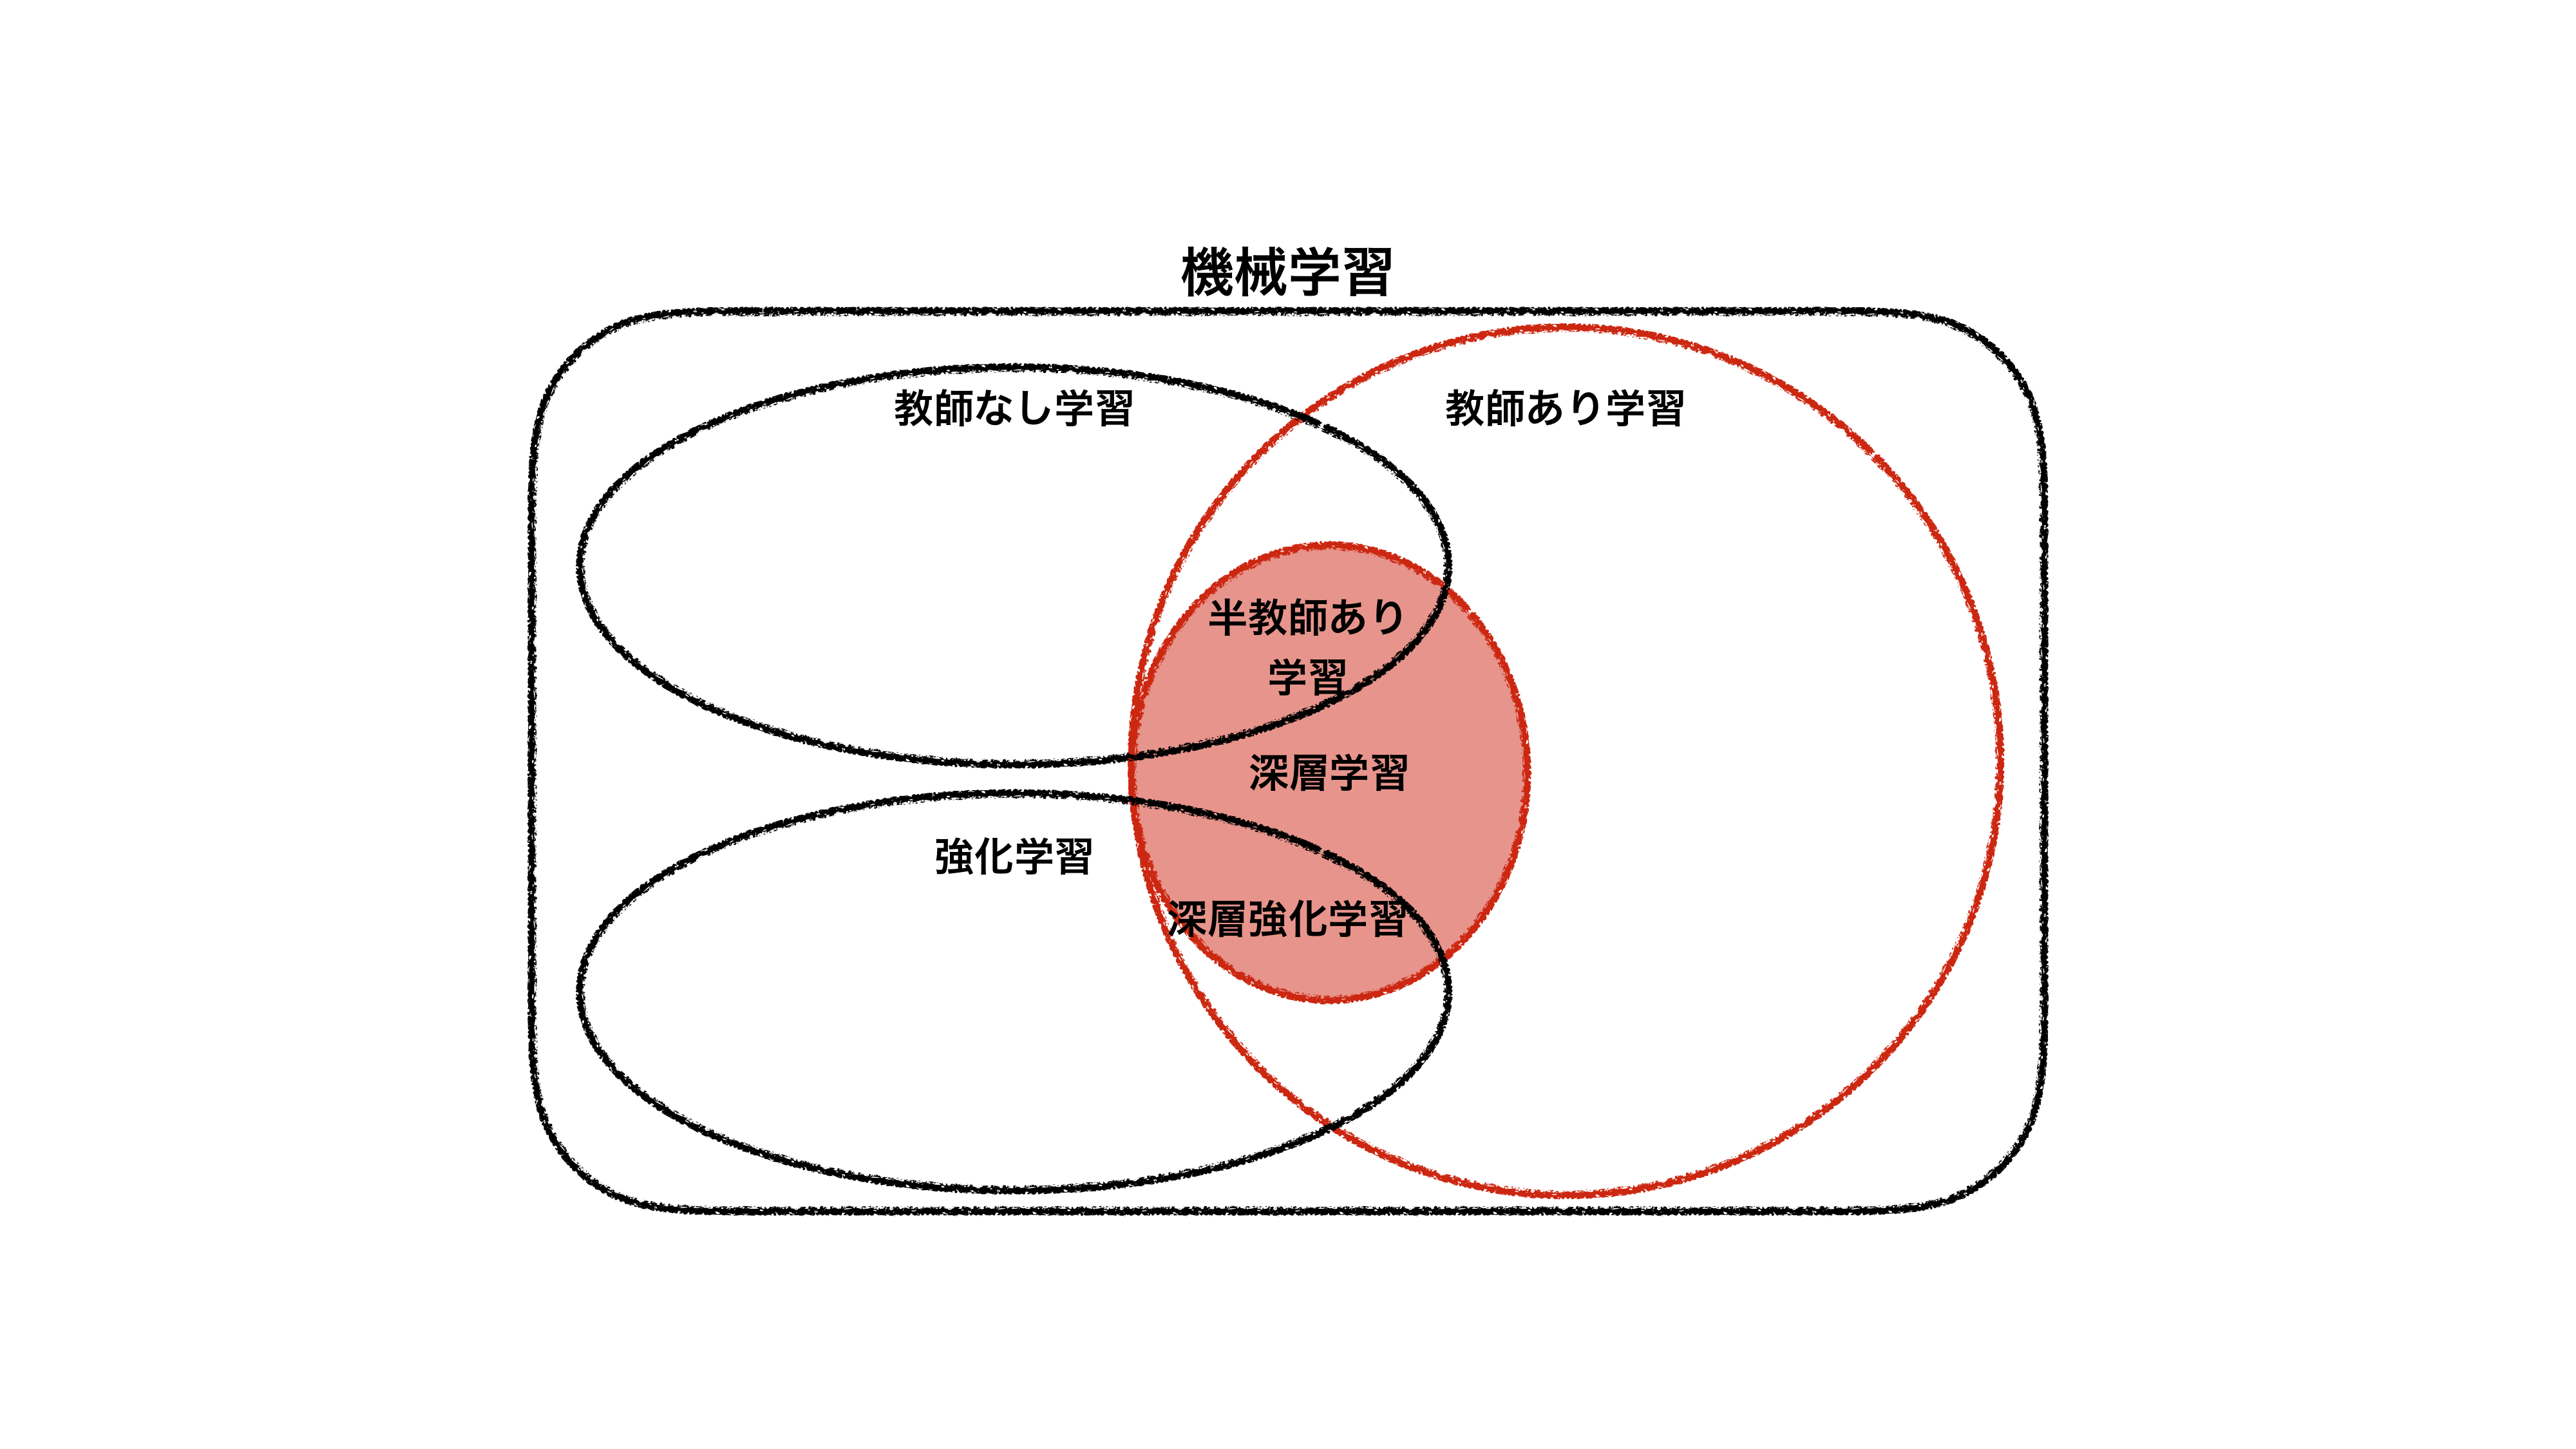
\includegraphics[trim = 0 100 0 50, width=0.9\textwidth, clip]{Figure/2DeepLearning/1MachineLearning.png}
 \caption[機械学習の中の深層学習の位置付け]{機械学習の中の深層学習の位置付け。深層学習は基本的に教師あり学習であるが, 半教師あり学習分類やクラスタリングなど応用的な研究が行われている。}
 \label{1MachineLearning}
\end{figure}

深層学習は, このような機械学習の中で, 基本的には, 回帰問題や分類問題などを解く教師あり学習に分類される。
しかし近年では, 半教師あり学習やディープクラスタリング, 深層強化学習といった様々な技術的応用が提案されている。
次節以降では, この深層学習の基盤技術について紹介する。


%%%%%%%%%%%%%%%%%%%%%%%%%%%%%%%%%%%%%%%%%%%%%%%%%%%%%%%%%%%%%%%%%%%%%%%%%%%%%%%%%%%%%%%%%%%%%%%%%%%%%
\section{パーセプトロン} \label{DL:Perceptron}

パーセプトロンは深層学習の基礎となる技術であり, $1958$年, Rosenblattによって提案された\cite{PerceptronPaper}。
ここでは, このパーセプトロンについて解説することで, 次節のニューラルネットワークへの導入とする。


%%%%%%%%%%%%%%%%%%%%%%%%%%%%%%%%%%%%%%%%%%%%%%%%%%%%%%%%%%%%%%%%%%%%%%%%
\subsection{単純パーセプトロン} \label{DL:Percep:SimplePerceptron}

パーセプトロンとは, 情報を伝達するネットワークである。
ここでのネットワークとは, ある情報を受け取り, それを後方へ伝達するような構造のことを言うものとする。
まず, 最も簡単なパーセプトロンとして, 図\ref{2SimplePerceptron}のような構造を考える。
図\ref{2SimplePerceptron}は, 二つの入力$x_1,x_2$を受け取り, 一つの出力$y$を行なっているネットワークである。
このような入力や出力の数や入力や出力そのものの事をノードやニューロンという。
また, 図\ref{2SimplePerceptron}のように, ただ入力と出力のみを持っているパーセプトロンを特に単純パーセプトロン (Simple Perceptron) という。

\begin{figure}[htbp]
 \centering
 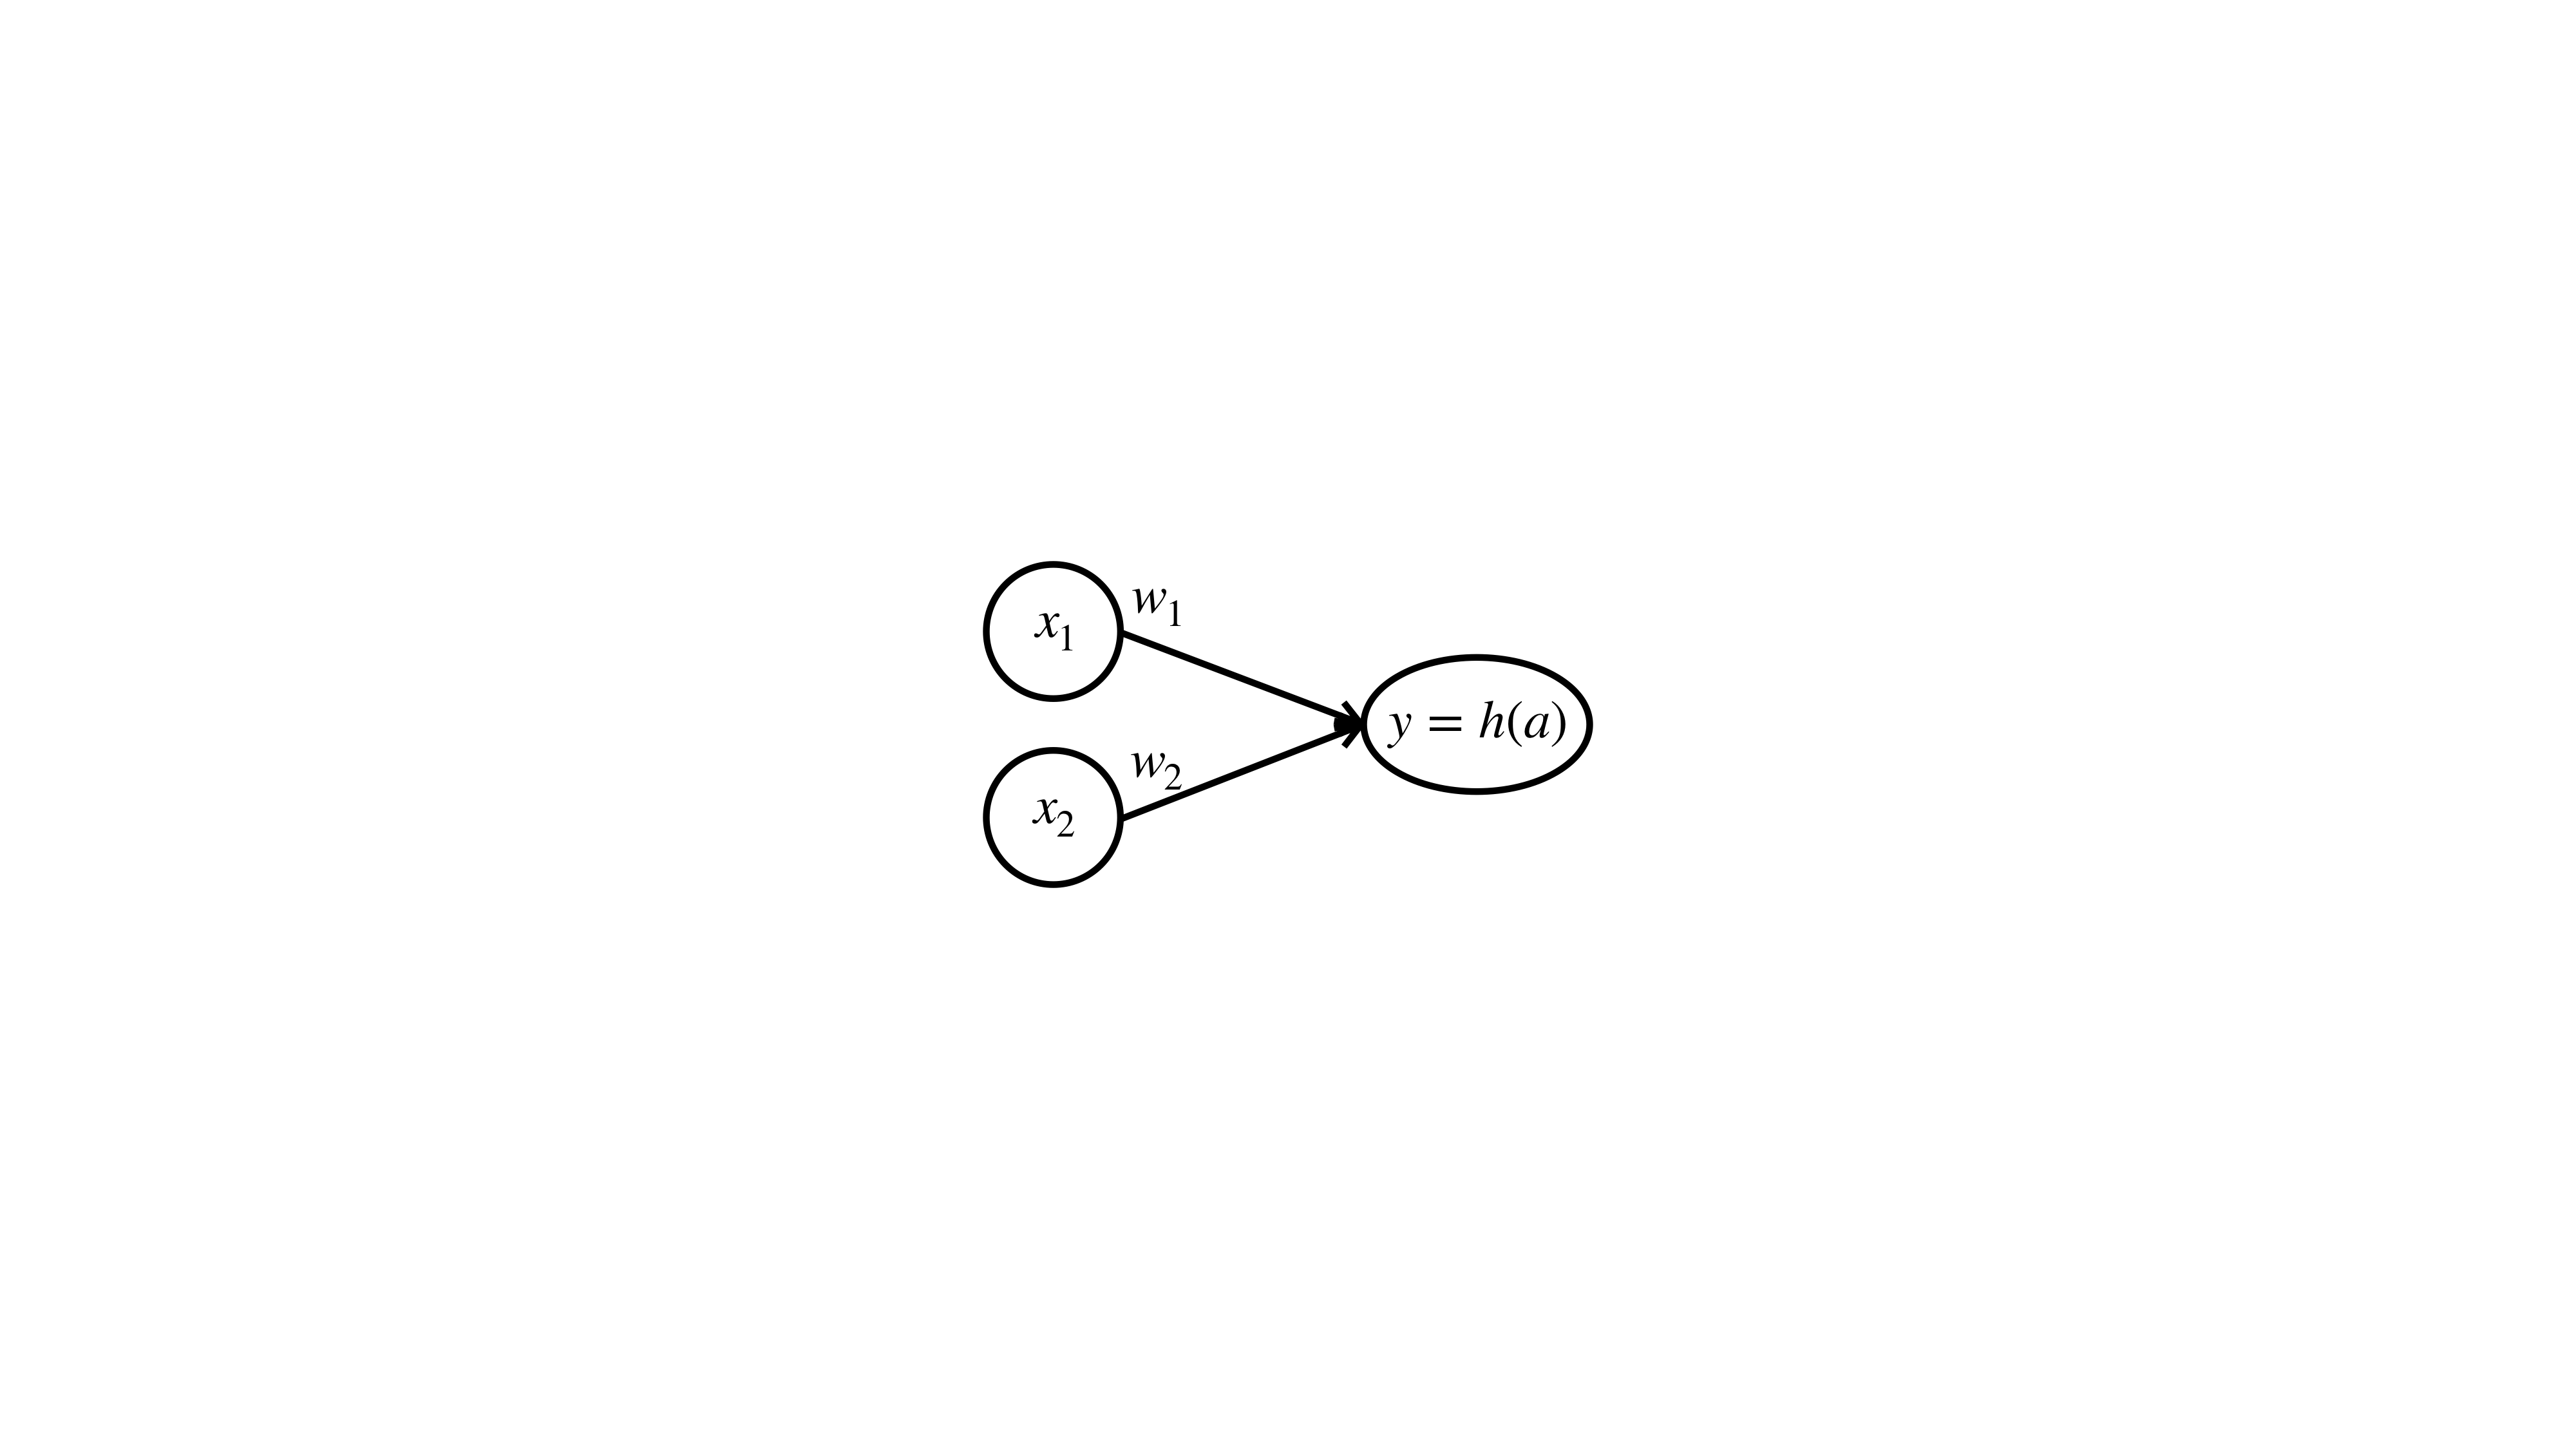
\includegraphics[trim = 250 350 250 350, width=0.9\textwidth, clip]{Figure/2DeepLearning/2SimplePerceptron.png}
 \caption[単純パーセプトロン]{単純パーセプトロン。入力を$x_1,x_2$, 出力を$y$と置いた。また, 各ノードの繋がりを矢印で表現し, 同時にそれぞれの線は学習可能な重みを表している。}
 \label{2SimplePerceptron}
\end{figure}

単純パーセプトロンの情報伝達は, 簡単な計算で定義される。
出力$y$は, $x_1,x_2$とそれぞれの重み$w_1,w_2$を用いて, 
\begin{equation}
 \begin{split}
  y &= h(a)\\
  a &= w_1x_1 + w_2x_2
 \end{split}
\end{equation}
と計算される。
ここで, 出力$y$は関数$h$によって変換されている。
このような関数を活性化関数 (Activation function) という。
特に単純パーセプトロンでは, 活性化関数$h$としてヘヴィサイドの階段関数(図\ref{3HeavisideStepFunction})を用いる。

\begin{figure}[htbp]
 \centering
 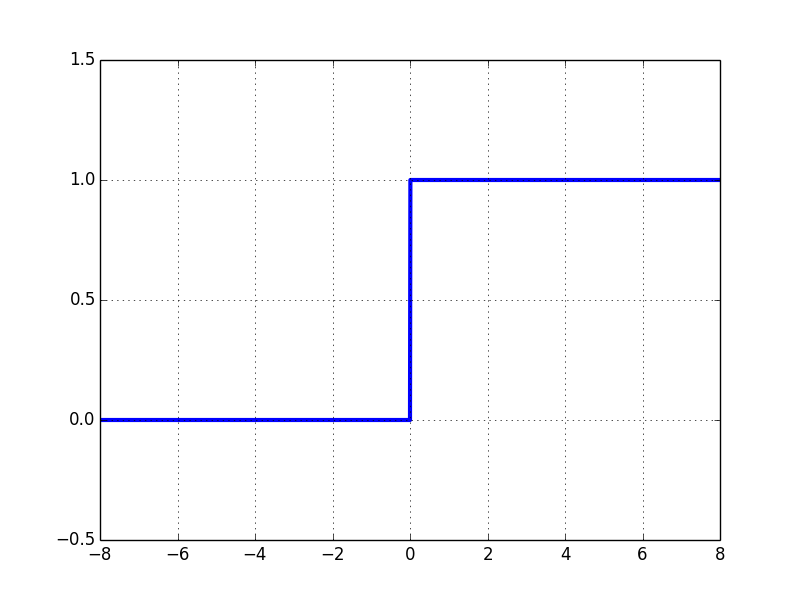
\includegraphics[width=0.5\textwidth]{Figure/2DeepLearning/3HeavisideStepFunction.png}
 \caption{ヘヴィサイドの階段関数}
 \label{3HeavisideStepFunction}
\end{figure}

その閾値を$\theta$とすると, 出力は更に, 
\begin{equation}
 y = h(a) = \left\{ \begin{array}{ll}
    0 & (a = w_1x_1 + w_2x_2 \leqq \theta) \\
    1 & (a = w_1x_1 + w_2x_2 > \theta)
 \end{array} \right.
\end{equation}
と書ける。
この時, 単純パーセプトロンはある一定値$\theta$までは``$0$", それ以上であれば``$1$"を返す二値信号のネットワークであると考えることが出来る。
パーセプトロンやニューラルネットワークにおいて, 学習可能なパラメータは重み$w_1,w_2$であり, これら重みを更新していく操作を学習 (トレーニング, Training) という。


%%%%%%%%%%%%%%%%%%%%%%%%%%%%%%%%%%%%%%%%%%%%%%%%%%%%%%%%%%%%%%%%%%%%%%%%
\subsection{多層パーセプトロン} \label{DL:Percep:MultiLayerPerceptron}

単純パーセプトロンは線形な問題を解く事しか出来なかったが, 層を重ねることで非線形に対応できるという点で非常に高い発展性を持っていた\cite{ApproximationSuperpositionsSigmoidalFunction}。
そのように単純パーセプトロンを重ねたネットワークの事を多層パーセプトロン (Multi Layer Perceptron, MLP) という。
多層パーセプトロンは図\ref{4MultiLayerPerceptron}のように表現出来る。

\begin{figure}[htbp]
 \centering
 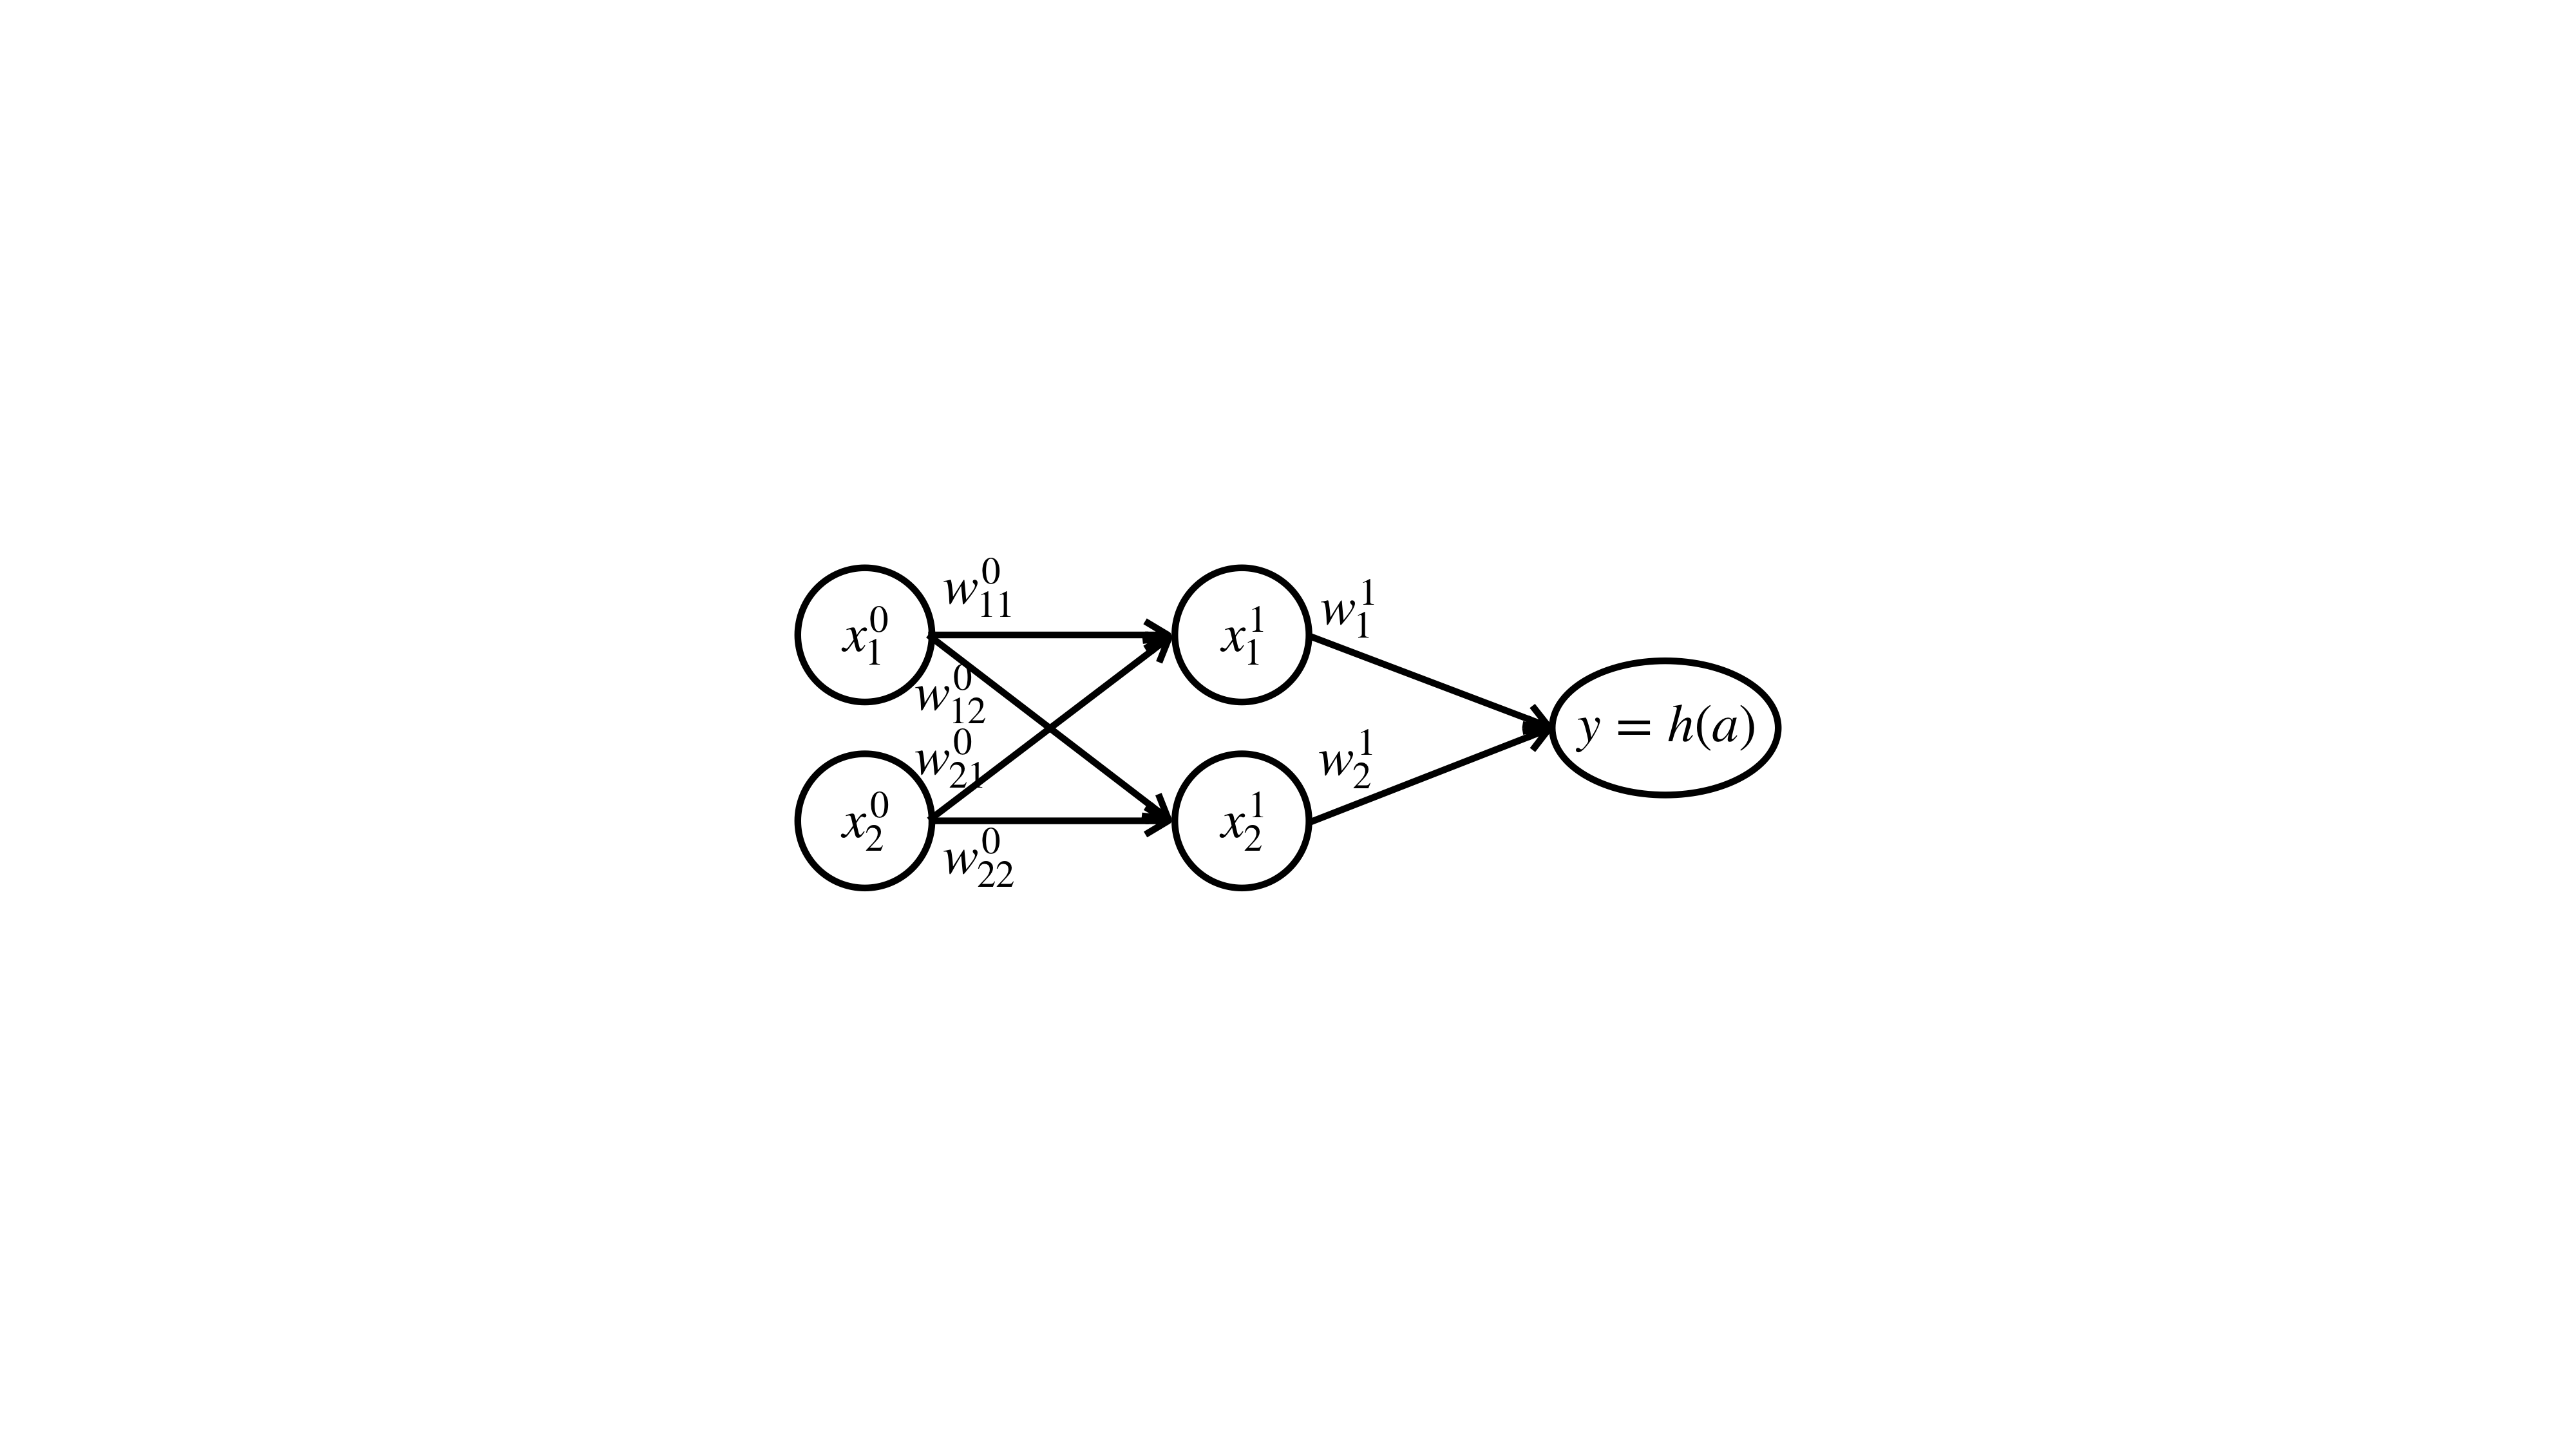
\includegraphics[trim = 250 350 250 350, width=0.9\textwidth, clip]{Figure/2DeepLearning/4MultiLayerPerceptron.png}
 \caption[多層パーセプトロン]{多層パーセプトロン。図\ref{2SimplePerceptron}と同様にノードを繋ぐそれぞれの線は学習可能な重みを表現している。前方のノードは後方のノードの全てと接続されている点にも注意が必要である。}
 \label{4MultiLayerPerceptron}
\end{figure}

多層パーセプトロンは単純パーセプトロンとは異なり, 入力, 出力以外に, 中間層 (隠れ層) を持っている。
ここで, 中間層を$x^1_1,x^1_2$と置くと, 単純パーセプトロンと同様に入力$x^0_1,x^0_2$とそれぞれの重み$w^0_{11},w^0_{12},w^0_{21},w^0_{22}$を用いて
\begin{equation}
 \begin{split}
  x^1_1 = w^0_{11}x^0_1 + w^0_{21}x^0_2 \\
  x^1_2 = w^0_{12}x^0_1 + w^0_{22}x^0_2
 \end{split} 
\end{equation}
と計算でき, また出力$y$についても, $x^1_1,x^1_2$とそれぞれの重み$w^1_{1},w^1_{2}$を用いて, 
\begin{equation}
 \begin{split}
  y &= h(a)\\
  a &= w^1_{1}x^1_1 + w^1_{2}x^1_2
 \end{split}
\end{equation}
となる。

以後, 特に断らない場合はあるノード$x$, 重み$w$について, 層の深さ, 前後のノードを次のように表現する。
\begin{equation}
 \begin{split}
  &x^{({\rm 層の深さ})}_{({\rm ノード番号})}\\
  &w^{({\rm 層の深さ})}_{({\rm 前のノード番号})\ ({\rm 後ろのノード番号})}
 \end{split}
\end{equation}

多層パーセプトロンは, 学習の手法や層を重ねるに連れて重みが更新出来なくなる勾配消失問題など様々な課題を抱えていた。
次節ではこれらの問題を後述する誤差逆伝播法 (Backpropagation) や活性化関数によって解決したニューラルネットワークについて解説する。


%%%%%%%%%%%%%%%%%%%%%%%%%%%%%%%%%%%%%%%%%%%%%%%%%%%%%%%%%%%%%%%%%%%%%%%%%%%%%%%%%%%%%%%%%%%%%%%%%%%%%
\section{ニューラルネットワーク} \label{DL:NeuralNetwork}

本節ではニューラルネットワークについて解説を行う。
ただし, ここでは計算手法や言葉の定義についてのみ述べる。
実装方法については現在様々なフレームワーク\cite{TensorflowWeb, KerasWeb, PyTorchWeb, CaffeWeb}があり, それぞれで実装の仕方が異なっている。
本研究ではtensorflow-kerasを用いた。\footnote{具体的なコードに関しては付録\ref{sec:Code}を参照。}

ニューラルネットワークに関する技術は「ニューラルネットワークの構造」についてと「ニューラルネットワークの学習」についてに大きく分けられると考えている。
前者は主に入力から出力までのネットワークの構築を, 後者は構築されたネットワークの重み更新についての技術である。


%%%%%%%%%%%%%%%%%%%%%%%%%%%%%%%%%%%%%%%%%%%%%%%%%%%%%%%%%%%%%%%%%%%%%%%%
\subsection{ニューラルネットワークの構造} \label{DL:NN:StructureofNN}

ニューラルネットワークは様々な技術によって支えられているが, その基本構造は前節の多層パーセプトロンと全く同じである。
ニューラルネットワークと多層パーセプトロンとの大きな構造の違いは活性化関数である。
ニューラルネットワークでは様々な活性化関数が提案されており\footnote{多層パーセプトロンはニューラルネットワークの内, 活性化関数に階段関数を使った特別なネットワークであると再定義できる。}, これが勾配消失問題を解消する鍵となっている。
活性化関数は重み更新のために微分可能な関数である必要があるが, どのような関数を選ぶかはユーザーに委ねられている。
勾配消失や重み更新についての詳しい解説は\ref{DL:NN:TrainingofNN}節で行う。
以下に活性化関数の例を示す(図\ref{5ActivationFunction})。
\begin{itemize}
  \item 階段関数
\begin{equation}
 h(a) = \left\{ \begin{array}{ll}
    0 & (a \leqq \theta) \\
    1 & (a > \theta)
 \end{array} \right.
\end{equation}
  \item シグモイド関数
\begin{equation}
 h(a) = \frac{1}{1+\exp{(-a)}}
\end{equation}
  \item tanh関数
\begin{equation}
 h(a) = \tanh{(a)}
\end{equation}
  \item ReLU (Rectified Linear Unit, ランプ) 関数\cite{ReLUpaper}
\begin{equation}
 h(a) = \left\{ \begin{array}{ll}
    0 & (a \leqq \theta) \\
    a & (a > \theta)
 \end{array} \right.
\end{equation}
\end{itemize}

\begin{figure}[htbp]
 \centering
 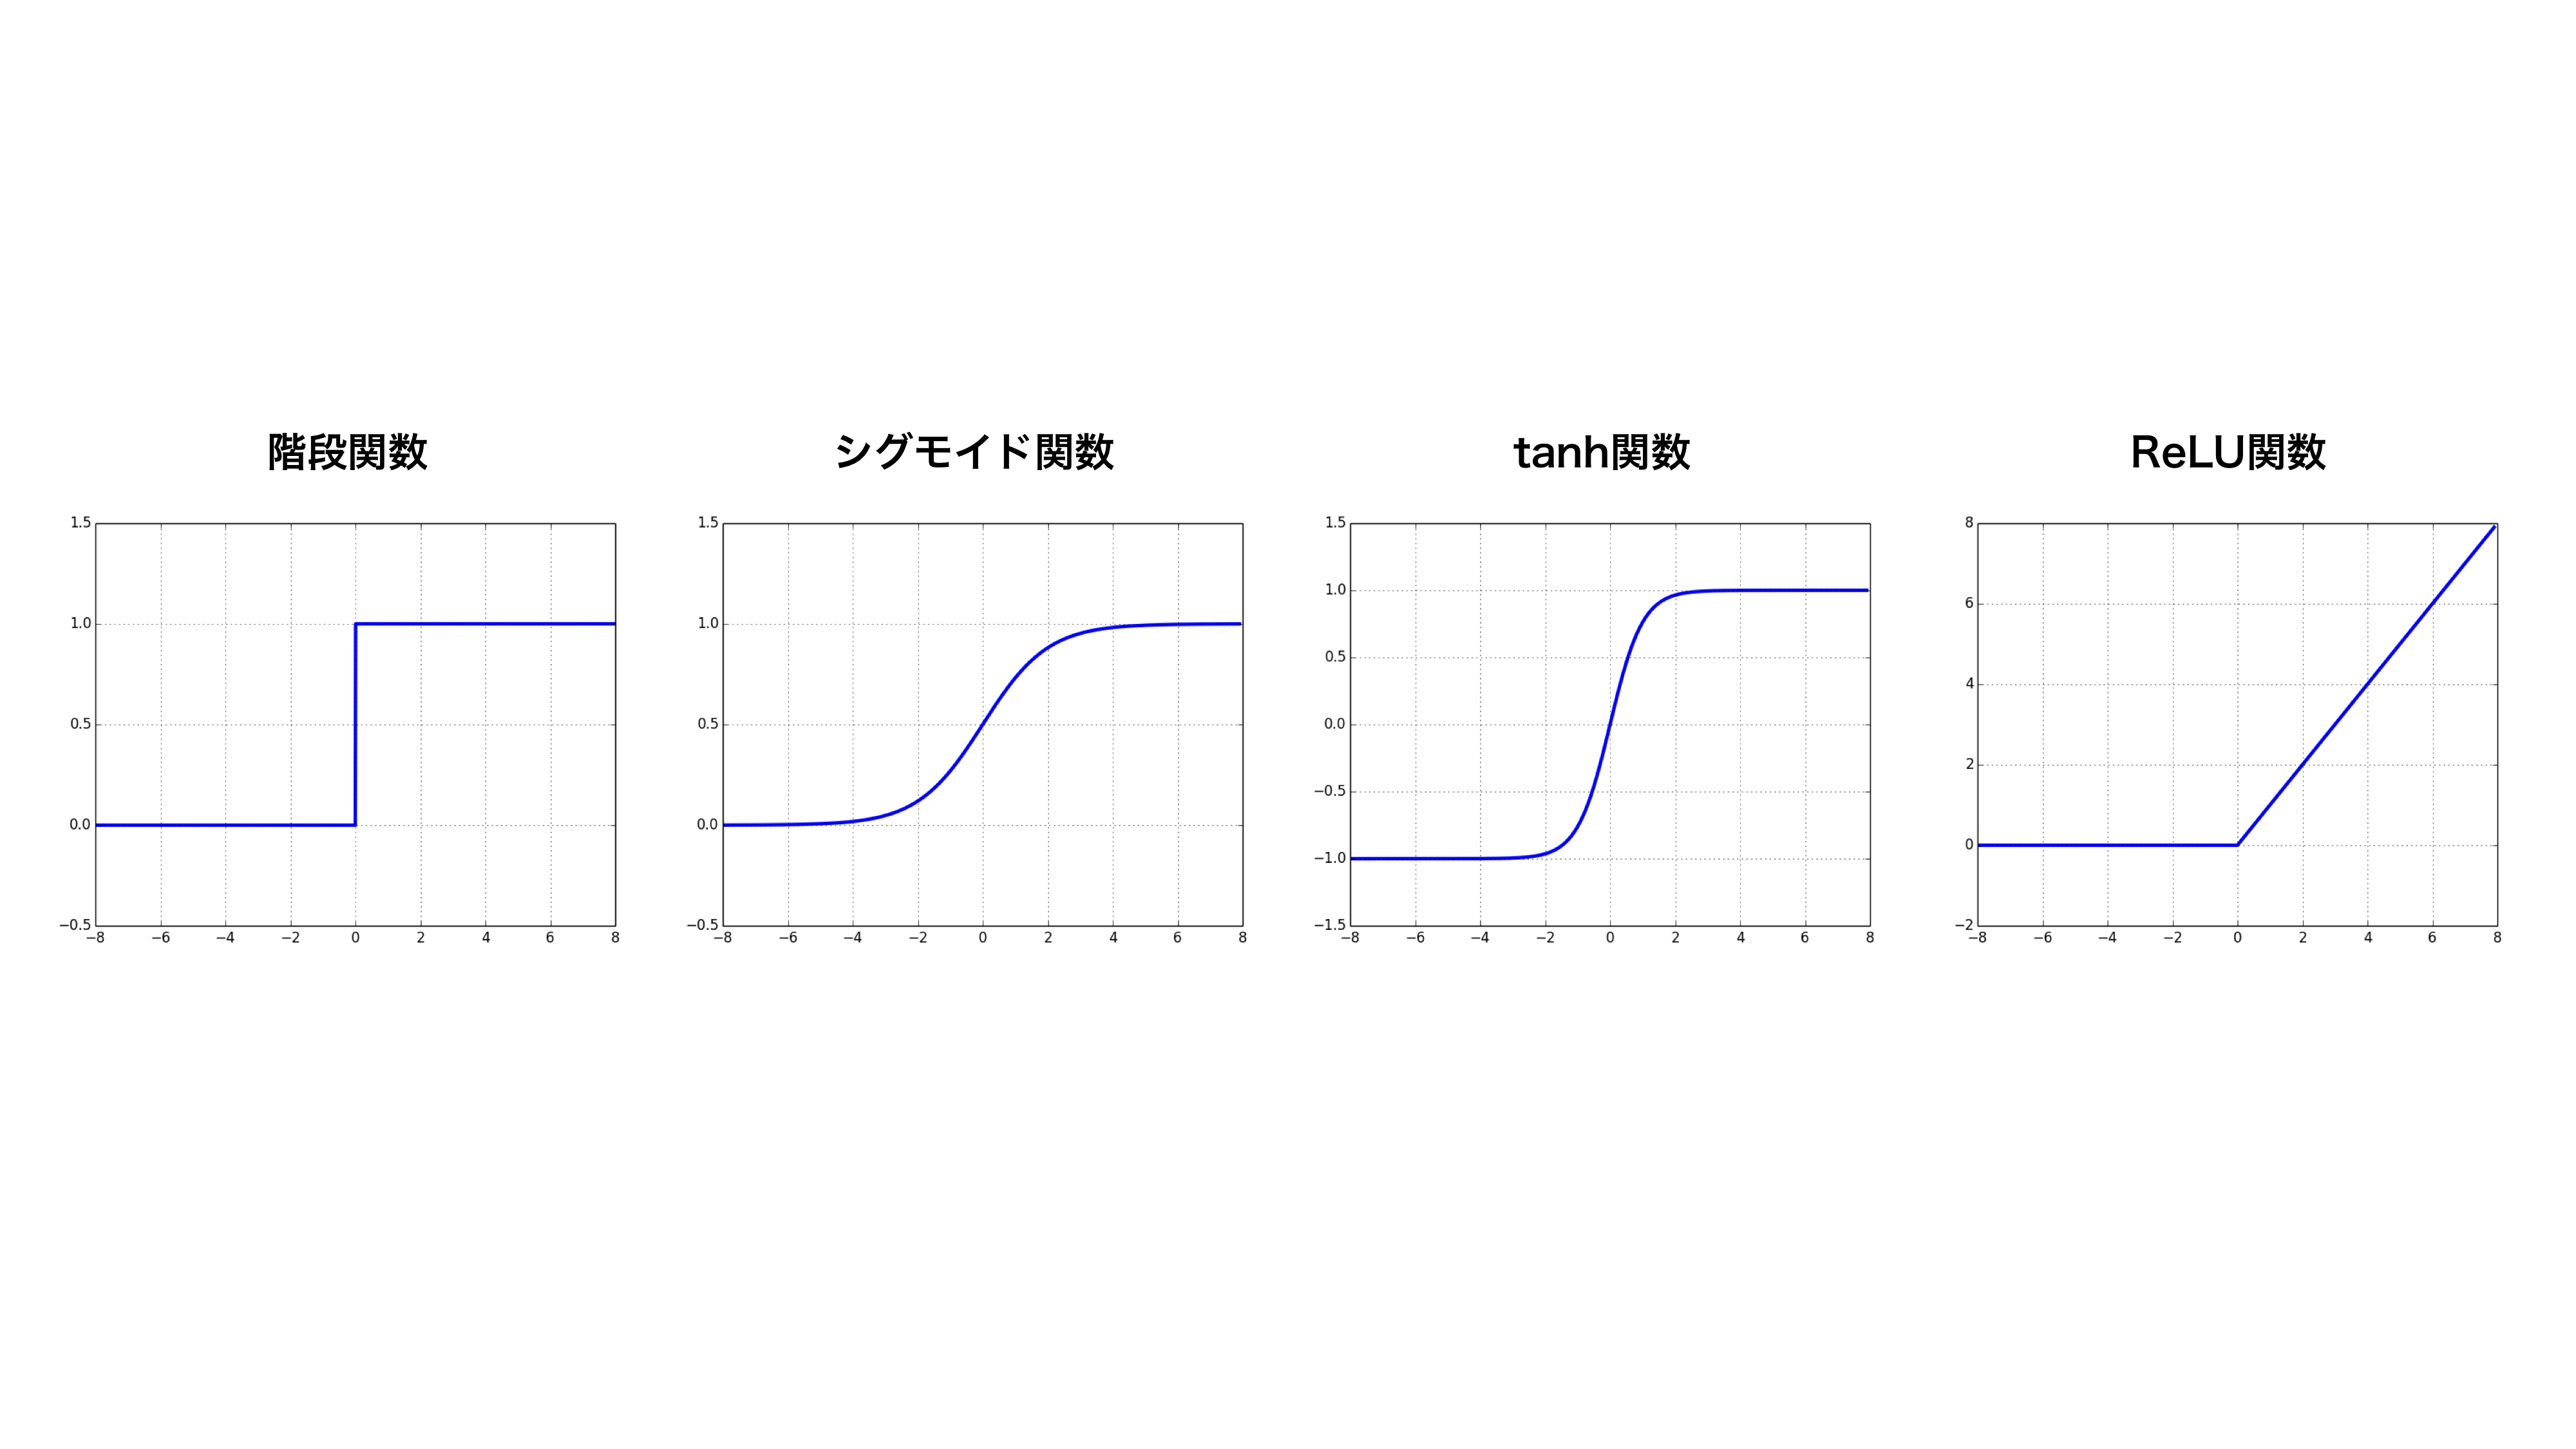
\includegraphics[trim = 0 250 0 250, width=1.0\textwidth, clip]{Figure/2DeepLearning/5ActivationFunction.png}
 \caption{活性化関数}
 \label{5ActivationFunction}
\end{figure}

一般に, ニューラルネットワークは多層パーセプトロンと同様の構造であるので, 図\ref{6NeuralNetwork}のように表現出来る。

\begin{figure}[htbp]
 \centering
 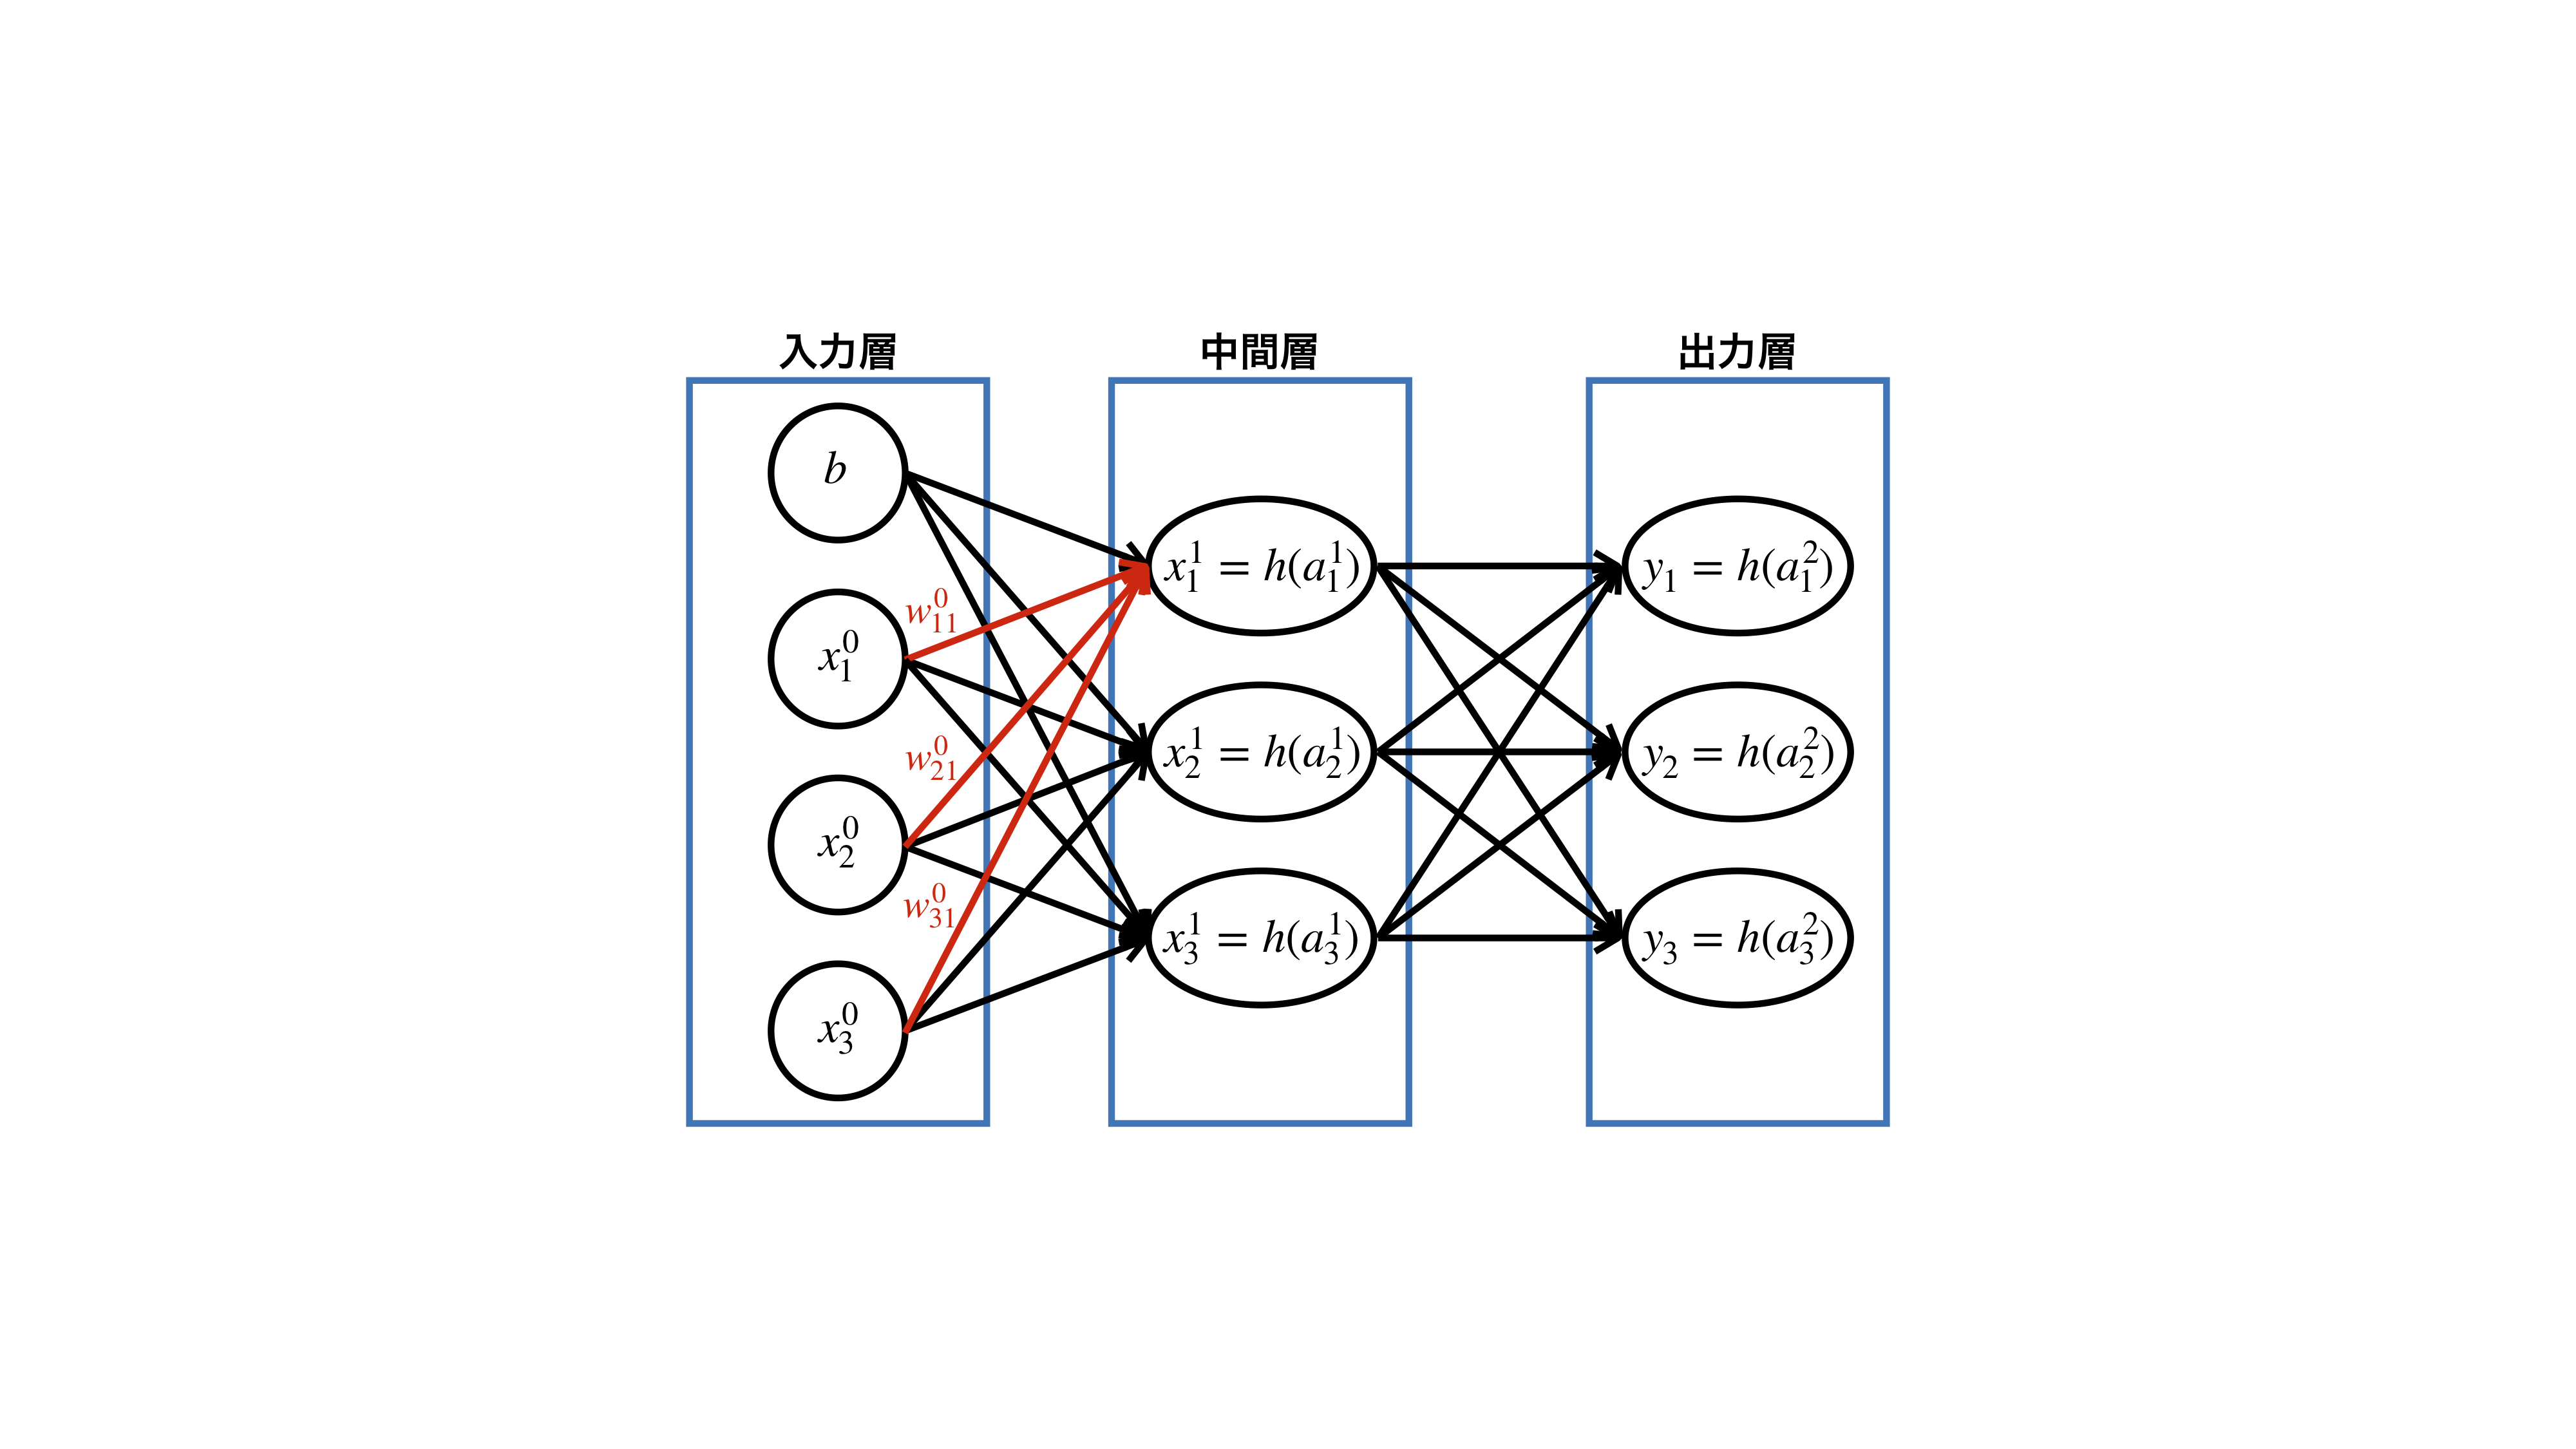
\includegraphics[trim = 250 200 250 200, width=0.9\textwidth, clip]{Figure/2DeepLearning/6NeuralNetwork.png}
 \caption[ニューラルネットワーク]{ニューラルネットワーク。基本構造は多層パーセプトロンと同様であるとわかる。赤線は中間層$x^1_1$へ入力される重みである。}
 \label{6NeuralNetwork}
\end{figure}

ここで, 中間層$x^1_1$は入力$x^0_1,x^0_2,x^0_3$とそれぞれの重み$w^0_{11},w^0_{21},w^0_{31}$を用いて, 
\begin{equation}
 \begin{split}
  x^1_1 &= h(a^1_1)\\
  a^1_1 &= w^0_{11}x^0_1 + w^0_{21}x^0_2 + w^0_{31}x^0_3 + b^0_1
 \end{split}
\end{equation}
と計算できる。
また, バイアスとして$b$を導入している。
これはパーセプトロンの閾値$\theta$に対応している。
中間層$x^1_2,x^1_3$についても同様に, 
\begin{equation}
 \begin{split}
  x^1_2 &= h(a^1_2)\\
  a^1_2 &= w^0_{12}x^0_1 + w^0_{22}x^0_2 + w^0_{32}x^0_3 + b^0_2\\
  x^1_3 &= h(a^1_3)\\
  a^1_3 &= w^0_{13}x^0_1 + w^0_{23}x^0_2 + w^0_{33}x^0_3 + b^0_3
 \end{split}
\end{equation}
と書ける。

また, これら$x^1_1,x^1_2,x^1_3$の計算は行列とベクトルを用いて, より簡潔に表現できる。
\begin{equation}
 \begin{split}
  {\mbox{\boldmath{$x$}}}^1&=
  \left(
    \begin{array}{ccc}
      x^1_1 \\
      x^1_2 \\
      x^1_3 
    \end{array}
  \right)=
  h({\mbox{\boldmath{$a$}}}^1)\\
  {\mbox{\boldmath{$a$}}}^1&=
  \left(
    \begin{array}{ccc}
      a^1_1 \\
      a^1_2 \\
      a^1_3 
    \end{array}
  \right)
  =
  W^0{\mbox{\boldmath{$x$}}}^0 + {\mbox{\boldmath{$b$}}}^0
  =
  \left(
    \begin{array}{ccc}
      w^0_{11} & w^0_{21} & w^0_{31} \\
      w^0_{12} & w^0_{22} & w^0_{32} \\
      w^0_{13} & w^0_{23} & w^0_{33}
    \end{array}
  \right)
  \left(
    \begin{array}{ccc}
      x^0_1 \\
      x^0_2 \\
      x^0_3
    \end{array}
  \right)
  +
  \left(
    \begin{array}{ccc}
      b^0_1 \\
      b^0_2 \\
      b^0_3
    \end{array}
  \right)
 \end{split}
\end{equation}
行列$W^0$とベクトル${\mbox{\boldmath{$b$}}}^0$は学習可能な重みであり, 得られた新たな状態ベクトル${\mbox{\boldmath{$a$}}}^1$は微分可能な任意の活性化関数$h$によって, 中間層${\mbox{\boldmath{$x$}}}^1$へと変換される。
以下, これを繰り返すことによって, ネットワークは構築されている。

出力層における活性化関数は一般に回帰問題では恒等関数を, 分類問題ではソフトマックス関数と呼ばれる関数を使用する。
回帰問題において, 最終的な出力は数値 (連続値) であるため, 恒等関数によって, 変換を行わずそのまま出力することが一般である。

\begin{equation}
 y_k = h(a^2_k) = a^2_k
\end{equation}

一方で, 分類問題では, 最終的な出力は分類されたクラスとなるため, 以下のようなソフトマックス関数を使用する。

\begin{equation}
 y_k = h(a^2_k) = \frac{\exp{(a^2_k)}}{\sum^N_{i=1}\exp{(a^2_i)}}
\end{equation}

このソフトマックス関数は, 分母が総和, 分子がその一要素の形をしており, $y_k$をkについて足し合わせると$1$になることがわかる。
このことから, 出力$y_k$はk番目のクラスについての確率として解釈でき, 分類問題において, どのクラスにどの程度該当するかを表現することに相当している。

前述したように, これは最も基本的なニューラルネットワークであり, このような全結合 (Fully connected, Dense) な層を重ねたネットワークを順伝播型 (フィードフォワード) ニューラルネットワーク (Feedforward Neural Network) という。


%%%%%%%%%%%%%%%%%%%%%%%%%%%%%%%%%%%%%%%%%%%%%%%%%%%%%%%%%%%%%%%%%%%%%%%%
\subsection{ニューラルネットワークの学習} \label{DL:NN:TrainingofNN}


教師あり学習であるニューラルネットワークにおける学習は, 損失関数 (コスト関数, Loss function) を最小化するように, 重みを更新していく事で行われる。
損失関数とは, 訓練データの正解ラベルとネットワークの出力がどの程度離れているかを計算するための関数である。
この損失関数は取り組む問題や訓練データの性質によって適切に選択する必要がある。
ここでは, よく使用される損失関数として以下の二つを挙げる。
\begin{itemize}
  \item 交差エントロピー誤差 (Categorical Cross Entropy)
\begin{equation}
 L = - \sum^N_k t_k \log{(y_k)}
\end{equation}
  \item 平均二乗誤差 (Mean Squared Error)
\begin{equation}
 L = \frac{1}{N} \sum^N_k(t_k - y_k)^2
\end{equation}
\end{itemize}
$t_k, y_k$はそれぞれk番目の正解ラベルとクラスの出力 (確率や値) を示している。
分類問題については交差エントロピー誤差が, 回帰問題については平均二乗誤差が主に使用される。

分類問題において, 正解ラベル$t$は, あるクラスに関して0か1かのベクトル (one-hot vector) で表現されることが一般的である。
例えば, 赤, 青, 緑について分類を行う場合 (3クラス分類という) , 赤を$(1, 0, 0)$, 青を$(0, 1, 0)$, 緑を$(0, 0, 1)$と定義する。
また, ネットワークの出力$y$はどのクラスに属するかの確率となっている。
例えば, 赤, 青, 緑がそれぞれ$80\ \%$, $10\ \%$, $10\ \%$の場合は出力$y$は$(0.8,\ 0.1,\ 0.1)$と書ける。
したがって, 正解ラベルを赤とすると損失関数$L$は
\begin{equation}
 \begin{split}
  L &= - \sum^3_k t_k \log{(y_k)} \\
    &= - t_1 \log{y_1} - t_2 \log{y_2} - t_3 \log{y_3} \\
    &= - 1 \cdot \log{0.8}\\
    &= 0.22314...
 \end{split}
\end{equation}
と計算される。

回帰問題において, 出力$y$, 正解ラベル$t$は共に連続値であるため, 平均二乗誤差のような二つの差を用いる損失関数が一般的である。

前述したように, ネットワークの学習はこの損失関数を最小化するように進む。
今, 損失関数は変数$y_k$の関数で表現出来ており, このような関数の最小値を求めるためには, 単に変数$y_k$を用いて偏微分を行い勾配を求めれば良い。
計算機において, このような勾配を求め, 徐々に関数を最小化していく手法を勾配降下法 (Gradient Descent Method) という。
勾配降下法において, 次のステップの変数$y_k'$は次のように計算される。
\begin{equation}
 \begin{split}
  y_k' = y_k - \eta \frac{\partial L}{\partial y_k}
 \end{split}
\end{equation}
ここで, ステップ幅を決定する定数$\eta$をニューラルネットワークにおいて学習率 (learning rate) という。
学習率は0.001などの定数を問題やネットワークによって適切に選ぶ必要がある。
このようなネットワークについて更新されない初期設定のパラメータをハイパーパラメータという。
ハイパーパラメータについては後の\ref{DL:HyperParameter}節で述べる。

ニューラルネットワークにおいて, 各重みを更新するための勾配は連鎖律 (chain rule) を用いて計算される。
これは更新する重みと最小化される損失関数の間に出力層と活性化関数が存在しているためである。\footnote{損失関数はクラスの出力の関数であり, クラスの出力は活性化関数によって計算され, 活性化関数は出力層の関数である。}
具体的には, ある重み行列$W$に対して, 勾配降下法, 連鎖律を考慮すると, 次のステップの重み行列$W'$は
\begin{equation}
 \begin{split}
  W' &= W - \eta \frac{\partial L}{\partial W}\\
    &=
  \left(
    \begin{array}{ccc}
      w_{11} & w_{21} & w_{31} \\
      w_{12} & w_{22} & w_{32} \\
      w_{13} & w_{23} & w_{33}
    \end{array}
  \right)
  - \eta
  \left(
    \begin{array}{ccc}
      \frac{\partial L}{\partial w_{11}} & \frac{\partial L}{\partial w_{21}} & \frac{\partial L}{\partial w_{31}} \\
      \frac{\partial L}{\partial w_{12}} & \frac{\partial L}{\partial w_{22}} & \frac{\partial L}{\partial w_{32}} \\
      \frac{\partial L}{\partial w_{13}} & \frac{\partial L}{\partial w_{23}} & \frac{\partial L}{\partial w_{33}}
    \end{array}
  \right)\\
    &= W - \eta \frac{\partial L}{\partial y}\frac{\partial y}{\partial a}\frac{\partial a}{\partial W}
 \end{split}
\end{equation}
と計算される。

このような最適化問題に関して, いくつかのアルゴリズムが提案されている。
現在は確率的勾配降下法 (Stochastic Gradient Descent, SGD\cite{SGD}) やそれを基礎としたRMSProp\cite{RMSProp}, Adam\cite{Adam}などの手法がよく使用されている。

学習方法における, ニューラルネットワークと多層パーセプトロンの大きな違いは, 重みの更新を出力層から逆伝播させる誤差逆伝播法 (Backpropergation\cite{Backpropagation}) という手法の有無である。
再度, 図\ref{6NeuralNetwork}を考える。
全ての出力, 中間層を行列計算を用いて記述すると, 
\begin{equation}
 \begin{split}
  {\mbox{\boldmath{$a$}}}^1&=
  \left(
    \begin{array}{ccc}
      a^1_1 \\
      a^1_2 \\
      a^1_3 
    \end{array}
  \right)
  =
  W^0{\mbox{\boldmath{$x$}}}^0 + {\mbox{\boldmath{$b$}}}^0
  =
  \left(
    \begin{array}{ccc}
      w^0_{11} & w^0_{21} & w^0_{31} \\
      w^0_{12} & w^0_{22} & w^0_{32} \\
      w^0_{13} & w^0_{23} & w^0_{33}
    \end{array}
  \right)
  \left(
    \begin{array}{ccc}
      x^0_1 \\
      x^0_2 \\
      x^0_3
    \end{array}
  \right)
  +
  \left(
    \begin{array}{ccc}
      b^0_1 \\
      b^0_2 \\
      b^0_3
    \end{array}
  \right)\\
  {\mbox{\boldmath{$x$}}}^1&=h({\mbox{\boldmath{$a$}}}^1)\\
  {\mbox{\boldmath{$a$}}}^2&=
  \left(
    \begin{array}{ccc}
      a^2_1 \\
      a^2_2 \\
      a^2_3 
    \end{array}
  \right)
  =
  W^1{\mbox{\boldmath{$x$}}}^1
  =
  \left(
    \begin{array}{ccc}
      w^1_{11} & w^1_{21} & w^1_{31} \\
      w^1_{12} & w^1_{22} & w^1_{32} \\
      w^1_{13} & w^1_{23} & w^1_{33}
    \end{array}
  \right)
  \left(
    \begin{array}{ccc}
      x^1_1 \\
      x^1_2 \\
      x^1_3
    \end{array}
  \right)\\
 y_k &= \sigma(a^2_k) = \frac{\exp{(a^2_k)}}{\sum^n_{i=1}\exp{(a^2_i)}}
 \end{split}
\end{equation}
と書ける。
ここで, 出力部分のソフトマックス関数を$\sigma$と書いた。

ある重み$w^1_{11}$について考える。
損失関数$L$の重み$w^1_{11}$による偏微分は, 連鎖律を考慮して, 
\begin{equation}
 \begin{split}
  y_1 &= \sigma(a^2_1)\\
  a^2_1 &= w^1_{11} x^1_1 + w^1_{21} x^1_2 + w^1_{31} x^1_3 = \sum^N_{i=1} w^1_{i1} x^1_i
 \end{split}
\end{equation}
より, 
\begin{equation}
 \begin{split}
  \frac{\partial L}{\partial w^1_{11}} 
  &= \frac{\partial L}{\partial y_1}\frac{\partial y_1}{\partial a^2_1}\frac{\partial a^2_1}{\partial w^1_{11}}\\
  &= \frac{\partial L}{\partial y_1}\frac{\partial \sigma(a^2_1)}{\partial a^2_1}x^1_{11}\\
 \end{split}
\end{equation}
と計算できる。

ここで, 勾配の計算に活性化関数の偏微分が常に積の形で含まれていることがわかる。
この活性化関数の偏微分が$0$になり, そこから抜け出せなくなると, その勾配は常に$0$になり消失してしまう, これが勾配消失である。
勾配消失に陥った場合は, 重みが適切に更新されず, 学習が不十分になってしまう。
このような問題は活性化関数を変更することによって改善され, 現在はReLU関数がよく用いられている。

また, 更に浅い層の重み$w^0_{11}$について考えると, 
\begin{equation}
 \begin{split}
  x^2_1 &= h(a^1_1)\\
  a^1_1 &= w^0_{11} x^0_1 + w^0_{21} x^0_2 + w^0_{31} x^0_3 = \sum^N_{i=1} w^1_{i1} x^0_i
 \end{split}
\end{equation}
より, 
\begin{equation}
 \begin{split}
  \frac{\partial L}{\partial w^0_{11}} 
  &= \sum^N_{k} \frac{\partial L}{\partial y_k}\frac{\partial y_k}{\partial a^2_k}\frac{\partial a^2_k}{\partial x^2_1}\frac{\partial x^2_1}{\partial a^1_1}\frac{\partial a^1_1}{\partial w^0_{11}}\\
  &= \sum^N_{k} \frac{\partial L}{\partial y_k}\frac{\partial y_k}{\partial a^2_k}\frac{\partial a^2_k}{\partial x^2_1}\frac{\partial h(a^1_1)}{\partial a^1_1}x^0_{11}\\
  &= \sum^N_{k} \left(\frac{\partial L}{\partial y_k}\frac{\partial y_k}{\partial a^2_k}w^1_{1k}\right)\frac{\partial h(a^1_1)}{\partial a^1_1}x^0_{11}
 \end{split}
\end{equation}
と計算できる。
この計算は更に層を重ねた場合でも同様の手順で行うことができる。

重みの更新は基本的に全ての訓練データを使用するのではなく, 訓練データをいくつかの塊に分け, その塊について損失関数を計算することで行われる。
このような手法をミニバッチ学習と呼ばれる。
(訓練データ全てを用いたものをバッチ学習という。)
ミニバッチ学習に使用されるデータの数をミニバッチサイズ (あるいは単にバッチサイズ) という。
これも後述するハイパーパラメータの一つである。
ミニバッチ学習はバッチ学習と比較して二つの利点が存在する。

一つは膨大なデータを直接処理しなくても良いという点である。
一般に深層学習で使用されるデータは非常に膨大であり, GPUなどのメモリに乗らない場合があるが, ミニバッチ学習ではこれを回避することができる。

もう一つは学習が停滞しづらいという点である。
訓練データと比較してサイズの小さいミニバッチは上記の勾配が0になりづらく, 局所的な最小点での学習の停滞を回避することができる。

ただしミニバッチ学習のバッチサイズが小さくなった場合には, 損失関数が平均化されず学習が不安定になる (収束しなくなる) という問題が生じる場合がある。\footnote{バッチサイズが$1$ ($1$サンプルのみ) のミニバッチ学習をオンライン学習という。}


%%%%%%%%%%%%%%%%%%%%%%%%%%%%%%%%%%%%%%%%%%%%%%%%%%%%%%%%%%%%%%%%%%%%%%%%
\subsection{ディープニューラルネットワーク} \label{DL:NN:DeepNeuralNetwork}

ディープニューラルネットワーク (Deep Neural Network, DNN) という言葉の定義は非常に曖昧である。\footnote{少なくとも私ははっきりとした定義を存じない。}
\ref{DL:MachineandDeepLearning}節で述べたように, 現在は第三期AIブームであると言われている。
これは上述してきた技術的成熟に加え, 計算機の性能が向上したことにより, より層を重ねた (深い) ニューラルネットワークの学習が可能になった結果であると言える。
$2006$年のHintonらによるauto-encoder\cite{Autoencoder}や$2014$年にIanによって提案された敵対的生成ネットワーク (Generative Adversarial Network, GAN\cite{GenerativeAdversarialNetworks}) など, 様々な発展的な応用がなされ, 現在においても毎年のように新しいネットワークが提案されている。
本節で述べたニューラルネットワークはその基盤技術の一部である。
次節以降では, 系列データを扱うためのニューラルネットワークの応用について紹介する。


%%%%%%%%%%%%%%%%%%%%%%%%%%%%%%%%%%%%%%%%%%%%%%%%%%%%%%%%%%%%%%%%%%%%%%%%%%%%%%%%%%%%%%%%%%%%%%%%%%%%%
\section{リカレントニューラルネットワーク} \label{DL:RecurrentNeuralNetwork}

前節で紹介したようなフィードフォワードニューラルネットワークは系列データを扱う際, 重み行列が固定的な大きさでしか保持出来ないという点と直前の系列に依存した学習が出来ないという点に関して課題を抱えている。
これらの課題を解決するために提案されたのが, リカレントニューラルネットワークというネットワーク構造である。
本節では, このリカレントニューラルネットワークについて解説を行う。
リカレントニューラルネットワークは主に系列データ, 特に時系列データを取り扱うためのネットワークである。
このような時系列に関するニューラルネットワークは自然言語処理などの分野で発展し, 音声認識や機械翻訳といった技術に使用されている。
リカレントニューラルネットワークの構造は, フィードフォワードニューラルネットワークと比較すると複雑であるが, 要素計算は全結合であり, 基本的にはその組み合わせで理解できる。
\ref{DL:RNN:ReccurentNeuralNetwork}項では, そのようなリカレントニューラルネットワークの構造と学習について述べる。
その後, リカレントニューラルネットワークの抱える問題と, ゲート (Gate) と記憶セル (Cell) 呼ばれる技術によってその問題を克服した長・短期記憶 (Long Short-Term Memory, LSTM\cite{LSTMpaper}) というネットワークを\ref{DL:RNN:IssueofRNN}項と\ref{DL:RNN:LongShortTermMemory}項でそれぞれ紹介する。


%%%%%%%%%%%%%%%%%%%%%%%%%%%%%%%%%%%%%%%%%%%%%%%%%%%%%%%%%%%%%%%%%%%%%%%%
\subsection{リカレントニューラルネットワークの構造と学習} \label{DL:RNN:ReccurentNeuralNetwork}

リカレントニューラルネットワークの構造は, これまでのフィードフォワードニューラルネットワークとは大きく異なる。
そのネットワーク構造はいくつかの表現方法が存在しているが, 本論文では時間について展開した図で書くこととする。
図\ref{7RecurrentNeuralNetwork}の左側が時間について展開していない図, 右側が時間について展開した図である。
左側では, 時間についての構造をループで表現し, 任意の時間$t$についての入力$x_t$と出力$h_t$を持つネットワークとして表現している。
右側では, 時間についての構造を展開し, 出力や入力を系列情報とともに表現している。
これまでのフィードフォワードネットワークは情報の伝達を左右に描いていたが, このリカレントニューラルネットワークは上下に描き, 系列の流れを左右で表現されることが多い。
図\ref{7RecurrentNeuralNetwork}の右側では, 出力$h$が二つ存在し, 上に進むものを出力に, 右に進むものが次の系列への入力になっていることがわかる。
このように, 現在の出力を次の系列の入力として使うことで, 直前の系列情報への依存性を導入している。

\begin{figure}[htbp]
 \centering
 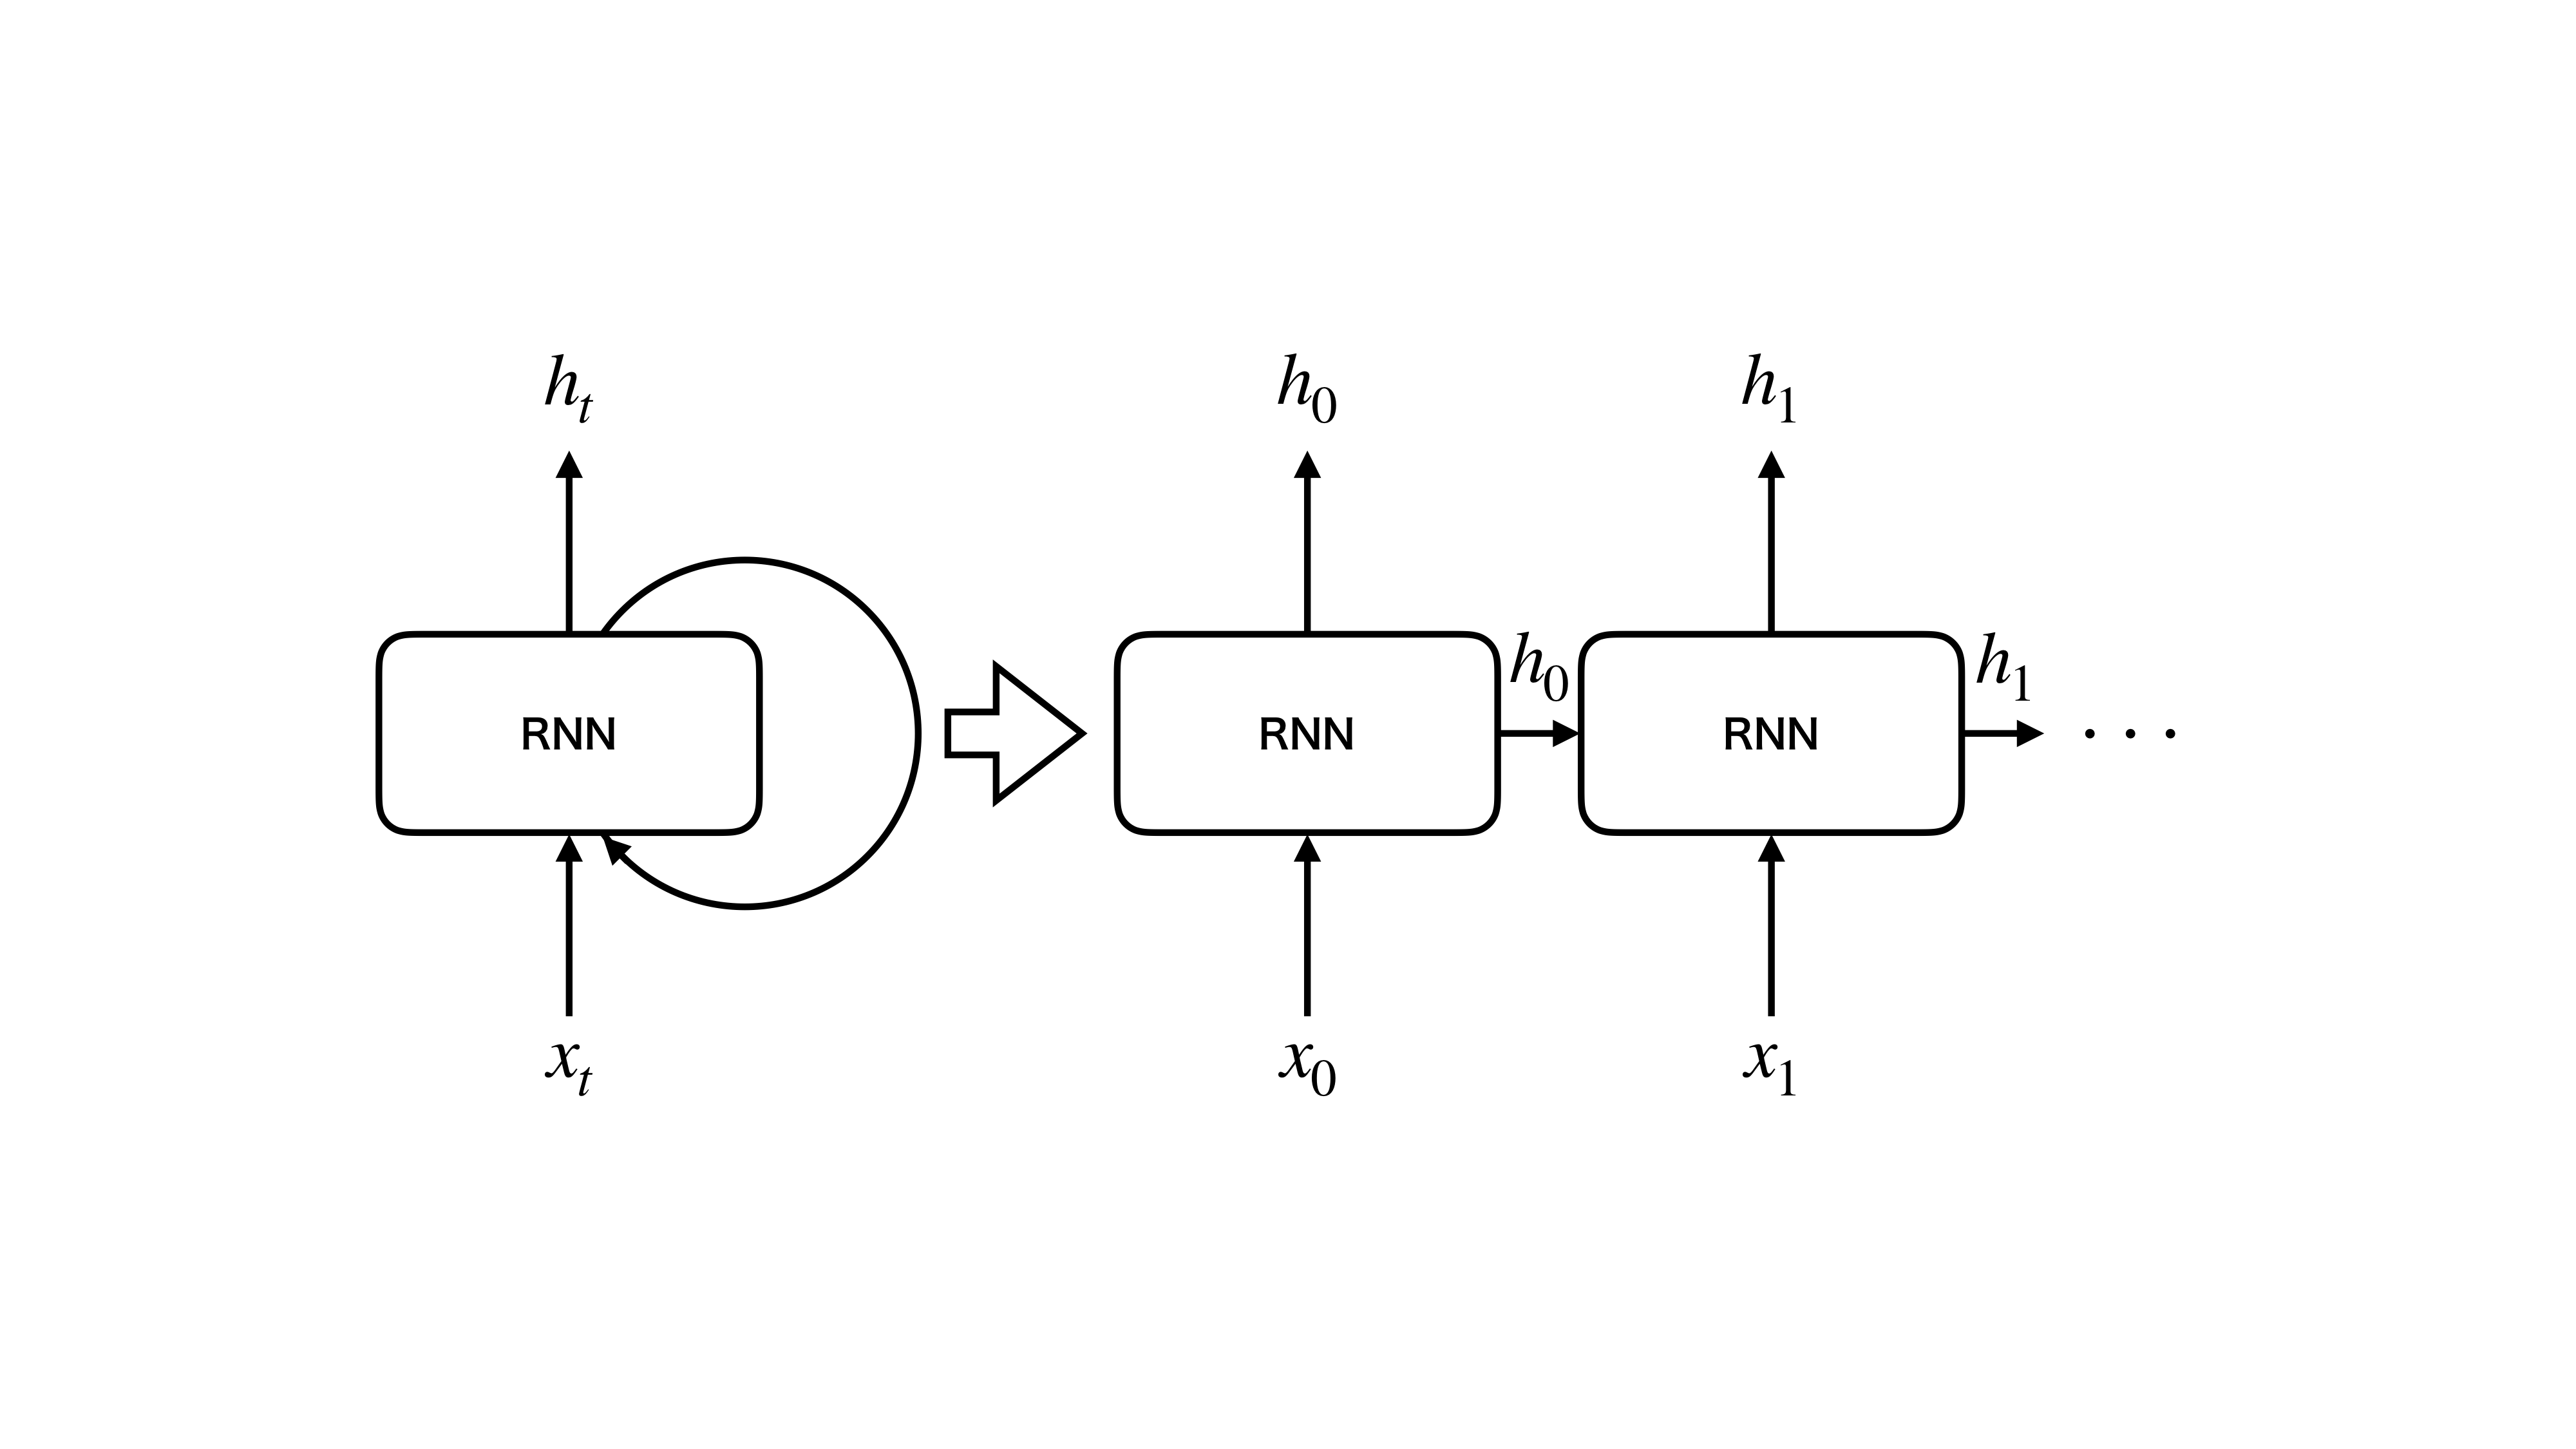
\includegraphics[trim = 0 200 0 200, width=0.9\textwidth, clip]{Figure/2DeepLearning/7RecurrentNeuralNetwork.png}
 \caption[リカレントニューラルネットワーク]{リカレントニューラルネットワーク。図左は時間について展開していない描画方法, 図右は時間について展開した描画方法である。下方から入力され, 上方に出力している。横方向は系列を表現しており, 入力$x_t$は全ての系列で同じ形状でなければならない。}
 \label{7RecurrentNeuralNetwork}
\end{figure}

これまでと同様に明示的にネットワークの重みを描画すると, 図\ref{8RNNWeight}のようになる。
図\ref{7RecurrentNeuralNetwork}のRNNに当たる部分が展開され, 重みを線で表現した図になっている。
図より, 一つ前に系列の出力${\mbox{\boldmath{$h$}}}_{t-1}$と現在の系列の入力${\mbox{\boldmath{$x$}}}_t$を用いて, 現在の系列の出力${\mbox{\boldmath{$h$}}}_t$が生成されていることがわかる。
${\mbox{\boldmath{$h$}}}$についての赤い線に関する重み行列を$W_h$, ${\mbox{\boldmath{$x$}}}$についての黒い線に関する重み行列を$W_x$と置くと, 出力${\mbox{\boldmath{$h$}}}_t$は次のように計算できる。

\begin{figure}[htbp]
 \centering
 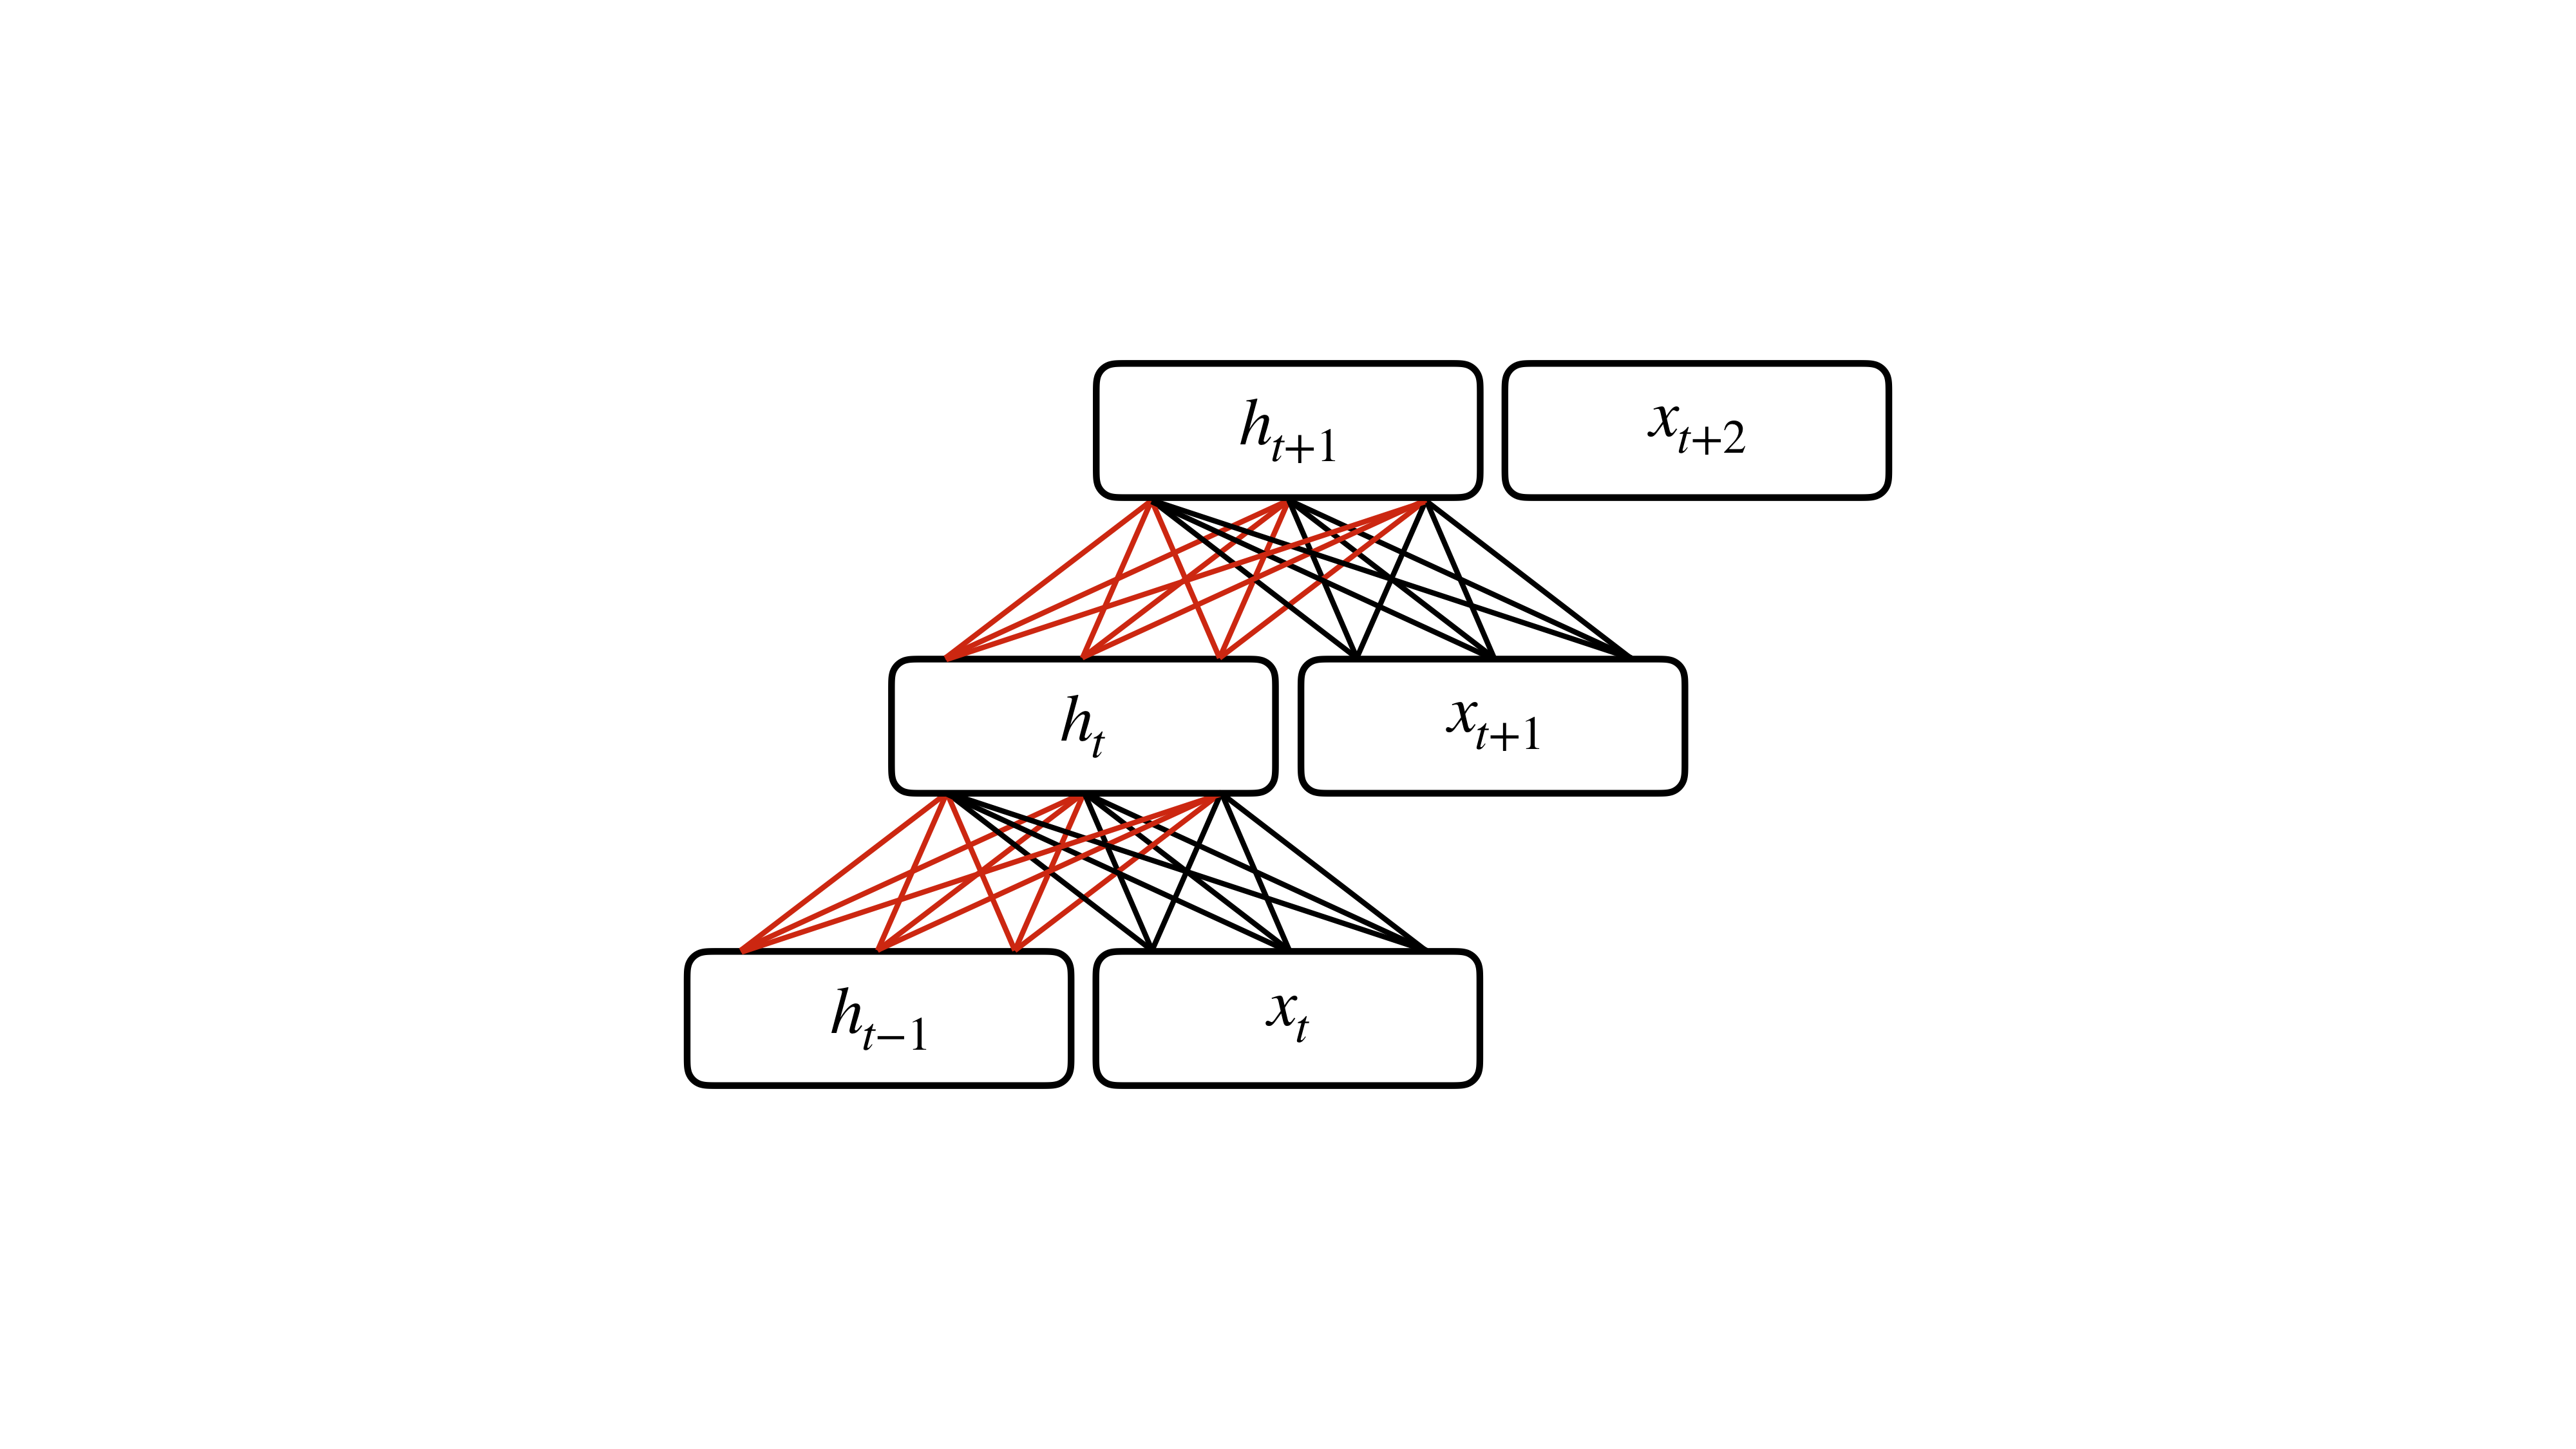
\includegraphics[trim = 0 200 0 200, width=0.9\textwidth, clip]{Figure/2DeepLearning/8RNNWeight.png}
 \caption[リカレントニューラルネットワークの重みの明示的な表現]{リカレントニューラルネットワークの重みの明示的な表現。赤線で示した重みは隠れ状態${\mbox{\boldmath{$h$}}}$についての重み$W_h$, 黒線で示した重みは隠れ層${\mbox{\boldmath{$x$}}}$についての重み$W_x$である。図\ref{7RecurrentNeuralNetwork}で示した``RNN"部はここでは線に相当している。ネットワークは上に積み重なっているように表現しているが, 実際にはこれらの重み行列は全ての系列で同一のものである。}
 \label{8RNNWeight}
\end{figure}

\begin{equation}
 \begin{split}
  {\mbox{\boldmath{$h$}}}_t 
  &= \tanh{(W_h{\mbox{\boldmath{$h$}}}_{t-1}+W_x{\mbox{\boldmath{$x$}}}_t)}\\
  {\mbox{\boldmath{$a$}}}_t 
  &=
  \left(
    \begin{array}{ccc}
      w_{h,11} & w_{h,21} & w_{h,31} \\
      w_{h,12} & w_{h,22} & w_{h,32} \\
      w_{h,13} & w_{h,23} & w_{h,33}
    \end{array}
  \right)
  \left(
    \begin{array}{ccc}
      h_{t-1,1} \\
      h_{t-1,2} \\
      h_{t-1,3}
    \end{array}
  \right)
  +
  \left(
    \begin{array}{ccc}
      w_{x,11} & w_{x,21} & w_{x,31} \\
      w_{x,12} & w_{x,22} & w_{x,32} \\
      w_{x,13} & w_{x,23} & w_{x,33}
    \end{array}
  \right)
  \left(
    \begin{array}{ccc}
      x_{t,1} \\
      x_{t,2} \\
      x_{t,3}
    \end{array}
  \right)
 \end{split}
\end{equation}
リカレントニューラルネットワークでは活性化関数としてtanh関数を使用している。
前述したように, 個々の要素計算はフィードフォワードニューラルネットワークの様に全結合で構成されていることがわかる。
ここで, 非常に重要な性質として, 学習可能な重み行列$W_{h}, W_{x}$は全ての系列$t$について同一のものであり, 大きさが不変であることに注意する。

このように再帰的に重み行列を使用することで, 行列の大きさが可変でないという性質を回避し, 系列情報を取り入れることに成功している。
また, このような入力の系列長についての柔軟性は, 長さが不定であるリアルタイムな時系列データを扱えるという点で重要である。

リカレントニューラルネットワークの出力方法は, 問題によっていくつかのパターンが存在する。(図\ref{9RNNOutputs})
例えば, 語句の分類の様な問題の場合は, 一つの入力に対して, 一つの出力を得るMany to Manyという出力の作り方を行う。
また, 機械翻訳のデコーダーなど, 一つの入力に対して, 複数の出力を得たい場合はOne to Manyを用いる。
最後に, 感情分析の様に複数の入力に対して, 一つの出力を得たい場合はMany to Oneを用いる。

\begin{figure}[htbp]
 \centering
 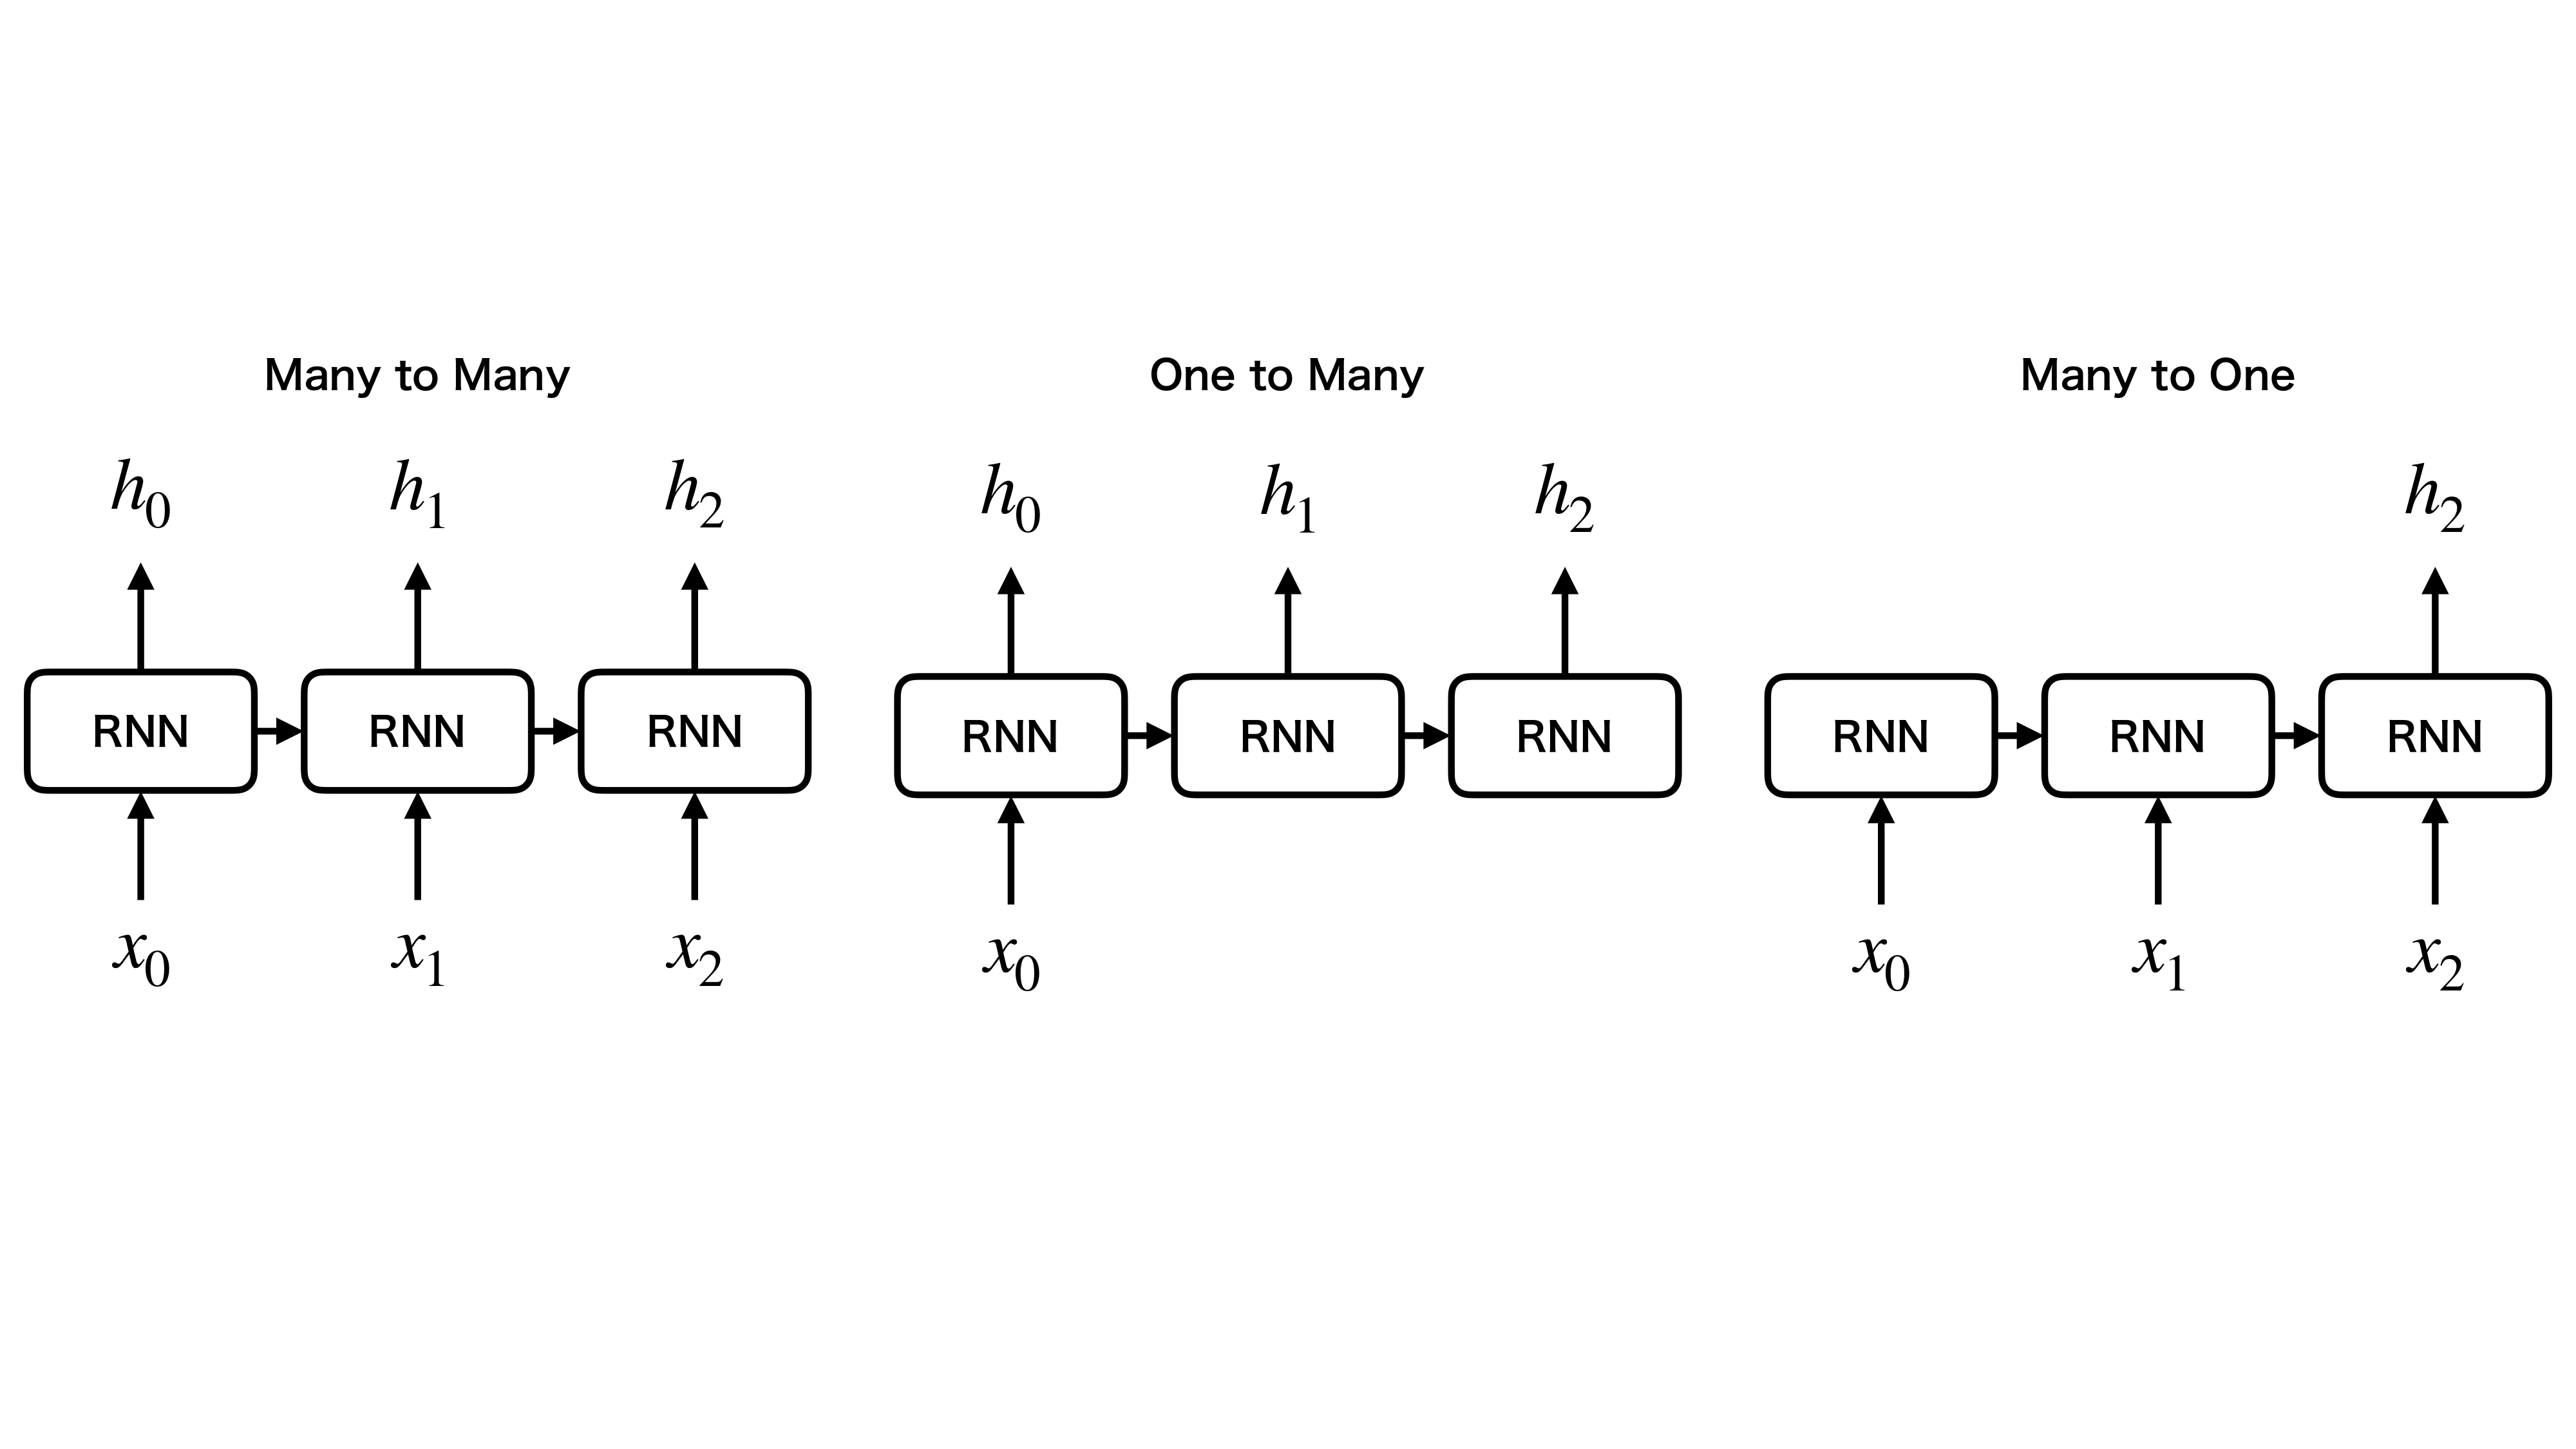
\includegraphics[trim = 0 200 0 200, width=1.0\textwidth, clip]{Figure/2DeepLearning/9RNNOutputs.png}
 \caption[リカレントニューラルネットワークの出力方法]{リカレントニューラルネットワークの出力方法}
 \label{9RNNOutputs}
\end{figure}

リカレントニューラルネットワークの学習は基本的にフィードフォワードニューラルネットワークと同様であるが, 図\ref{8RNNWeight}に見る様にネットワークは系列にしたがって深くなっている。
この為, 重み更新はこの系列を遡って行う必要がある。
このような誤差逆伝播法の事をBackpropagation Through Time (BPTT) という。
実際には計算リソースの削減のため, Truncated BPTTという, 時系列方向に適当な長さで切り取り計算を行う手法が使用される。


%%%%%%%%%%%%%%%%%%%%%%%%%%%%%%%%%%%%%%%%%%%%%%%%%%%%%%%%%%%%%%%%%%%%%%%%
\subsection{リカレントニューラルネットワークの問題点} \label{DL:RNN:IssueofRNN}

リカレントニューラルネットワークは時間方向に展開し, それを遡ることによって学習を行なっているため, 系列の長さに依存して非常に深いネットワークが構築される。
したがって, リカレントニューラルネットワークは真に深いネットワークであると言えるが, 深い層からの勾配は非常に消失あるいは爆発しやすく, 容易に勾配消失・爆発を招いてしまうという問題が生じている。
勾配消失はリカレントニューラルネットワークの活性化関数であるtanh関数に起因している。
\ref{DL:NN:TrainingofNN}項で解説したように, 誤差逆伝播法は連鎖律によって計算され, その計算には活性化関数の微分が含まれている。
ここでtanh関数の微分は, 
\begin{equation}
 \begin{split}
  \frac{\partial y(x)}{\partial x}
  &= \frac{\partial}{\partial x} \tanh(x) = \frac{1}{\cosh^2 (x)} \\
  &= 1 - \frac{\cosh^2 (x) - 1}{\cosh^2 (x)} = 1 - \frac{\sinh^2 (x)}{\cosh^2 (x)} = 1 - \tanh^2 (x) = 1 - y^2
 \end{split}
\end{equation}
と計算される。

$1-y^2$は, $y=0$以外において常に1より小さい値を取ってしまう。
リカレントニューラルネットワークでは系列長に応じて, この1より小さい値 ($1-y^2$) が複数回掛けられてしまうため, 勾配消失が生じやすくなっている。
同時にリカレントニューラルネットワークでは, 連鎖律によって系列長に応じて同じ重み行列$W_h$を複数回掛けており, この重み行列の値に応じて, 勾配が発散あるいは消失してしまうことが考えられる。

また, リカレントニューラルネットワークは時系列上の複数の入出力から, 矛盾した重み更新を受け取ってしまう入力重み衝突, 出力重み衝突という問題も抱えている。

更に, リカレントニューラルネットワークはその構造上, 長期的な系列情報を保持できないという課題も存在している。

以上のような問題を解決するため, ゲートとセルと呼ばれる技術を導入したものを, ゲート付きリカレントユニット (Gated Recurrent Unit, GRU\cite{GRU}) という。
次項では, このゲートを用いたリカレントニューラルネットワークの一つであるLSTMについて紹介する。


%%%%%%%%%%%%%%%%%%%%%%%%%%%%%%%%%%%%%%%%%%%%%%%%%%%%%%%%%%%%%%%%%%%%%%%%
\subsection{長・短期記憶 (Long Short-Term Memory, LSTM)} \label{DL:RNN:LongShortTermMemory}

LSTMのネットワーク構造全体を図\ref{10LongShortTermMemory}に示す。
リカレントニューラルネットワークとの最も大きな違いは, LSTMは隠れ状態 (出力) を二つ${\mbox{\boldmath{$h$}}}_t,{\mbox{\boldmath{$c$}}}_t$持っているという点である。
${\mbox{\boldmath{$c$}}}_t$は長期的な記憶セルを示しており, 図\ref{10LongShortTermMemory}では上部の赤い線で表現されている。
一方, ${\mbox{\boldmath{$h$}}}_t$は, リカレントニューラルネットワークと同様に短期的な系列情報の伝達と出力に使用されている。
LSTMは三つの入力${\mbox{\boldmath{$h$}}}_{t-1},{\mbox{\boldmath{$c$}}}_{t-1},{\mbox{\boldmath{$x$}}}_t$を受け取り, 二つの出力${\mbox{\boldmath{$h$}}}_t,{\mbox{\boldmath{$c$}}}_t$を提供するネットワークであるとみなすことができる。

\begin{figure}[htbp]
 \centering
 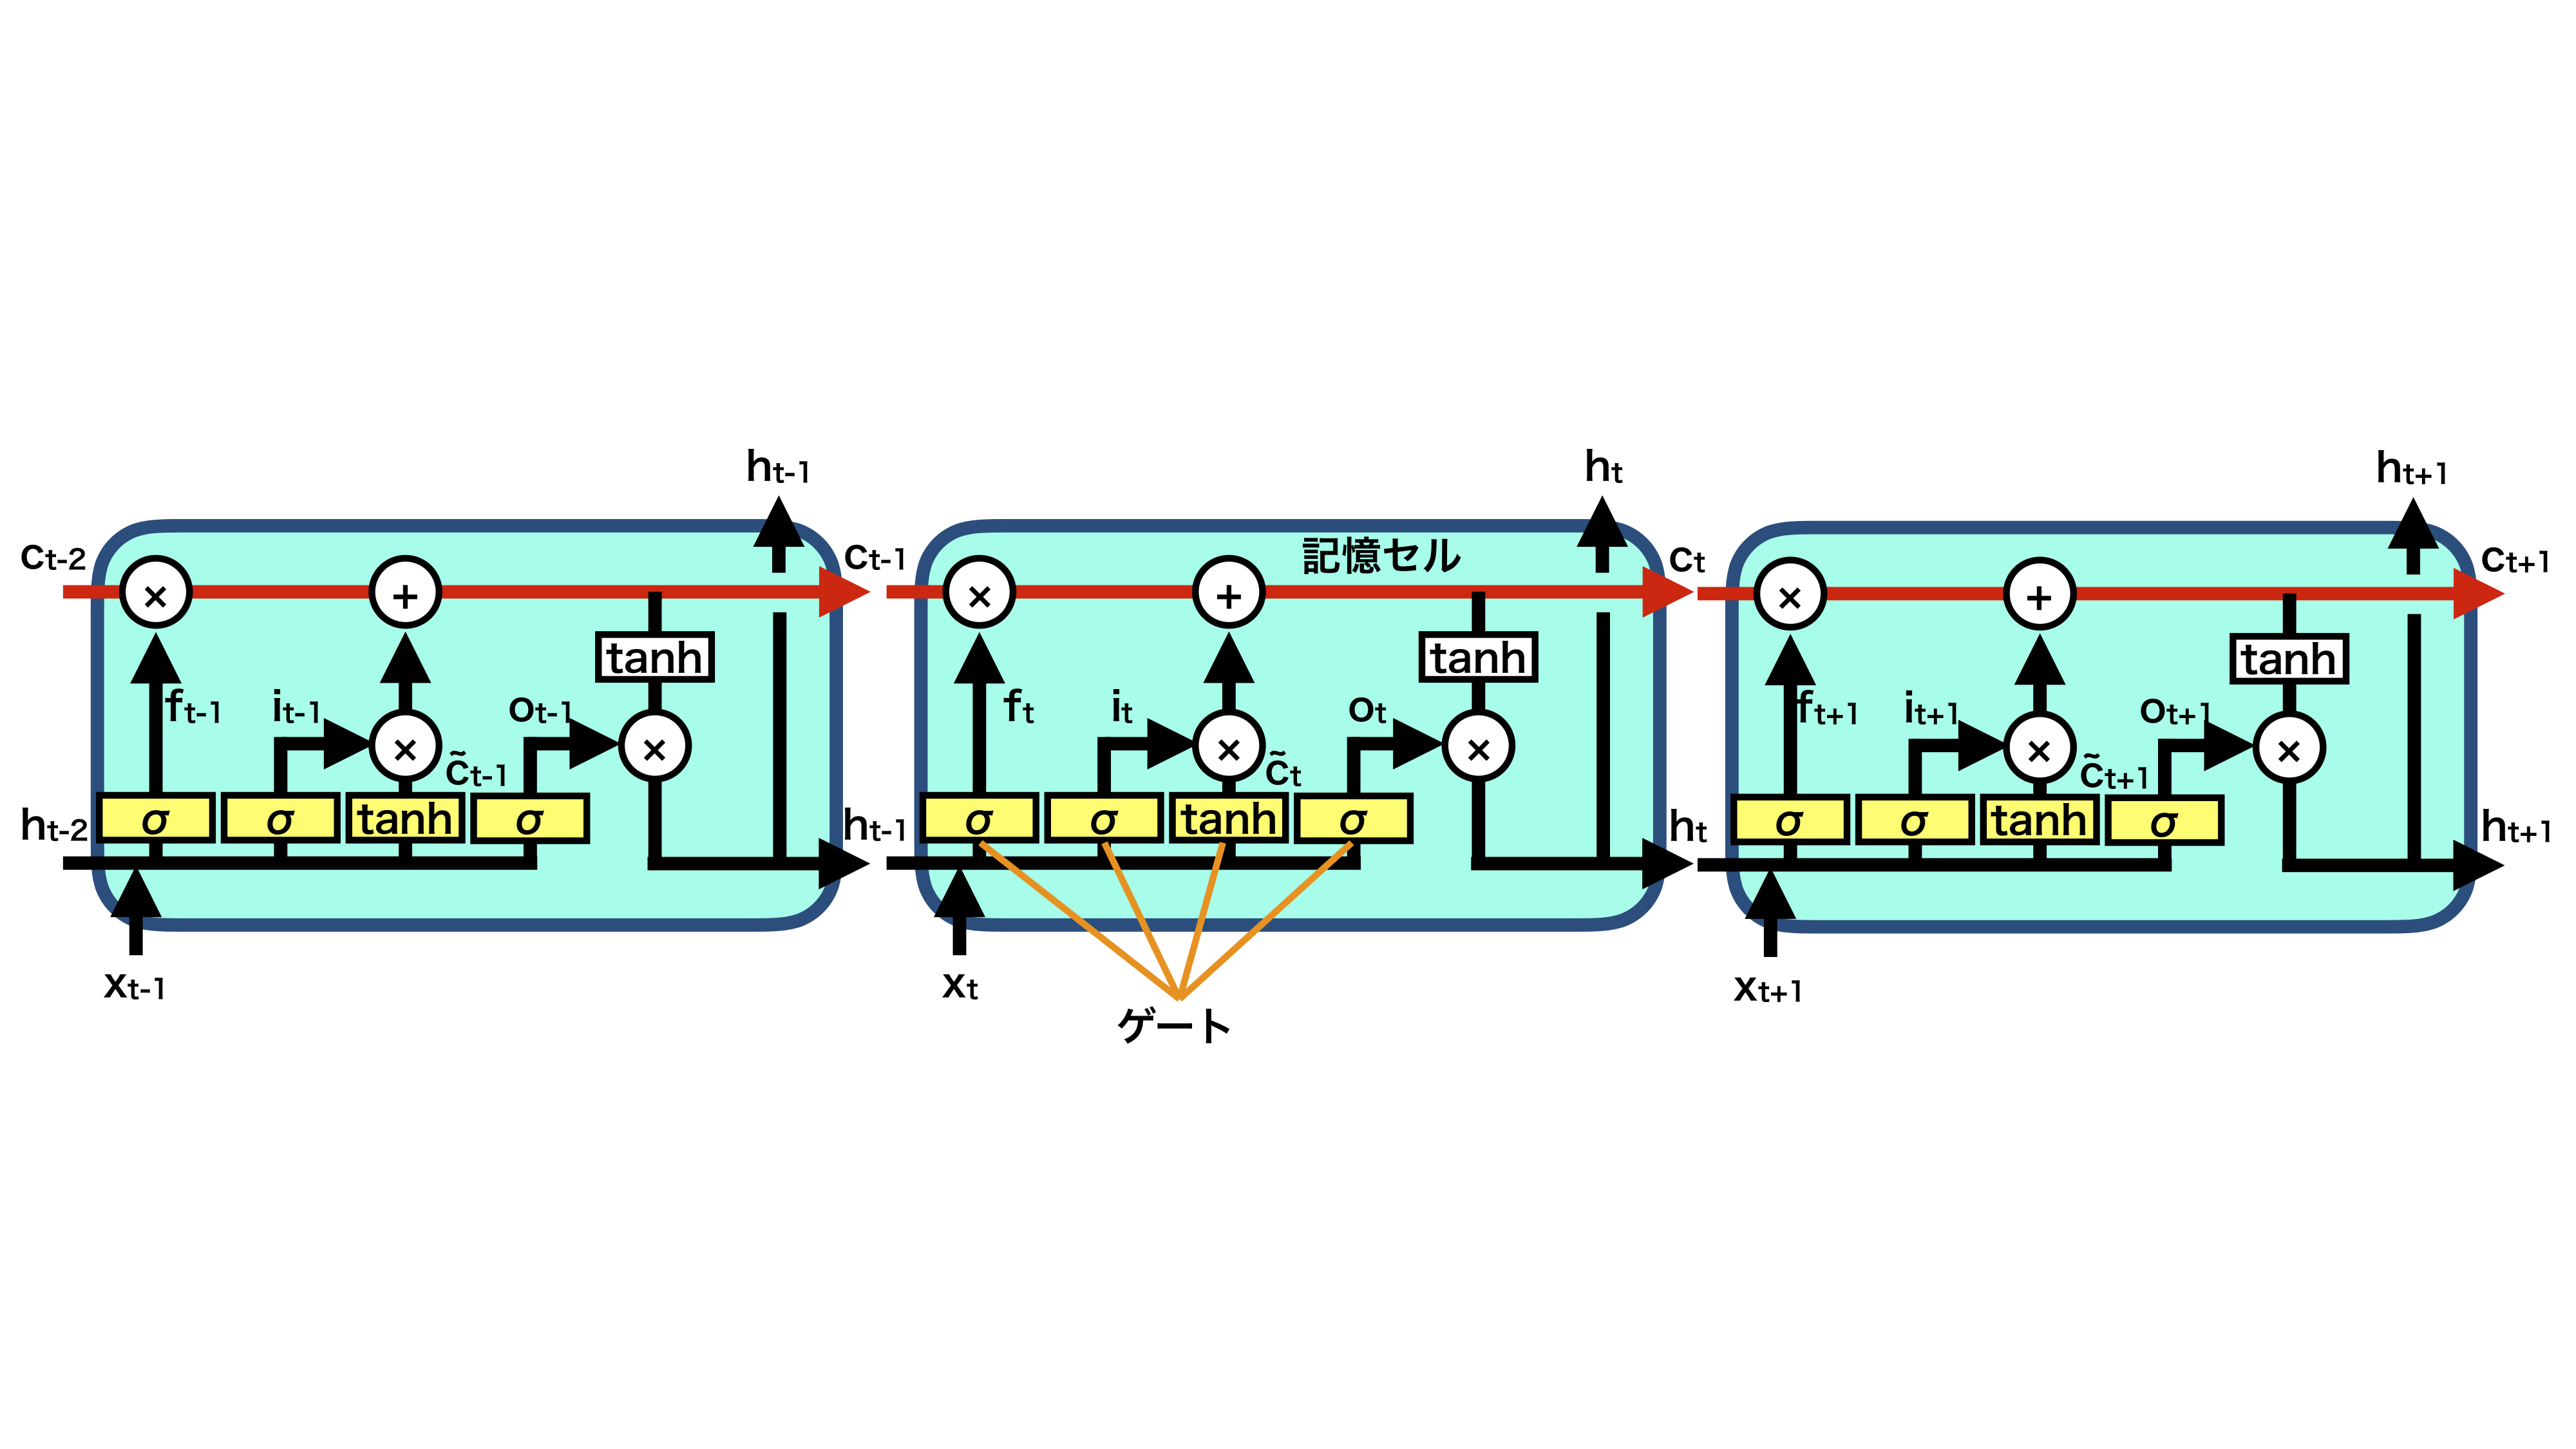
\includegraphics[trim = 0 200 0 200, width=1.0\textwidth, clip]{Figure/2DeepLearning/10LongShortTermMemory.png}
 \caption[LSTMの流れ]{LSTMの流れ。リカレントニューラルネットワークの様に時間について展開した図である。赤線が記憶セル, 黄色の各部がそれぞれゲートである。出力と隠れ状態である${\mbox{\boldmath{$h$}}},{\mbox{\boldmath{$c$}}}$は直前の系列から受け取り, 入力${\mbox{\boldmath{$x$}}}$は下方から導入されている。}
 \label{10LongShortTermMemory}
\end{figure}

また, LSTMは内部に前項で述べた勾配消失や勾配爆発, 入力重み衝突, 出力重み衝突といった様々な問題を解決するためのゲートと呼ばれる構造を四つ持っている(図\ref{10LongShortTermMemory})。

%\begin{comment}
\begin{figure}[htbp]
 \centering
 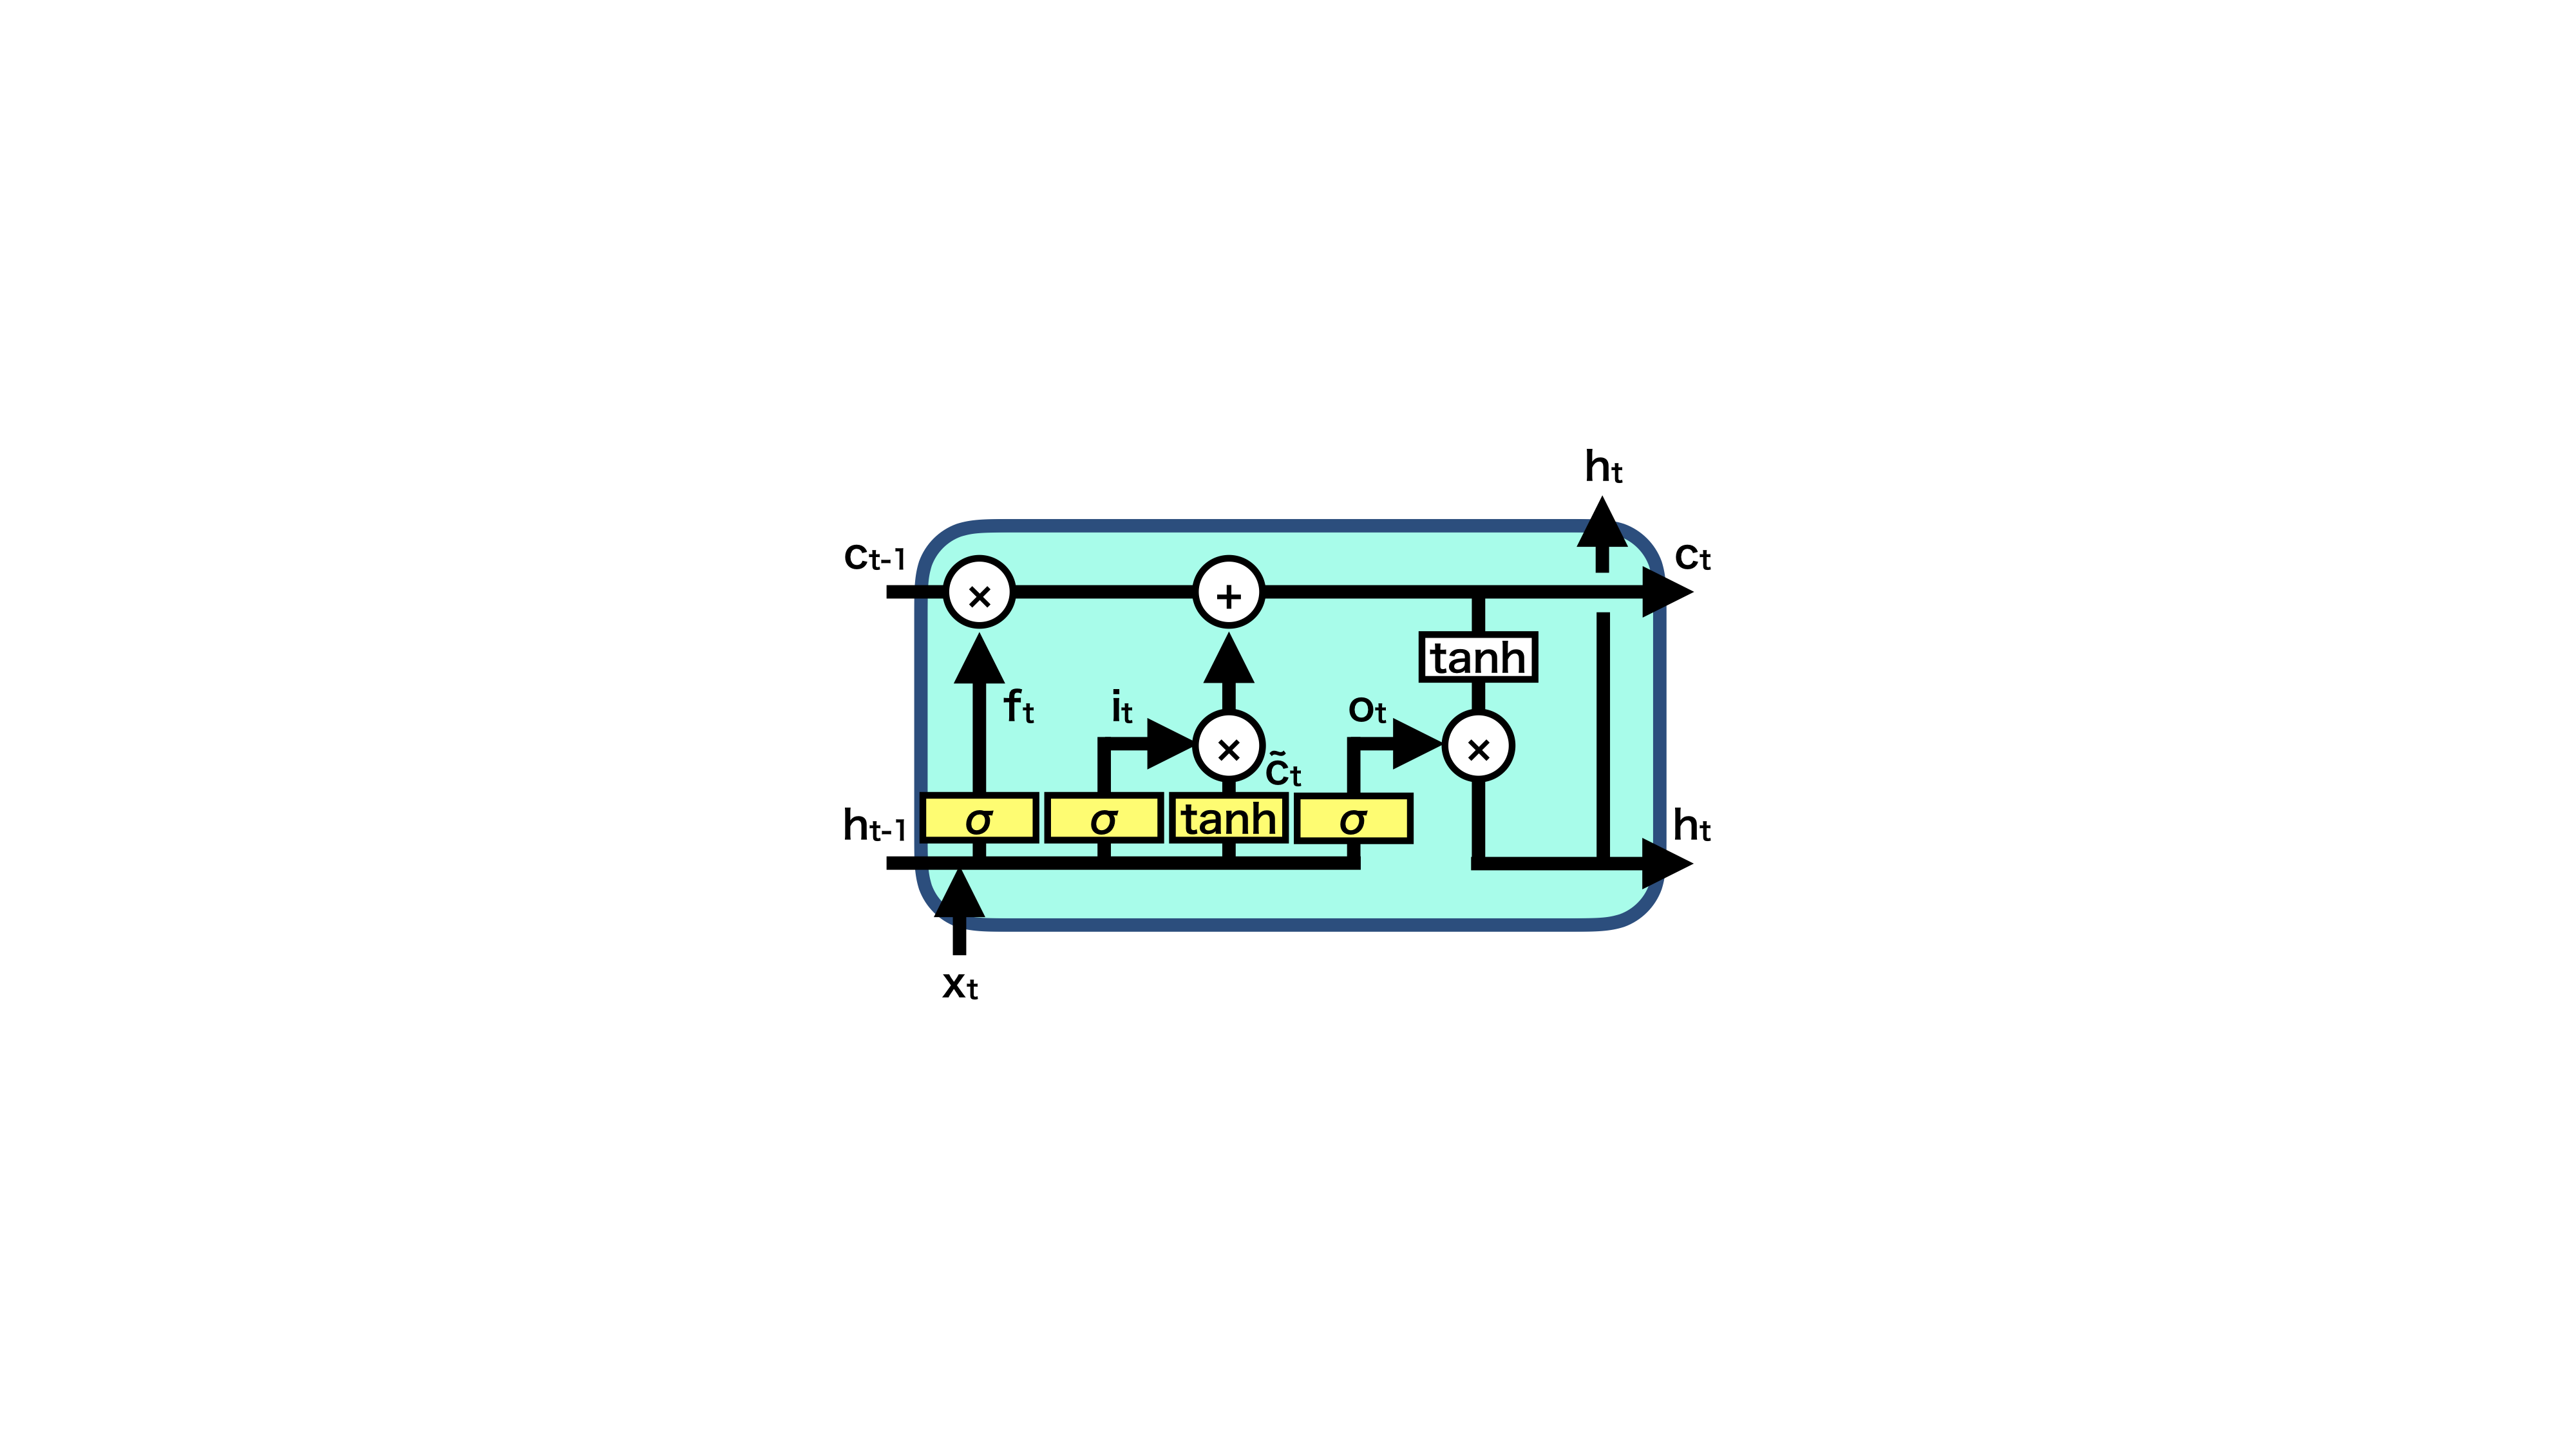
\includegraphics[trim = 0 300 0 300, width=1.0\textwidth, clip]{Figure/2DeepLearning/11LSTM.png}
 \caption[単体のLSTM]{単体のLSTM。系列$1$ステップ分のLSTMを切り出したものである。リカレントニューラルネットワークと同様に重み行列は各ステップに渡って同一のものが使用されている。}
 \label{11LSTM}
\end{figure}
%\end{comment}

四つのゲートはそれぞれ忘却ゲート, 入力ゲート, セルの更新, 出力ゲートと呼ばれている。
入力ゲート, 出力ゲートはそれぞれ重み衝突を回避するために導入されており, 忘却ゲート, セルの更新は長期記憶の適切な長期記憶セルの更新を行う為のアイデアである。
それぞれの役割と演算を以下にまとめる。

\begin{itemize}
  \item 忘却ゲート\\
  図\ref{12ForgetGate}の赤い線で表現している領域では, 入力${\mbox{\boldmath{$h$}}}_{t-1},{\mbox{\boldmath{$x$}}}_t$を用いて, どの程度, 直前の長期記憶セル${\mbox{\boldmath{$c$}}}_{t-1}$を忘れるかの度合いである${\mbox{\boldmath{$f$}}}_{t}$を計算している。
  ${\mbox{\boldmath{$f$}}}_{t}$は, 次のようにかける。
\begin{equation}
 \begin{split}
  {\mbox{\boldmath{$f$}}}_{t} = \sigma (W_f {\mbox{\boldmath{$x$}}}_t + R_f {\mbox{\boldmath{$h$}}}_{t-1})
 \end{split}
\end{equation}  
  したがって最終的には, 
\begin{equation}
 \begin{split}
  {\mbox{\boldmath{$c$}}}_{t-1} \  {\mbox{\boldmath{$f$}}}_{t} 
  = {\mbox{\boldmath{$c$}}}_{t-1} \  \sigma (W_f {\mbox{\boldmath{$x$}}}_t + R_f {\mbox{\boldmath{$h$}}}_{t-1})
 \end{split}
\end{equation}
  として, 次のゲート以降で長期記憶を更新するための容量を確保していると解釈できる。

  \item 入力ゲート\\
  入力ゲートは忘却ゲートと全く同じ構造 (図\ref{13InputGate}) をしており, 次のように計算できる。
\begin{equation}
 \begin{split}
  {\mbox{\boldmath{$i$}}}_{t} = \sigma (W_i {\mbox{\boldmath{$x$}}}_t + R_i {\mbox{\boldmath{$h$}}}_{t-1})
 \end{split}
\end{equation}
  忘却ゲートではどの程度, 長期記憶セルを忘れるかを計算していたように, 入力ゲートでの${\mbox{\boldmath{$i$}}}_{t}$は, 次のセルの更新時に新しい長期記憶セルをどの程度重視するかを表現していると解釈できる。
    
  \item セルの更新\\
  図\ref{14CellUpdate}では, まず更新された長期記憶セル$\tilde{{\mbox{\boldmath{$c$}}}}_t$を計算している。
\begin{equation}
 \begin{split}
  \tilde{{\mbox{\boldmath{$c$}}}}_t = \tanh (W_c {\mbox{\boldmath{$x$}}}_t + R_c {\mbox{\boldmath{$h$}}}_{t-1})
 \end{split}
\end{equation} 
  次にこれまでの三つのゲートの結果をまとめることで, 新しい隠れ状態である長期記憶セル${\mbox{\boldmath{$c$}}}_{t}$を計算できる。
\begin{equation}
 \begin{split}
  {\mbox{\boldmath{$c$}}}_{t} 
  &= {\mbox{\boldmath{$c$}}}_{t-1} \  {\mbox{\boldmath{$f$}}}_{t} + \tilde{\mbox{\boldmath{$c$}}}_{t}\ {\mbox{\boldmath{$i$}}}_{t}\\
  &= {\mbox{\boldmath{$c$}}}_{t-1} \  \sigma (W_f {\mbox{\boldmath{$x$}}}_t + R_f {\mbox{\boldmath{$h$}}}_{t-1}) 
  + \tanh (W_c {\mbox{\boldmath{$x$}}}_t + R_c {\mbox{\boldmath{$h$}}}_{t-1}) \  \sigma (W_i {\mbox{\boldmath{$x$}}}_t + R_i {\mbox{\boldmath{$h$}}}_{t-1})
 \end{split}
\end{equation}
  第一項では, 直前の長期記憶セル${\mbox{\boldmath{$c$}}}_{t-1}$をどの程度忘れるかを${\mbox{\boldmath{$f$}}}_{t}$によって制御し, 第二項では, 新しく計算された長期記憶セル$\tilde{\mbox{\boldmath{$c$}}}_{t}$をどの程度重視するかを${\mbox{\boldmath{$i$}}}_{t}$によって制御している。
    
  \item 出力ゲート\\
  出力ゲートでは, ここまでで計算された${\mbox{\boldmath{$c$}}}_{t}$と入力${\mbox{\boldmath{$x$}}}_t, {\mbox{\boldmath{$h$}}}_{t-1}$を用いて, 最終的な出力となる${\mbox{\boldmath{$h$}}}_{t}$を計算している。
  ただし, 出力ゲート${\mbox{\boldmath{$o$}}}_{t}$自体は入力ゲートや忘却ゲートと全く同じ形 (図\ref{15OutputGate}) をしている。
  具体的な計算は次のように書ける。
\begin{equation}
 \begin{split}
  {\mbox{\boldmath{$o$}}}_{t} 
  &= \sigma (W_o {\mbox{\boldmath{$x$}}}_t + R_o {\mbox{\boldmath{$h$}}}_{t-1})\\
  {\mbox{\boldmath{$h$}}}_{t} 
  &= \tanh({\mbox{\boldmath{$c$}}}_{t}) \  {\mbox{\boldmath{$o$}}}_{t}\\
  &= \tanh({\mbox{\boldmath{$c$}}}_{t}) \  \sigma (W_o {\mbox{\boldmath{$x$}}}_t + R_o {\mbox{\boldmath{$h$}}}_{t-1})\\
  &= \tanh({\mbox{\boldmath{$c$}}}_{t-1} \  \sigma (W_f {\mbox{\boldmath{$x$}}}_t + R_f {\mbox{\boldmath{$h$}}}_{t-1}) 
  + \tanh (W_c {\mbox{\boldmath{$x$}}}_t + R_c {\mbox{\boldmath{$h$}}}_{t-1}) \  \sigma (W_i {\mbox{\boldmath{$x$}}}_t + R_i {\mbox{\boldmath{$h$}}}_{t-1})) \\
  &\  \sigma (W_o {\mbox{\boldmath{$x$}}}_t + R_o {\mbox{\boldmath{$h$}}}_{t-1})
 \end{split}
\end{equation}
\end{itemize}

\begin{figure}[htbp]
 \centering
  %\begin{tabular}{cccc}
  \begin{minipage}{1.0\textwidth}
  \centering
   \begin{minipage}{0.48\textwidth}
    \centering
    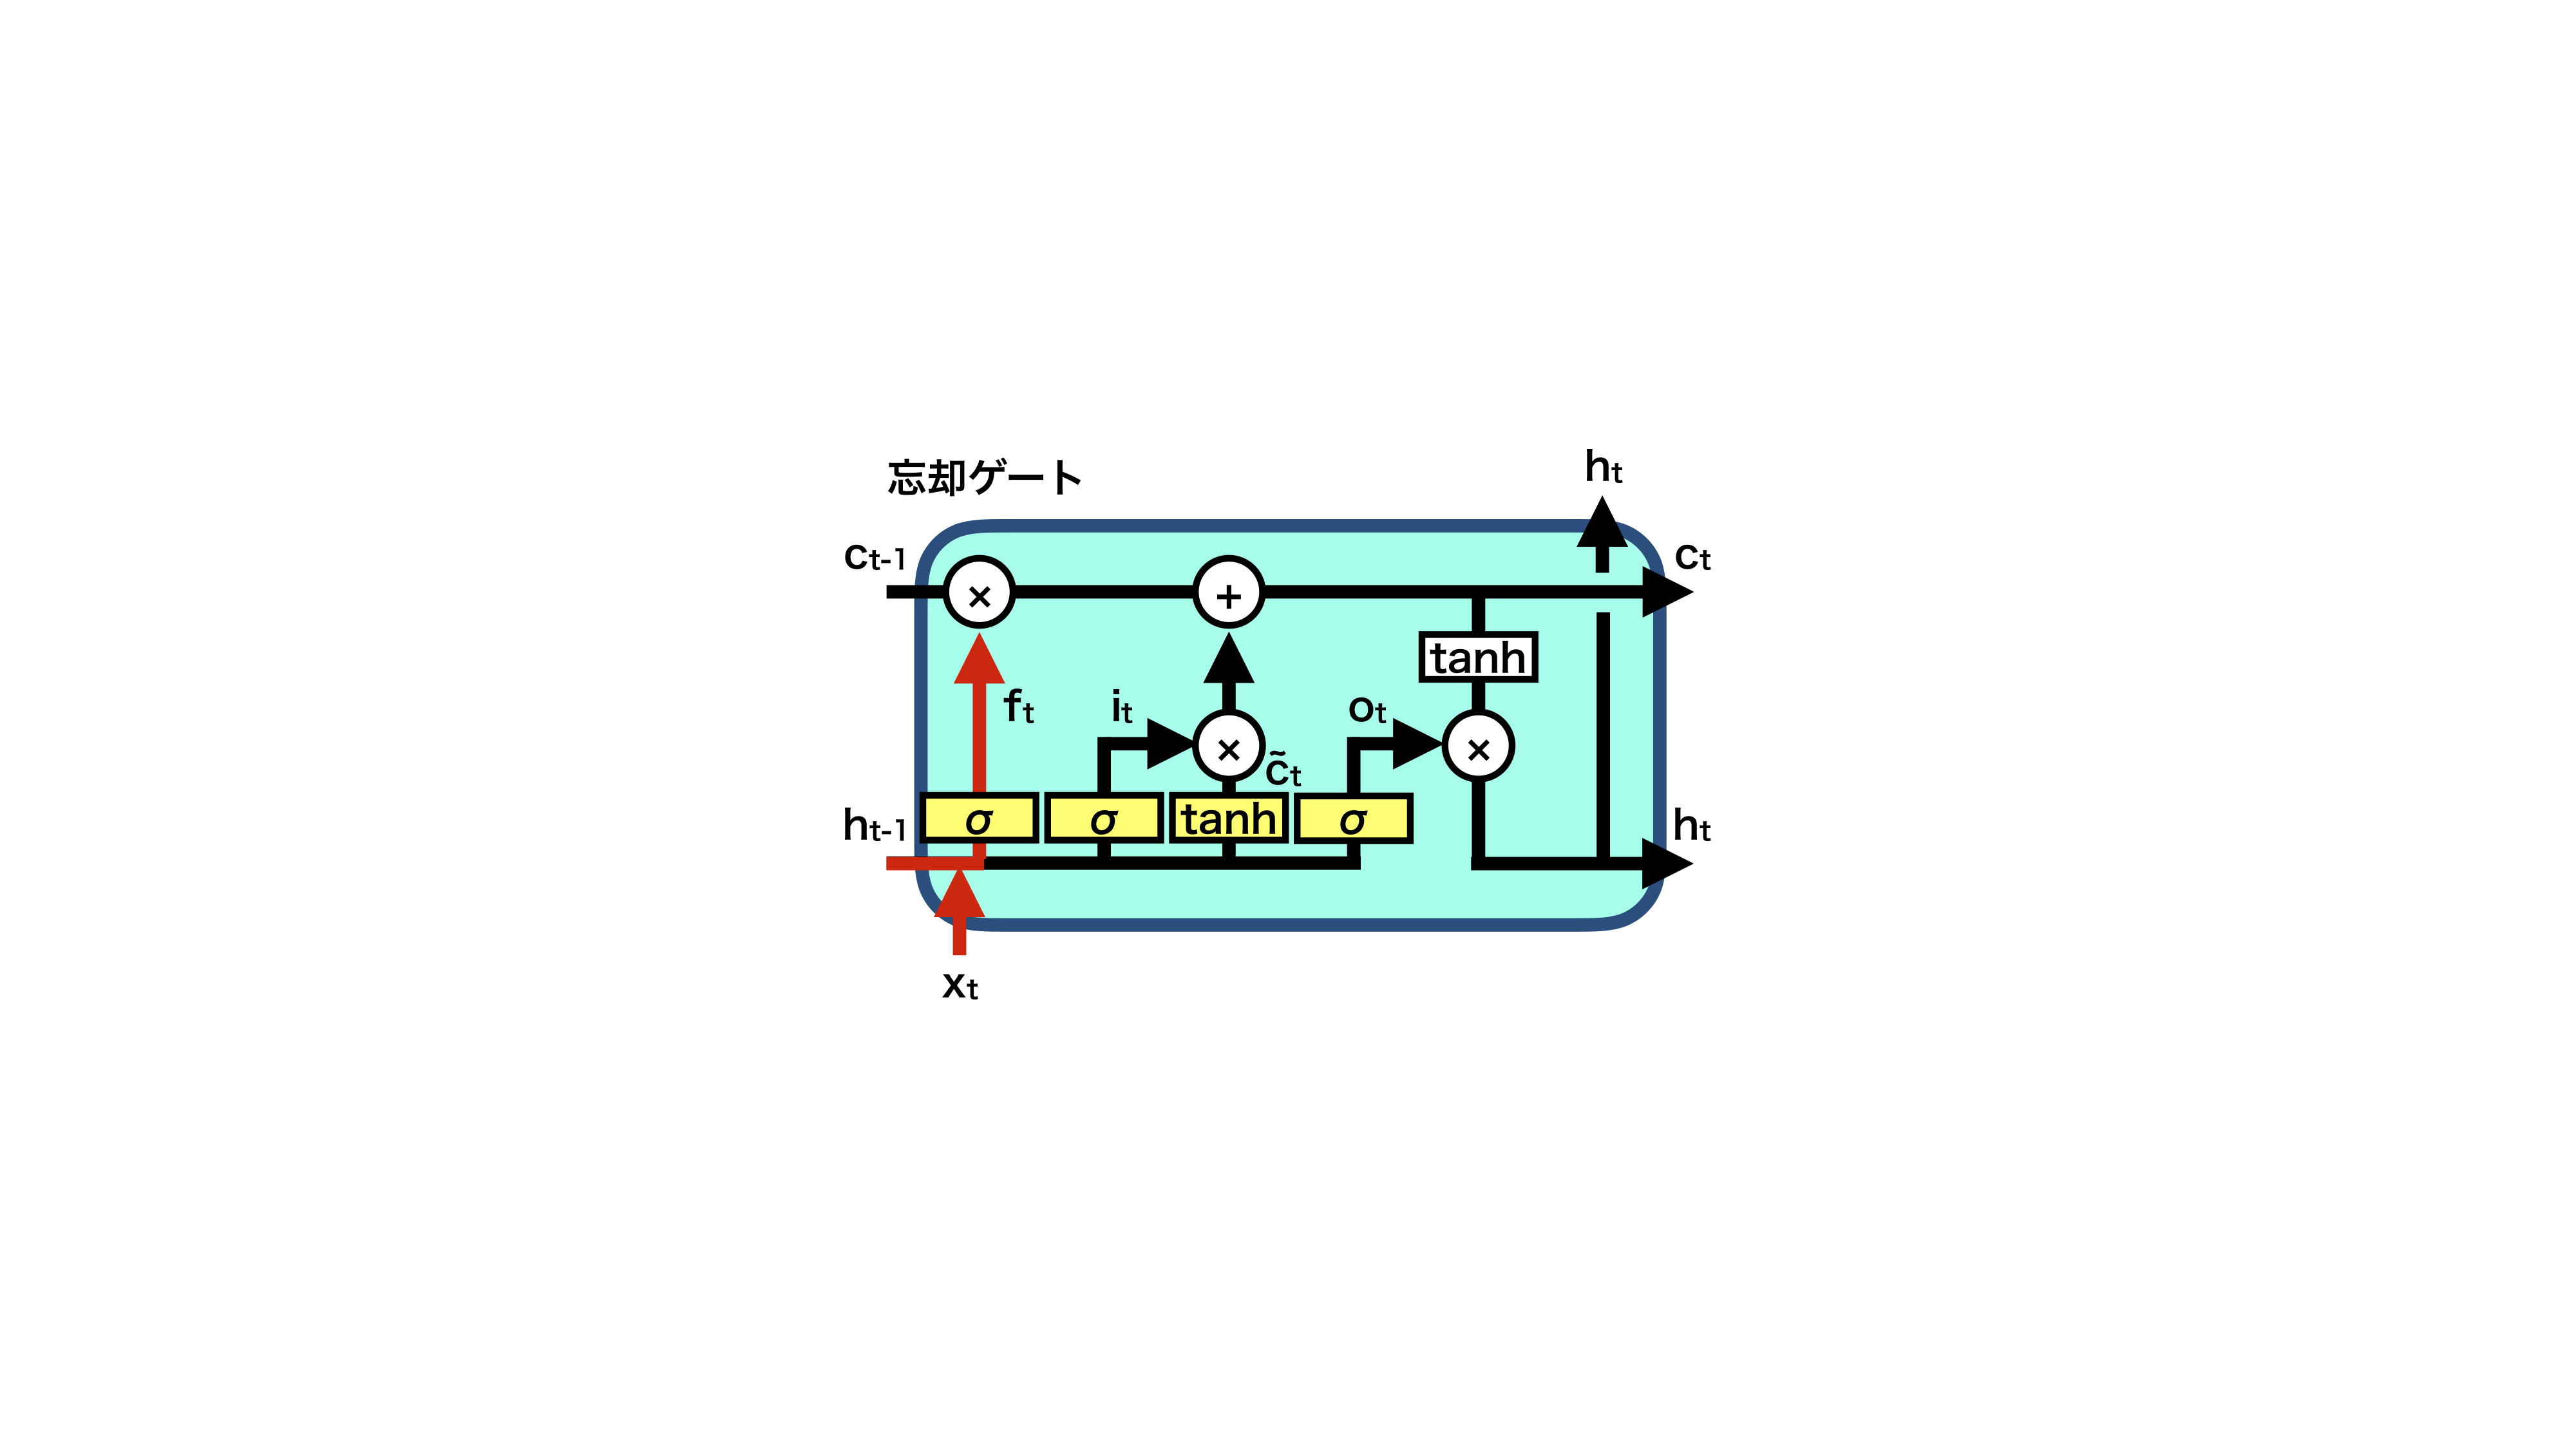
\includegraphics[trim = 600 300 600 300, width=0.9\textwidth, clip]{Figure/2DeepLearning/12ForgetGate.png}
    \subcaption{忘却ゲート}
    \label{12ForgetGate}
   \end{minipage}
   \begin{minipage}{0.48\textwidth}
   \centering
    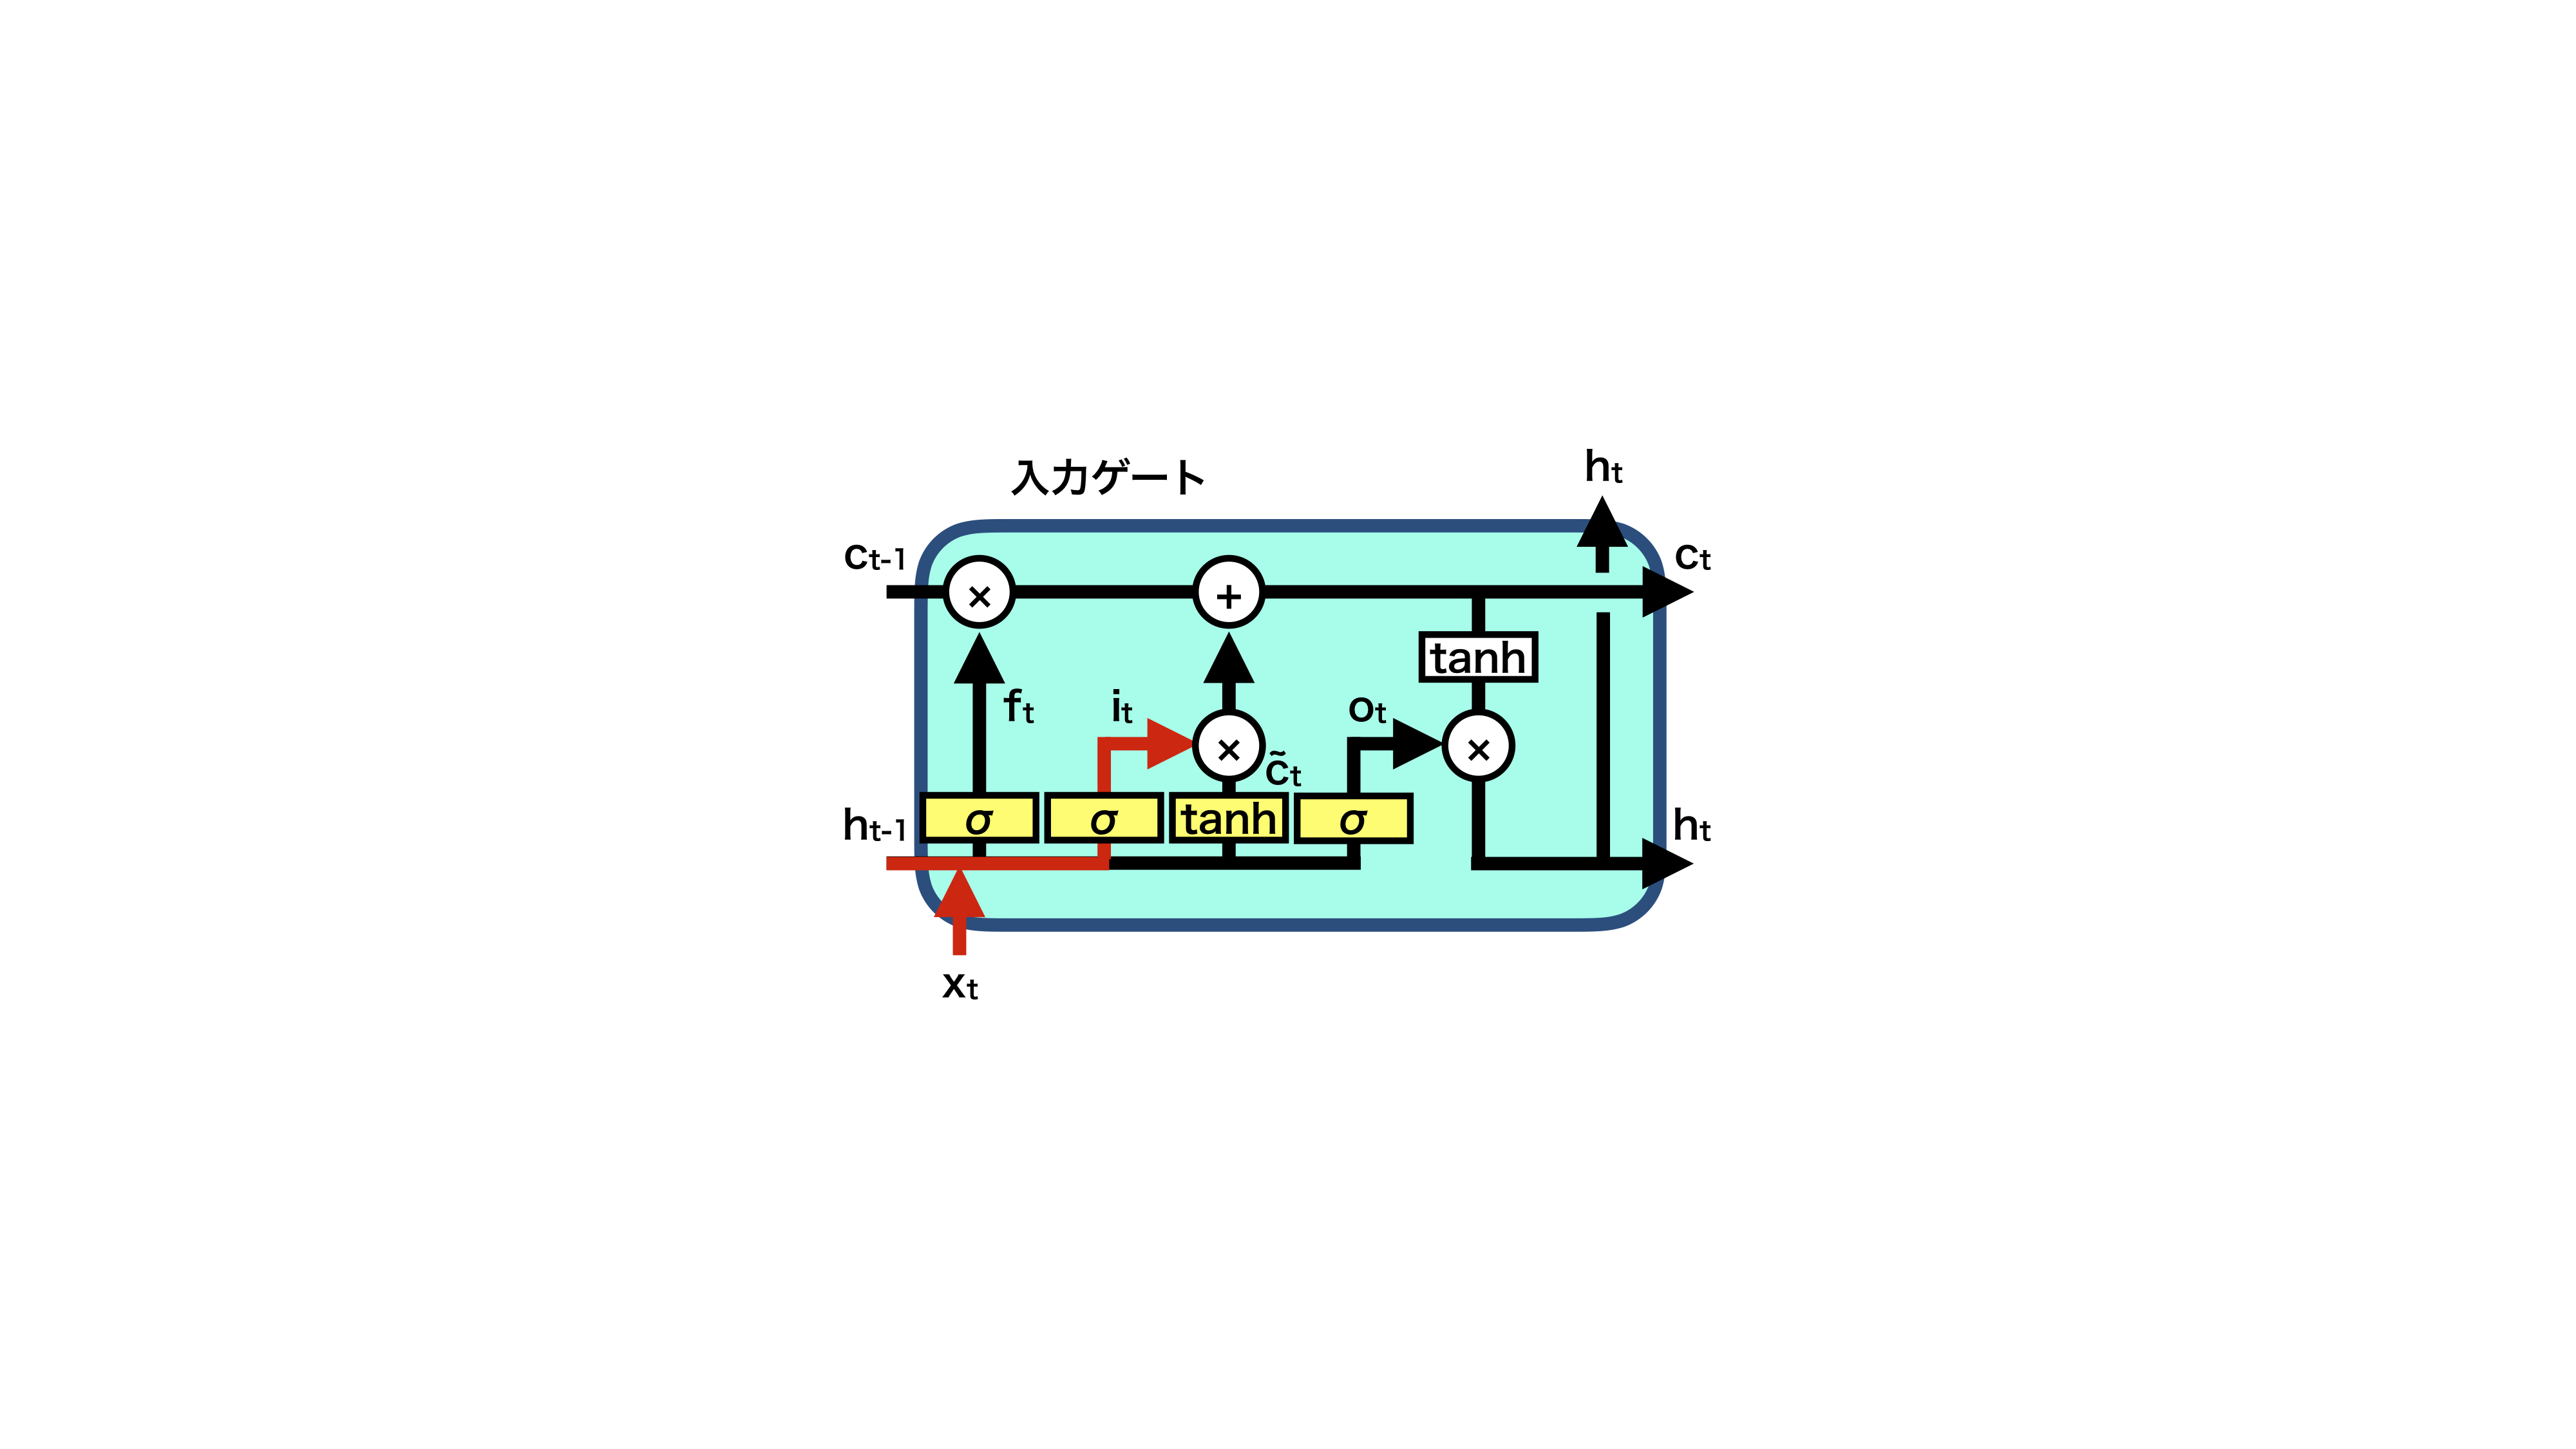
\includegraphics[trim = 600 300 600 300, width=0.9\textwidth, clip]{Figure/2DeepLearning/13InputGate.png}
    \subcaption{入力ゲート}
    \label{13InputGate}
   \end{minipage}
  \end{minipage}
  
  \begin{minipage}{1.0\textwidth}
  \centering
   \begin{minipage}{0.48\textwidth}
   \centering
    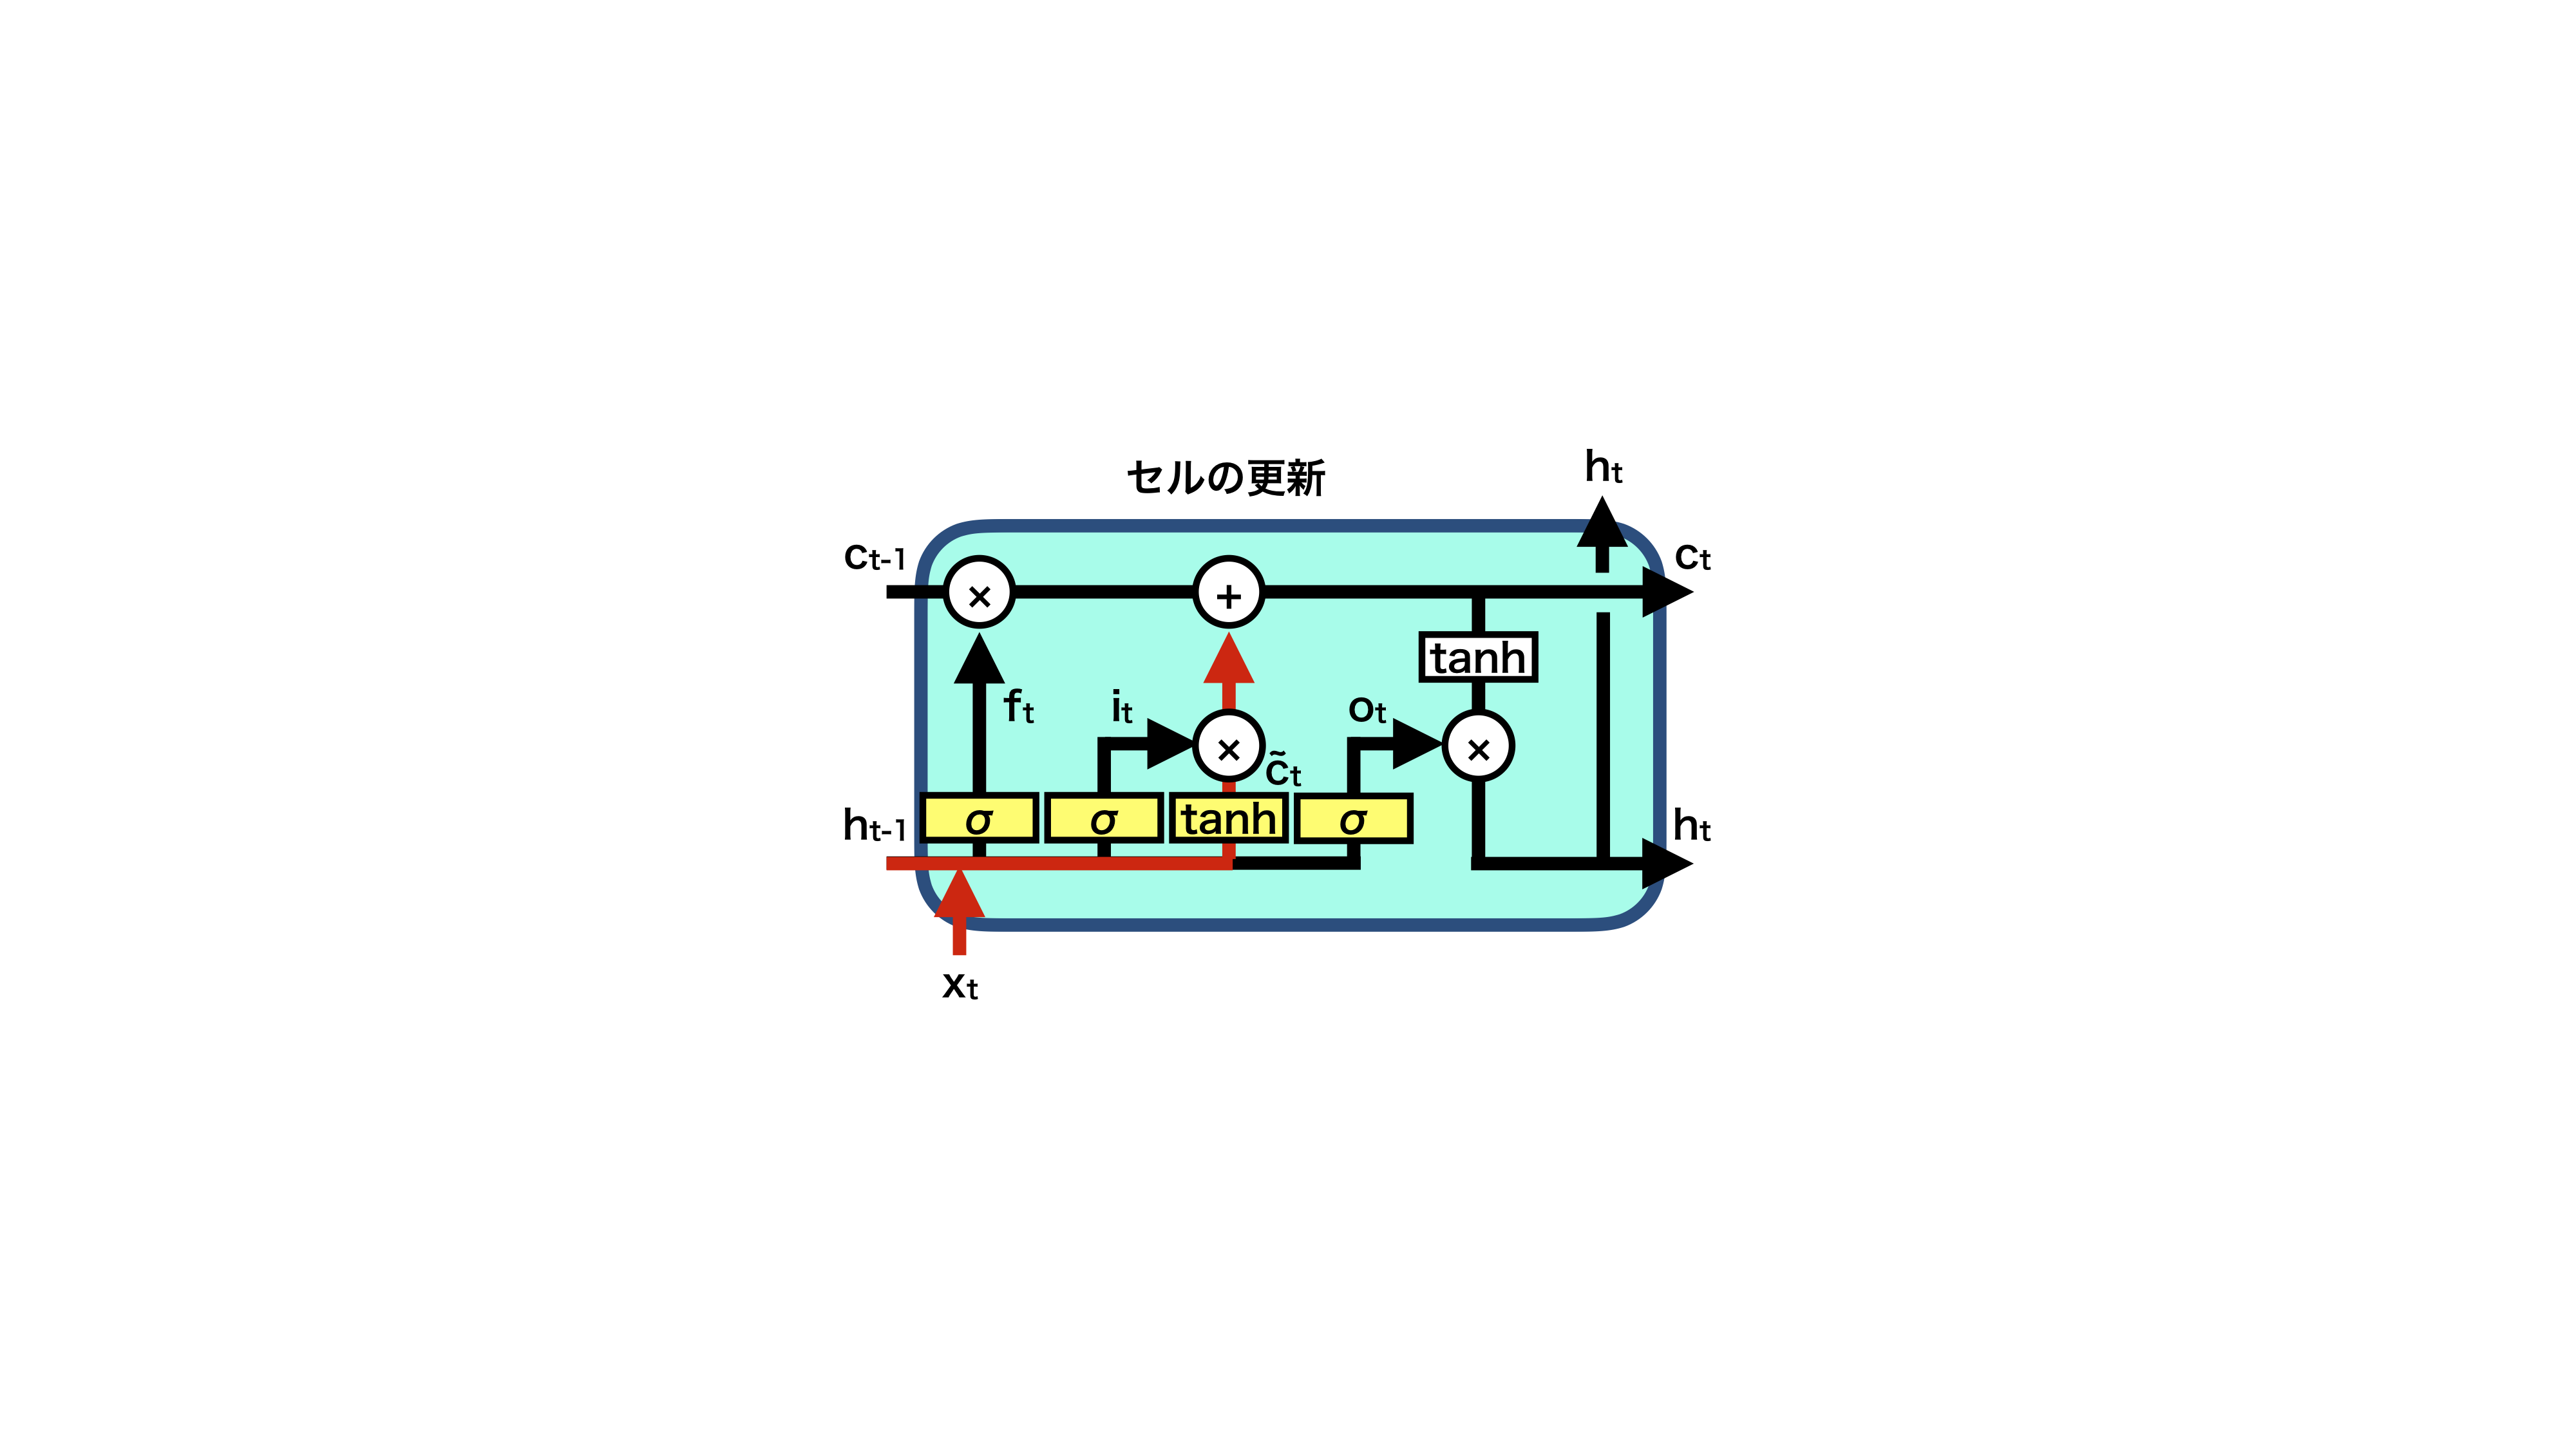
\includegraphics[trim = 600 300 600 300, width=0.9\textwidth, clip]{Figure/2DeepLearning/14CellUpdate.png}
    \subcaption{セルの更新}
    \label{14CellUpdate}
   \end{minipage}
   \begin{minipage}{0.48\textwidth}
   \centering
    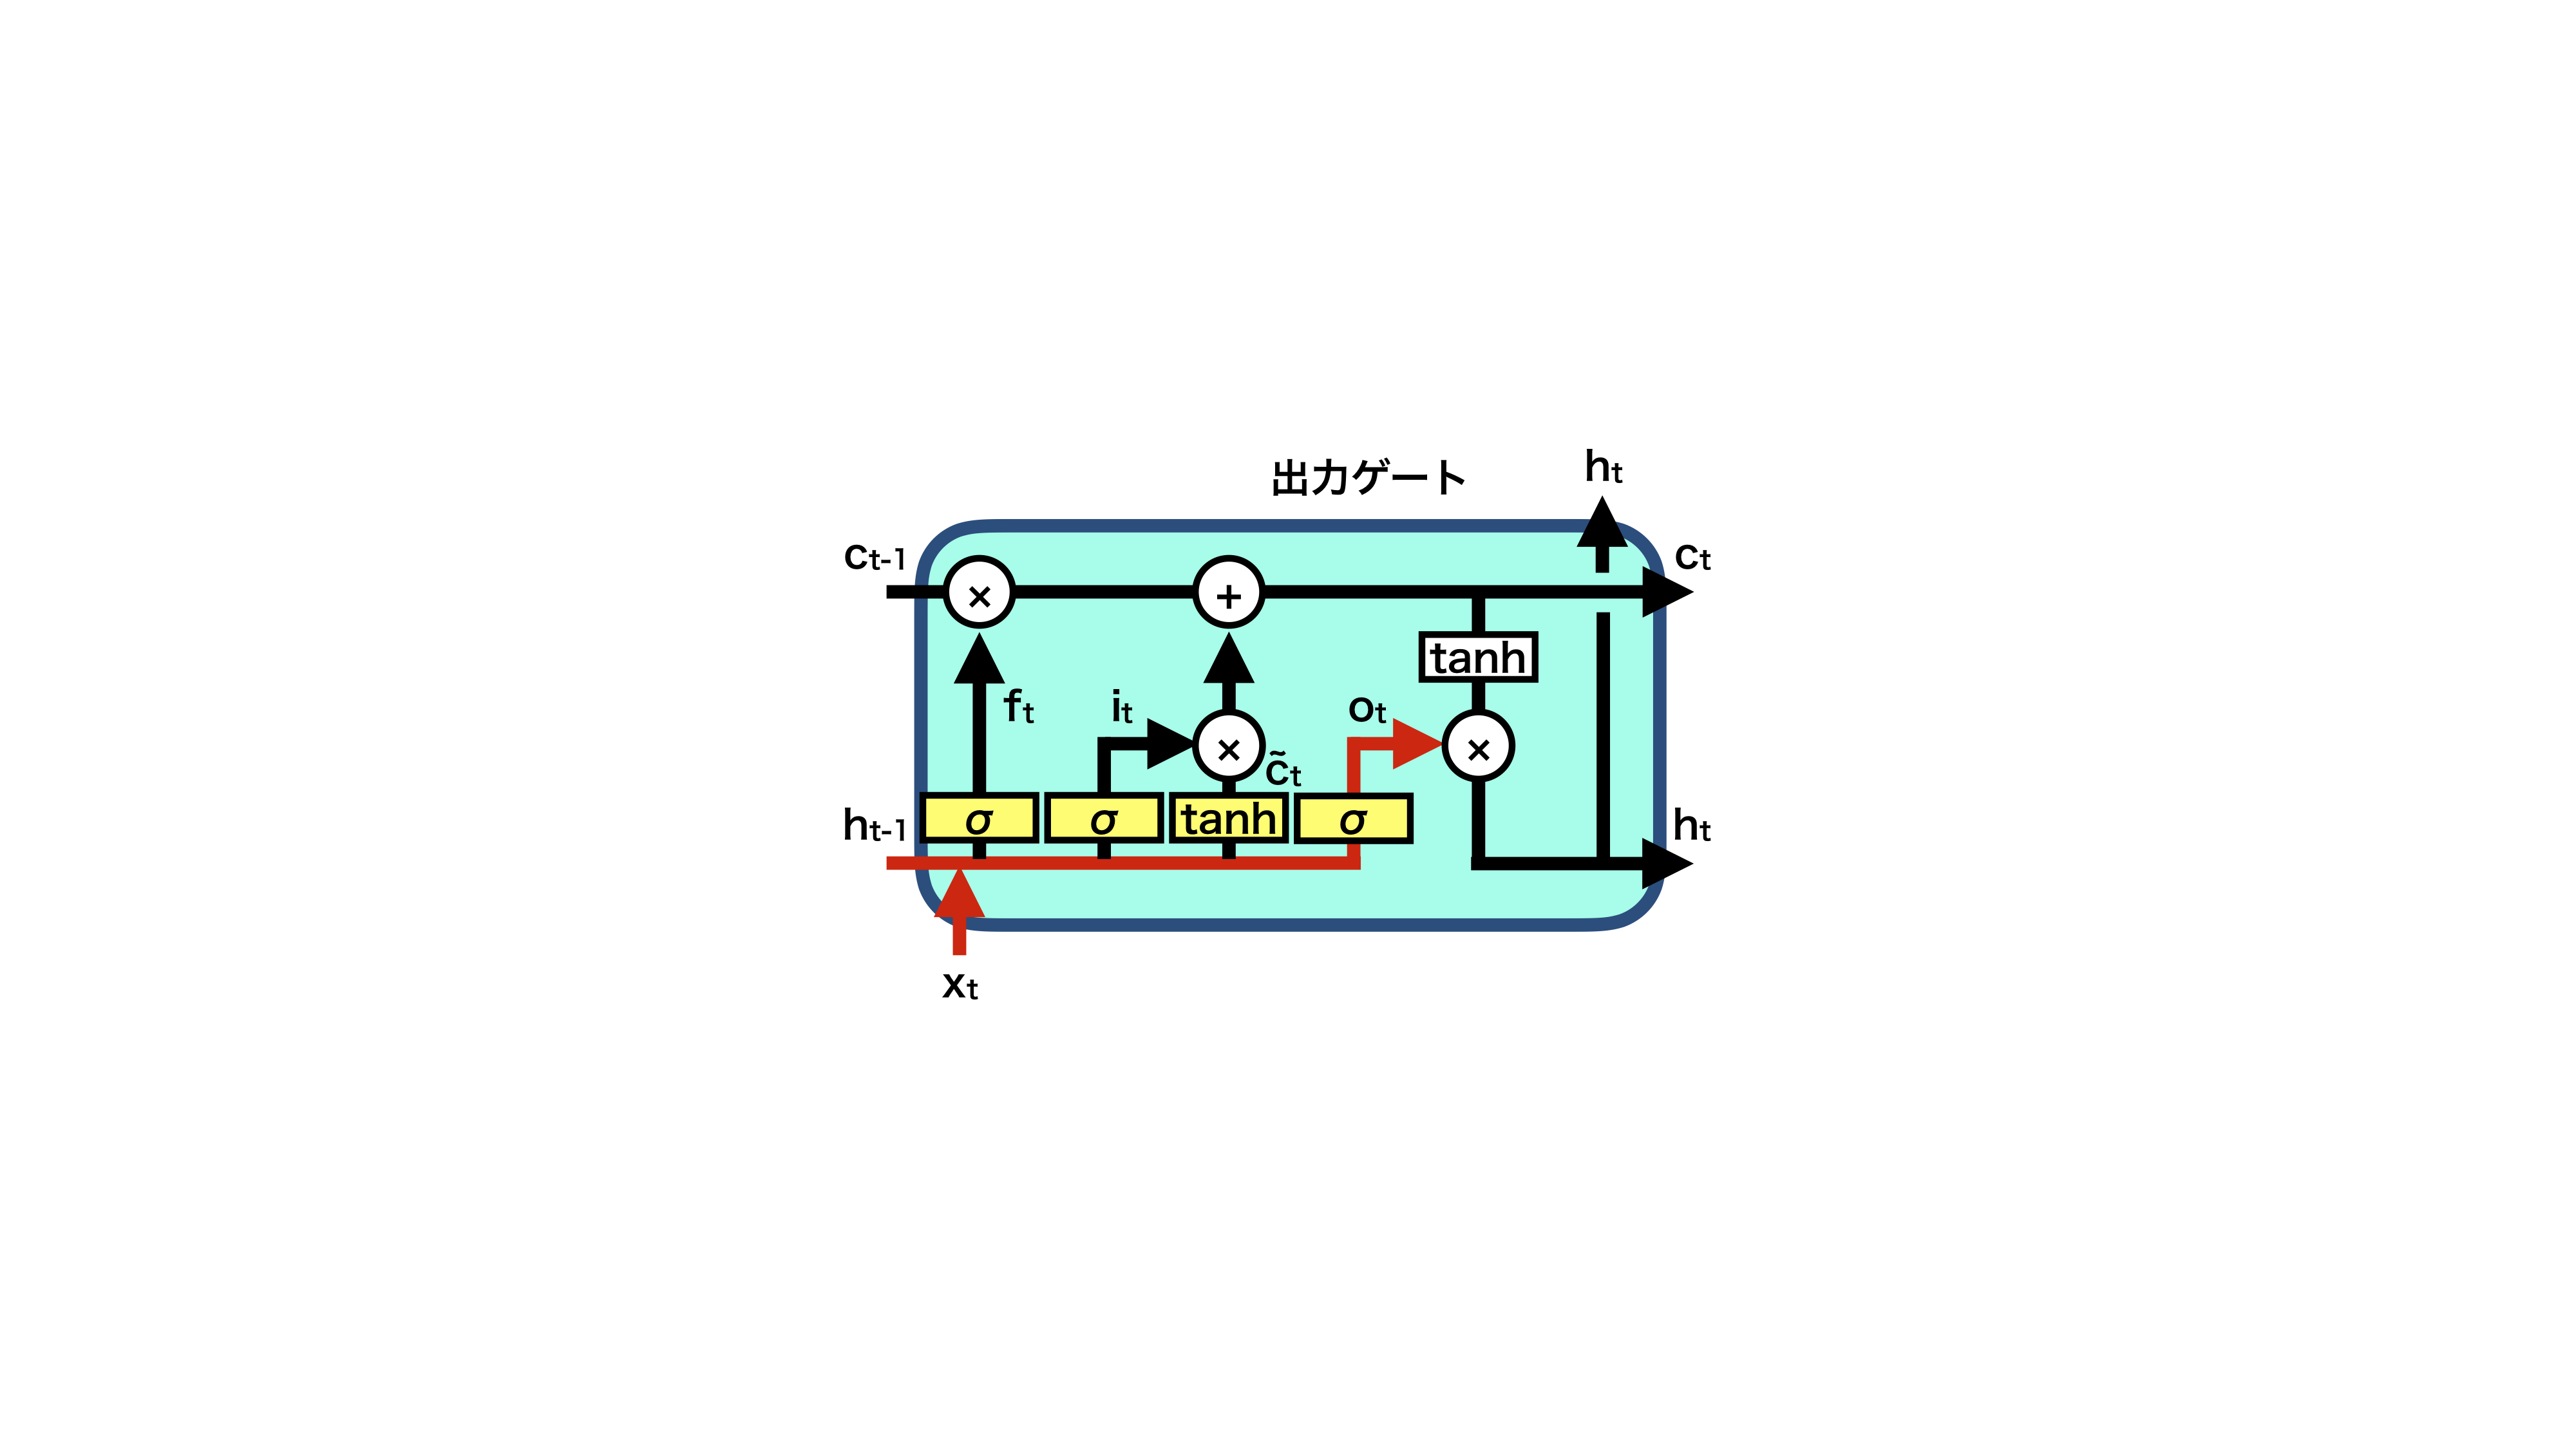
\includegraphics[trim = 600 300 600 300, width=0.9\textwidth, clip]{Figure/2DeepLearning/15OutputGate.png}
    \subcaption{出力ゲート}
    \label{15OutputGate}
   \end{minipage}
   \end{minipage}
  \caption[LSTMの各ゲートについての図解]{LSTMの各ゲートについての図解。それぞれ赤線部に沿って情報が伝達される。}
 %\end{tabular}
\end{figure}

以上のように, LSTMの内部構造は煩雑であるが, その構成要素は全てリカレントニューラルネットワークと同様に全結合で計算できる。
以下に最終的な出力の計算についてまとめる。
\begin{equation}
 \begin{split}
  {\mbox{\boldmath{$c$}}}_{t} 
  &= {\mbox{\boldmath{$c$}}}_{t-1} \  \sigma (W_f {\mbox{\boldmath{$x$}}}_t + R_f {\mbox{\boldmath{$h$}}}_{t-1}) 
  + \tanh (W_c {\mbox{\boldmath{$x$}}}_t + R_c {\mbox{\boldmath{$h$}}}_{t-1}) \  \sigma (W_i {\mbox{\boldmath{$x$}}}_t + R_i {\mbox{\boldmath{$h$}}}_{t-1})\\
  {\mbox{\boldmath{$h$}}}_{t} 
  &= \tanh({\mbox{\boldmath{$c$}}}_{t-1} \  \sigma (W_f {\mbox{\boldmath{$x$}}}_t + R_f {\mbox{\boldmath{$h$}}}_{t-1}) 
  + \tanh (W_c {\mbox{\boldmath{$x$}}}_t + R_c {\mbox{\boldmath{$h$}}}_{t-1}) \  \sigma (W_i {\mbox{\boldmath{$x$}}}_t + R_i {\mbox{\boldmath{$h$}}}_{t-1})) \\
  &\  \sigma (W_o {\mbox{\boldmath{$x$}}}_t + R_o {\mbox{\boldmath{$h$}}}_{t-1})
 \end{split}
\end{equation}

ここで, 隠れ状態 (出力) ${\mbox{\boldmath{$h$}}}_t,{\mbox{\boldmath{$c$}}}_t$の計算は全て入力${\mbox{\boldmath{$h$}}}_{t-1},{\mbox{\boldmath{$c$}}}_{t-1},{\mbox{\boldmath{$x$}}}_t$によって計算できている。
また, 学習可能な重み行列は$W_f, W_i, W_c, W_o, R_f, R_i, R_c, R_o$の八つである。
一般に, 適宜バイアス$b$が加えられる。

リカレントニューラルネットワークやLSTMは更に重ねられる (Stacked) という非常に強力な性質を持っている。
そのようなネットワークを図\ref{16StackedLSTM}に示す。
図からわかるように, 一段目のLSTMの出力が二段目のLSTMの入力になっている。
一方で, セルは両者で共有されず, 独立した状態を保持している。
それら以外の基本的な構造は一段であった時のLSTMと変わっていない。
このように, LSTMは系列としての深さだけでなく, フィードフォワードニューラルネットワークと同様に重ねることによる深さの確保が可能である。
勿論この重ねる操作は二段以上への拡張が可能であり, その場合は二段目の出力を三段目の入力に使うことによって実現できる。
どの程度重ねるかはハイパーパラメータである。

\begin{figure}[htbp]
 \centering
 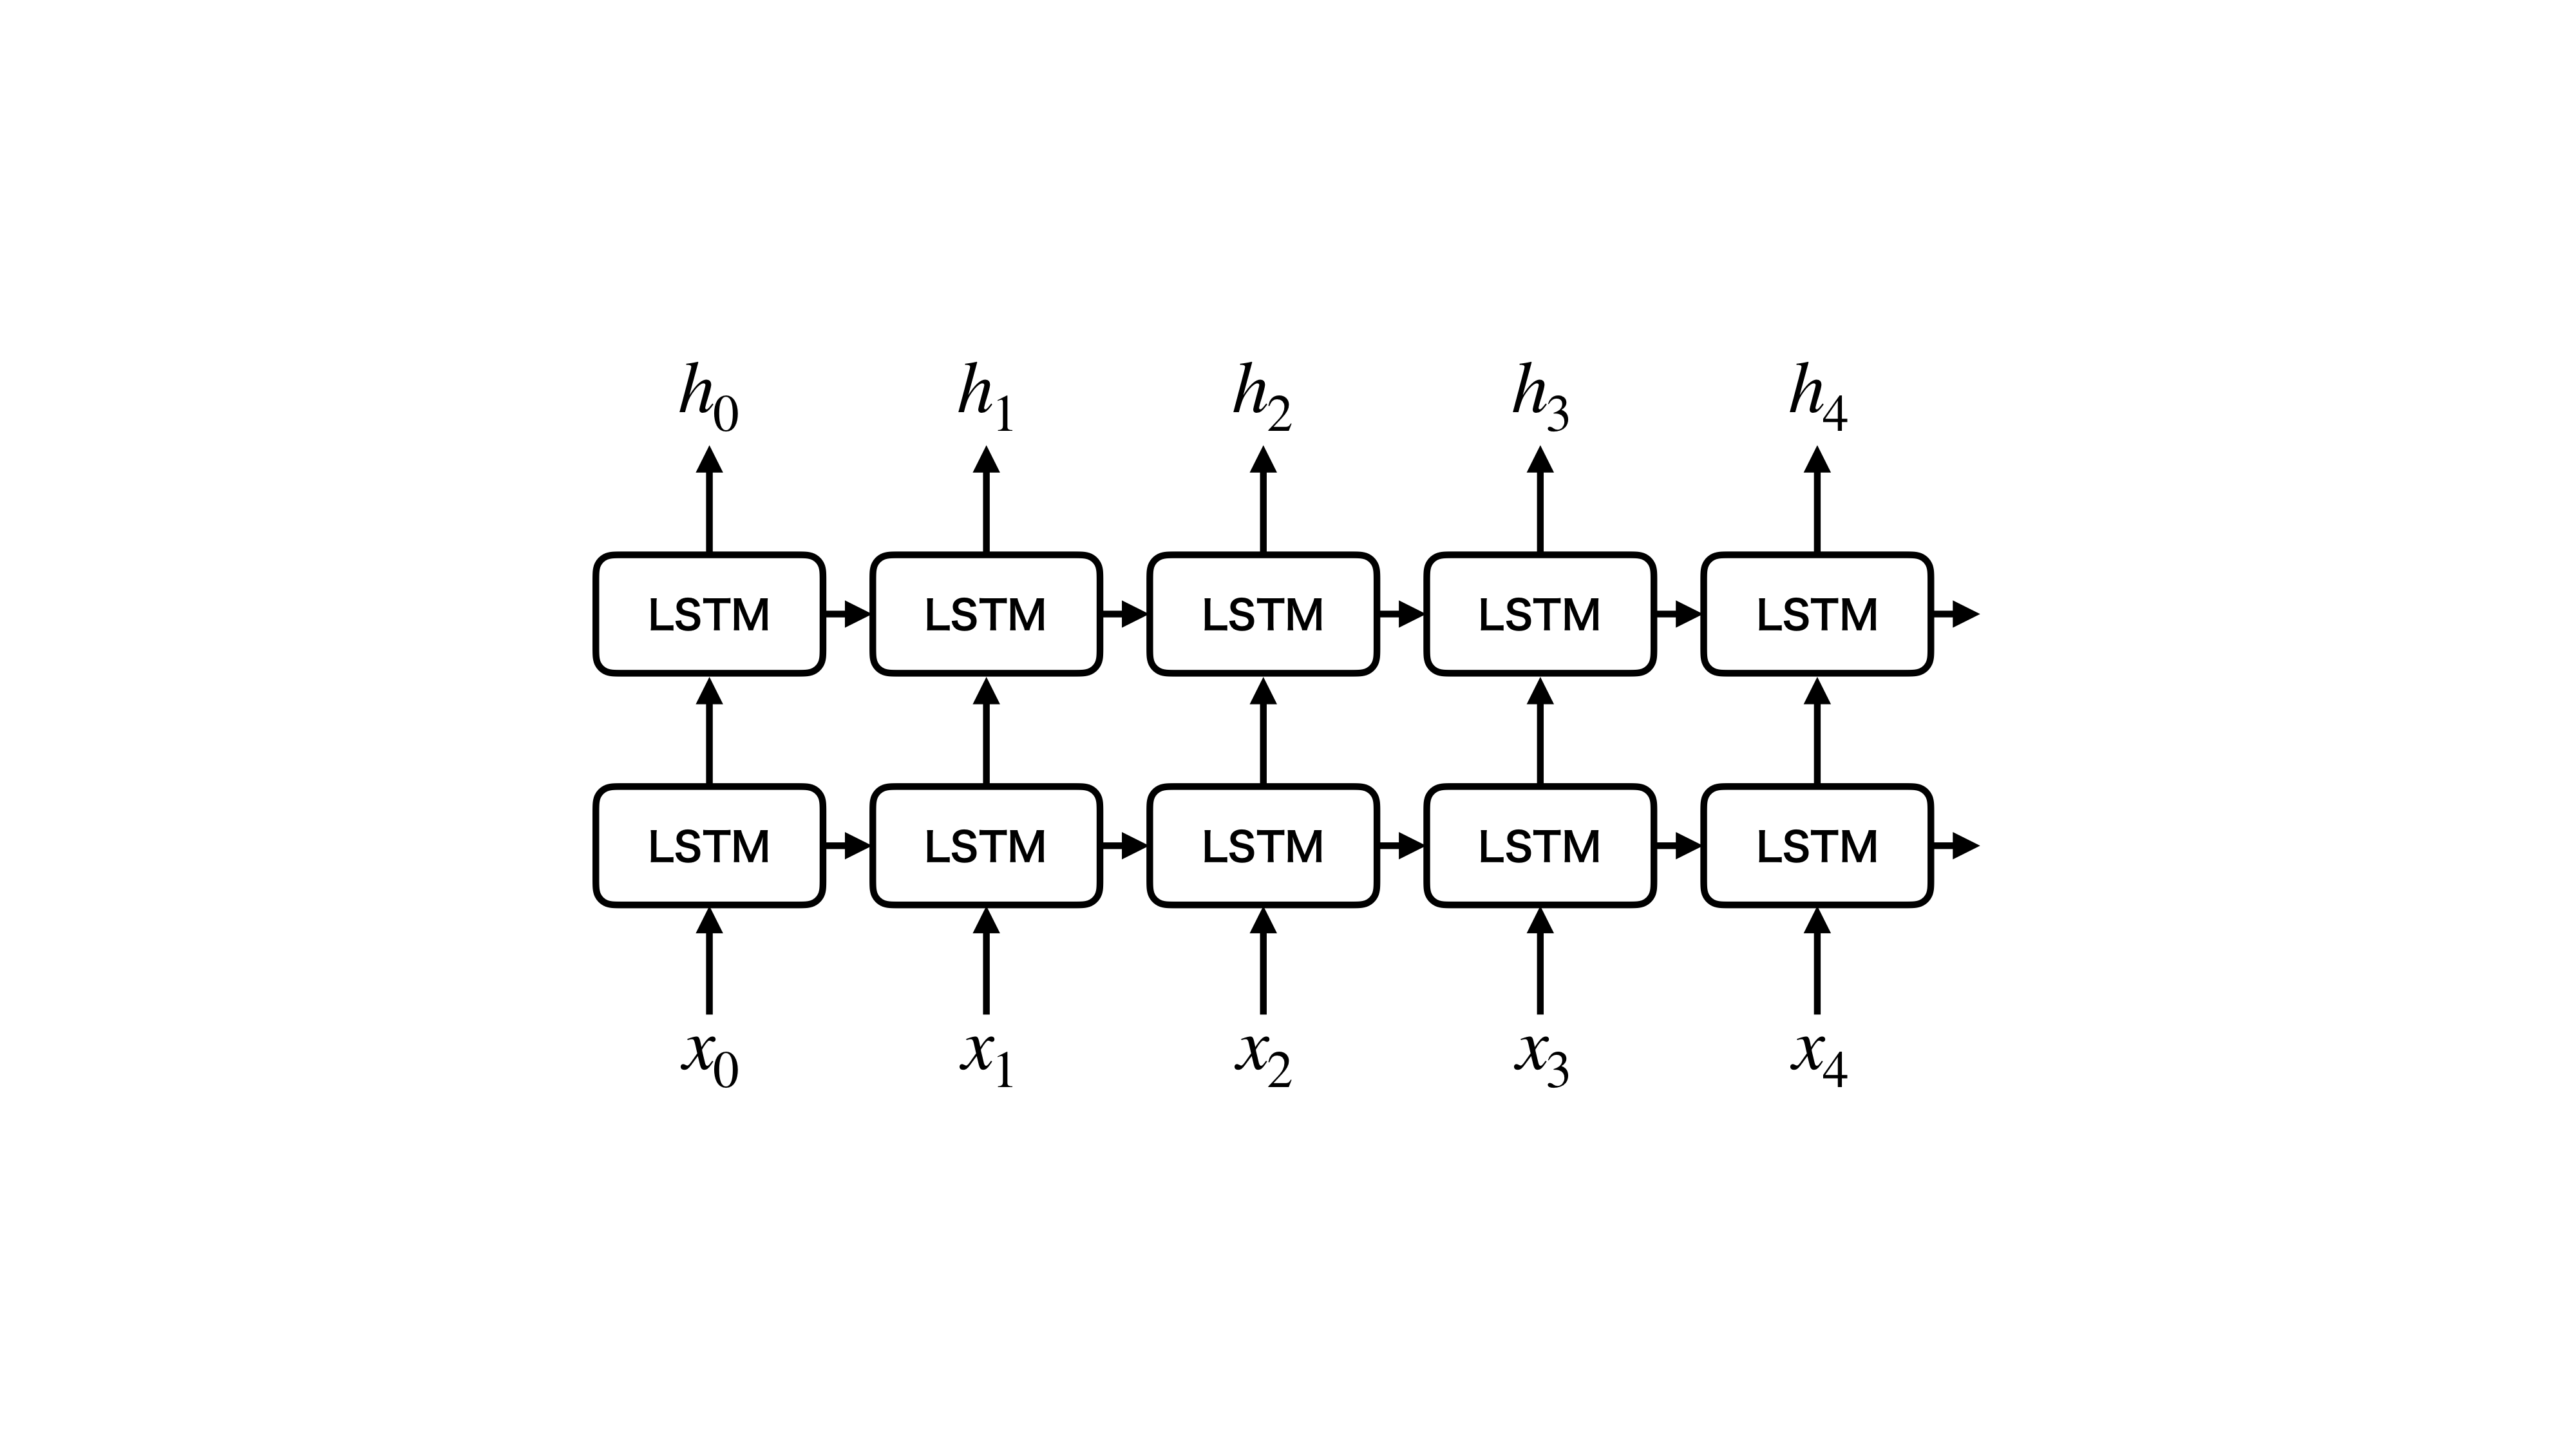
\includegraphics[trim = 0 200 0 200, width=1.0\textwidth, clip]{Figure/2DeepLearning/16StackedLSTM.png}
 \caption[Stacked LSTM]{Stacked LSTM。ここではLSTMの二つの隠れ状態を一つの線で表現している。下方を一段目, 上方を二段目と呼ぶと, 一段目の入力${\mbox{\boldmath{$x$}}}$と比べ, 一段目の出力・二段目の入力はより抽象度の高い情報となっている。}
 \label{16StackedLSTM}
\end{figure}

更に, 双方向 (Bidirectional) LSTMと呼ばれるネットワークに関しても解説する。
これは, 図\ref{17BidirectionalLSTM}のように, 片側を順方向に, もう一方を逆方向に系列を読み込むことにより, 自然言語処理などに見られる, 将来的な系列情報への依存を導入することができる。
ここで, 前述のLSTMを重ねる手法と異なり, それぞれのLSTMの入力はそれぞれ独立しており, 前段の出力を使用していないことに注意が必要である。
また, この双方向LSTMの構造上の性質として, 系列データを全て持っておく必要があるという点にも留意しなければならない。
したがって, リアルタイムな問題については, 未来の情報を得ることができない為, この双方向LSTMを用いることはできない。
また, この双方向LSTMを重ねることも可能である。

リカレントニューラルネットワークはこのように次々と拡張され, より複雑で難解な系列情報の処理について, 高い性能を発揮している。

\begin{figure}[htbp]
 \centering
 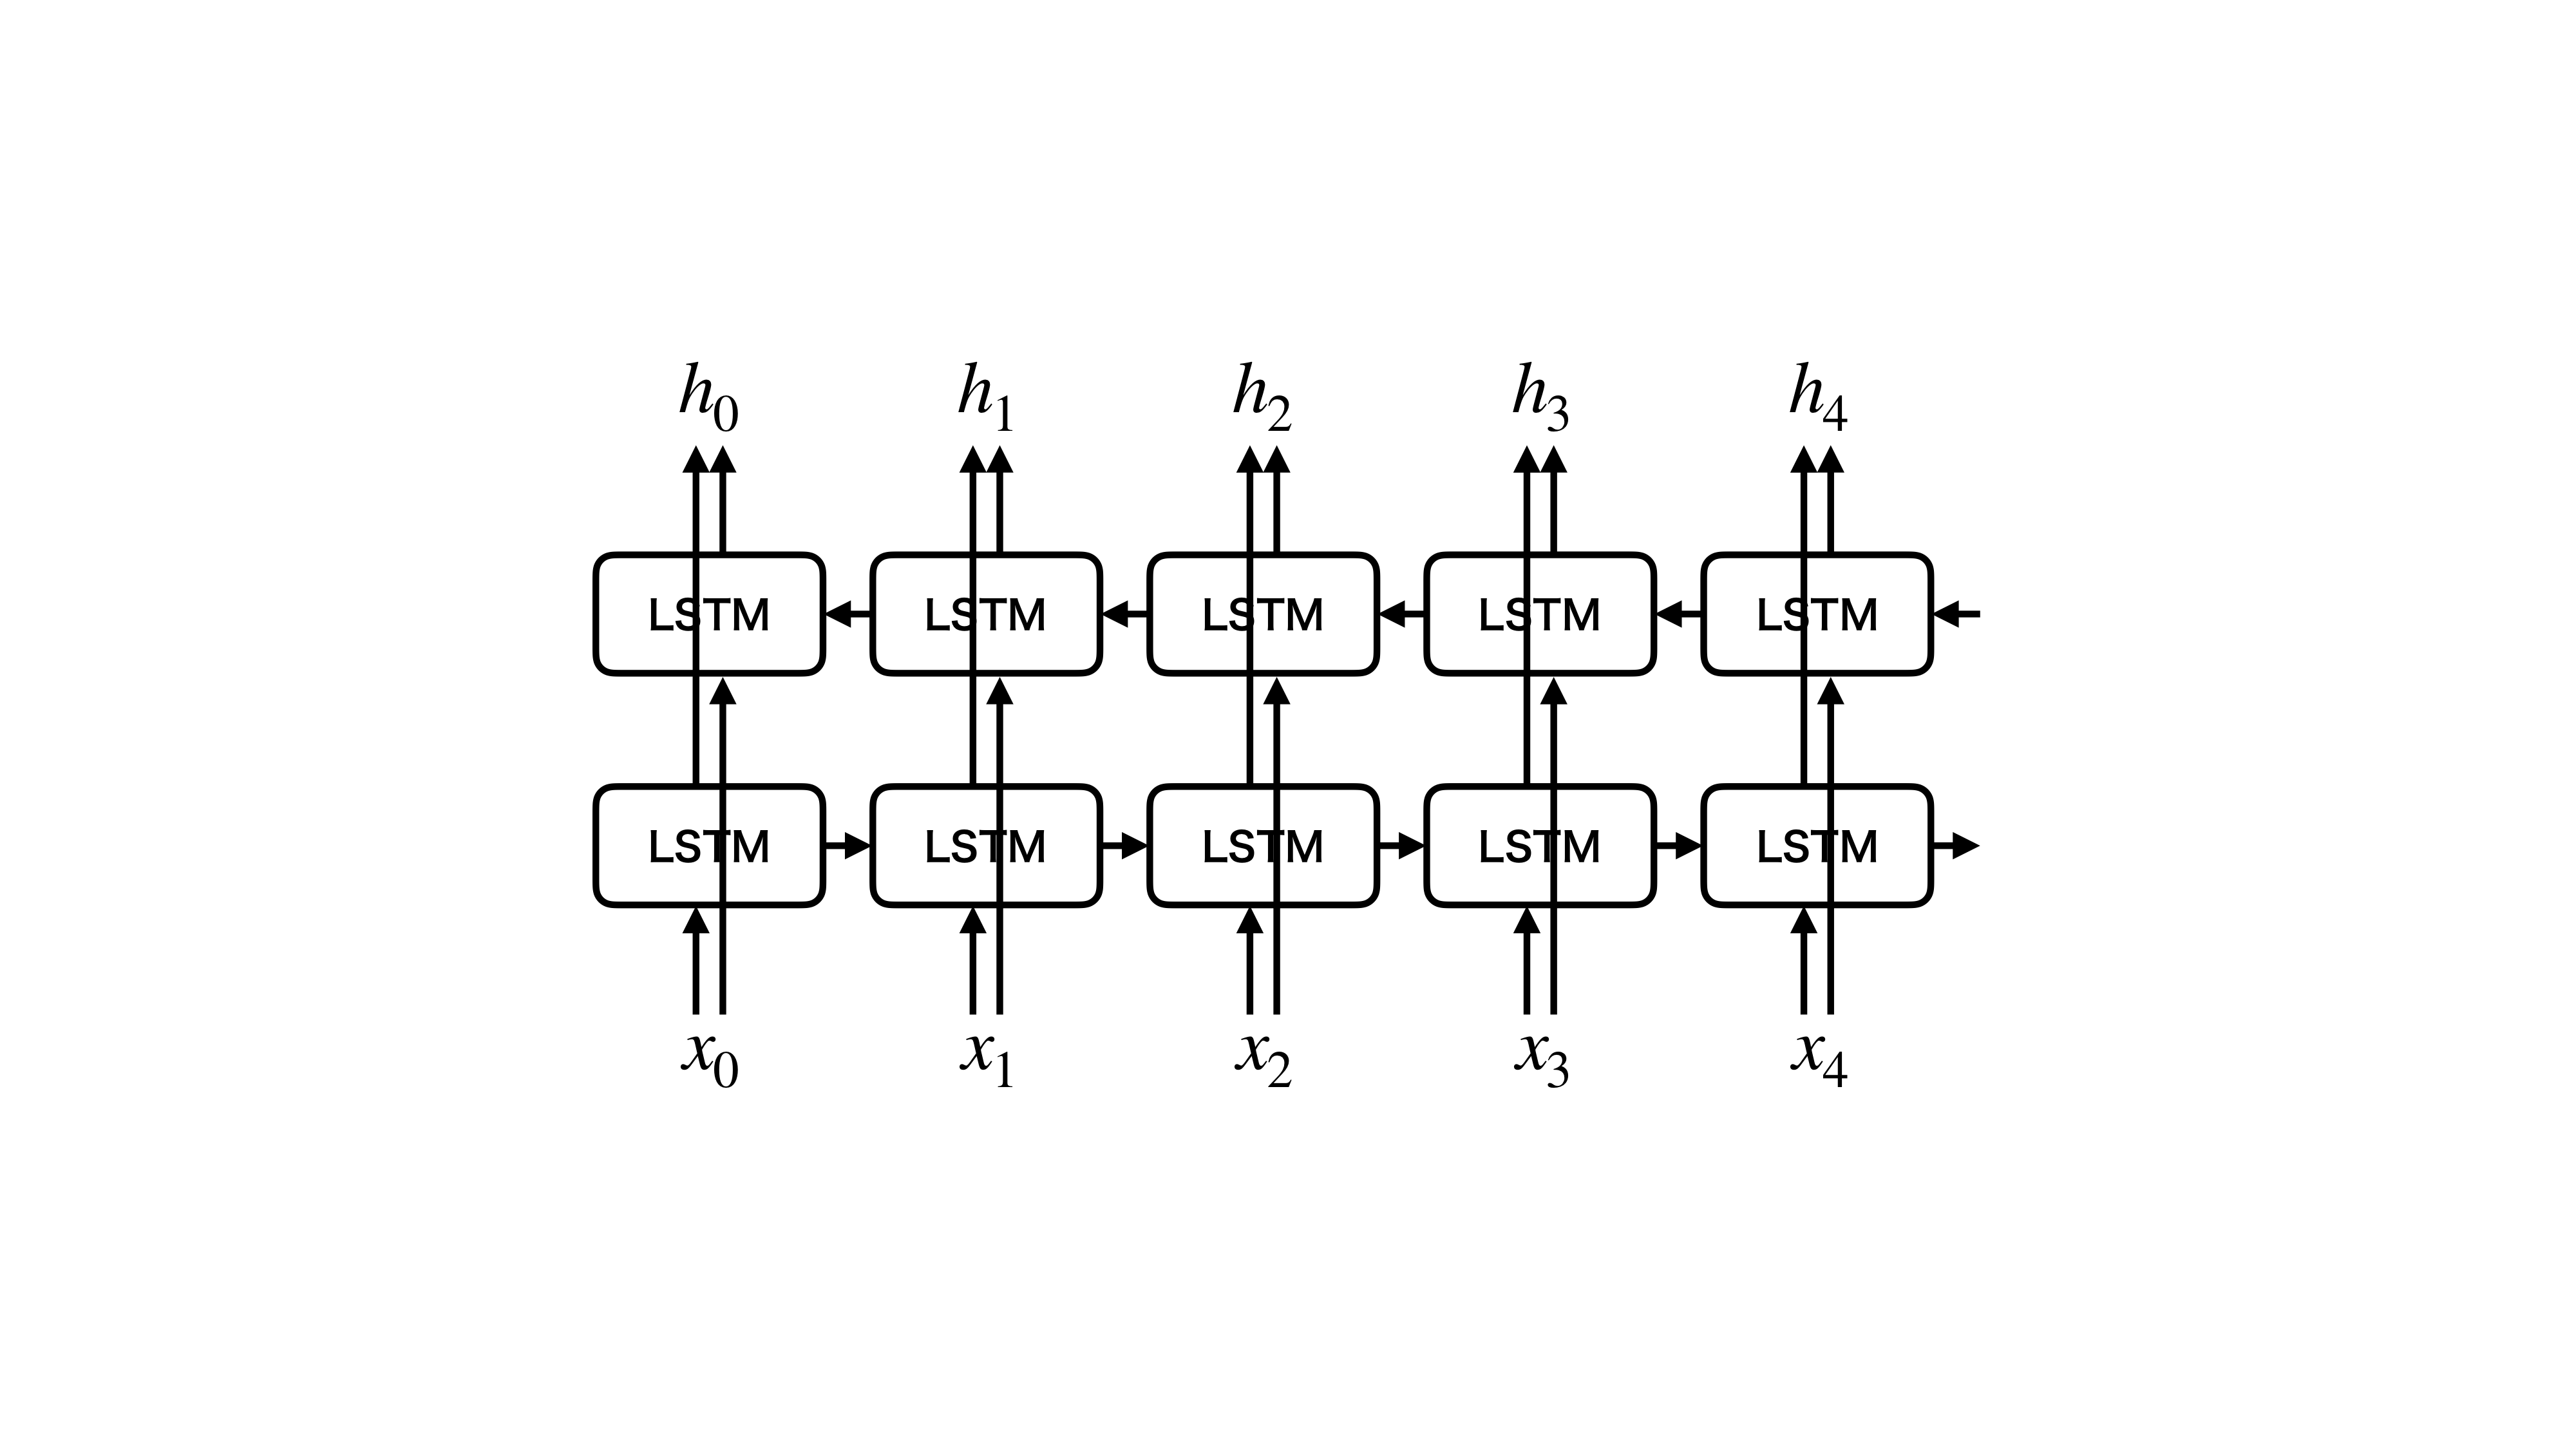
\includegraphics[trim = 0 200 0 200, width=1.0\textwidth, clip]{Figure/2DeepLearning/17BidirectionalLSTM.png}
 \caption[双方向LSTM]{双方向LSTM。Stacked LSTMとは異なり, 一段目のLSTMの出力は二段目の入力に使用されておらず, 計算はそれぞれ並列的に行われる。よって出力はLSTM二つ分の大きさになっている。}
 \label{17BidirectionalLSTM}
\end{figure}

リカレントニューラルネットワークはその構造が再帰的であるという点 (並列化が困難である) から, 学習が遅く, 重いという課題を抱えている。
また, 後述するエンコーダー・デコーダーモデルにおいては, データの系列の長さに応じた情報を確保できないという欠点が存在している。
\footnote{例えば, 機械翻訳を用いて$100$単語分の英文を日本語に翻訳する場合と$10$単語分の英文を翻訳する場合において, $100$単語分の英文が持つ情報の方が$10$単語分の英文と比べて多いことは明らかであるが, リカレントニューラルネットワークはこれらの情報の多さの違いに対応できず, 常に同じ量の情報から日本語を生成してしまう。}
次節では, このような問題を解決するための注意機構 (Attention) という技術を解説する。


%%%%%%%%%%%%%%%%%%%%%%%%%%%%%%%%%%%%%%%%%%%%%%%%%%%%%%%%%%%%%%%%%%%%%%%%%%%%%%%%%%%%%%%%%%%%%%%%%%%%%
\section{Attention} \label{DL:Attention}

Attention\cite{BahdanauAttention, LuongAttention}とはエンコーダー・デコーダーモデルに使用され, デコーダー部のある系列がエンコーダー部のどこに注意するかを計算する機構である。
主に機械翻訳や意味理解などに使用されており, 様々な応用が議論されているが, ここでは基本的なAttentionの理論と考え方についてのみ解説する。

\ref{DL:Atten:EncoderDecoderModel}項では, まずAttentionを理解する上で必要不可欠なエンコーダー・デコーダーモデルについて述べ, その中で前節のリカレントニューラルネットワークが抱える問題について紹介する。
次に, \ref{DL:Atten:Attention}項でAttentionの理論や計算について述べる。


%%%%%%%%%%%%%%%%%%%%%%%%%%%%%%%%%%%%%%%%%%%%%%%%%%%%%%%%%%%%%%%%%%%%%%%%
\subsection{エンコーダー・デコーダーモデル} \label{DL:Atten:EncoderDecoderModel}

LSTMを用いたエンコーダー・デコーダーモデルの大まかな構成を図\ref{18EncoderDecoderLSTM}に示す。
LSTMではエンコーダー部とデコーダー部を繋ぐ情報はエンコーダーの最後の層の出力を使用することが多い。
この場合, エンコーダー部は図\ref{9RNNOutputs}のMany to One, デコーダー部はOne to Manyを使用しており, エンコーダーによって抽出された情報はこのOneの部分に集められることになる。
この出力はMany to Oneの内, Manyであるデータの系列の長さ (系列長) に依存せず, 常に同じ大きさとなる。
これは長い系列長であっても, 短い系列長であっても同じ量の情報を使用しているということを意味している。
したがって, より長い系列長や短い系列長を扱う場合は, そのデータが持つ情報を完全に保持, 表現することは難しく, 情報の欠損により性能が下がってしまうという問題があった。
例えば, 機械翻訳において英文の和訳を考えると, エンコーダー部は英文を受け取り, デコーダー部は日本語の文章を出力する。
この時, 長い英文の翻訳にはより長い日本語の文章が必要な事は明らかであるが, LSTMのみを用いたエンコーダー・デコーダーモデルではこの文の長さの違いに対応する事ができない。

\begin{figure}[htbp]
 \centering
 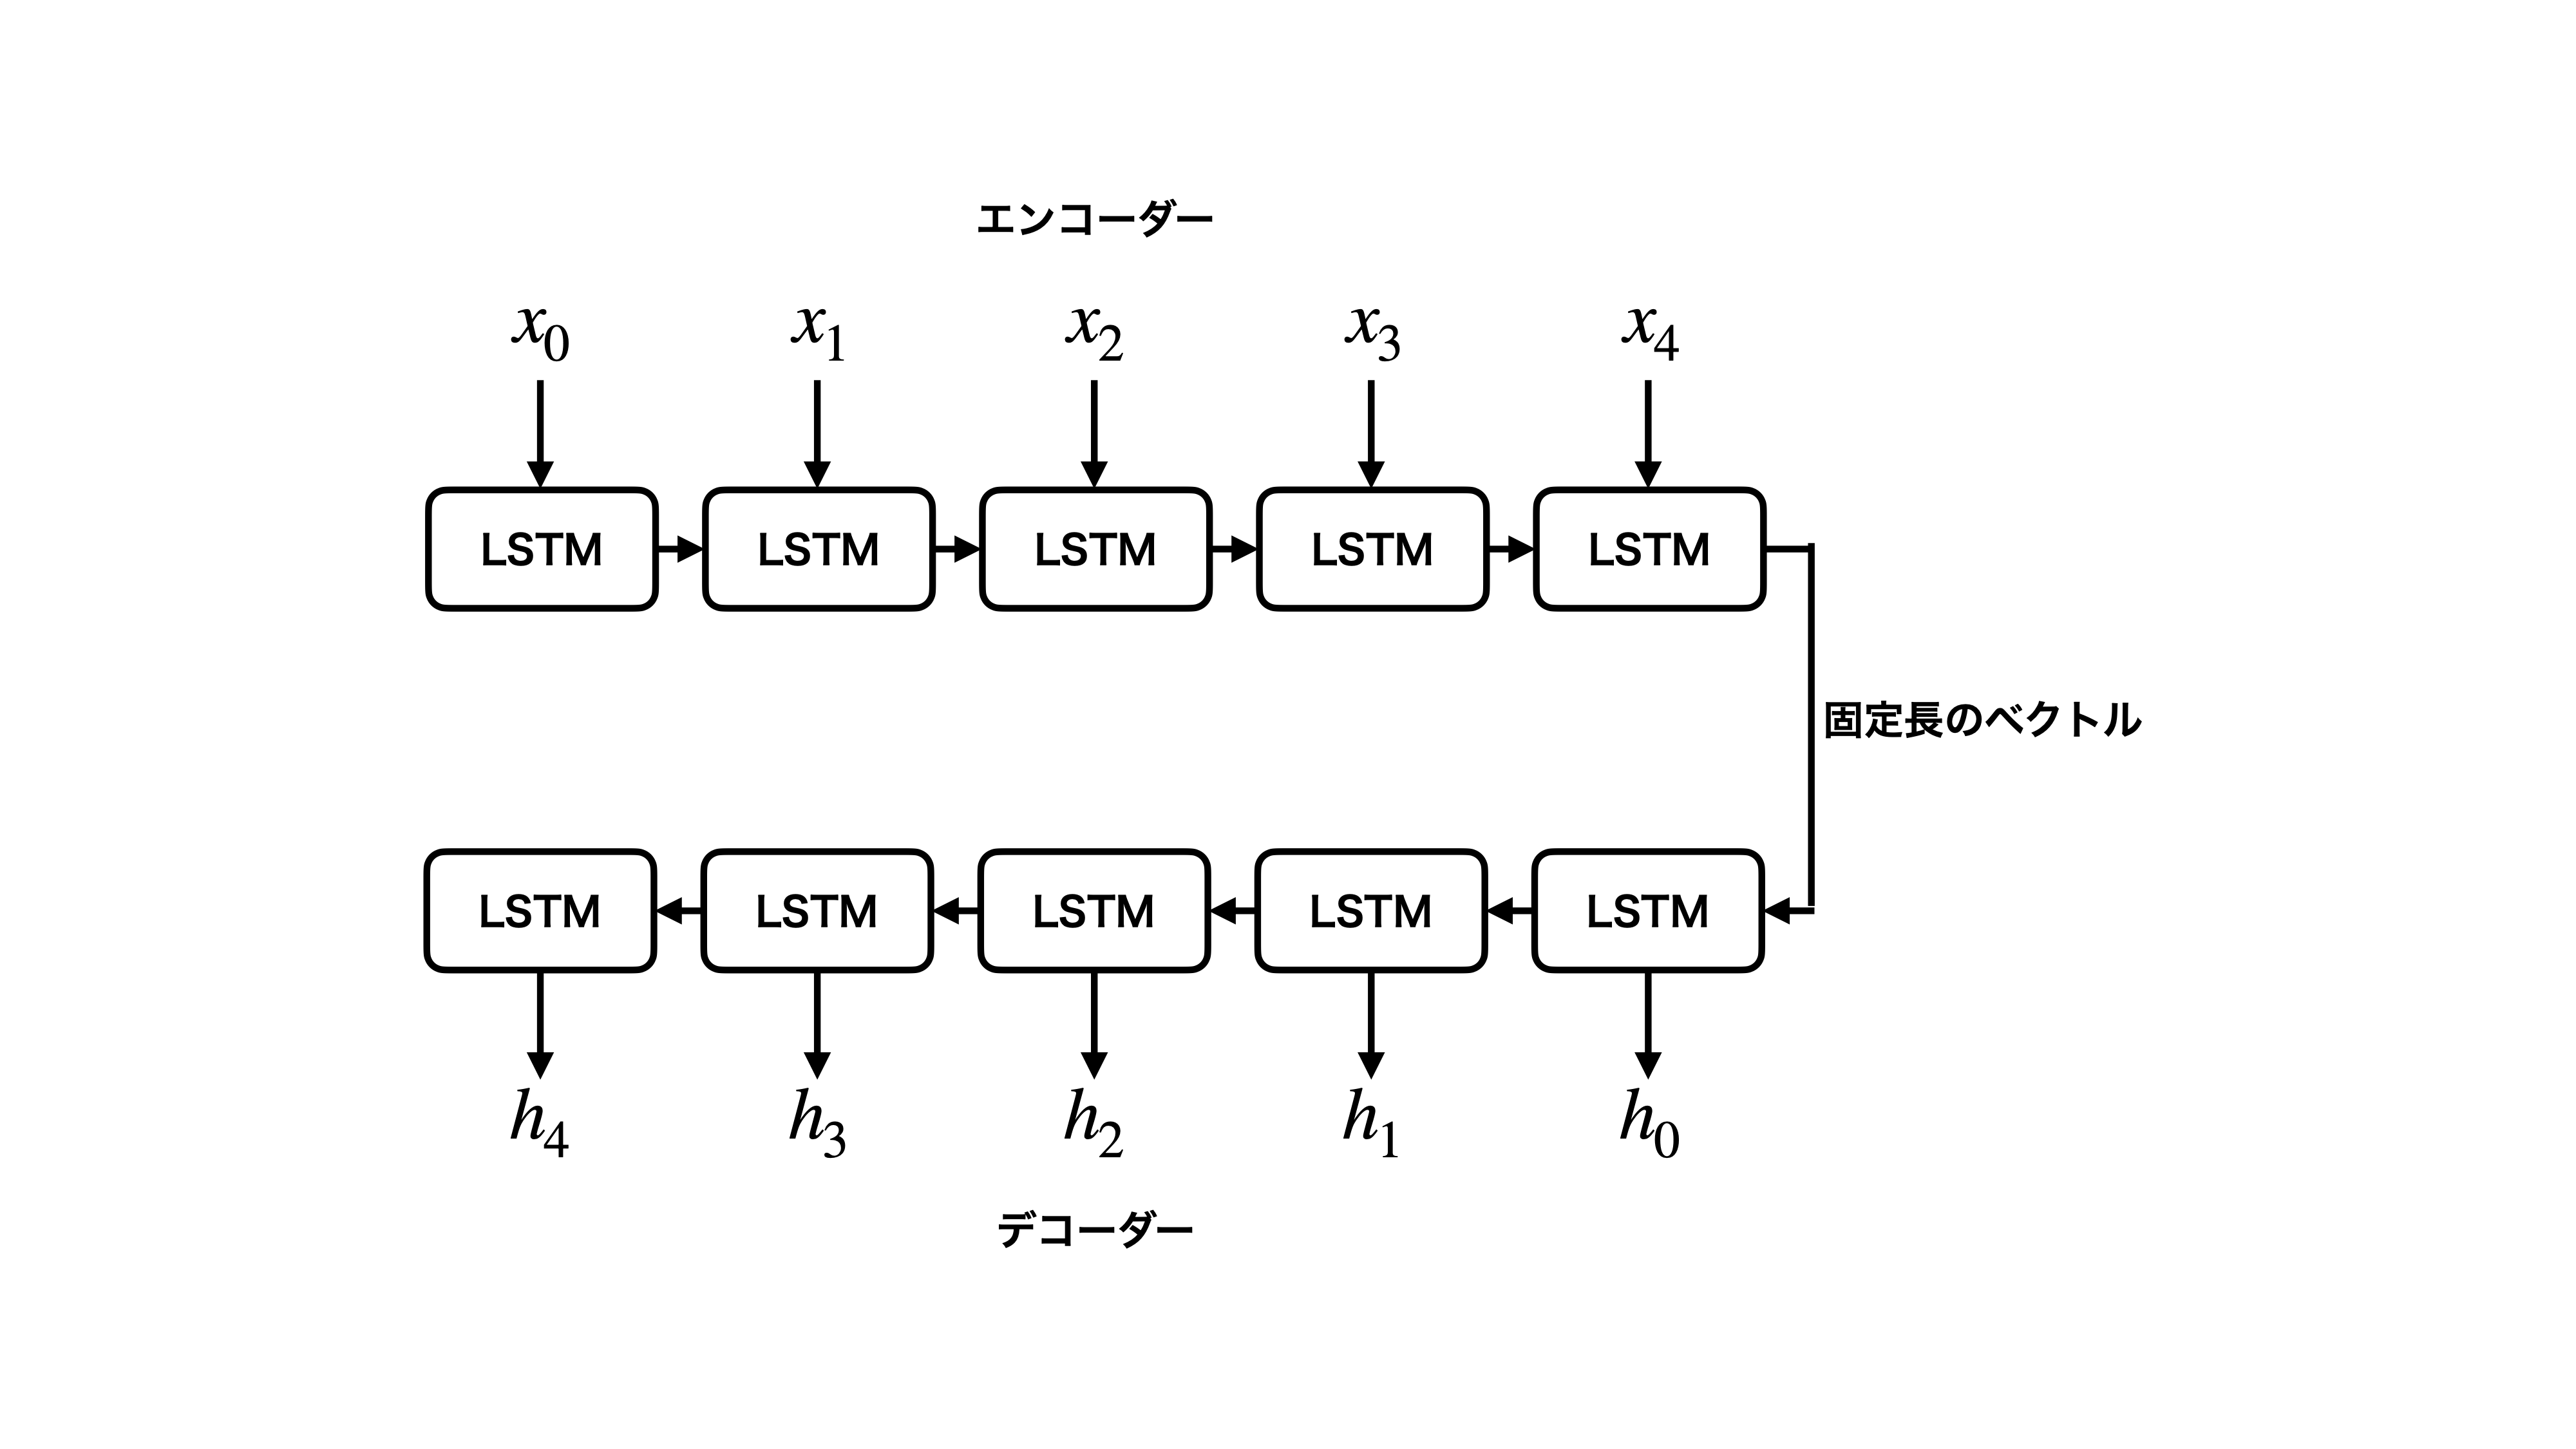
\includegraphics[trim = 100 100 100 200, width=1.0\textwidth, clip]{Figure/2DeepLearning/18EncoderDecoderLSTM.png}
 \caption[LSTMによるエンコーダー・デコーダーモデル]{LSTMによるエンコーダー・デコーダーモデル。図上部がエンコーダー部, 図下部がデコーダー部である。エンコーダー部の入力${\mbox{\boldmath{$x$}}}$から抽出された情報は図右の固定長のベクトルへと集約される。デコーダー部ではこの固定長のベクトルを初期状態にして出力${\mbox{\boldmath{$h$}}}$の生成を行う。}
 \label{18EncoderDecoderLSTM}
\end{figure}

この問題を解決するための技術がAttentionである。
Attentionを組み込んだLSTMのエンコーダー・デコーダーモデルを図\ref{19EncoderDecoderAttention}に示す。
Attentionを用いないエンコーダー・デコーダーモデルとの大きな違いは, エンコーダー部がMany to OneからMany to Manyの構造に変更されている点である。
このようにエンコーダー部の構造を変える事によって, エンコーダー部は系列長 (Many) に依存した情報量を確保することができる。

Attentionを用いたエンコーダー・デコーダーモデルではデコーダー部の構造にも変更が加えられている。
具体的には, デコーダー部はデコーダー部の``ある"系列がエンコーダー部の``どの"系列に注目するかを計算する事によって, エンコーダー部から必要な情報を抽出している。
どの系列に注意するかについての度合いをAttention Weightといい, Attention Weightはエンコーダー部の全ての系列についての重みである為, 実際にはエンコーダー部の系列長だけ次元を持ったベクトルである。\footnote{Attention Weightはデコーダーの個々の系列について個別に計算される。}
現在, Attention Weightを計算する方法が幾つか存在し, 代表的な計算方法について次項で述べる。

\begin{figure}[htbp]
 \centering
 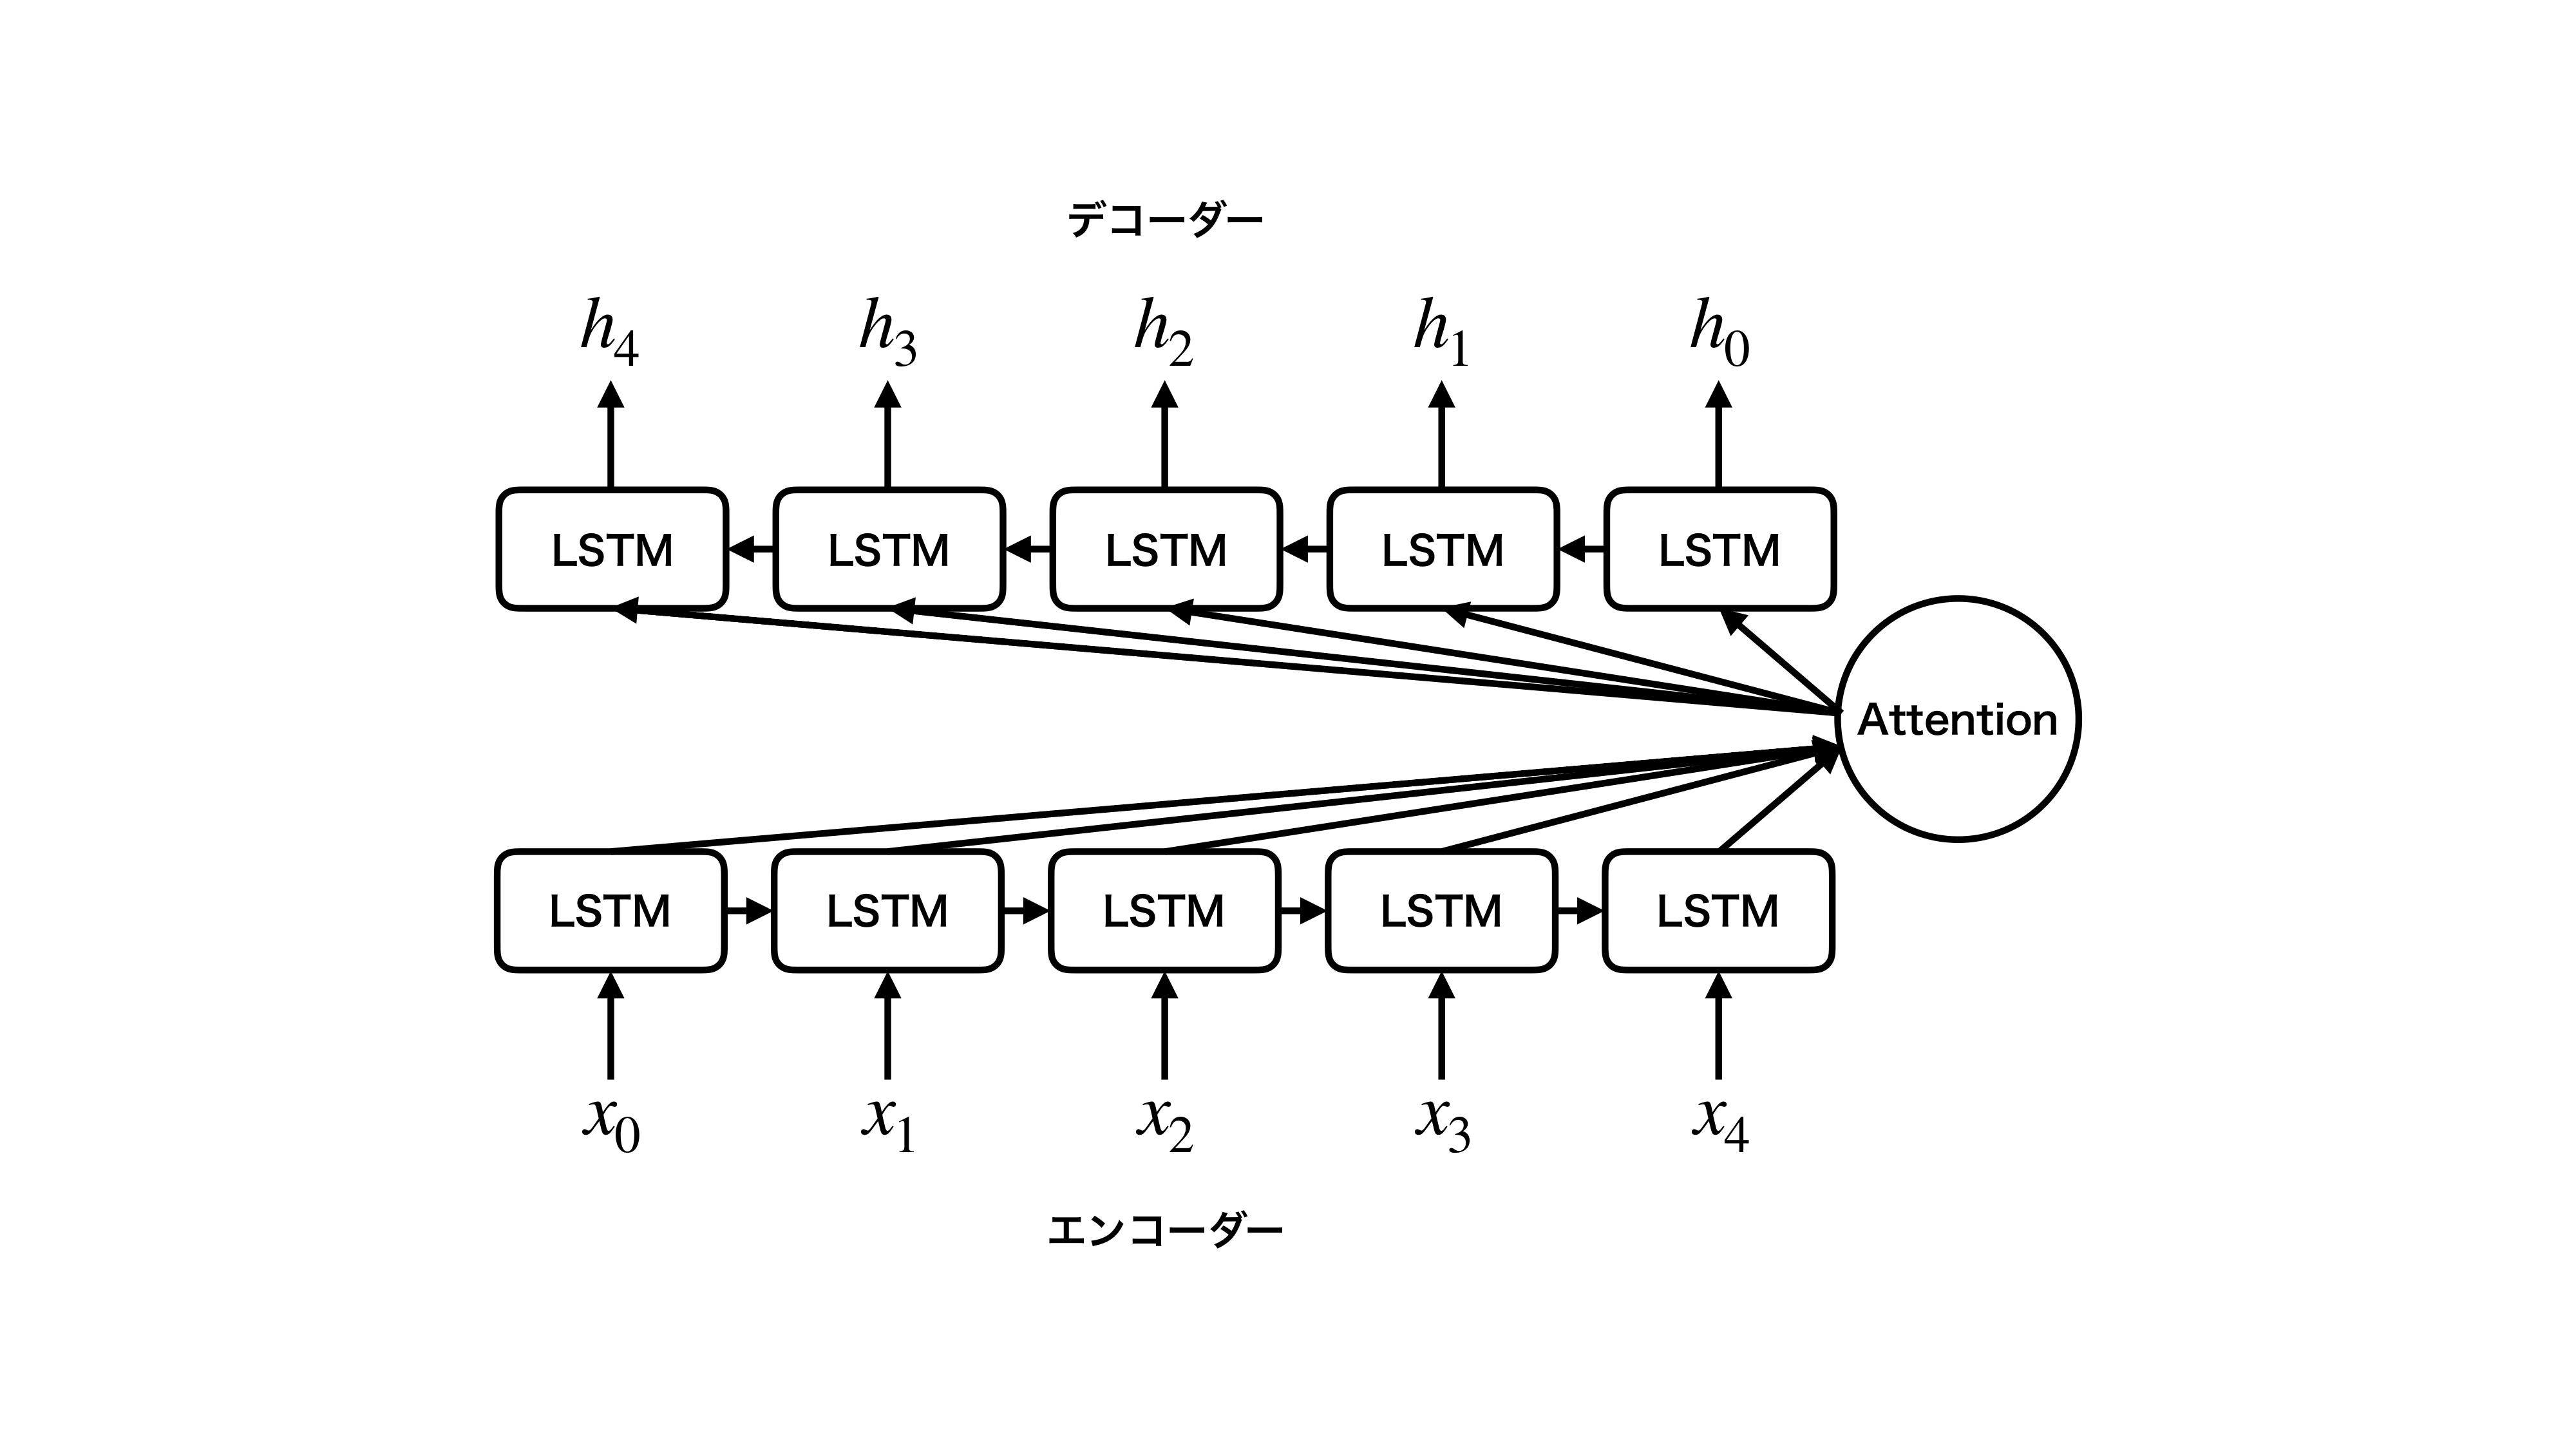
\includegraphics[trim = 100 0 100 0, width=1.0\textwidth, clip]{Figure/2DeepLearning/19EncoderDecoderAttention.png}
 \caption[AttentionとLSTMによるエンコーダー・デコーダーモデル]{AttentionとLSTMによるエンコーダー・デコーダーモデル。図上部がエンコーダー部, 図下部がデコーダー部である。エンコーダー部はMany to Manyの出力になっており, デコーダー部はデコーダー部の``ある"系列がエンコーダー部の``どの"系列に注目するかを計算する事によって, エンコーダー部から必要な情報を抽出している。}
 \label{19EncoderDecoderAttention}
\end{figure}


%%%%%%%%%%%%%%%%%%%%%%%%%%%%%%%%%%%%%%%%%%%%%%%%%%%%%%%%%%%%%%%%%%%%%%%%
\subsection{Attention} \label{DL:Atten:Attention}

\begin{figure}[htbp]
 \centering
 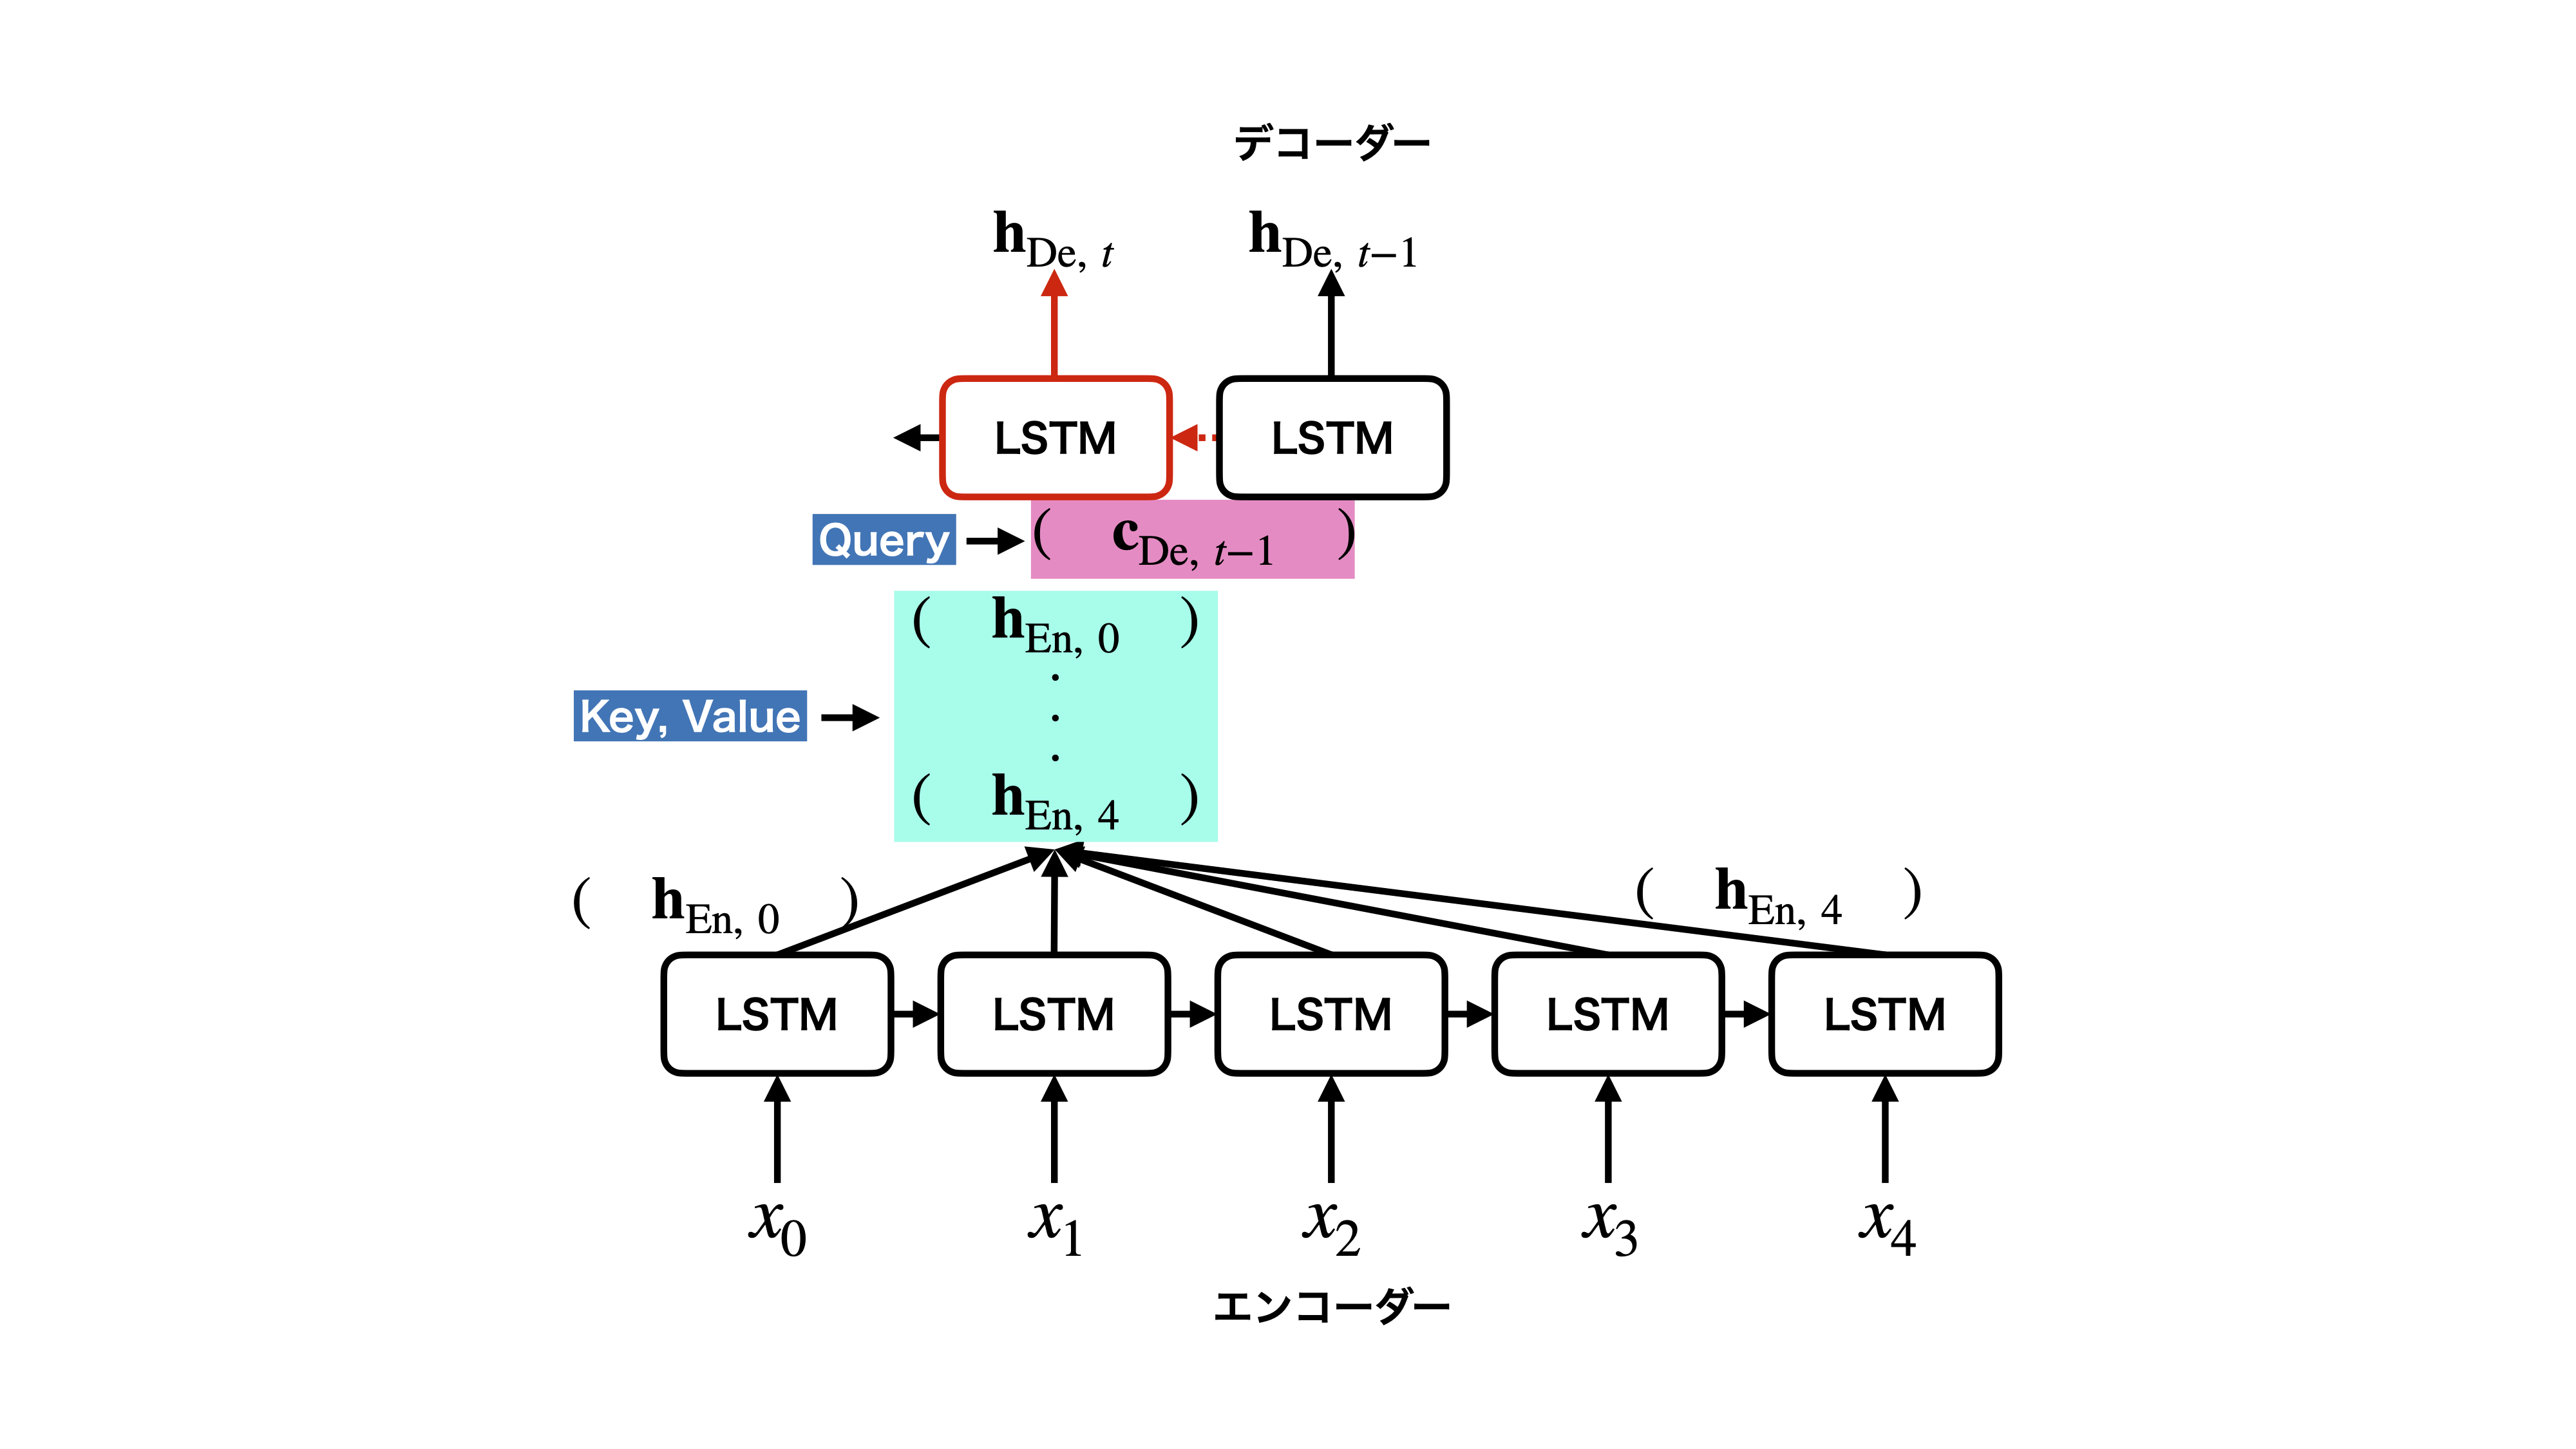
\includegraphics[trim = 100 0 100 0, width=1.0\textwidth, clip]{Figure/2DeepLearning/19KeyValueQuery.png}
 \caption{Key, Value, Queryの図示}
 \label{19KeyValueQuery}
\end{figure}

Attentionでは一般にエンコーダー部の出力の事をKey, Valueという。
また, デコーダー部のある系列$t$についてAttention Weightを計算する際, 直前の系列$t-1$のデコーダーの隠れ状態 (${\mbox{\boldmath{$c$}}}_{{\rm De},\ t-1}$) をQueryという (図\ref{19KeyValueQuery})。
ここでAttention Weightとはデコーダー部の個々の系列について個別に計算される量である為, Queryについても同様にデコーダー部の系列の数だけ存在する事に注意する。
一方KeyやValueはデコーダー部の全ての系列について共通である。
本項では, デコーダー部のある系列$t$についてのAttentionに関する量を「$t$番目の」と呼ぶこととすると, デコーダーの隠れ状態 (${\mbox{\boldmath{$c$}}}_{{\rm De},\ t-1}$) は$t$番目のQueryとなり, この$t$番目のQueryによって計算されるAttention Weightは$t$番目のAttention Weightとなる。

一般に, Key, Valueについて$t$番目のQueryを用いて, $t$番目のAttention Weightを計算する方法として, Additive Attention\cite{BahdanauAttention}, Dot-Product Attention\cite{LuongAttention}のどちらかの手法を用いることが多い。\footnote{どちらの手法も本質的な意味合いは同じであり, 後述する処理の違いなどの差しかない。}
それぞれの計算を図\ref{20Attention}に示す。
どちらの手法においても$t$番目のAttention Weightは$t$番目のエネルギーをソフトマックス関数によって規格化したものとなっている。\footnote{このエネルギーとは物理学のエネルギーとは全く異なるものであるが, ここでは原著論文に従ってエネルギーと呼ぶこととする。}
$t$番目のエネルギーを計算する手法はそれぞれ異なり, Additive Attentionでは学習可能な重みを用いた全結合層によって値を抽出し, Dot-Product Attentionでは単にKeyとQueryを掛け合わせることで計算している。
この為, Additive AttentionではAttentionの内部で重みの更新・学習が発生し, Dot-Product Attentionと比較して動作が遅くなるという欠点が存在する。
一方, Dot-Product AttentionはKeyとQueryを直接掛け合わせる為, 行列演算の制約からKeyとQueryのそれぞれの大きさについて制限がある。
ここで, エンコーダー部の系列長を$\rm M$とすると$t$番目のAttention Weightの大きさが$\rm M$次元のベクトルとなっていることがわかる。
Attentionでは得られた$t$番目のAttention WeightとValueを用いてデコーダー部の為の情報 ($t$番目のコンテキスト) が計算される。
$t$番目のコンテキストをどの様にデコーダー部に使用するかに関しては\ref{Net:VLSTM:StructureofVLSTM}項で述べる。\\

\begin{figure}[htbp]
 \centering
 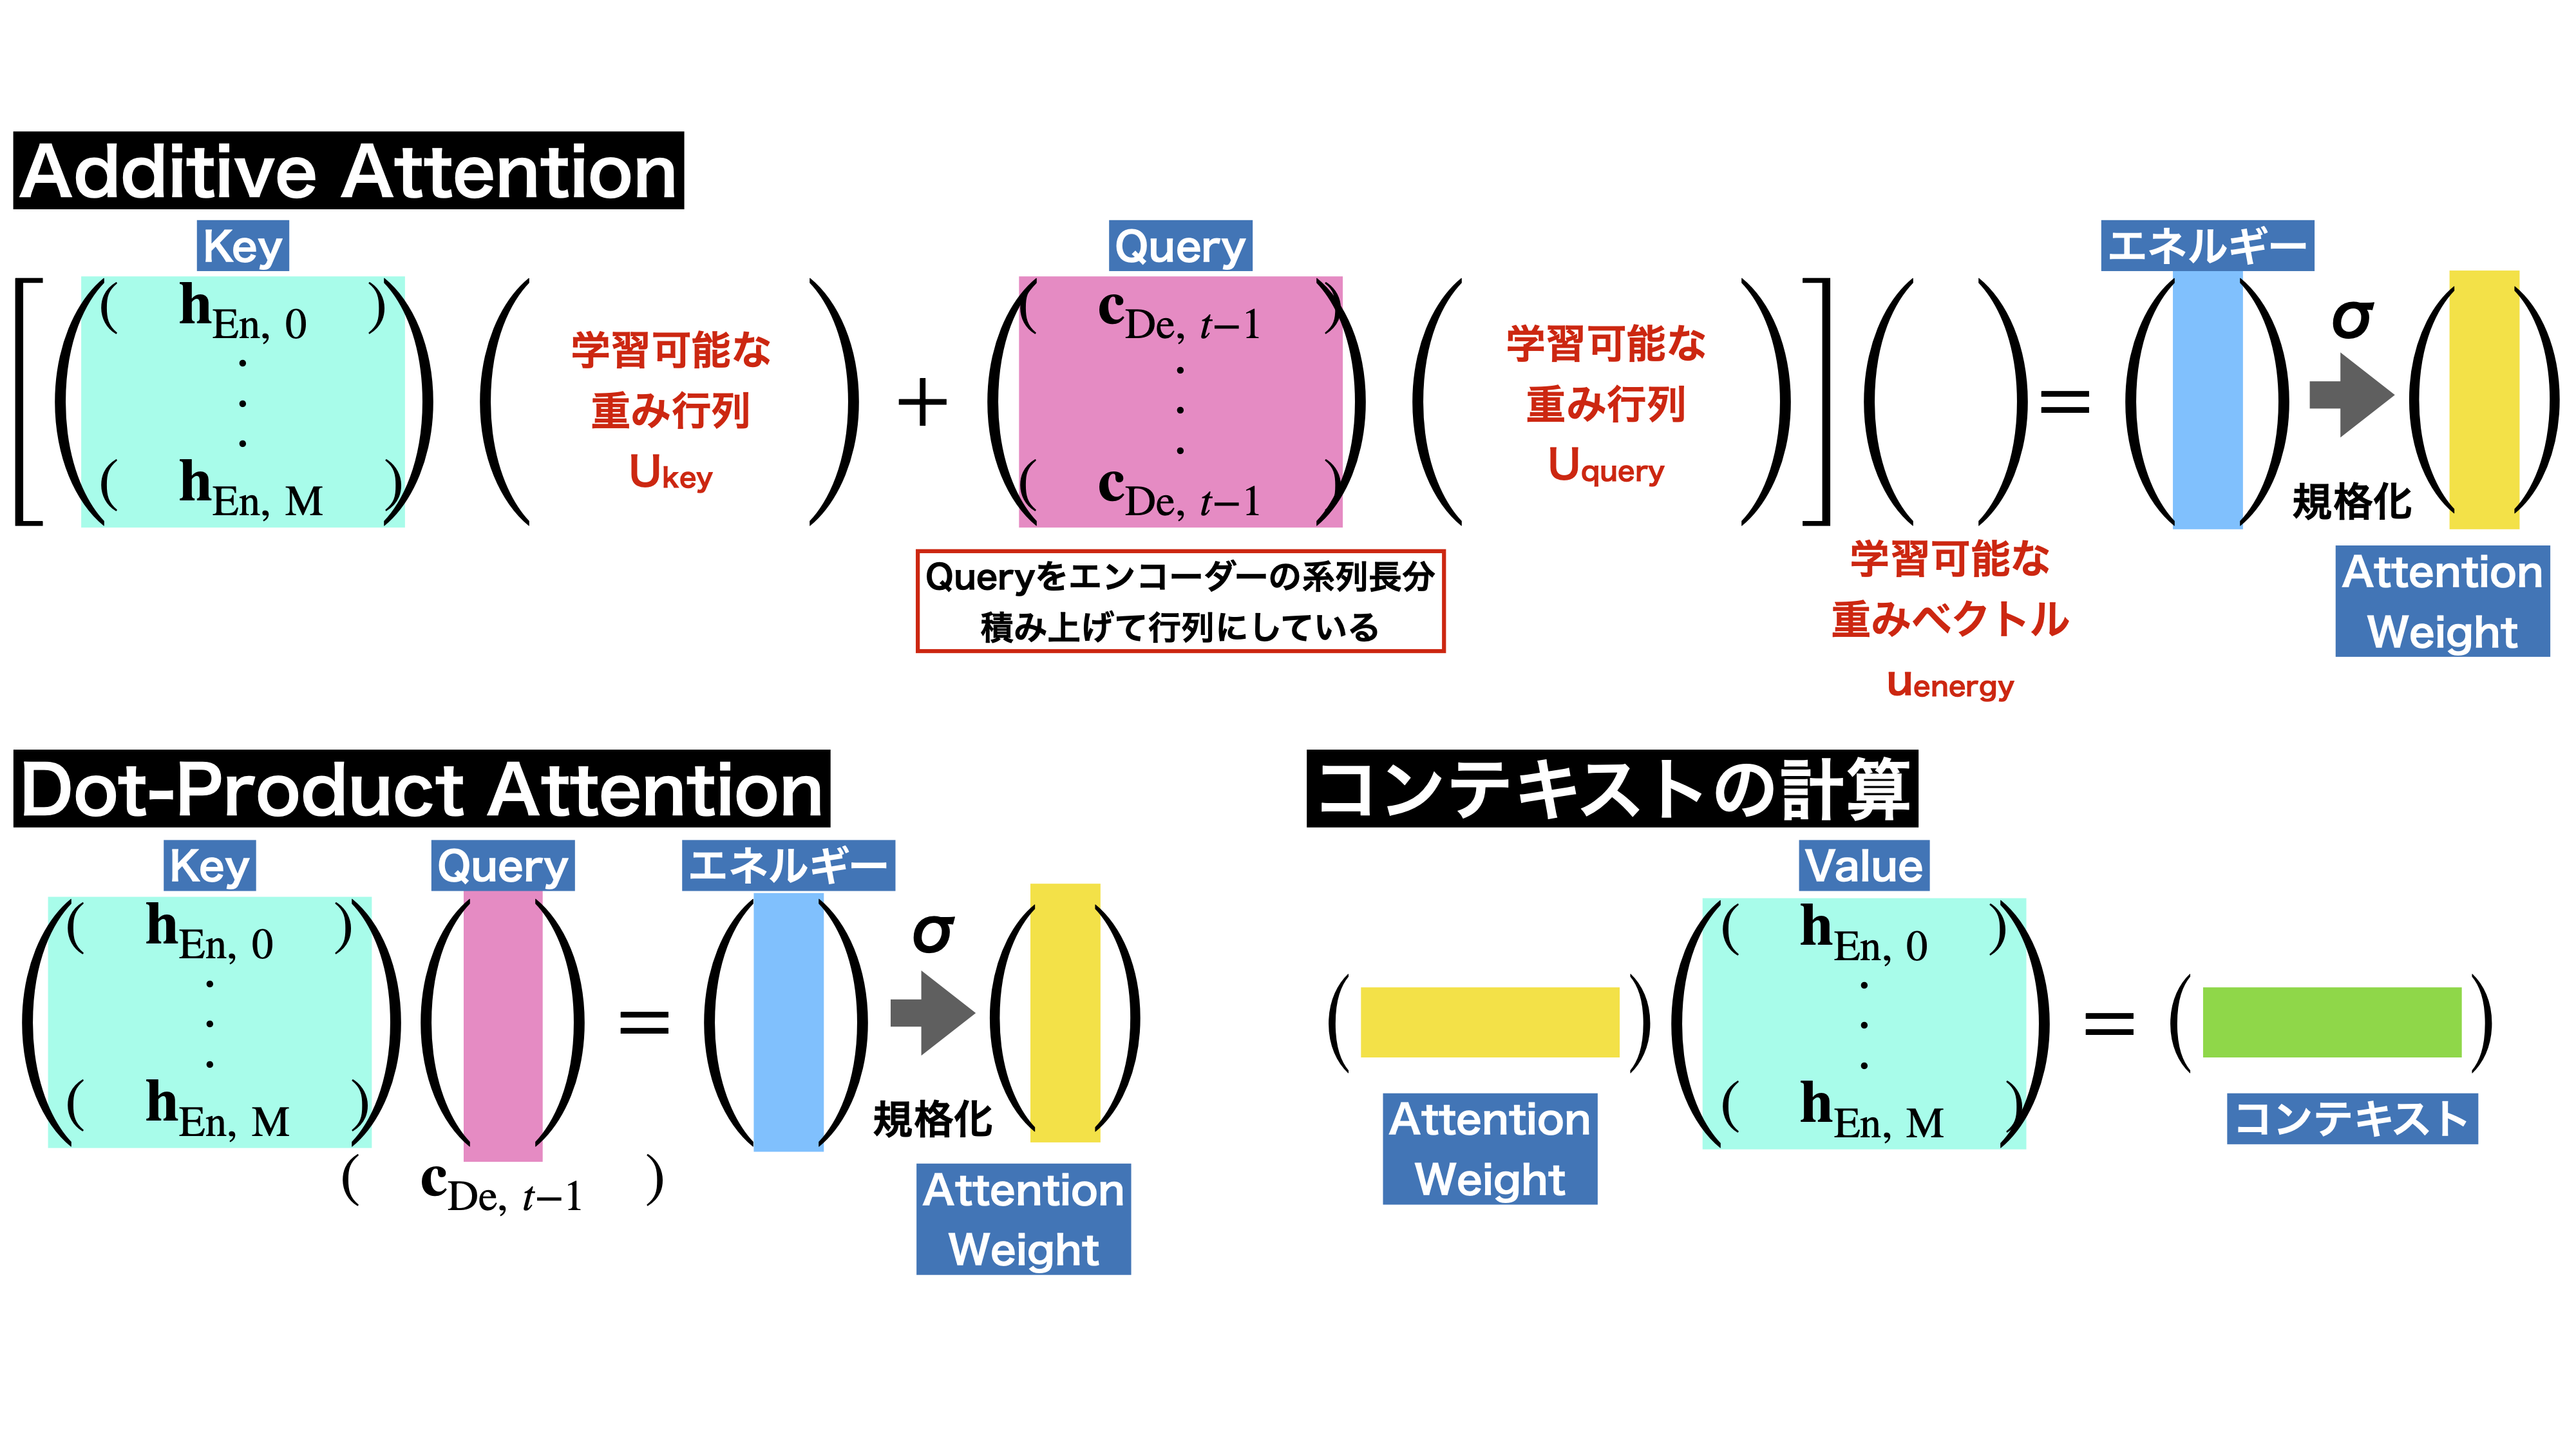
\includegraphics[trim = 0 100 0 100, width=1.0\textwidth, clip]{Figure/2DeepLearning/20Attention.png}
 \caption{Additive Attention と Dot-Product Attention}
 \label{20Attention}
\end{figure}

AttentionはAttention Weightを確認する事によってネットワーク内部の理解につながるという点でも非常に強力である。
本研究におけるAttention Weightに関する具体的な図は図\ref{3-4-3-3AttentionWeight}に示している。
Attention``Attention is all you need\cite{AttentionIsAllYouNeed}''と言われるほど, 近年非常に注目されている技術である。
ここでは, AttentionをLSTMの補助として使用している例を挙げたが, Attentionは様々な技術と組み合わせられる。
またそれだけでなく, Attentionのみを用いて構成された, Transformerと呼ばれるモデルは2021年現在において, 自然言語処理の標準的なネットワークであると言われるほどの性能と, LSTMでは実現できなかった速さを両立している。


%%%%%%%%%%%%%%%%%%%%%%%%%%%%%%%%%%%%%%%%%%%%%%%%%%%%%%%%%%%%%%%%%%%%%%%%%%%%%%%%%%%%%%%%%%%%%%%%%%%%%
\section{ハイパーパラメータ} \label{DL:HyperParameter}

ここまでで述べたように深層学習は教師あり学習であるため, 訓練データを用いて重みの更新を行い, ネットワークの重みを最適化していく。
しかし, ネットワークはネットワーク自体を構築するための, 学習によって更新されないパラメータをいくつか持っている。
このようなパラメータをハイパーパラメータという。
ハイパーパラメータは学習前に設定しておく必要があり, ネットワークの性能を引き出すためには適切な最適化 (ハイパーパラメータ・チューニング) が必要がある。
ハイパーパラメータの種類や数はネットワークの構造によって大きく異なるが, 一般にチューニングが必要とされるハイパーパラメータについて以下に示す。

\begin{itemize}
  \item 最適化手法 (Optimizer) : RMSPropやAdamといった重み更新の為の最適化手法
  \item 学習率 (Learning rate) : 重み更新のステップ幅
  \item エポック数 (Epochs) : 学習回数・訓練データを一周学習することを1エポックという
  \item バッチサイズ (Batch size) : ミニバッチ学習における訓練データサンプルの大きさ
  \item ノード数 (Node) : 重み行列の大きさ
  \item 層の数 (Layer) : フィードフォワードネットワークにおける全結合層の数
\end{itemize}

これらはハイパーパラメータの一例であり, それぞれについて適切に選ぶ必要がある。
ハイパーパラメータの探索手法も幾つか提案されており, ランダムサーチやグリッドサーチ, ベイズ最適化などが用いられている。

以上が本論文のための深層学習の導入である。
この\ref{chap:DeepLearning}章を前提として, \ref{chap:Networks}章での本研究で使用したネットワークの構造を解説していく。
以降の章では, ここで挙げた深層学習の用語を説明せずに使用するが, その場合は適宜, 本章を参照していただきたい。
また, 本章の初めや\ref{DL:NeuralNetwork}でも述べたように, 深層学習の実装に関しては様々なフレームワークがあるため, ここでの記載は省かせていただく, 本研究の実装に関しては付録\ref{sec:Code}や私のGitHub\cite{GitHubGotoK}にまとめている。
















% !TEX root = ../MasterThesis_goto_v1.tex

%%%%%%%%%%%%%%%%%%%%%%%%%%%%%%%%%%%%%%%%%%%%%%%%%%%%%%%%%%%%%%%%%%%%%%%%%%%%%%%%%%%%%%%%%%%%%%%%%%%%%
\chapter{崩壊点検出の為のネットワーク} \label{chap:Networks}

本章では, 深層学習を用いた崩壊点検出のために構築したネットワークの詳細について述べる。

まず\ref{Net:Data}節では, 本研究で取り扱うデータの特性について述べる。
前述したように本研究で使用するデータは全てMCシミュレーションデータである。
\ref{Net:Data}節ではそのようなシミュレーションデータに関してソフトウェアの性質や物理的な性質について解説する。
ただし, ネットワークの学習に使用した訓練データについては個々のネットワークの解説で適宜述べる。

次に, \ref{Net:forVertexFinderwithDL}節では, 深層学習を使用して, どのように崩壊点検出を実現するかについて, 発想と構築したネットワークの役割について概説する。
また, 使用したハードウェアやソフトウェア・フレームワークの環境などについてもここで述べる。

\ref{Net:PairModel}節と\ref{Net:VertexLSTM}節では, 本研究のために構築した個々のネットワークについて, 構造・学習・性能と評価について議論する。


%%%%%%%%%%%%%%%%%%%%%%%%%%%%%%%%%%%%%%%%%%%%%%%%%%%%%%%%%%%%%%%%%%%%%%%%%%%%%%%%%%%%%%%%%%%%%%%%%%%%%
\section{データ} \label{Net:Data}

本研究で使用したシミュレーションデータについて\ref{Net:Data:DataProperty}項では, データ全体についてのソフトウェアや物理的性質に関して述べる。
\ref{Net:Data:TrackInformationandPreprocessing}項では, 本研究で使用する飛跡についての情報と深層学習に使用するための前処理について紹介する。


%%%%%%%%%%%%%%%%%%%%%%%%%%%%%%%%%%%%%%%%%%%%%%%%%%%%%%%%%%%%%%%%%%%%%%%%
\subsection{データ全体の性質} \label{Net:Data:DataProperty}

本研究ではシミュレーションデータとして, イベントジェネレーター WHIZARD\cite{WHIZARDpaper}を用いて生成されたILDフルディテクターシミュレーションデータを使用した。
これらのデータは後述するLCFIPlusでの性能評価\cite{LCFIPlusPaper}で使用されたデータと同一のものである。
MCシミュレーションデータの性質を表\ref{MCSimulationDataProperty}に示す。

\begin{table}[htb]
 \centering
 \small
  \begin{tabular*}{0.75\textwidth}{@{\extracolsep{\fill}}l l}\hline
    イベントジェネレーター & WHIZARD\\
    検出器 & ILDフルディテクターシミュレーション\\
    重心系エネルギー & Z粒子の質量 ($91.2\ \mathrm{GeV}$)\\ 
    終状態 & $\rm e^+ e^- \to b\bar{b},\  c\bar{c},\  q\bar{q}$\\ 
    Beamstrahlung/ISR & なし\\
    ビーム偏極 & なし\\\hline
  \end{tabular*}
  \caption{MCシミュレーションデータの性質}
  \label{MCSimulationDataProperty}
\end{table}

ここで, 終状態の$\rm b$はボトム・フレーバー, $\rm c$はチャーム・フレーバー, $\rm q$はアップ, ダウン, ストレンジ・フレーバーのクォークをそれぞれ表している。
これらのクォーク対は自然界で直ちにハドロンを形成し, 特にボトム, チャーム・フレーバーの場合は再構成可能なSecondary Vertexを残すジェットとなる。

データについて, 終状態$\rm b\bar{b}$のデータは$15$個のサンプルに, 終状態$\rm c\bar{c}$のデータは$13$個のサンプルに分け使用した。
終状態$\rm b\bar{b}$のデータは$12$個のサンプルに分離したが, 深層学習ネットワークの学習には使用していない。
深層学習を含めた教師あり学習では, 健全性のため学習に使用する訓練データと学習時の性能観測に使用する検証データ, 最終的な評価に使用するテストデータは分けなければならない。
したがって個々のサンプル毎に用途を明らかにし, 訓練データの作成とネットワークの評価に使用するデータの詳細について, サンプルに含まれる事象数や飛跡数, 用途を表\ref{DataSamples}にまとめる。

\begin{table}[htbp]
 \centering
 \small
  \begin{tabular*}{1.0\textwidth}{@{\extracolsep{\fill}}c c c l}\hline
     データ名 & 事象数 & 飛跡数 & 用途\\ \hline \hline
    $\rm c\bar{c}-01$ & 69581 & 1344465 & データの調査/フレーバータギングの訓練データの作成\\ \hline
    $\rm c\bar{c}-02$ & 42204 & 814074 & 動作テスト/フレーバータギングの訓練データの作成\\ \hline
    $\rm c\bar{c}-03$ & 38662 & 748027 & 飛跡対についてのネットワークの訓練データの作成\\
    $\rm c\bar{c}-04$ & 38712 & 747625 & 飛跡対についてのネットワークの訓練データの作成\\ \hline
    $\rm c\bar{c}-05$ & 38655 & 748089 & 任意の数についてのネットワークの訓練データの作成\\\hline
    $\rm c\bar{c}-06$ & 38645 & 747548 & ネットワーク/崩壊点検出の評価\\
    $\rm c\bar{c}-07$ & 38643 & 747312 & ネットワーク/崩壊点検出の評価\\
    $\rm c\bar{c}-08$ & 38715 & 748801 & ネットワーク/崩壊点検出の評価\\ \hline 
    $\rm c\bar{c}-09$ & 38705 & 747725 & フレーバータギングの訓練データの作成\\ 
    $\rm c\bar{c}-10$ & 38721 & 748025 & フレーバータギングの訓練データの作成\\
    $\rm c\bar{c}-11$ & 38587 & 747819 & フレーバータギングの訓練データの作成\\ \hline
    $\rm c\bar{c}-12$ & 38723 & 748904 & LCFIPlusとの比較\\
    $\rm c\bar{c}-13$ & 35848 & 693780 & LCFIPlusとの比較\\ \hline\hline
    $\rm b\bar{b}-01$ & 62795 & 1326168 & データの調査/フレーバータギングの訓練データの作成\\ \hline
    $\rm b\bar{b}-02$ & 42950 & 909082 & 動作テスト/フレーバータギングの訓練データの作成\\
    $\rm b\bar{b}-03$ & 34985 & 738105 & 動作テスト/フレーバータギングの訓練データの作成\\ \hline
    $\rm b\bar{b}-04$ & 34952 & 739130 & 飛跡対についてのネットワークの訓練データの作成\\ 
    $\rm b\bar{b}-05$ & 35047 & 741568 & 飛跡対についてのネットワークの訓練データの作成\\ \hline
    $\rm b\bar{b}-06$ & 35008 & 740662 & 任意の数についてのネットワークの訓練データの作成\\ \hline
    $\rm b\bar{b}-07$ & 34000 & 718057 & ネットワーク/崩壊点検出の評価\\
    $\rm b\bar{b}-08$ & 33978 & 717972 & ネットワーク/崩壊点検出の評価\\ 
    $\rm b\bar{b}-09$ & 35008 & 740268 & ネットワーク/崩壊点検出の評価\\ \hline
    $\rm b\bar{b}-10$ & 34954 & 739320 & フレーバータギングの訓練データの作成\\ 
    $\rm b\bar{b}-11$ & 35012 & 740797 & フレーバータギングの訓練データの作成\\ 
    $\rm b\bar{b}-12$ & 34972 & 739953 & フレーバータギングの訓練データの作成\\ \hline
    $\rm b\bar{b}-13$ & 34986 & 739402 & LCFIPlusとの比較\\ 
    $\rm b\bar{b}-14$ & 34910 & 740933 & LCFIPlusとの比較\\ 
    $\rm b\bar{b}-15$ & 10243 & 216499 & LCFIPlusとの比較\\ \hline
  \end{tabular*}
  \caption{データサンプルの事象数と用途}
  \label{DataSamples}
\end{table}

後述する\ref{chap:Conparison}章の現行の手法であるLCFIPlusとの比較においてLCFIPlusのフレーバータギング (BDTs) の学習が必要である。
その為, BDTsの訓練データ作成に$\rm c\bar{c}-01,\ 02,\ 09,\ 10,\ 11,\ \rm b\bar{b}-01,\ 02,\ 03,\ 10,\ 11,\ 12$を用いた。
また, $\rm c\bar{c}-01,\ b\bar{b}-01$は本節のデータ特性の調査に使用し, $\rm c\bar{c}-02,\ b\bar{b}-02,\ 03$はネットワークの動作確認にも使用した。
ネットワークの訓練データの作成は$\rm c\bar{c}-03,\ 04,\ 05,\ b\bar{b}-04,\ 05,\ 06$を用いて行なった。
また, 訓練データの正解ラベルはMC情報やLCFIPlusのフィッターからの出力情報を使用した。\\

崩壊点検出を行うに当たって, 終状態による崩壊点の性質の違いに注意しなければならない。
終状態が$\rm c\bar{c}$の場合はチャーム・フレーバーのハドロンによるSecondary Vertexのみが生じる一方で, 終状態が$\rm b\bar{b}$の場合は$\rm b \to c$という崩壊過程を辿り, ボトム・フレーバーのハドロンによるSecondary Vertexと更にそこから派生したチャーム・フレーバーのハドロンによるTertiary Vertexが生じる。
それぞれのハドロン粒子の典型的な飛程は寿命$\tau$と光速$\tau$を用いて, ボトム・フレーバーの場合は$c \tau = 400-500 \ \mathrm{\mu m}$, チャーム・フレーバーの場合は$c \tau = 20-300 \ \mathrm{\mu m}$となる (図\ref{3-1-1-1FinalStateBB})。

\begin{figure}[htbp]
 \centering
 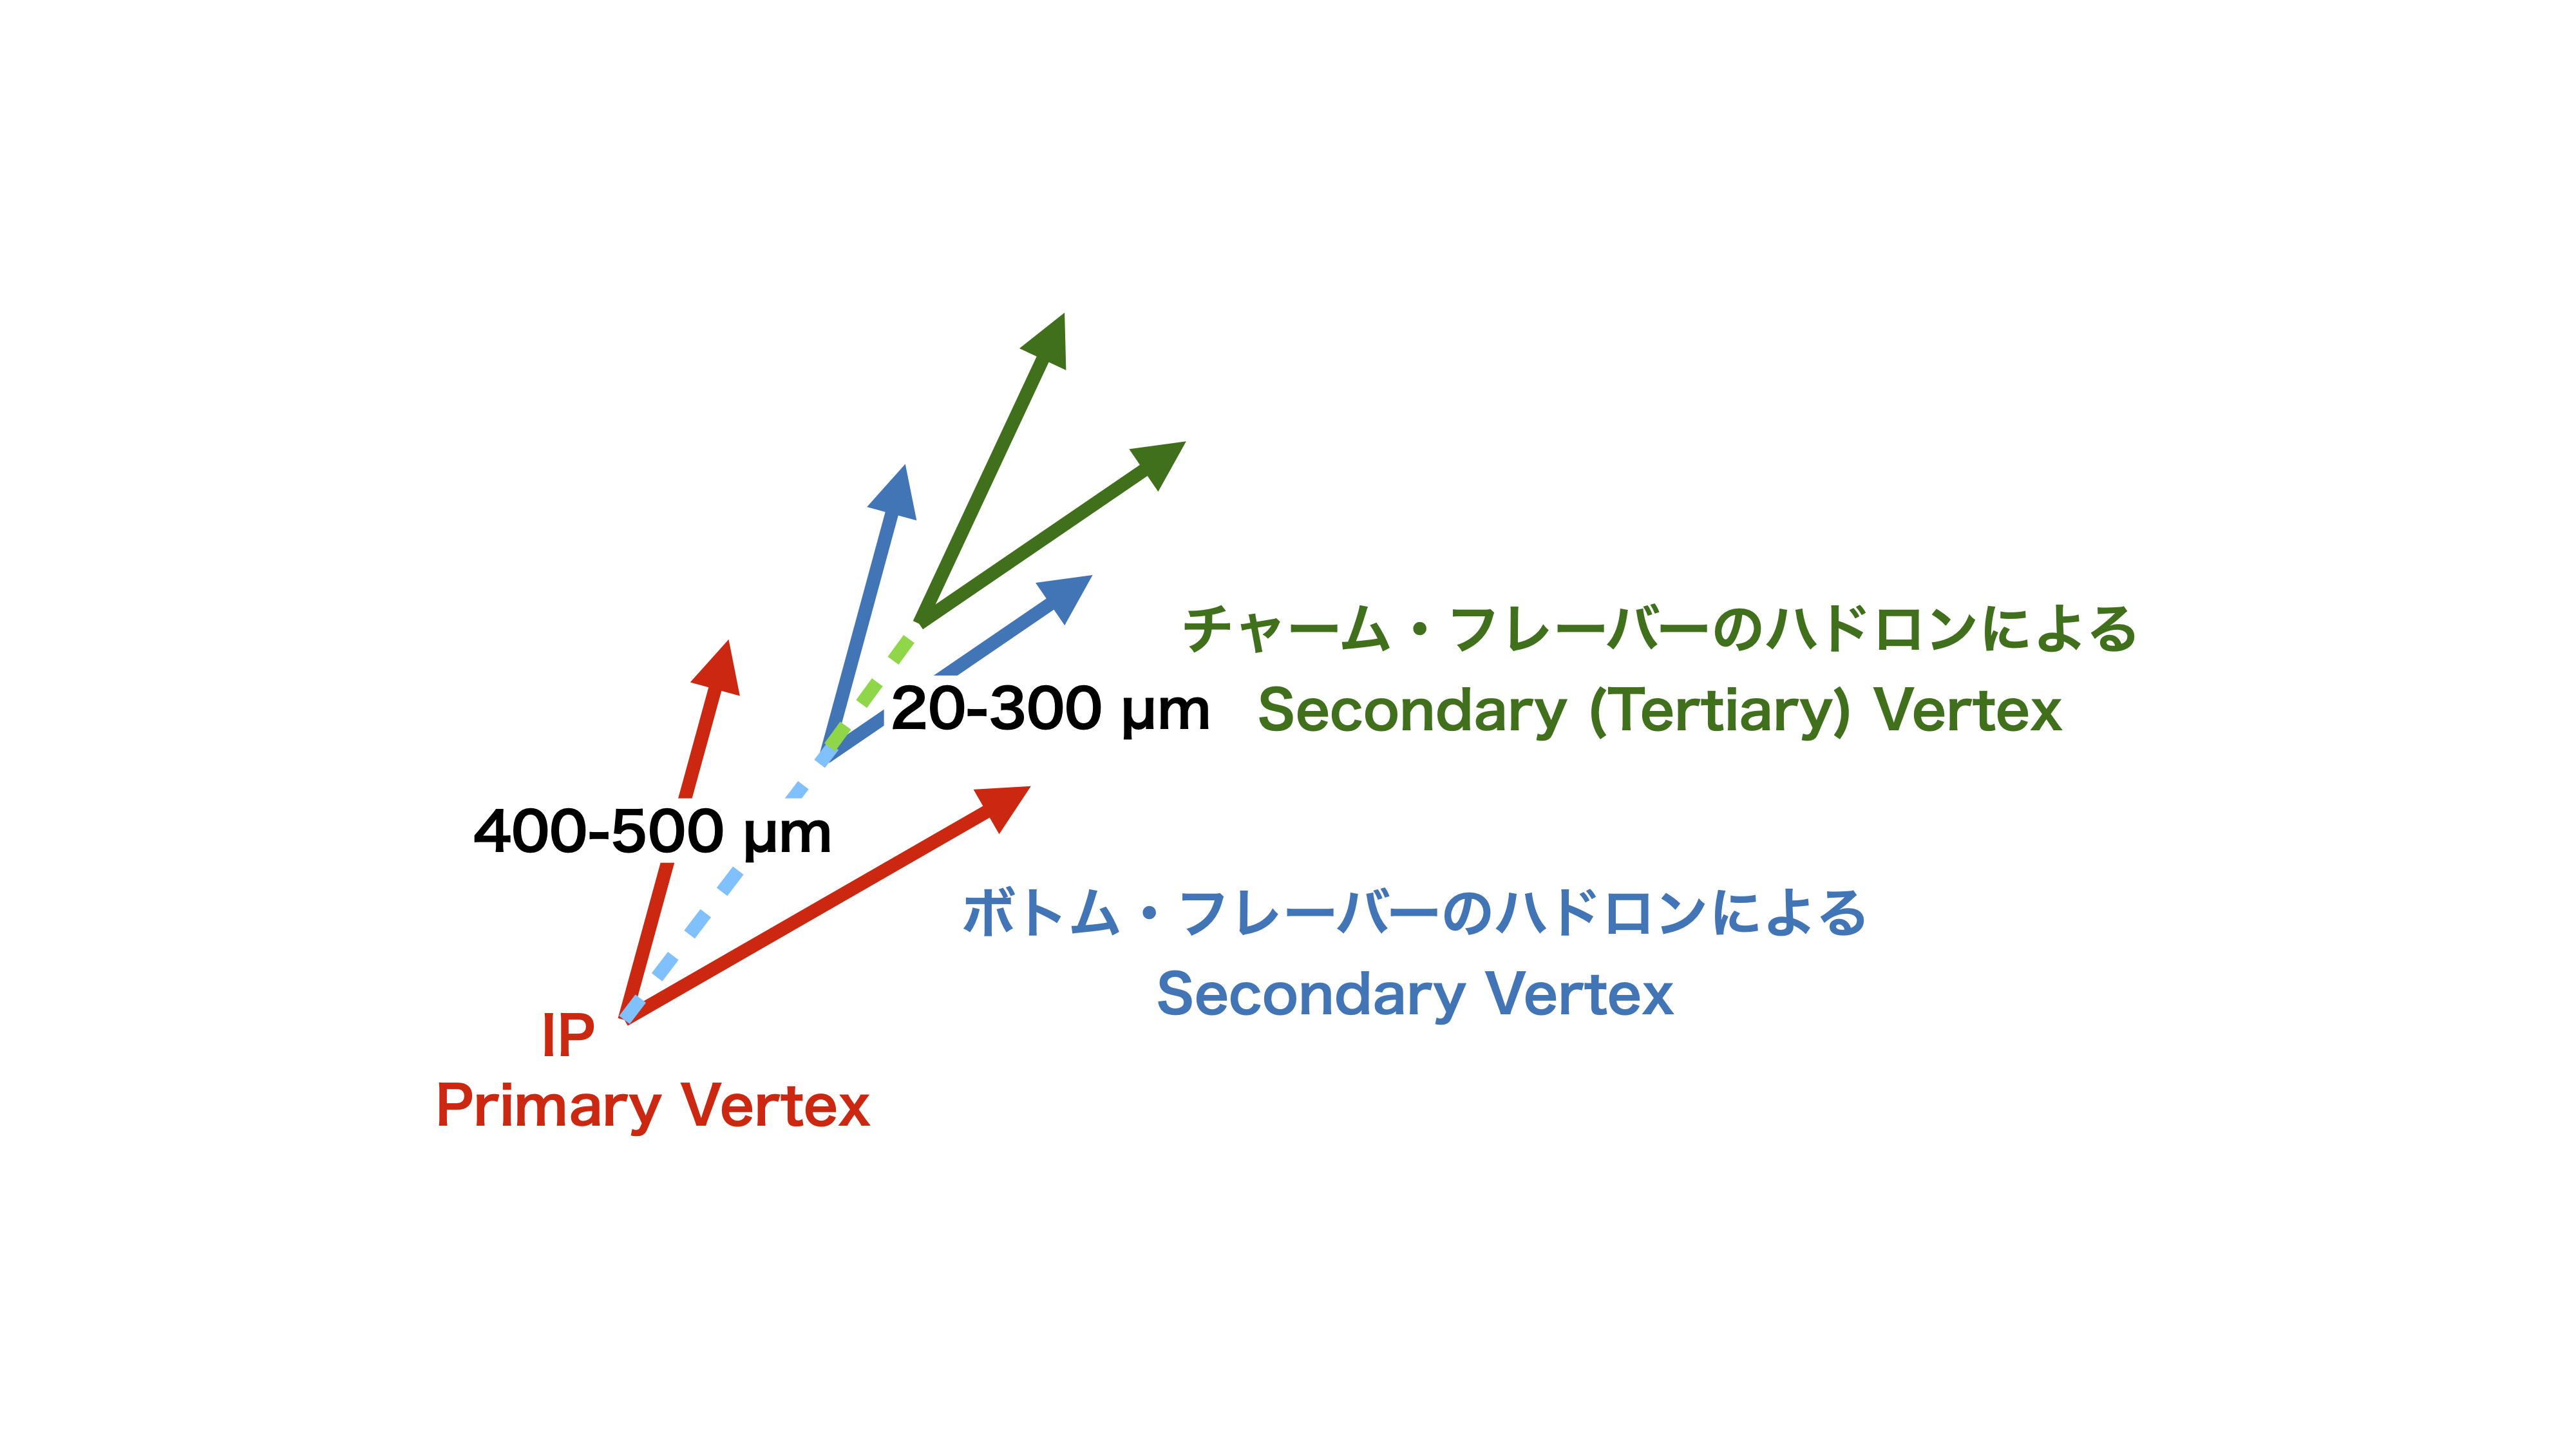
\includegraphics[trim = 200 200 200 200, width=0.9\textwidth, clip]{Figure/3Networks/3-1-1-1FinalStateBB.png}
 \caption[終状態$\rm b\bar{b}$での崩壊点の例]{終状態$\rm b\bar{b}$での崩壊点の例。赤線:Primary Vertex由来の飛跡。青線:Secondary Vertex由来の飛跡。緑線:Tertiary Vertex由来の飛跡。}
 \label{3-1-1-1FinalStateBB}
\end{figure}

また, これら以外の崩壊点としてタウ粒子の崩壊や$\rm V^0$粒子の崩壊 ($\rm K^0_S \to \pi^+\pi^-,\ \Lambda^0 \to p \pi^-$) , 光子変換 ($\rm \gamma_{conv} X \to e^+e^-X$) によるものを考えることができる。
これらの崩壊点はSecondary VertexやTertiary Vertexと比較して, 衝突点から遠い位置で生じる。
そのような崩壊点やその崩壊点由来の飛跡を以後Othersと呼ぶ。
図\ref{3-1-1-2TracksandVertices}は一つの事象に含まれる飛跡の本数と崩壊点の個数である。
これらの粒子識別はMC情報を用いた。
ここでは飛跡の本数は親粒子のフレーバーのみ考慮し, 同フレーバーの親粒子の違いは区別していない。
したがってSecondary Vertexについては, 一つの崩壊点ではなく$\rm b$と$\rm \bar{b}$などの複数の崩壊点の飛跡が含まれている。
親粒子の違いを区別しない場合のSecondary Vertexの飛跡の数は$5$本程度である。
本研究で使用したデータでは, 典型的な一事象に含まれる同フレーバーの崩壊点の数は$2$つである。
したがって個々のSecondary Vertexに含まれる飛跡の数は$2-3$本程度となる。
崩壊点検出ではPrimary Vertexと個々のSecondary Vertexを見分ける必要がある。

崩壊点の個数では親粒子を全て区別している。
典型的な崩壊点の個数は終状態が$\rm c\bar{c}$の場合はPrimary Vertex, チャーム・フレーバーのSecondary Vertexが$2$つ, Othersの$3-5$個である。
終状態が$\rm b\bar{b}$の場合はPrimary Vertex, ボトム・フレーバーのSecondary Vertexが$2$つ, チャーム・フレーバーのTertiary Vertexが$2$つ, Othersの$5-7$個である。

\begin{figure}[htbp]
 \centering
 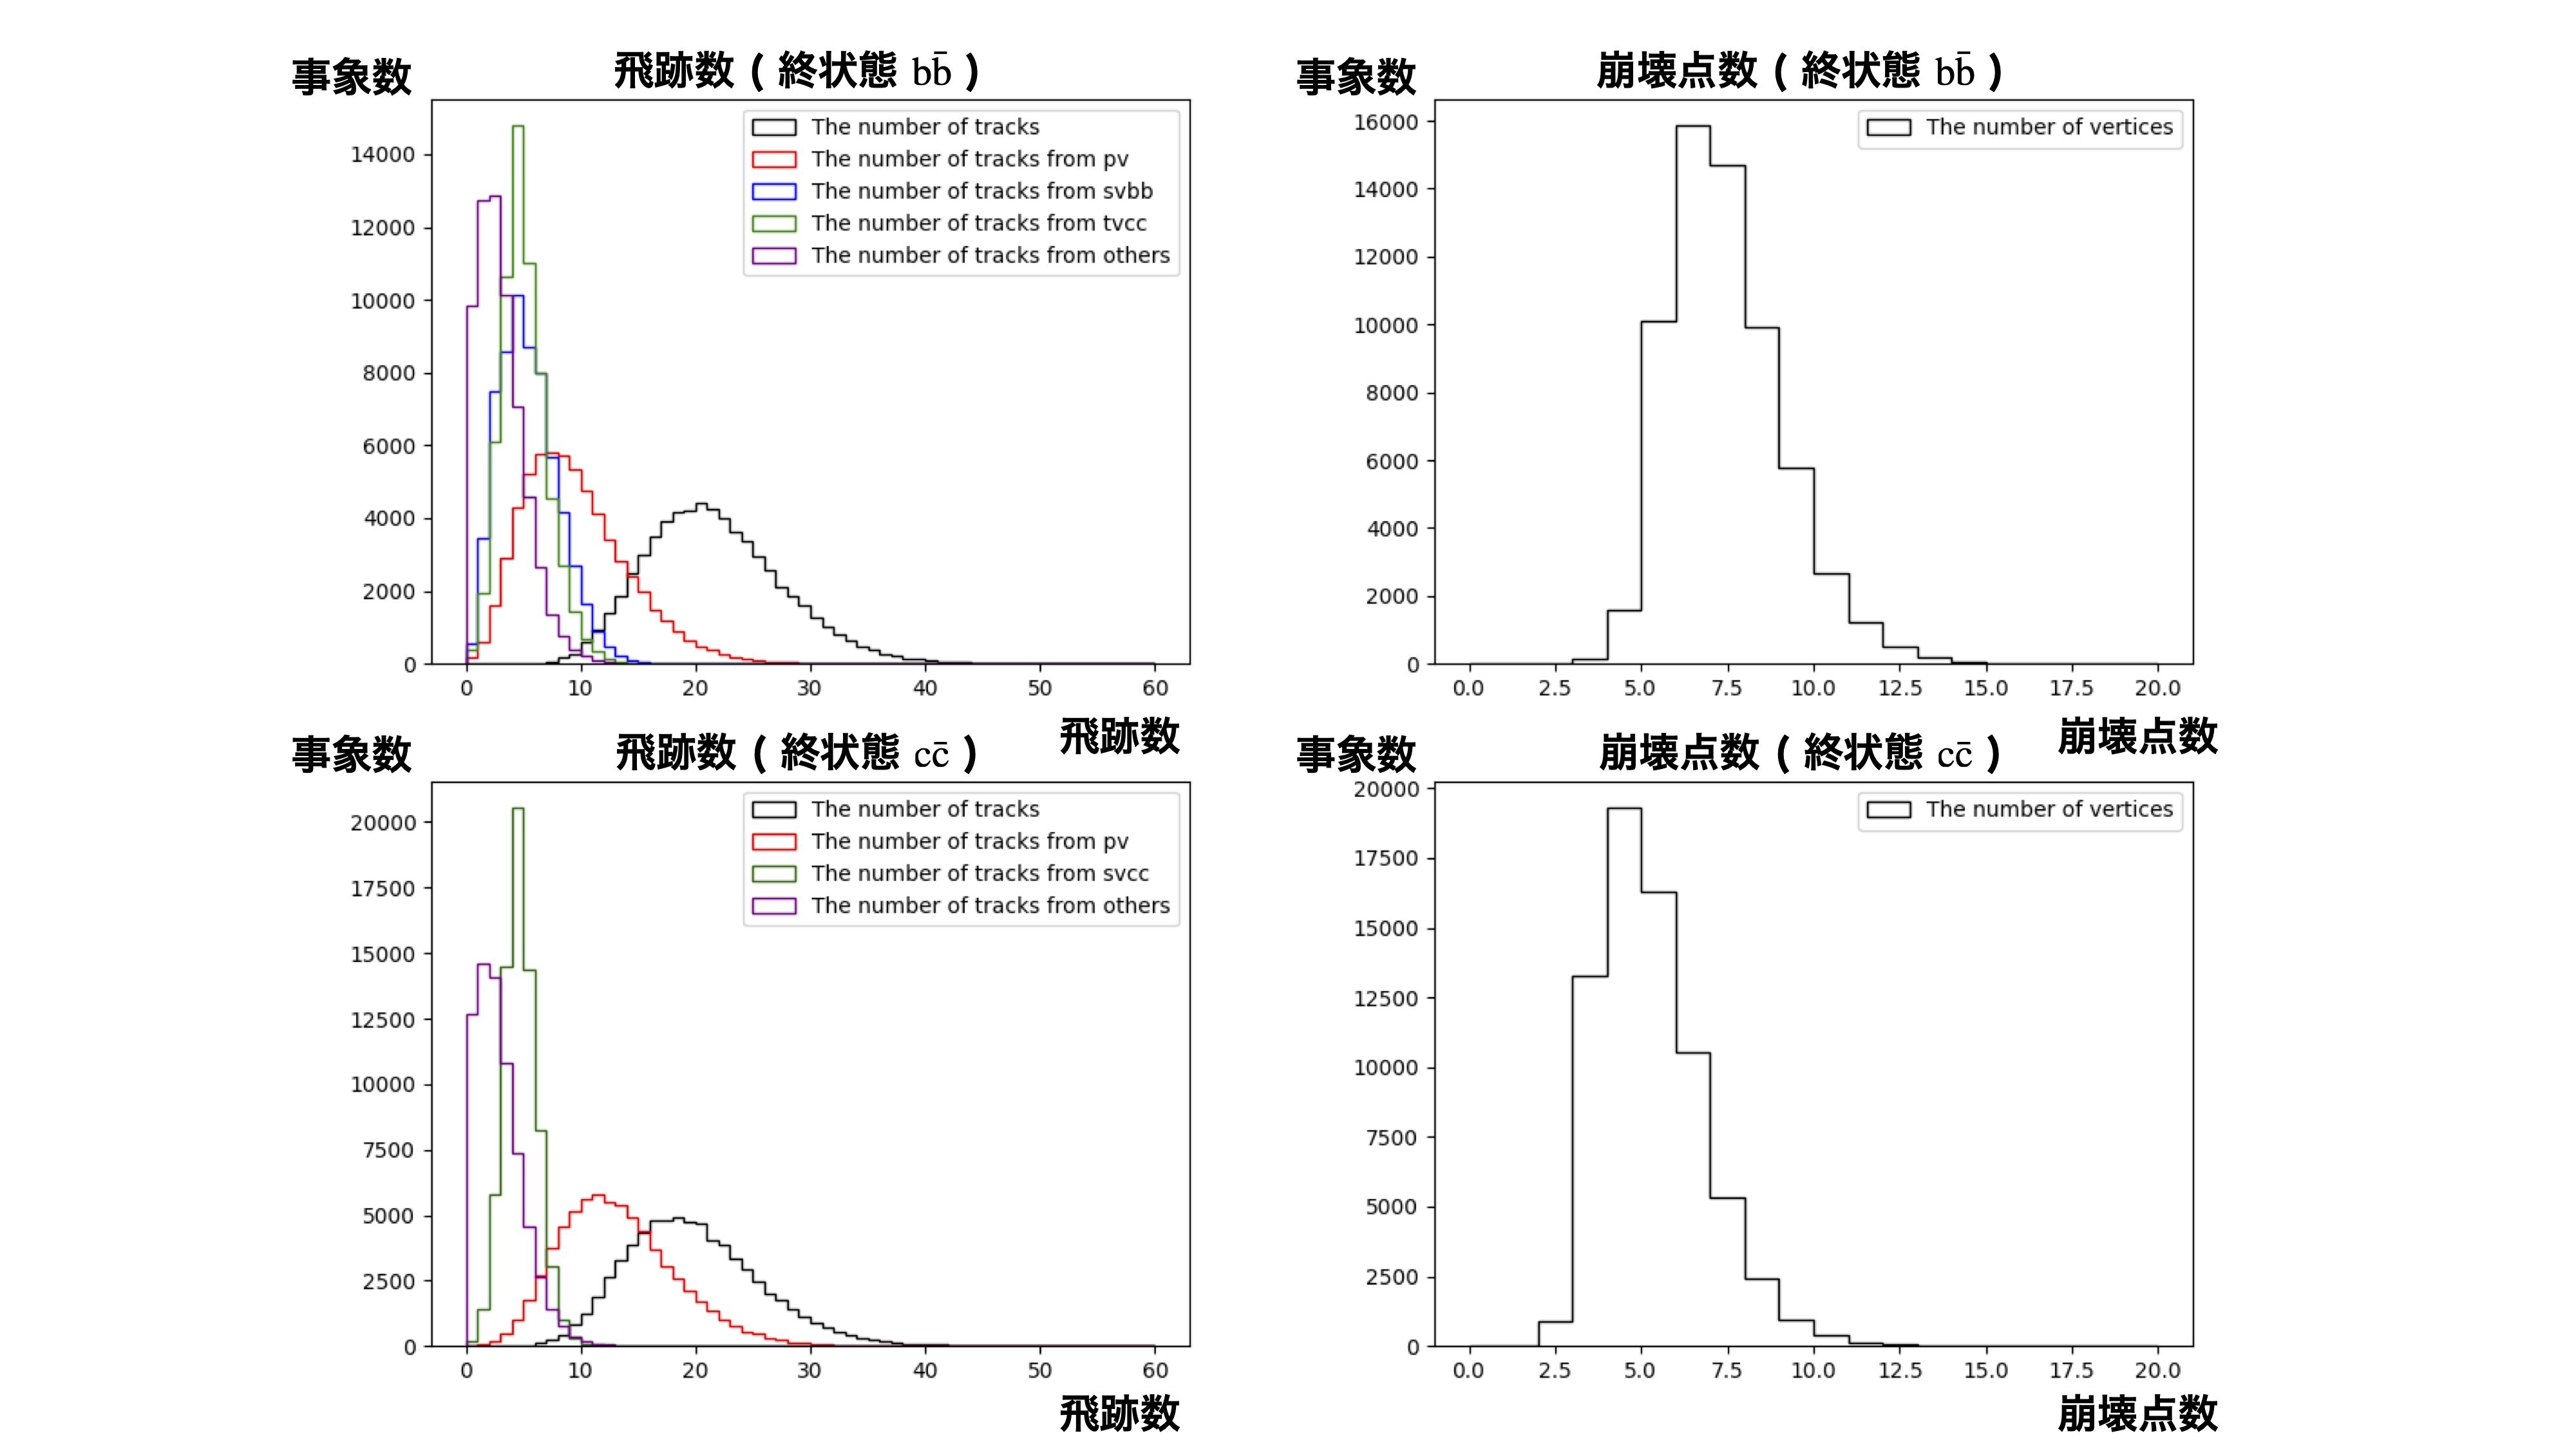
\includegraphics[trim = 150 0 150 0, width=1.0\textwidth, clip]{Figure/3Networks/3-1-1-2TracksandVertices.png}
 \caption[事象に含まれる飛跡の本数と崩壊点の個数]{事象に含まれる飛跡の本数と崩壊点の個数。図左は飛跡の本数, 図右は崩壊点の個数である。飛跡の本数において, 黒線は事象に含まれる全飛跡数, 赤線はPrimary Vertex由来の飛跡数, 青線はボトム・フレーバーのSecondary Vertex由来の飛跡数, 緑線はチャーム・フレーバーのSecondary Vertex由来の飛跡数, 紫線はOthersの飛跡数を表している。}
 \label{3-1-1-2TracksandVertices}
\end{figure}


%%%%%%%%%%%%%%%%%%%%%%%%%%%%%%%%%%%%%%%%%%%%%%%%%%%%%%%%%%%%%%%%%%%%%%%%
\subsection{飛跡の情報と前処理} \label{Net:Data:TrackInformationandPreprocessing}

飛跡一本分の情報として, 図\ref{3-1-2-1TrackParameters}のような位置や運動量の情報を含んだトラック・パラメータ$5$個 ($\rm d_0$, $\rm z_0$, $\rm \phi$, $\rm \Omega$, $\rm \tan{\lambda}$)\cite{TrackParametersLCIO}とその共分散行列$15$個, 電荷, エネルギーの計$22$個の変数を使用した。
また, 加速器の座標系としてビーム衝突点を原点とし, Z軸をビーム方向にとった座標系を使用する。

\begin{figure}[htbp]
 \centering
 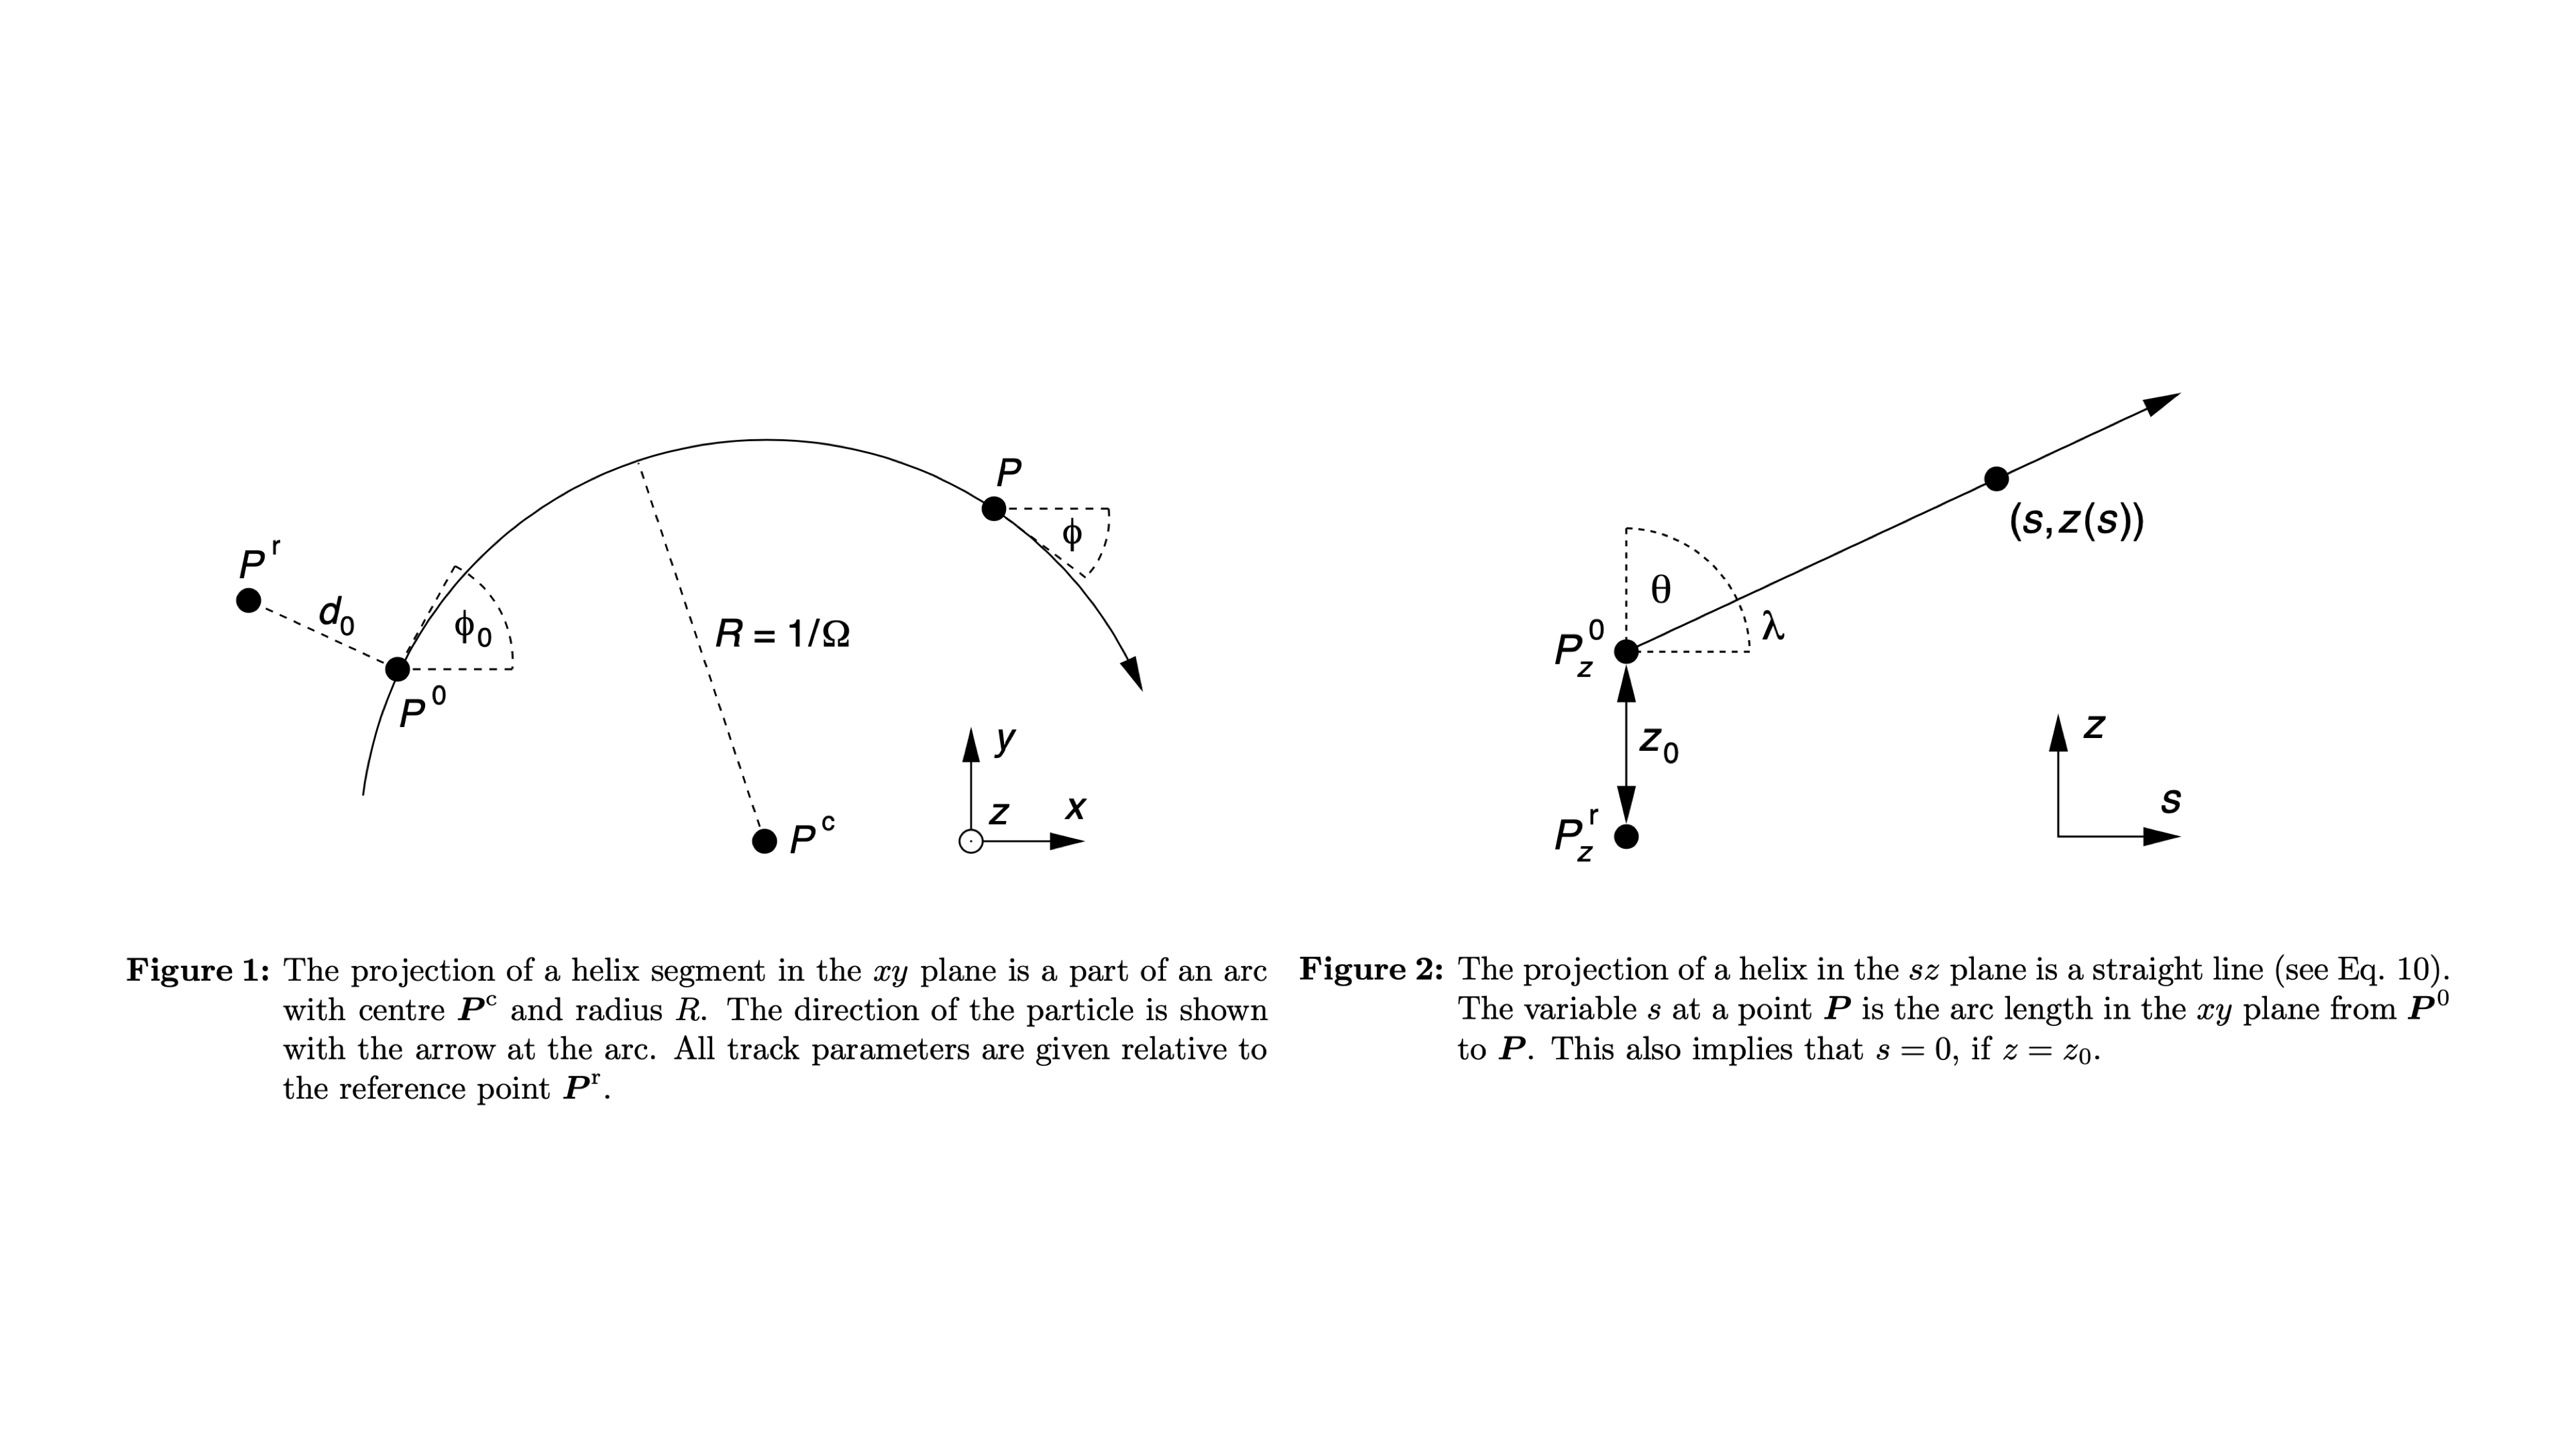
\includegraphics[trim = 50 150 50 250, width=1.0\textwidth, clip]{Figure/3Networks/3-1-2-1TrackParameters.png}
 \caption[トラック・パラメータの定義]{トラック・パラメータの定義\cite{TrackParametersLCIO}}
 \label{3-1-2-1TrackParameters}
\end{figure}

深層学習の入力に使用する変数は, 一般に$[-1,\ 1]$の範囲に整形した方が良いと言われている為, 変数をそれぞれ以下のような$\tanh$関数や線形関数などを用いて整形した。

\begin{itemize}
 \item トラック・パラメータ\\
 ${\rm d_0} = \tanh{({\rm d_0})}$,
 ${\rm z_0} = \tanh{({\rm z_0})}$,
 ${\rm \phi} = {\rm \phi}/\pi$,
 ${\rm \Omega} = \tanh{(200\ {\rm \Omega})}$,
 ${\rm \tan{\lambda}} = \tanh{(0.3\ {\rm \tan{\lambda}})}$
 \item トラック・パラメータの共分散行列\\
 $\tanh{(8000\ (x-0.0005))}$
 \item エネルギー\\
 $\tanh{(0.5\ (x-5.0))}$
\end{itemize}

トラック・パラメータとエネルギーの整形前と整形後の分布をそれぞれ図\ref{3-1-2-2Variables}に示す。
整形後の変数の分布が$[-1,\ 1]$の範囲になっていることがわかる。

\begin{figure}[htbp]
 \centering
  %\begin{tabular}{cccc}
  \begin{minipage}{1.0\textwidth}
  \centering
   \begin{minipage}{0.48\textwidth}
    \centering
    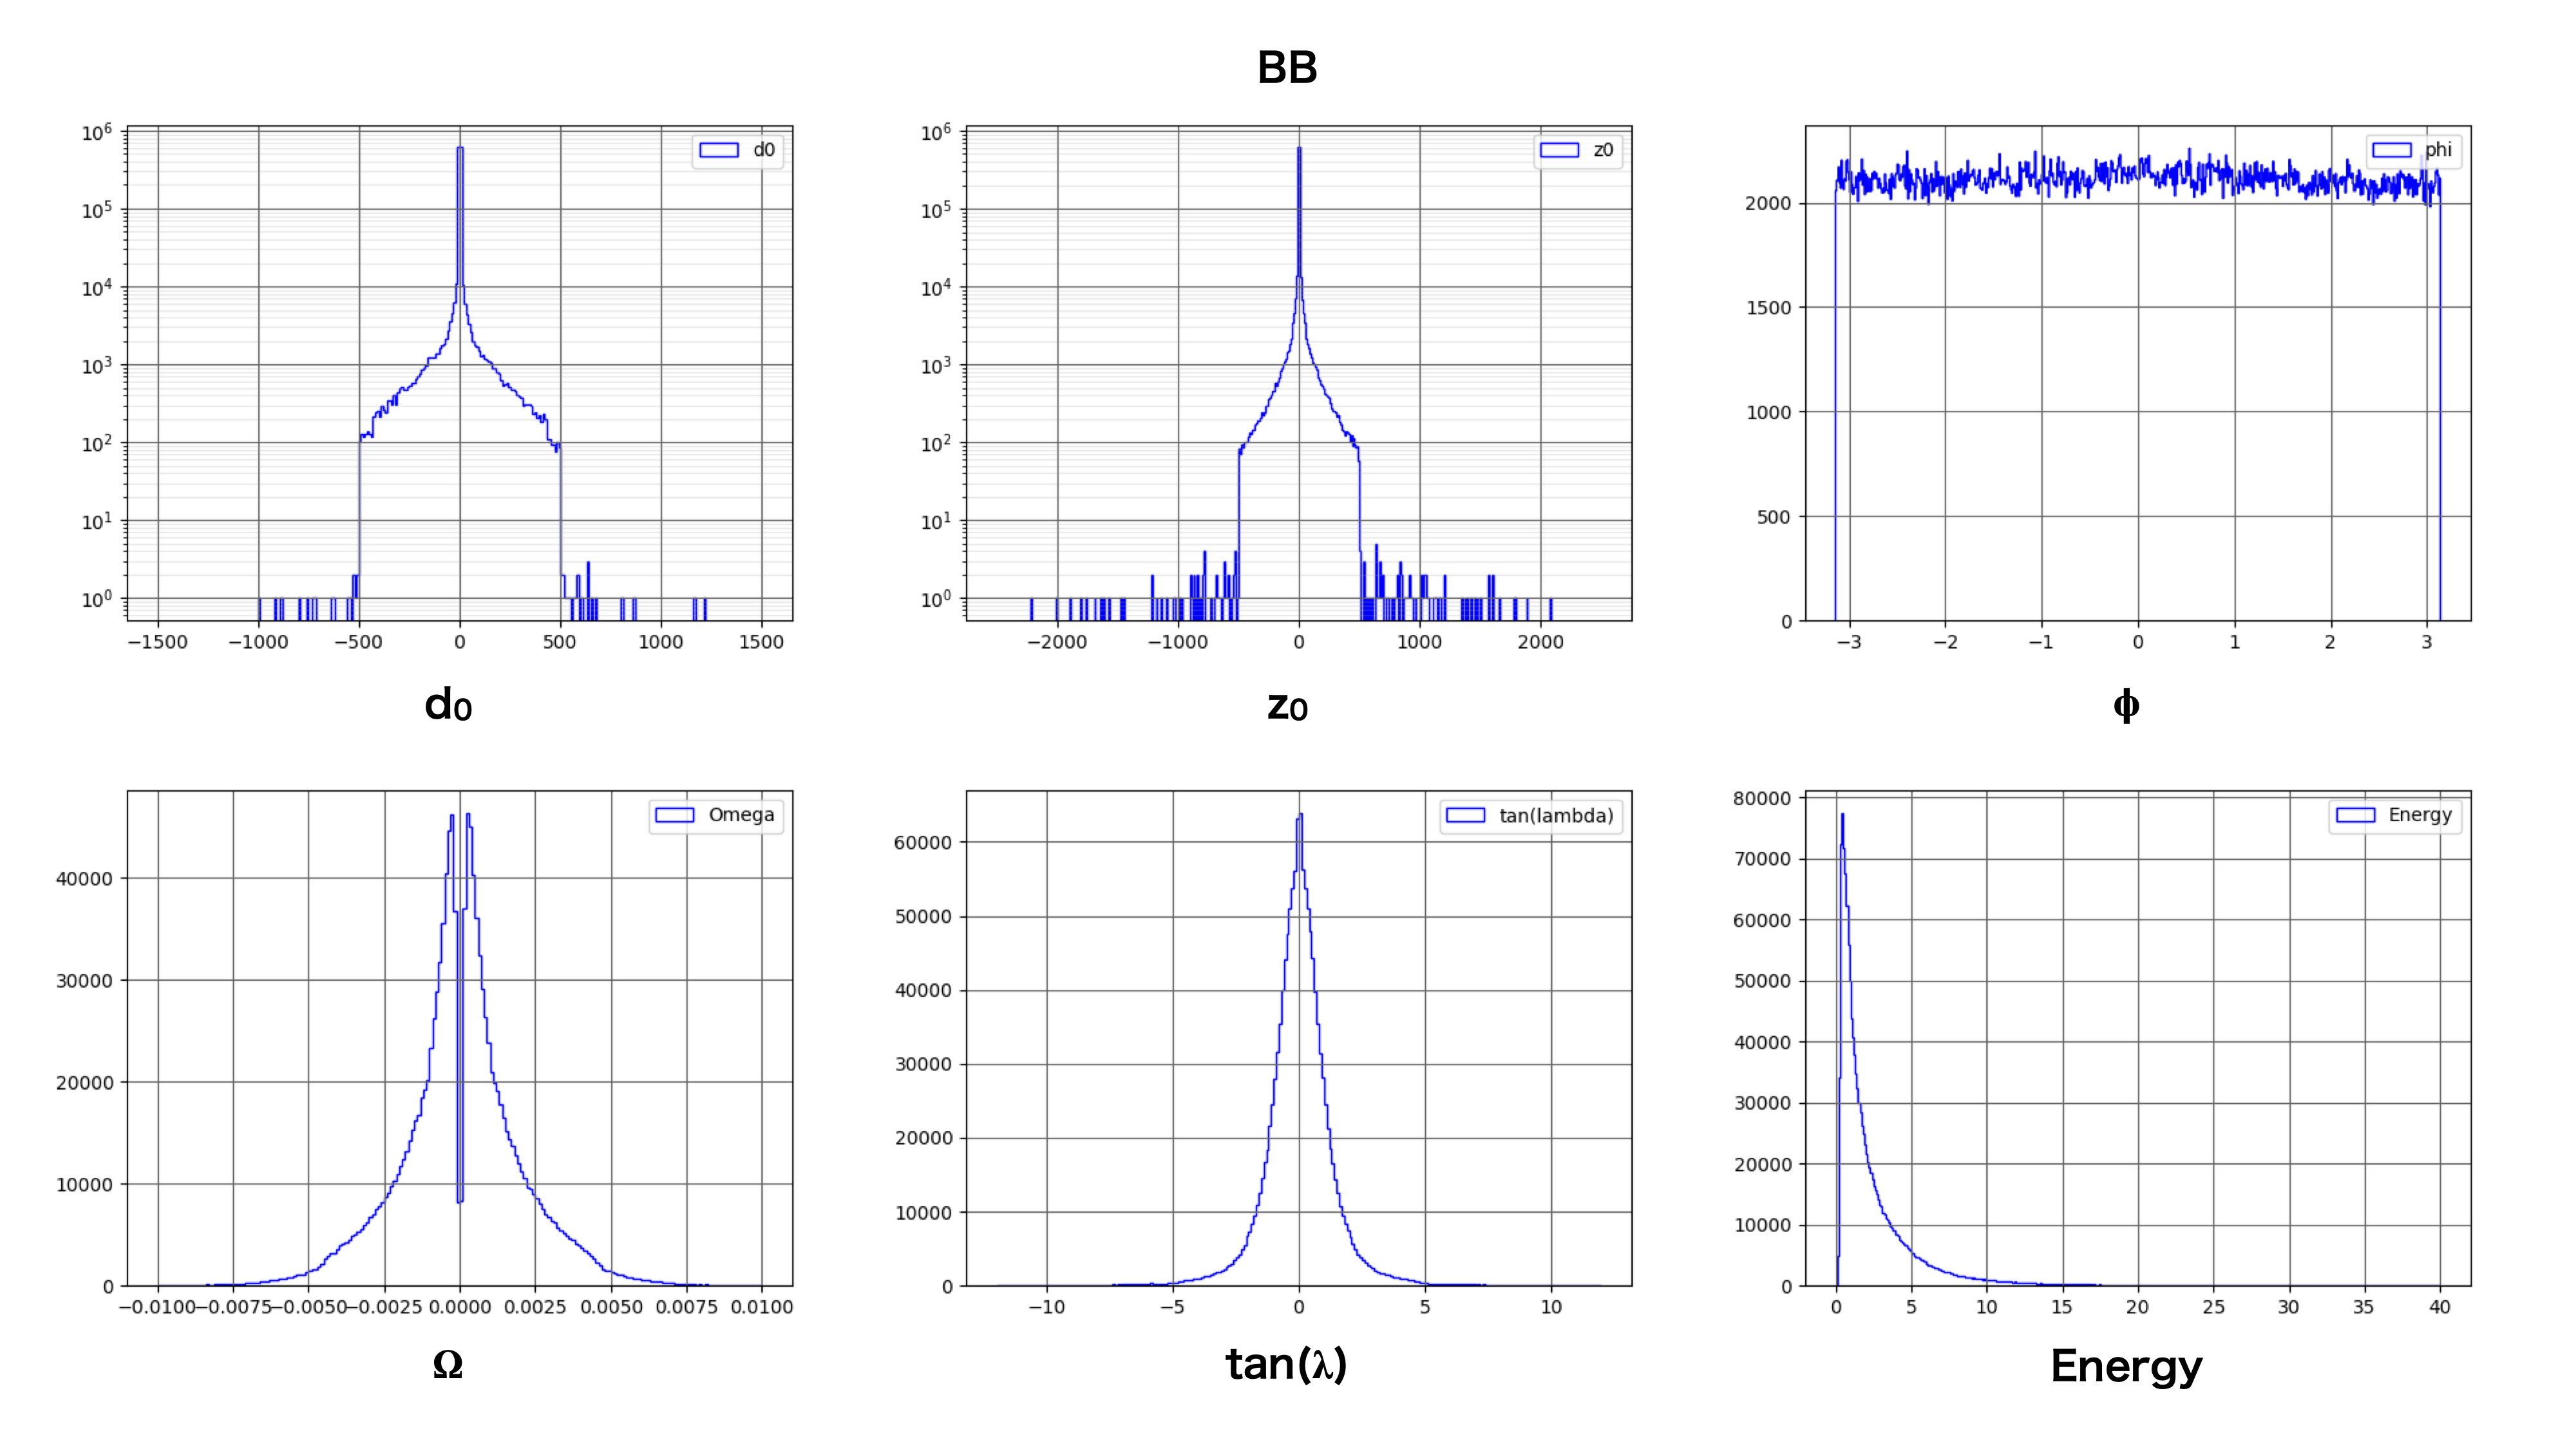
\includegraphics[width=1.0\textwidth, clip]{Figure/3Networks/3-1-2-2OriginalVariablesBB.png}
    \subcaption{終状態$\rm b\bar{b}$での変換前の変数の分布}
    \label{3-1-2-2OriginalVariablesBB}
   \end{minipage}
   \begin{minipage}{0.48\textwidth}
   \centering
    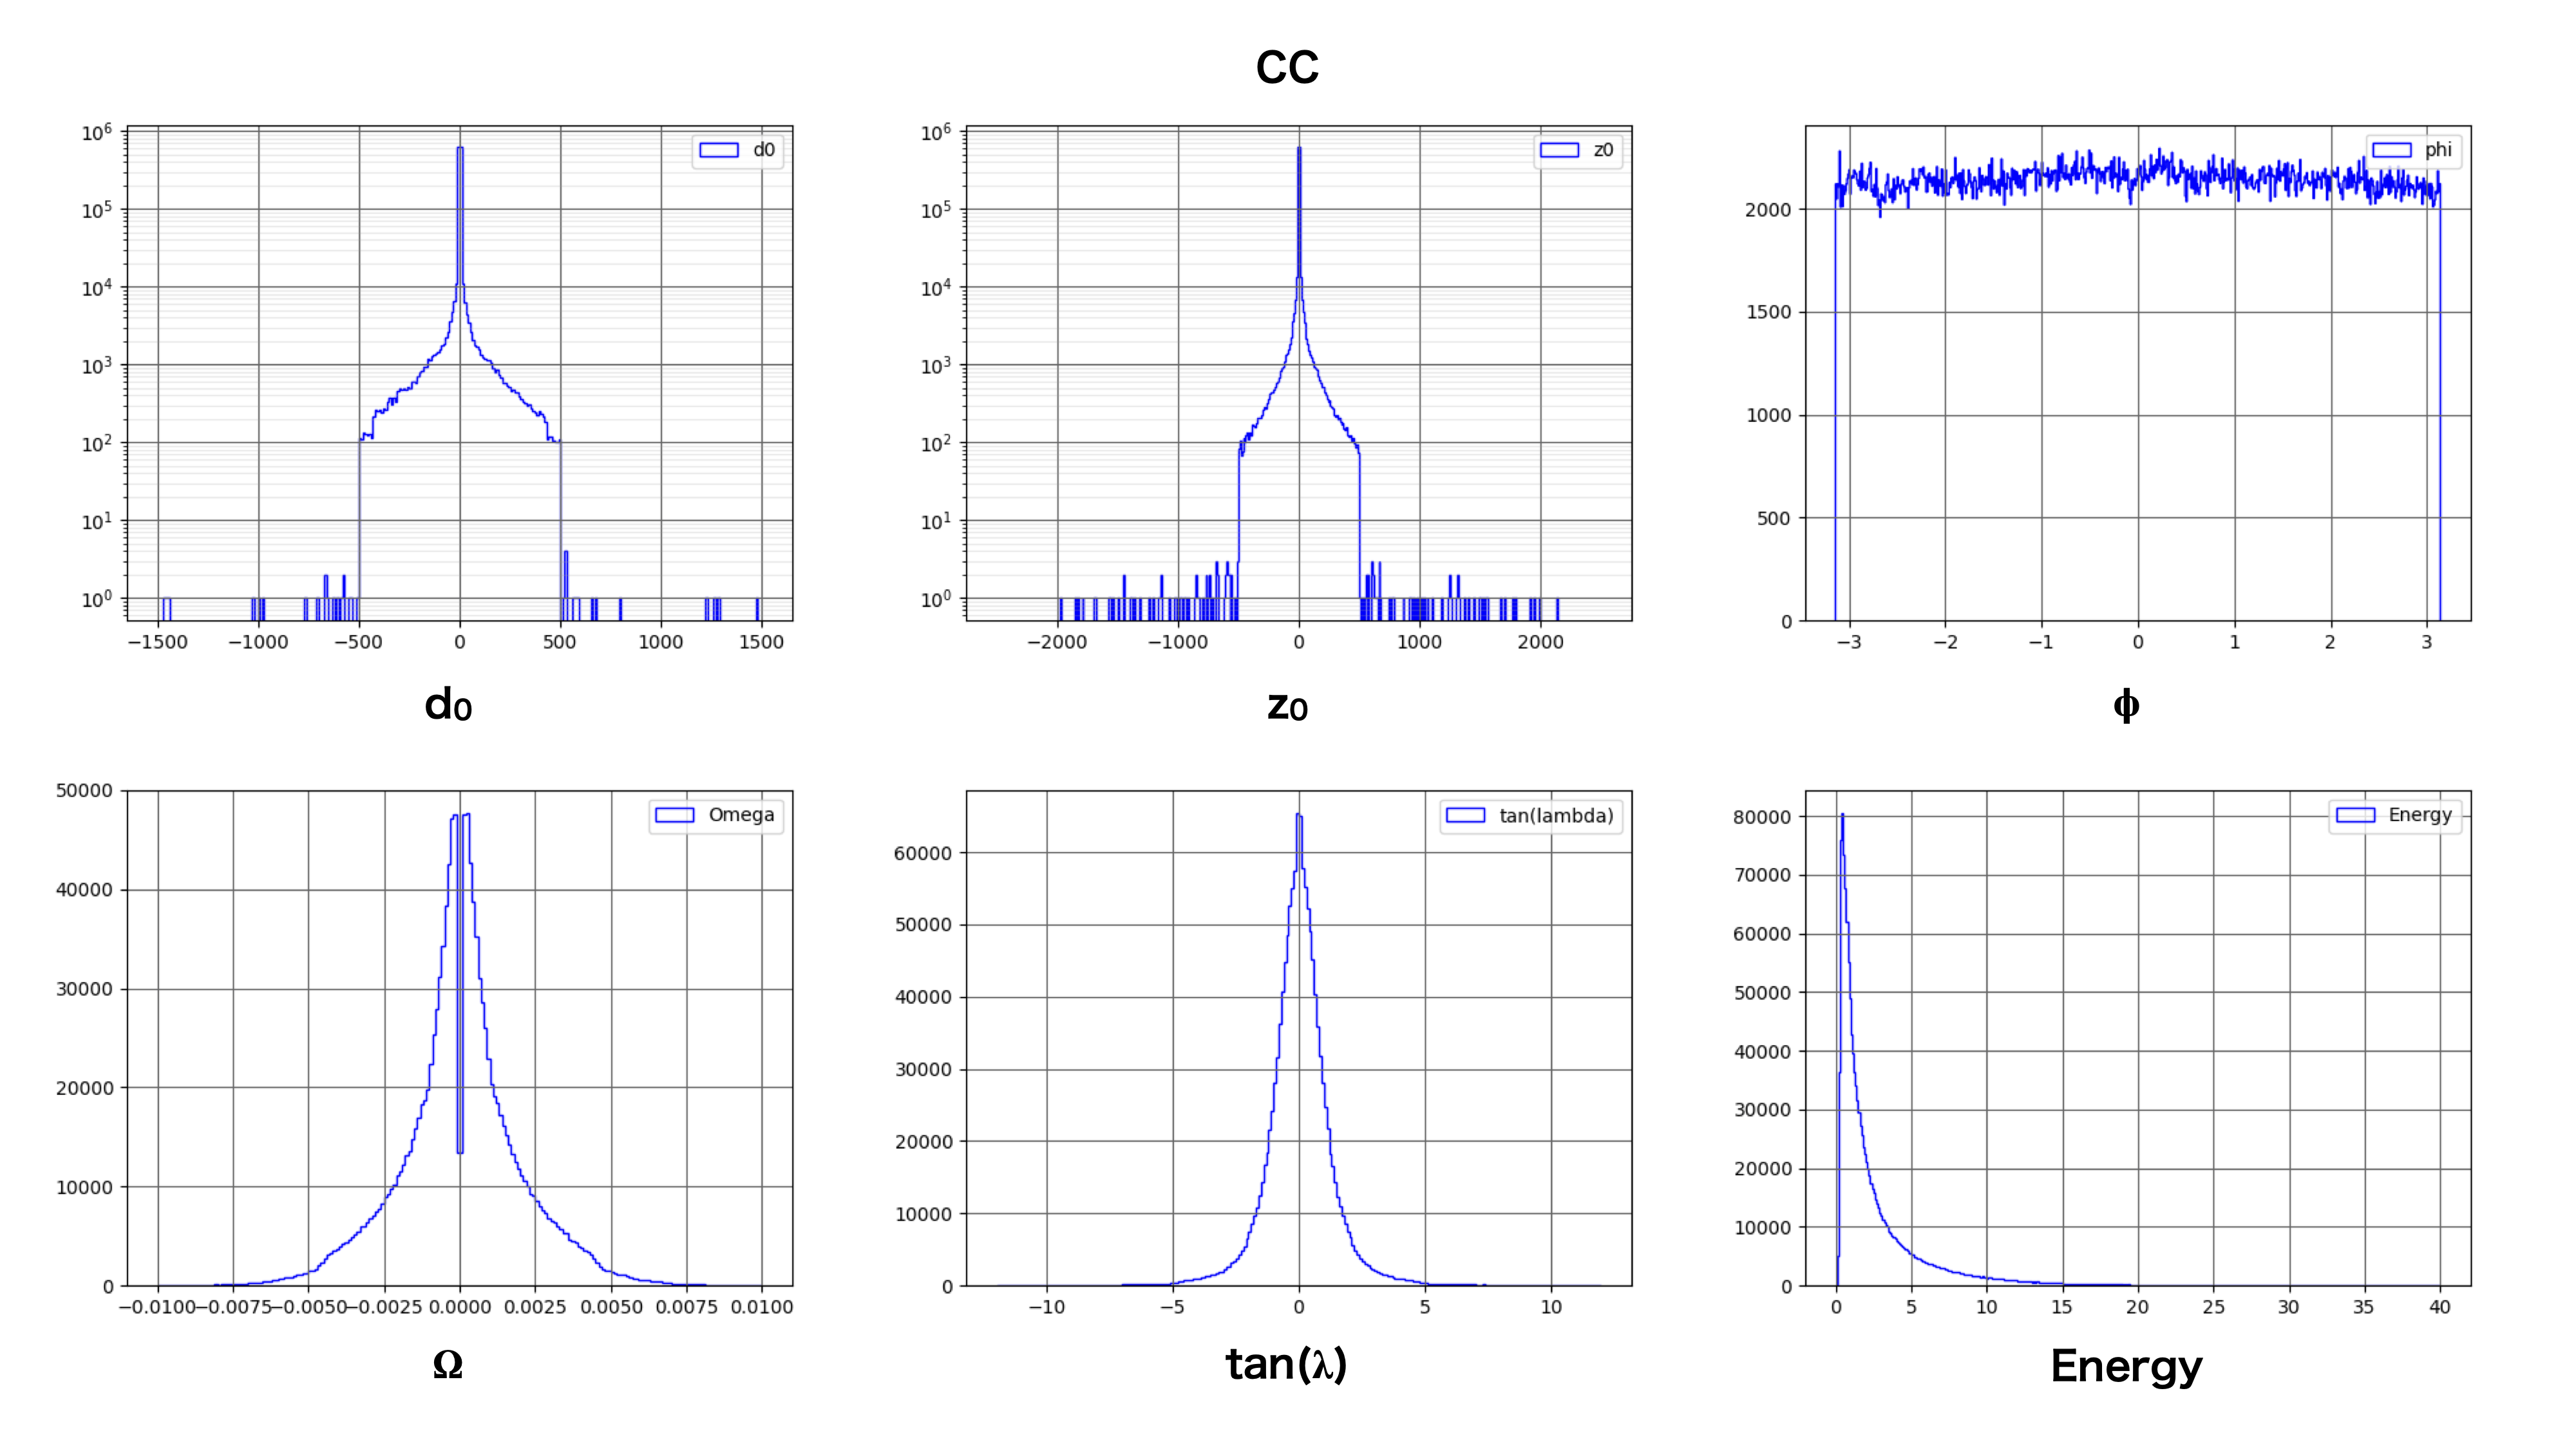
\includegraphics[width=1.0\textwidth, clip]{Figure/3Networks/3-1-2-2OriginalVariablesCC.png}
    \subcaption{終状態$\rm c\bar{c}$での変換前の変数の分布}
    \label{3-1-2-2OriginalVariablesCC}
   \end{minipage}
  \end{minipage}
  
  \begin{minipage}{1.0\textwidth}
  \centering
   \begin{minipage}{0.48\textwidth}
   \centering
    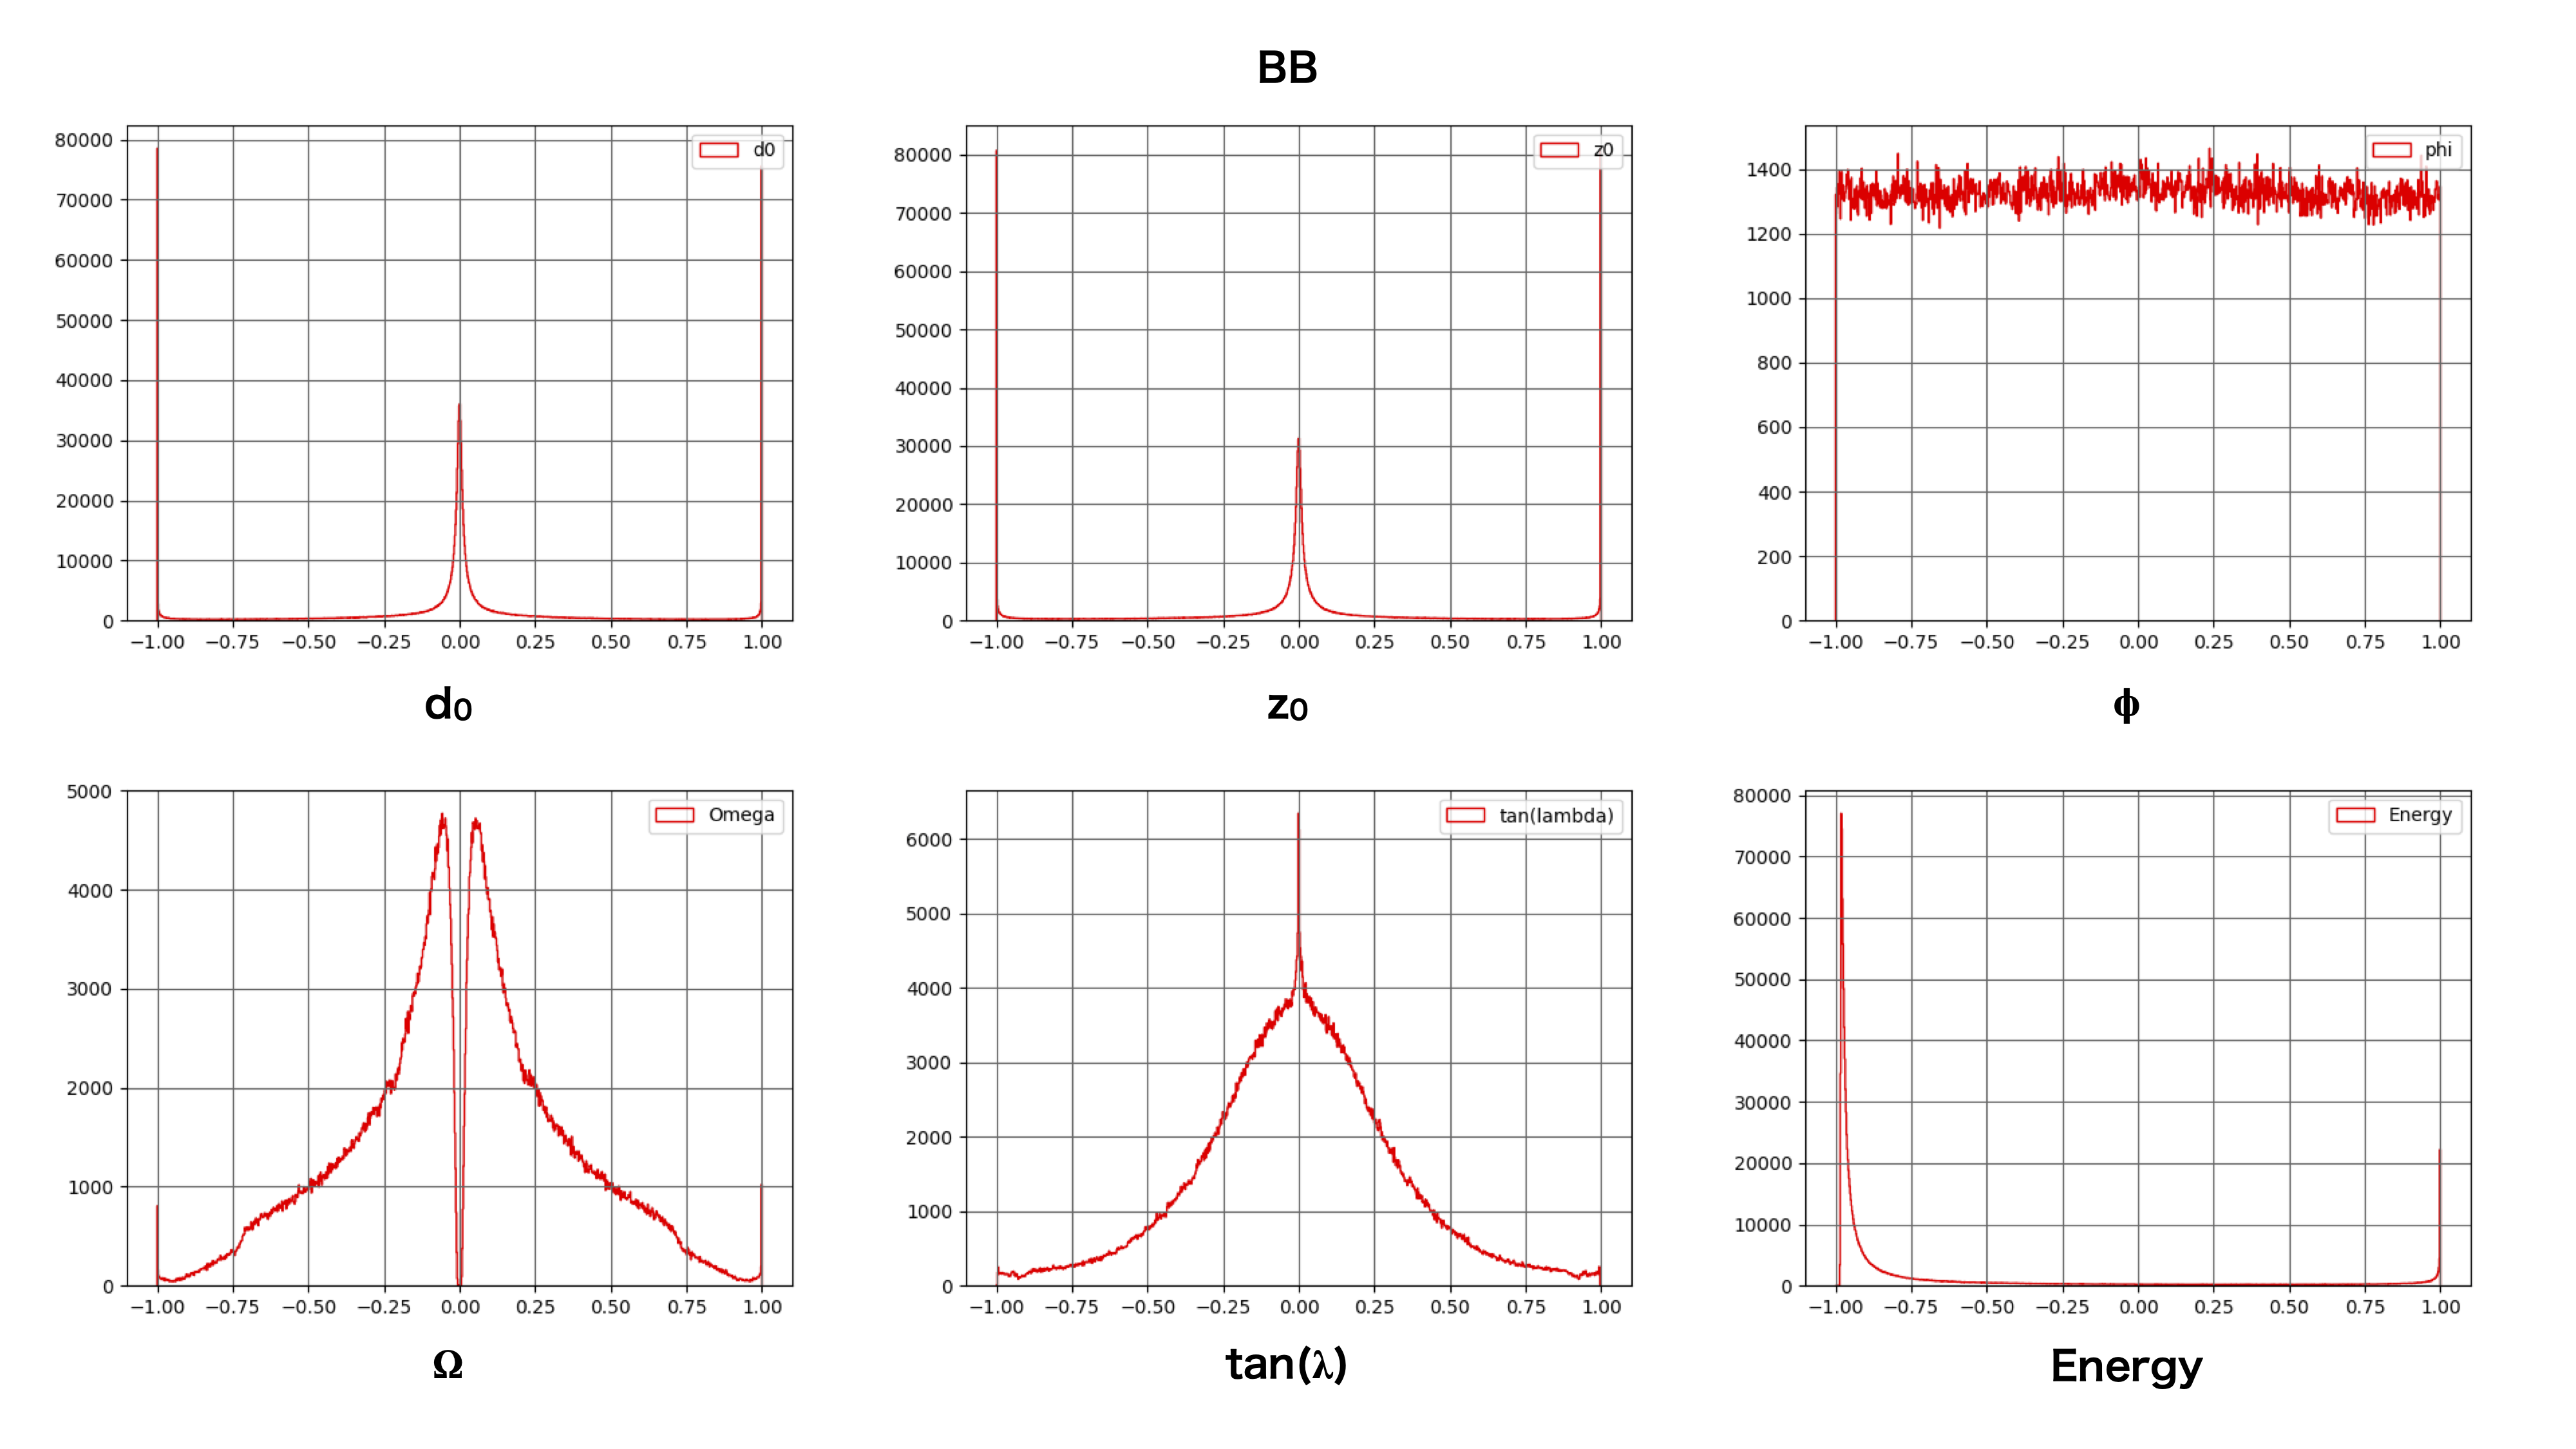
\includegraphics[width=1.0\textwidth, clip]{Figure/3Networks/3-1-2-2ReshapedVariablesBB.png}
    \subcaption{終状態$\rm b\bar{b}$での変換後の変数の分布}
    \label{3-1-2-2ReshapedVariablesBB}
   \end{minipage}
   \begin{minipage}{0.48\textwidth}
   \centering
    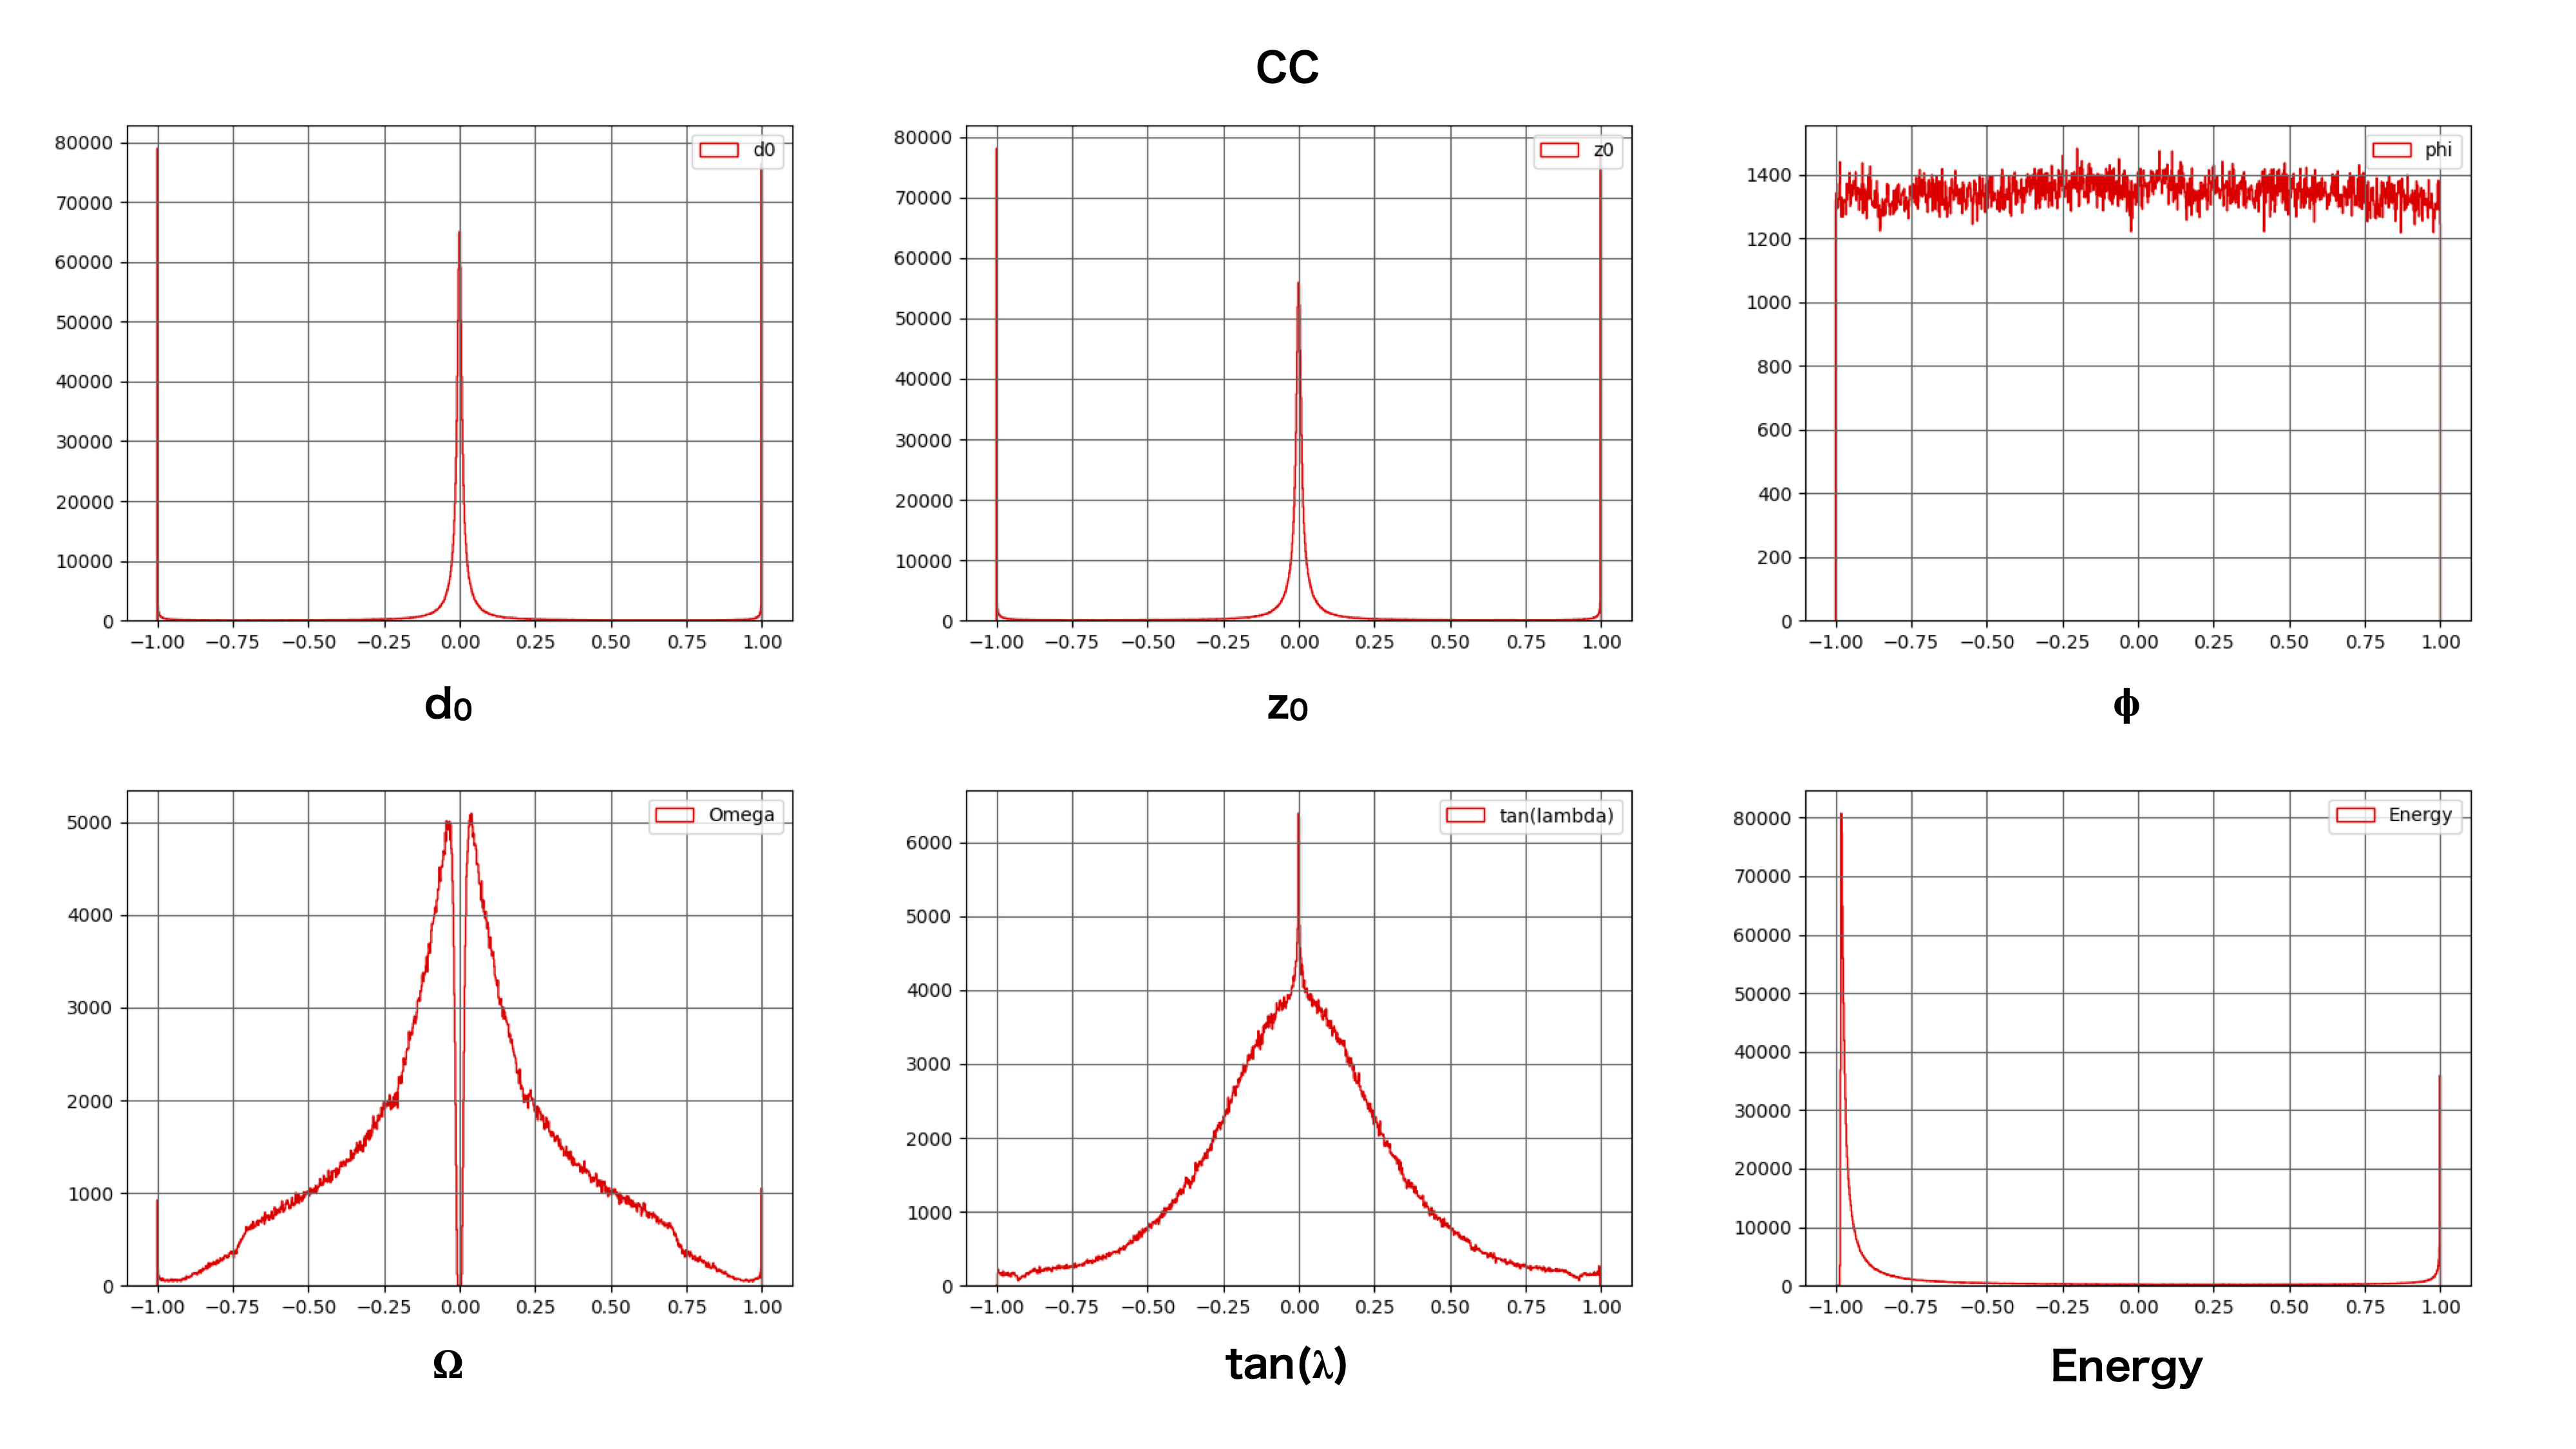
\includegraphics[width=1.0\textwidth, clip]{Figure/3Networks/3-1-2-2ReshapedVariablesCC.png}
    \subcaption{終状態$\rm c\bar{c}$での変換後の変数の分布}
    \label{3-1-2-2ReshapedVariablesCC}
   \end{minipage}
   \end{minipage}
  \caption{変数の分布の例}
  \label{3-1-2-2Variables}
 %\end{tabular}
\end{figure}

また, LCFIPlusのフィッティングで得られる$\chi^2$や崩壊点の位置についてもデータを用意した。
ここでは, 事象中の二本の飛跡 (飛跡対) の全ての組み合わせについて計算を行った。
ただし, このような高次の情報を含んだ変数は基本的にはネットワークの学習に使用せず, 正解ラベルの一つとして使用した。
LCFIPlusによって予想される崩壊点の位置について, ビーム衝突点からの距離を図\ref{3-1-2-3VertexPositions}に示す。
図\ref{3-1-2-3VertexPositions}のグラフは両対数グラフとして表現している為, 衝突点からの距離$10^{-2}\ \mathrm{mm}$から$10^{3}\ \mathrm{mm}$のプロットとなっており, 衝突点は含んでいない。
Primary VertexとSecondary Vertexの衝突点からの距離は大きく異なっているが, 各フレーバーのSecondary Vertexの衝突点からの距離は殆ど離れていないことが分かる。
また, 終状態$\rm c\bar{c}$と終状態$\rm b\bar{b}$では$\rm b \to c$の崩壊過程を辿るか否かの違いがある為, チャーム・フレーバーの崩壊点の位置が少し異なっている。
Othersは衝突点付近では殆ど起こらず, 他の崩壊点と比較して遠い位置で崩壊している。
このように崩壊点検出において位置の再構成は非常に重要な情報を含んでおり, 逆説的に位置の再構成が出来なければ崩壊点に分離は困難であると言える。

\begin{figure}[htbp]
 \centering
 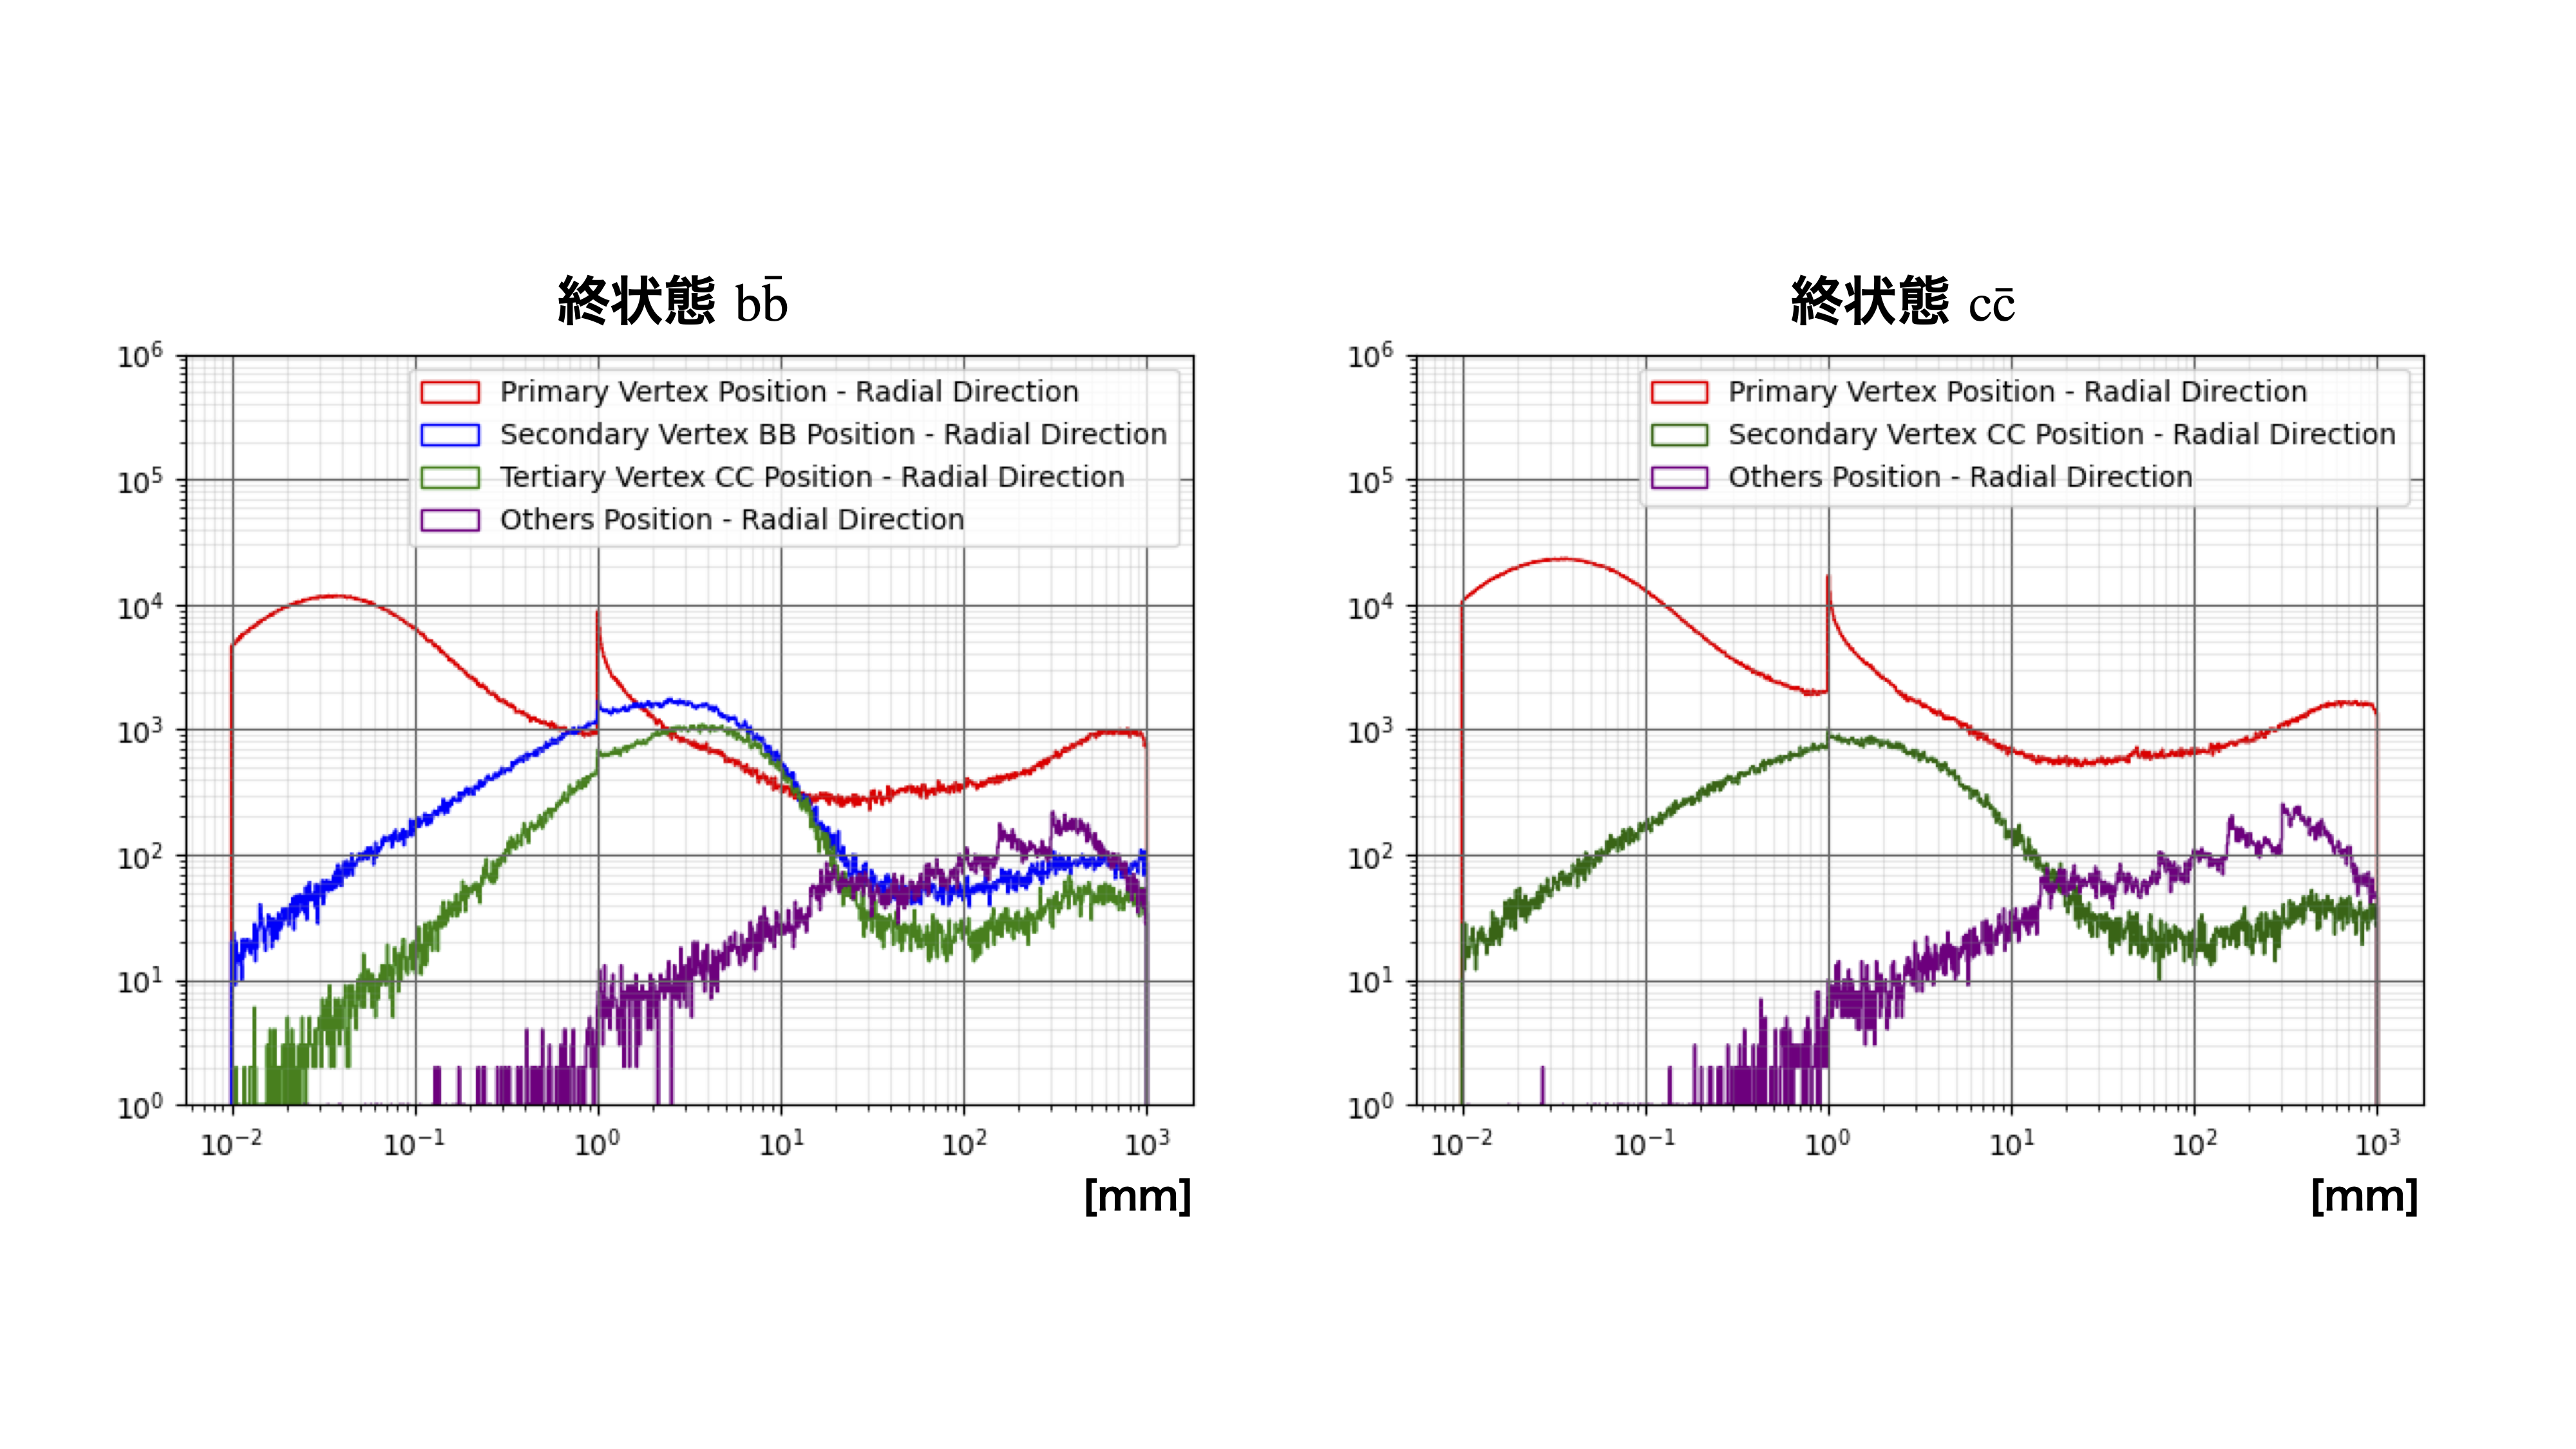
\includegraphics[trim = 50 100 50 150, width=1.0\textwidth, clip]{Figure/3Networks/3-1-2-3VertexPositions.png}
 \caption[LCFIPlusによって予想される崩壊点の位置の分布]{LCFIPlusによって予想される崩壊点の位置の分布。横軸はログスケールの衝突点からの距離である。赤線はPrimary Vertexの位置, 青線はボトム・フレーバーのSecondary Vertexの位置, 緑線はチャーム・フレーバーのSecondary Vertexの位置, 紫線はOthersの位置を表している。これらは飛跡対についてのLCFIPlusの計算値である。}
 \label{3-1-2-3VertexPositions}
\end{figure}

$1\ \mathrm{mm}$付近のピークはLCFIPlusのフィッティングが失敗している飛跡対である。
フィッティング健全性を表す$\chi^2$との相関を見ると, 図\ref{3-1-2-4VertexPositionsvsChiSquare}のように, $1\ \mathrm{mm}$付近のデータは大きな$\chi^2$値を持っていることが分かる。

\begin{figure}[htbp]
 \centering
 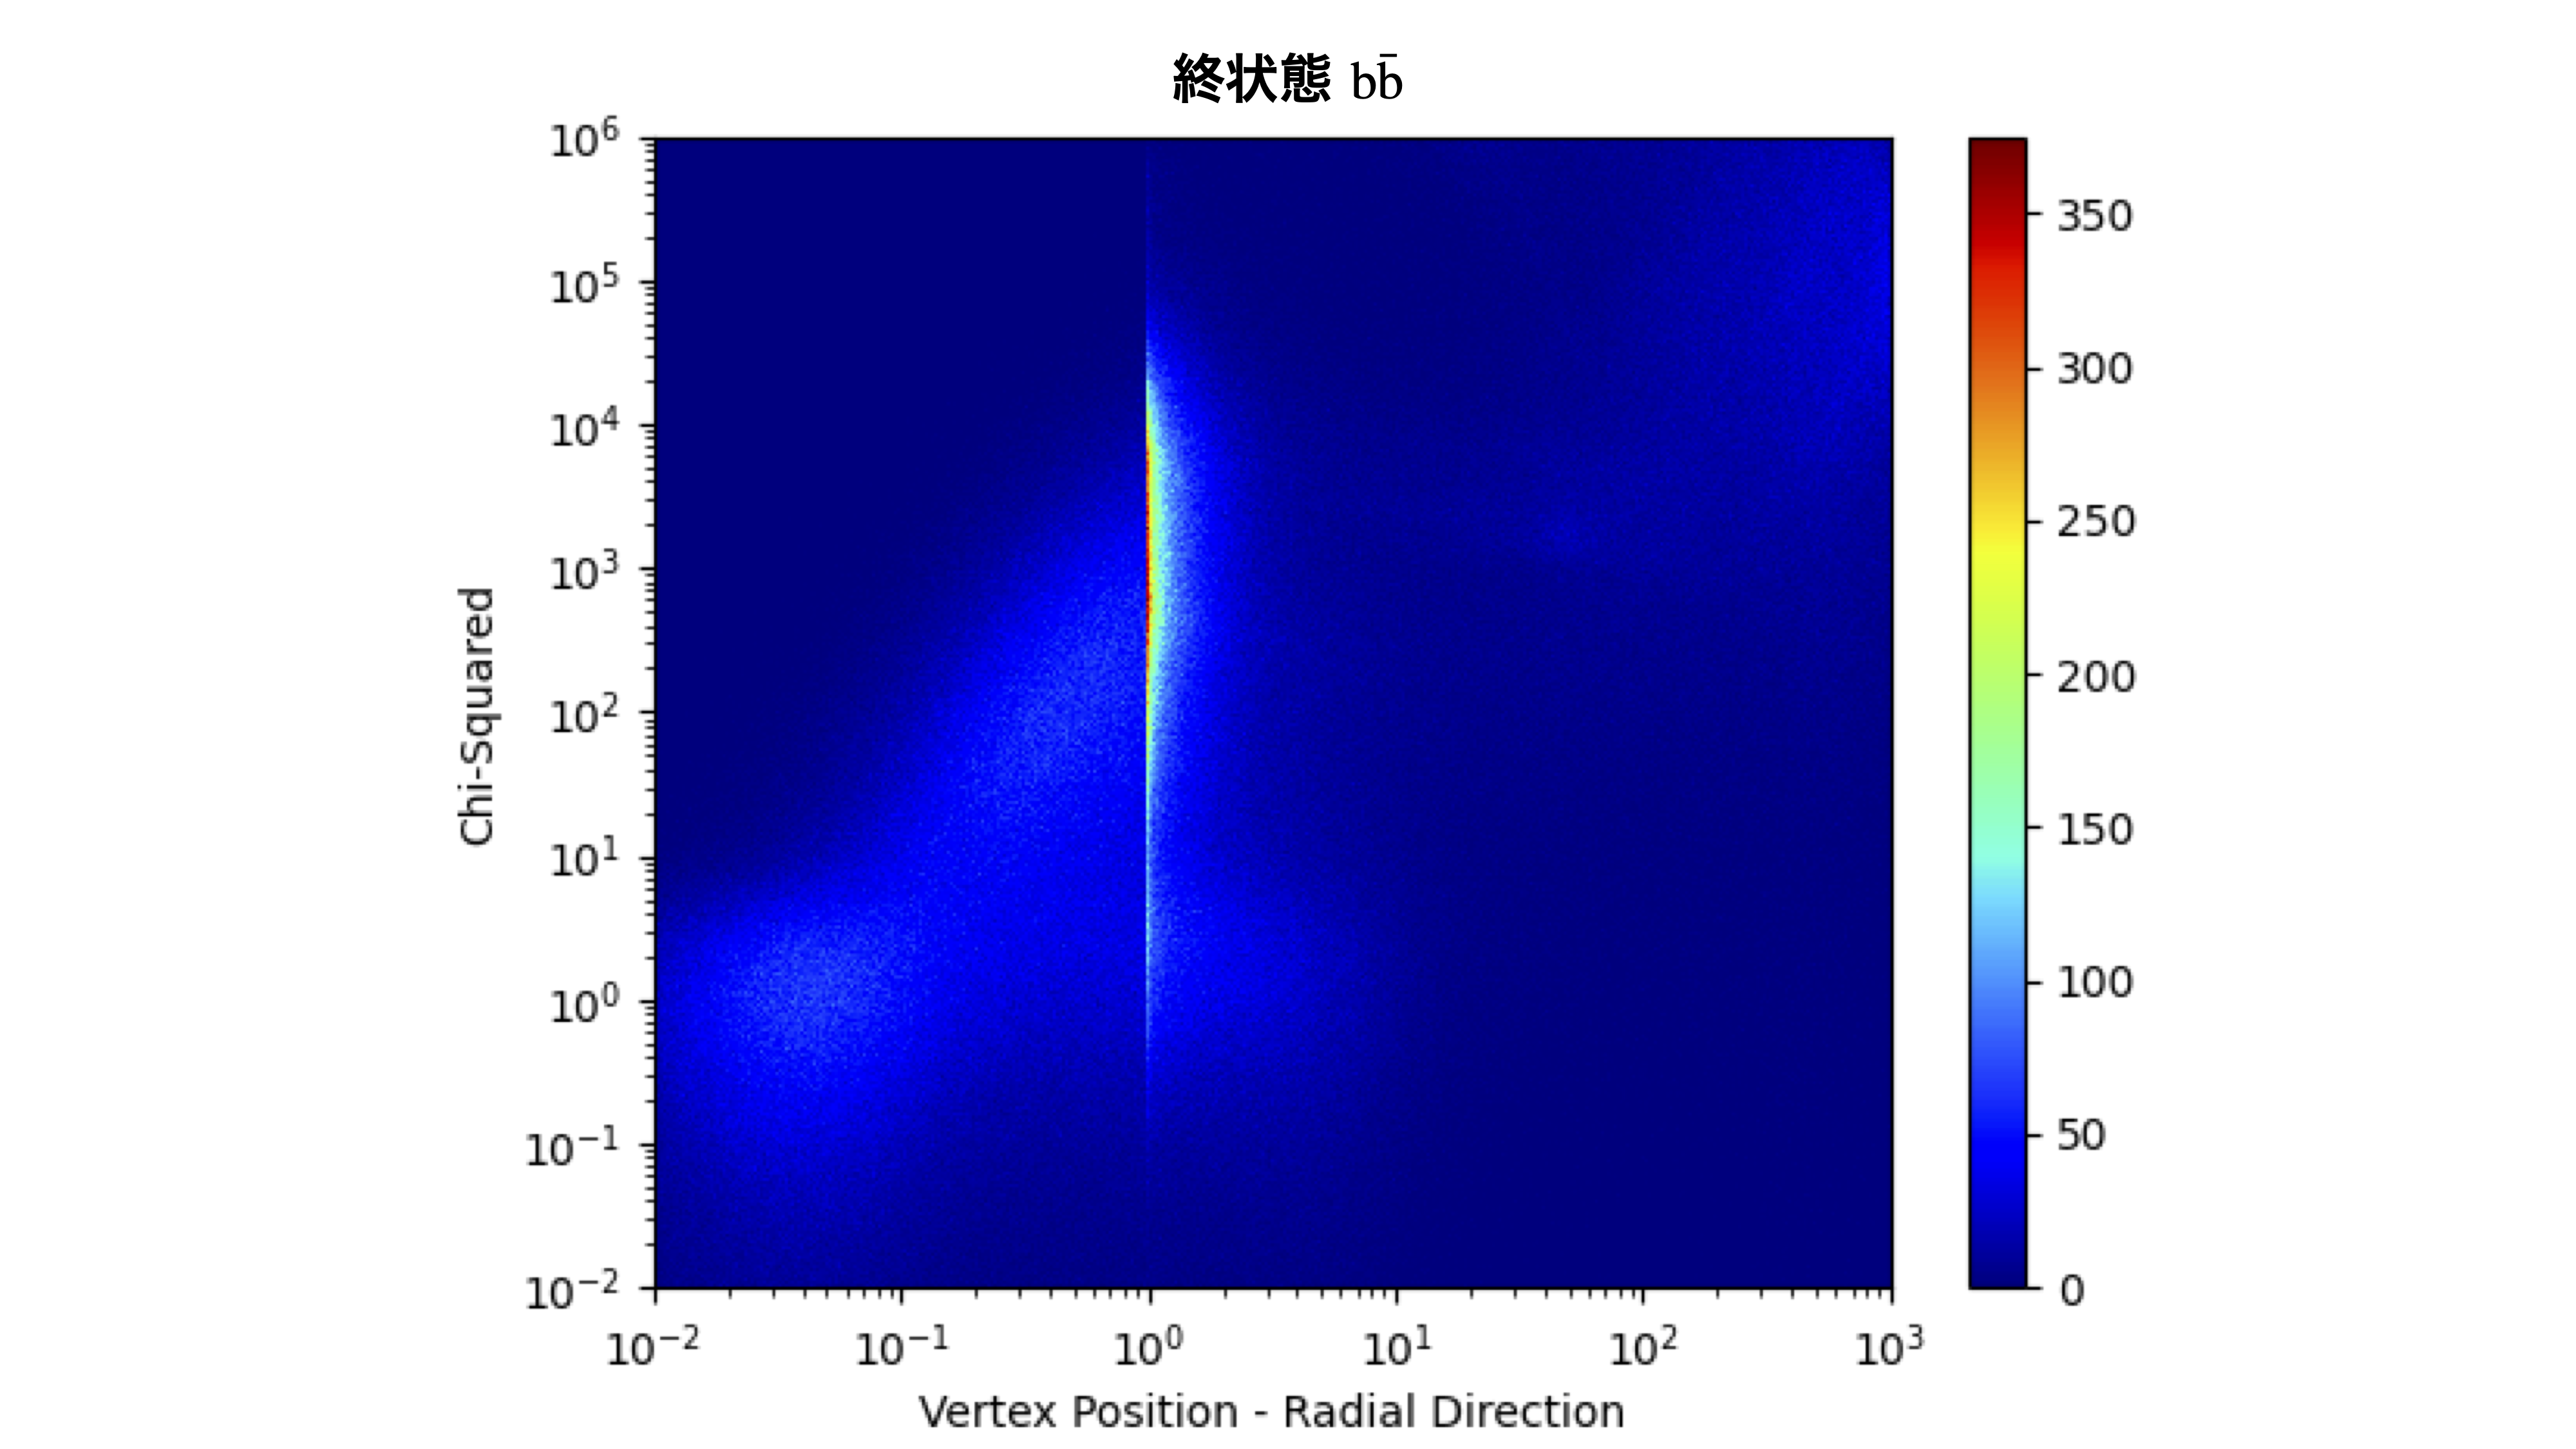
\includegraphics[width=1.0\textwidth, clip]{Figure/3Networks/3-1-2-4VertexPositionsvsChiSquare.png}
 \caption[LCFIPlusによって予想される崩壊点の位置と$\chi^2$値の相関]{LCFIPlusによって予想される崩壊点の位置と$\chi^2$値の相関。縦軸, 横軸はそれぞれログスケールの$\chi^2$値, ログスケールの衝突点からの距離である。カラースケールはカウントを示しており, $1\ \mathrm{mm}$付近で非常に大きな値になっていることがわかる。}
 \label{3-1-2-4VertexPositionsvsChiSquare}
\end{figure}

\newpage
%%%%%%%%%%%%%%%%%%%%%%%%%%%%%%%%%%%%%%%%%%%%%%%%%%%%%%%%%%%%%%%%%%%%%%%%%%%%%%%%%%%%%%%%%%%%%%%%%%%%%
\section{深層学習を用いた崩壊点検出の実現} \label{Net:forVertexFinderwithDL}

深層学習は分類問題や回帰問題を解けるが, 一方で基本的にはクラスタリングなど教師なし学習に対しては不向きである。
分類問題や回帰問題では訓練データから「パターン」を学び, データの持つ特徴量の空間内である種の境界を引く必要がある。
この「パターン」はあらゆるデータ内で分類可能な決まった性質を持っていなければならない。
例えば\ref{Net:Data:DataProperty}項では, 同一フレーバーのSecondary Vertexが主に二つあることを解説した。
この二つのSecondary Vertexは事象内では位置の違いによって区別できるが, あらゆる事象間で不変的に一番や二番といったラベル付けできる性質を持っていない。\footnote{実際には損失関数を最小にするような順序を与えることで分離することは可能であるが本研究においては様々なSecondary Vertexが存在する為不適である。}

崩壊点検出アルゴリズムの目的は同一フレーバー内の複数のSecondary Vertexを含む崩壊点を探索する事である。
このような問題は一般にクラスタリングを用いて解くことが多いが, 本研究で使用するデータは図\ref{3-1-1-2TracksandVertices}で示したように事象内に含まれる飛跡の本数や崩壊点の個数も異なっているという性質を持っている。
これはクラスター数やクラスターに含まれる要素数が常に変わってしまうということを意味しており, 崩壊点検出をクラスタリングで行うことは不適であると判断した。

以上を踏まえた上で私は次の二つのネットワークを用いた崩壊点検出を提案する。

\begin{enumerate}
 \item 飛跡対についてのネットワーク
 \begin{itemize}
  \item 用途 : 崩壊点のタネの探索
  \item 入力 : 事象内のあらゆる飛跡対 (二本の飛跡の全ての組み合わせ)
  \item 出力 : 飛跡対の属する崩壊点の種類・崩壊点の位置
 \end{itemize}
 \item 任意の数の飛跡についてのネットワーク
 \begin{itemize}
  \item 用途 : 崩壊点の生成
  \item 入力 : 崩壊点のタネ・事象内の全ての飛跡
  \item 出力 : 事象内のそれぞれの飛跡が崩壊点のタネに結合しているか否か
 \end{itemize}
\end{enumerate}

飛跡対についてのネットワークは崩壊点のタネとなる飛跡対を探索するネットワークである。
したがって, このネットワーク単体では崩壊点を形成することはできない。
そこで, 私は崩壊点の生成を行う, もう一つのネットワークを構築した。
崩壊点の生成を行うネットワークは二本以上の飛跡を取り扱う必要があるが, 三本, 四本, 五本の飛跡を取り扱えるネットワークをそれぞれ構築することはネットワークや組み合わせの数を考える上で適切ではない。
よって不定の数の飛跡を再帰的に処理するネットワーク構造として, リカレントニューラルネットワークを使用した。
任意の数の飛跡についてのネットワークは崩壊点のタネをリカレントニューラルネットワークの初期状態として, そこに飛跡を一本ずつ加え崩壊点の生成を行うネットワークである。
本研究は以上の二つのネットワークを用いることで崩壊点検出を実現した。
構造や学習についての, より詳細な個々のネットワークの解説は, 後の\ref{Net:PairModel}節や\ref{Net:VertexLSTM}節で述べる。

本研究のネットワークはTensorflow/Kerasフレームワークを用いて構築・学習を行なった。
また, 学習に際しては計算機として, 弊研究室サーバーの"NVIDIA TITAN RTX"や九州大学情報基盤研究開発センター研究用計算機システムの一般利用を使用した。
詳細なソフトウェア・ハードウェアの環境を表\ref{SoftwareHardwareEnvironments}に示す。

\begin{table}[htb]
 \centering
 \small
  \begin{tabular*}{0.75\textwidth}{@{\extracolsep{\fill}}l l}\hline
    ソフトウェア&\\\hline\hline
    Python & $3.6.8$\\
    Tensorflow & $2.1.0$\\
    Keras & $2.3.1$\\\hline
    ハードウェア &\\\hline\hline
    CPU& AMD EPYC 7402P 24-Core Processor 48個\\
    メモリ & $263694036\ \mathrm{kB}$\\
    GPU & NVIDIA Corporation TU102 [TITAN RTX] 2個\\\hline
  \end{tabular*}
  \caption{ソフトウェア・ハードウェアの環境}
  \label{SoftwareHardwareEnvironments}
\end{table}


%%%%%%%%%%%%%%%%%%%%%%%%%%%%%%%%%%%%%%%%%%%%%%%%%%%%%%%%%%%%%%%%%%%%%%%%%%%%%%%%%%%%%%%%%%%%%%%%%%%%%
\section{飛跡対についてのネットワーク} \label{Net:PairModel}

ここでは\ref{Net:forVertexFinderwithDL}節で紹介した二つのネットワークの内, 飛跡対についてのネットワークに関して述べる。
主にネットワークの構造に関しては\ref{Net:PM:StructureofPM}項で, 学習に関しては\ref{Net:PM:TrainingandStrategyofPM}項で解説する。
また, そのようにして構築, 訓練されたネットワーク単体についての性能と評価に関しては, \ref{Net:PM:PerformanceofPM}項で述べることとする。

飛跡対についてのネットワークは, 崩壊点のタネを探索するためのネットワークであり, 入力は二本の飛跡についての情報, 出力は飛跡対についての崩壊点の種類や位置である。
この崩壊点の種類を考える上で\ref{Net:Data:DataProperty}項で述べた, 終状態によって生じる崩壊点の種類の違いを考慮しなければならない。
例えば, 終状態$\rm b\bar{b}$の場合は$\rm b \to c$という崩壊過程を辿り, ボトム・フレーバーのSecondary Vertexとチャーム・フレーバーのTertiary Vertexが生じ, 終状態$\rm c\bar{c}$の場合はチャーム・フレーバーのSecondary Vertexのみが生じる。
また両方の終状態について, これら以外の崩壊点であるOthers\footnote{タウ粒子の崩壊やストレンジ ($\rm s$) ・フレーバーのハドロンの崩壊, 光子変換}を考える必要がある。
更に終状態$\rm b\bar{b}$の場合について, ボトム・フレーバーのSecondary Vertexからの飛跡とそこから生じたチャーム・フレーバーのTertiary Vertexからの飛跡を一本ずつ含んだ飛跡対を準崩壊点として定義する。 (図\ref{3-3-0-1SecondaryVertexBC}) 

以上より, 飛跡対についての崩壊点の種類は"非結合な飛跡対 (Not Connected, NC)", "Primary Vertex (PV)", "チャーム・フレーバーのSecondary Vertex (SVCC)", "ボトム・フレーバーのSecondary Vertex (SVBB)", "チャーム・フレーバーのTertiary Vertex (TVCC)", "終状態$\rm b\bar{b}$での準崩壊点 (SVBC)", "これら以外の崩壊点 (Others)"の計$7$つとなる。

\begin{figure}[htbp]
 \centering
 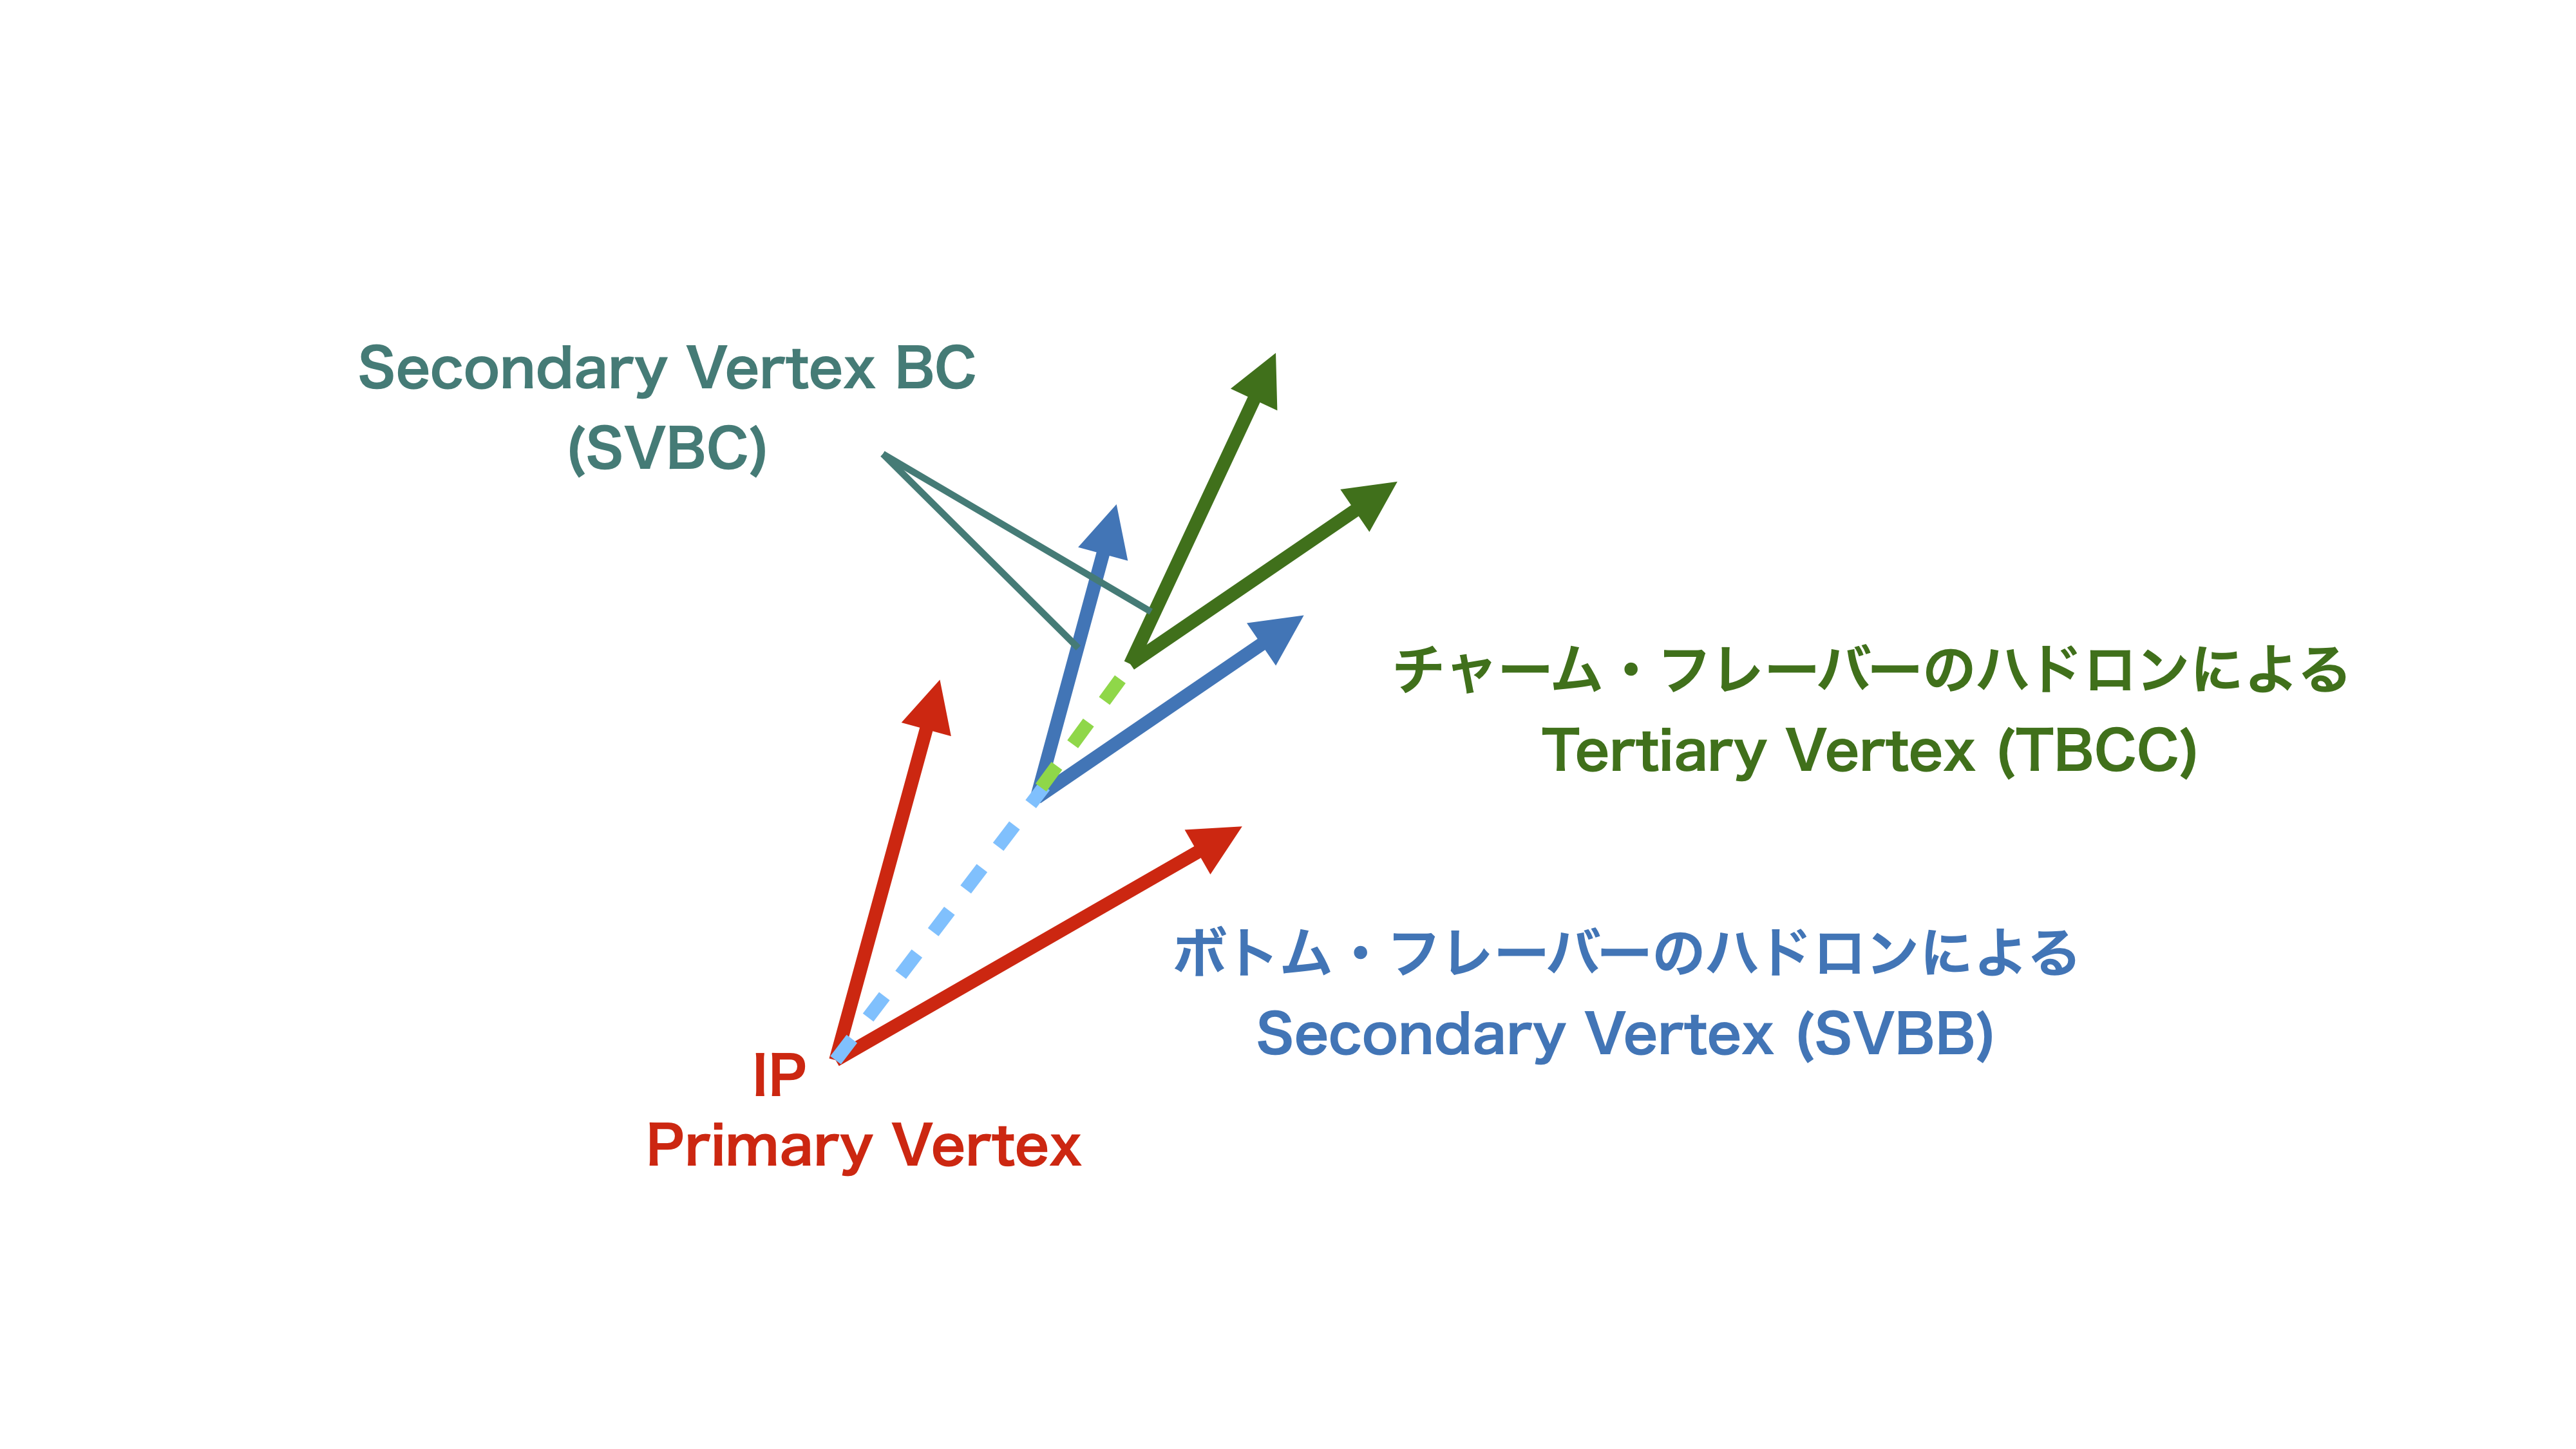
\includegraphics[trim = 200 150 200 150, width=0.9\textwidth, clip]{Figure/3Networks/3-3-0-1SecondaryVertexBC.png}
 \caption{終状態$\rm b\bar{b}$での崩壊点}
 \label{3-3-0-1SecondaryVertexBC}
\end{figure}

崩壊点の位置についての訓練データを作成するに当たって, 正解ラベルとして図\ref{3-1-2-3VertexPositions}のLCFIPlusのフィッティングで得られる計算値を用いた。
こちらは回帰によって値を再現する。


%%%%%%%%%%%%%%%%%%%%%%%%%%%%%%%%%%%%%%%%%%%%%%%%%%%%%%%%%%%%%%%%%%%%%%%%
\subsection{ネットワークの構造} \label{Net:PM:StructureofPM}

飛跡対についてのネットワークとして非常にシンプルなフィードフォーワード構造を使用した。
ネットワークの概略図を図\ref{3-3-1-1PairModel}に示す。

\begin{figure}[htbp]
 \centering
 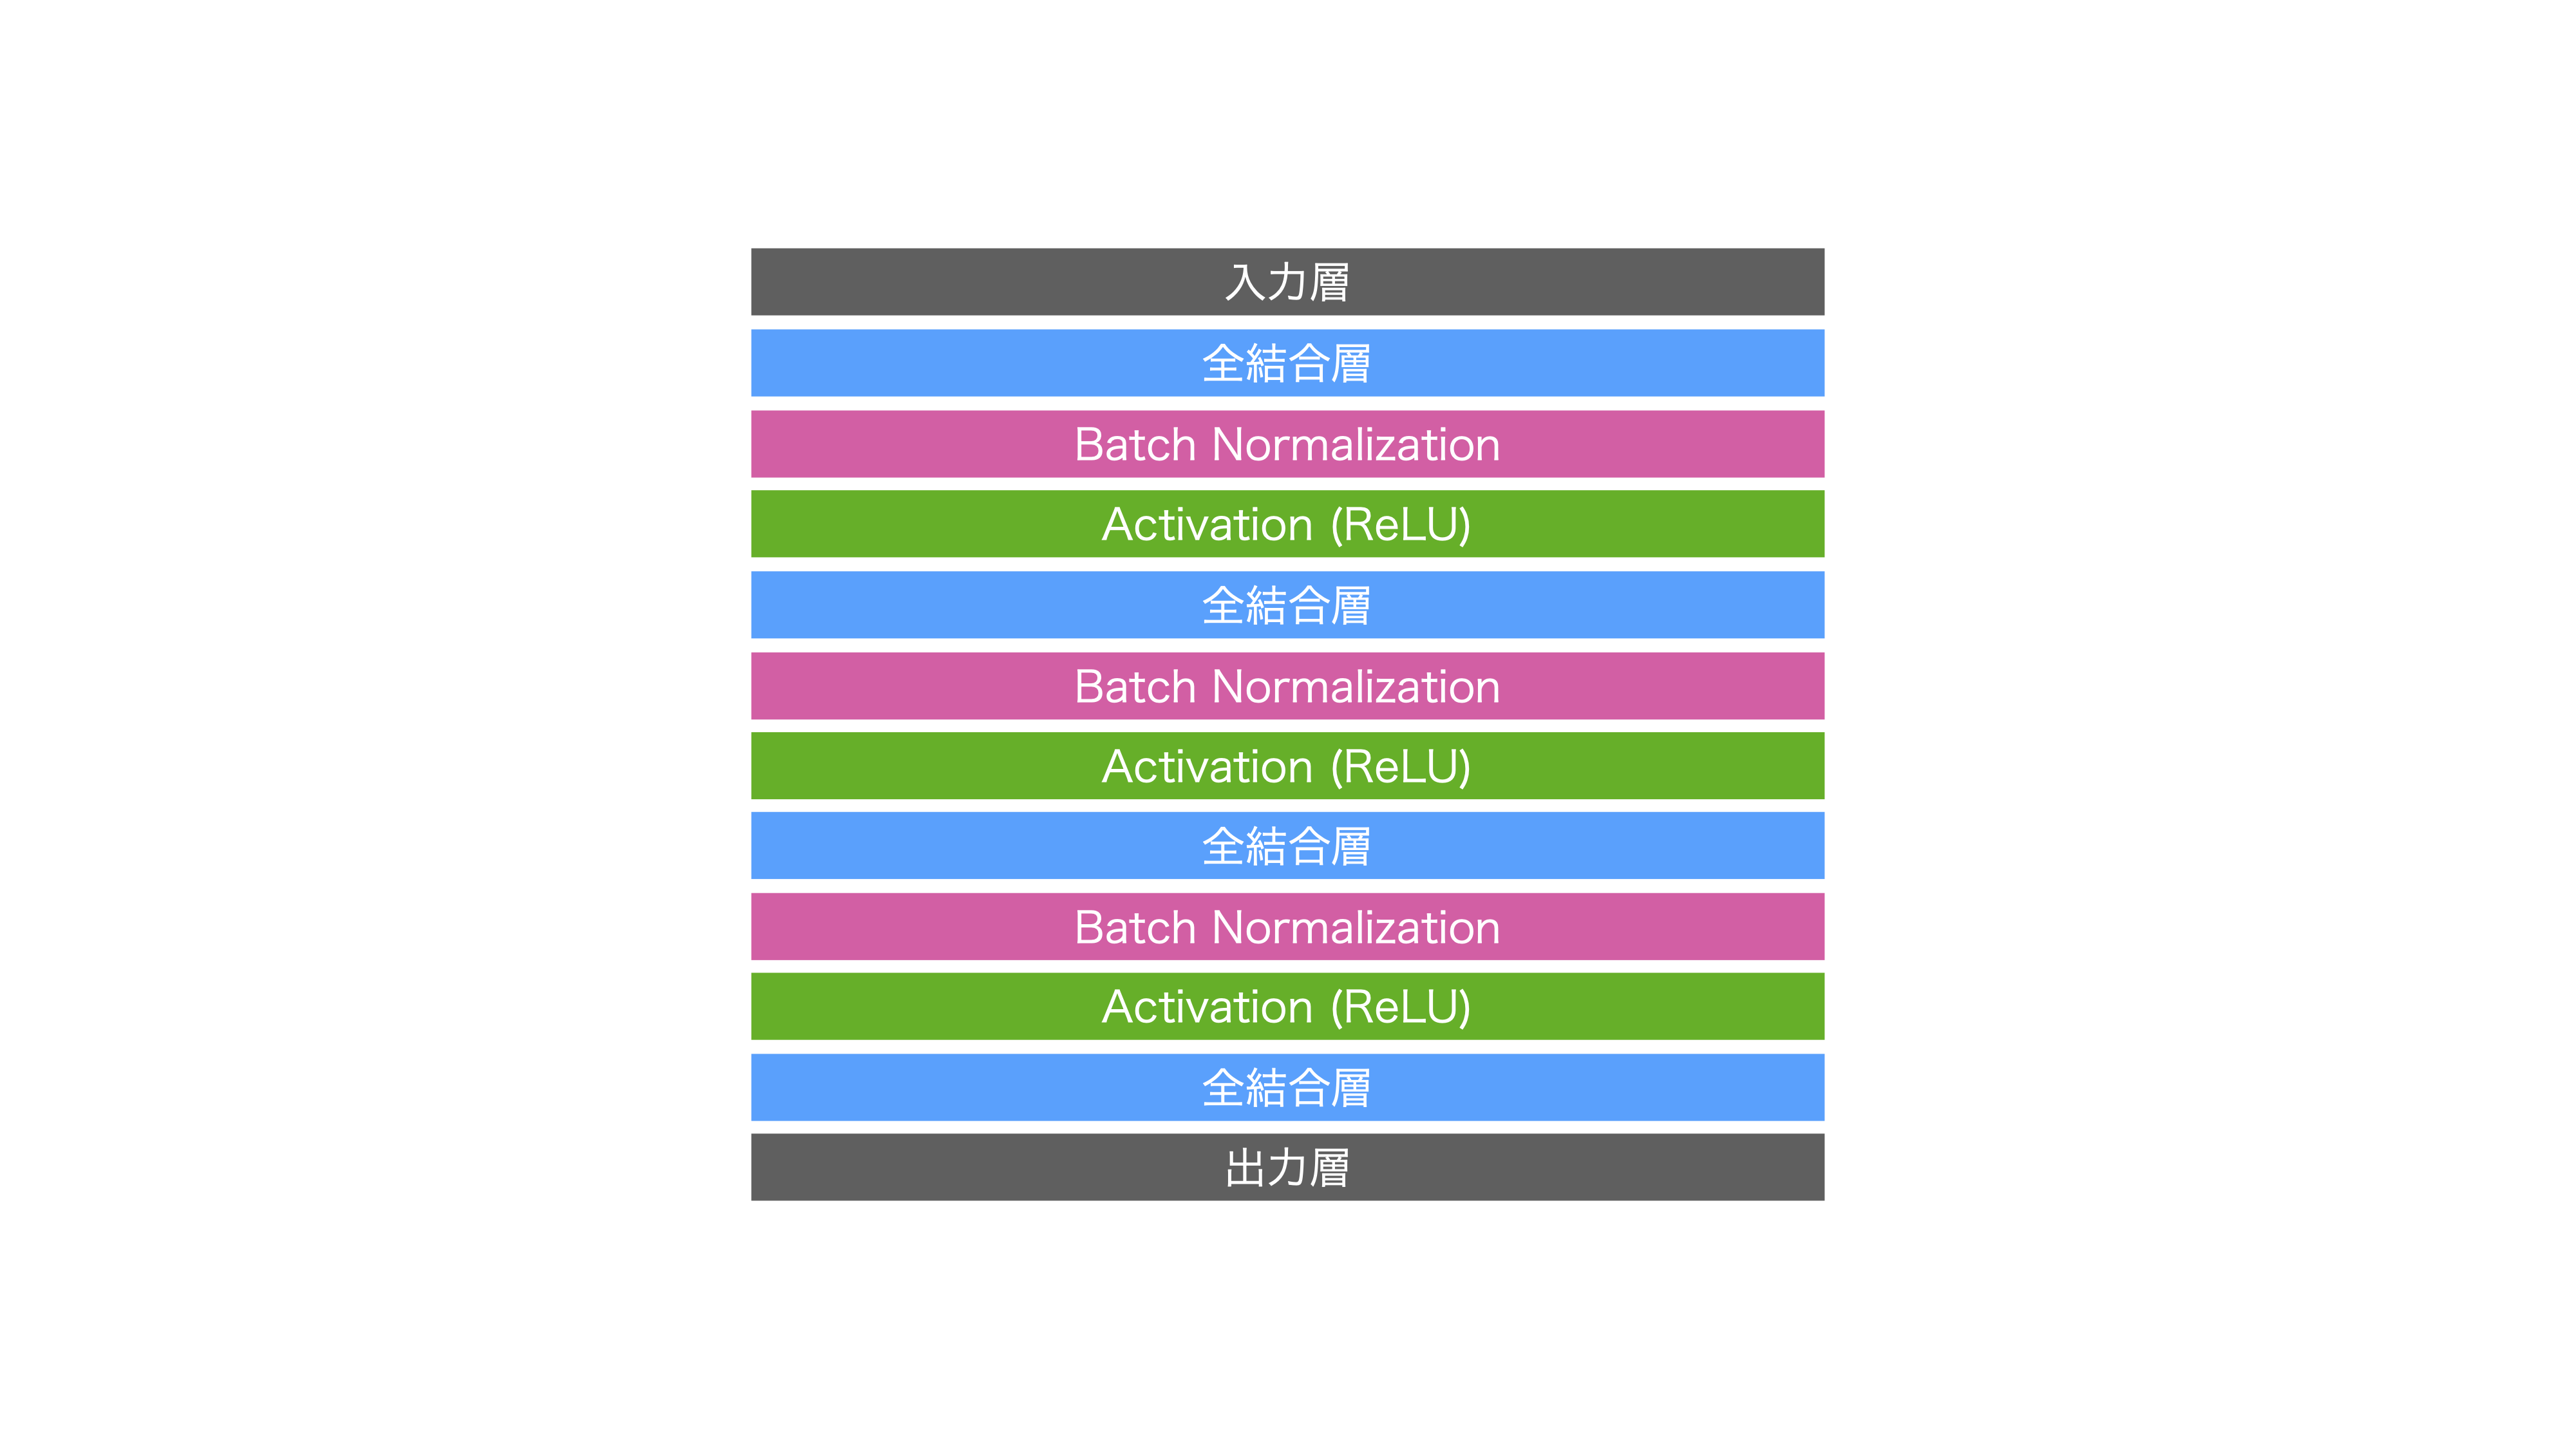
\includegraphics[trim = 200 50 200 50, width=0.9\textwidth, clip]{Figure/3Networks/3-3-1-1PairModel.png}
 \caption[飛跡対についてのネットワークの概略図]{飛跡対についてのネットワークの概略図。全結合層・Batch Normalization・活性化関数 (ReLU) を三回重ねている。その後, 分類問題の為の全結合層と回帰問題の為の全結合層の二つに分離させ, それぞれで出力を行う。}
 \label{3-3-1-1PairModel}
\end{figure}

前述したように出力は, 7クラス分類と回帰1つである。
出力の直前の全結合層で分類問題と回帰問題に分離させた。
また, 過学習 (Over fitting) を避ける為, Batch Normalization\cite{BatchNormalizationpaper}を全結合層の後に配置した。
過学習とは, ネットワークが過度に訓練データに適合してしまい, 検証データやテストデータへの汎化性能が悪化してしまう, 教師あり学習の問題の一つである。
また勾配消失への対策として, 活性化関数は全てReLU関数を使用した。


%%%%%%%%%%%%%%%%%%%%%%%%%%%%%%%%%%%%%%%%%%%%%%%%%%%%%%%%%%%%%%%%%%%%%%%%
\subsection{ネットワークの学習と戦略} \label{Net:PM:TrainingandStrategyofPM}

訓練データは事象中の全ての飛跡対の組み合わせを考える。
よって入力変数は飛跡二本分であるので合計$44$個である。
ここで次の二つの事柄に注意しなくてはならない。

\begin{itemize}
 \item 分類クラスは二つの終状態$\rm b\bar{b}$と$\rm c\bar{c}$を足し合わせたものである
 \item 分類クラスのデータ数の比がNCやPVが支配的な不均衡データ (Imbalanced Data) となる
\end{itemize}

各終状態での分類クラスのデータ数の比を図\ref{3-3-2-1ImbalancedData}に示す。

\begin{figure}[htbp]
 \centering
 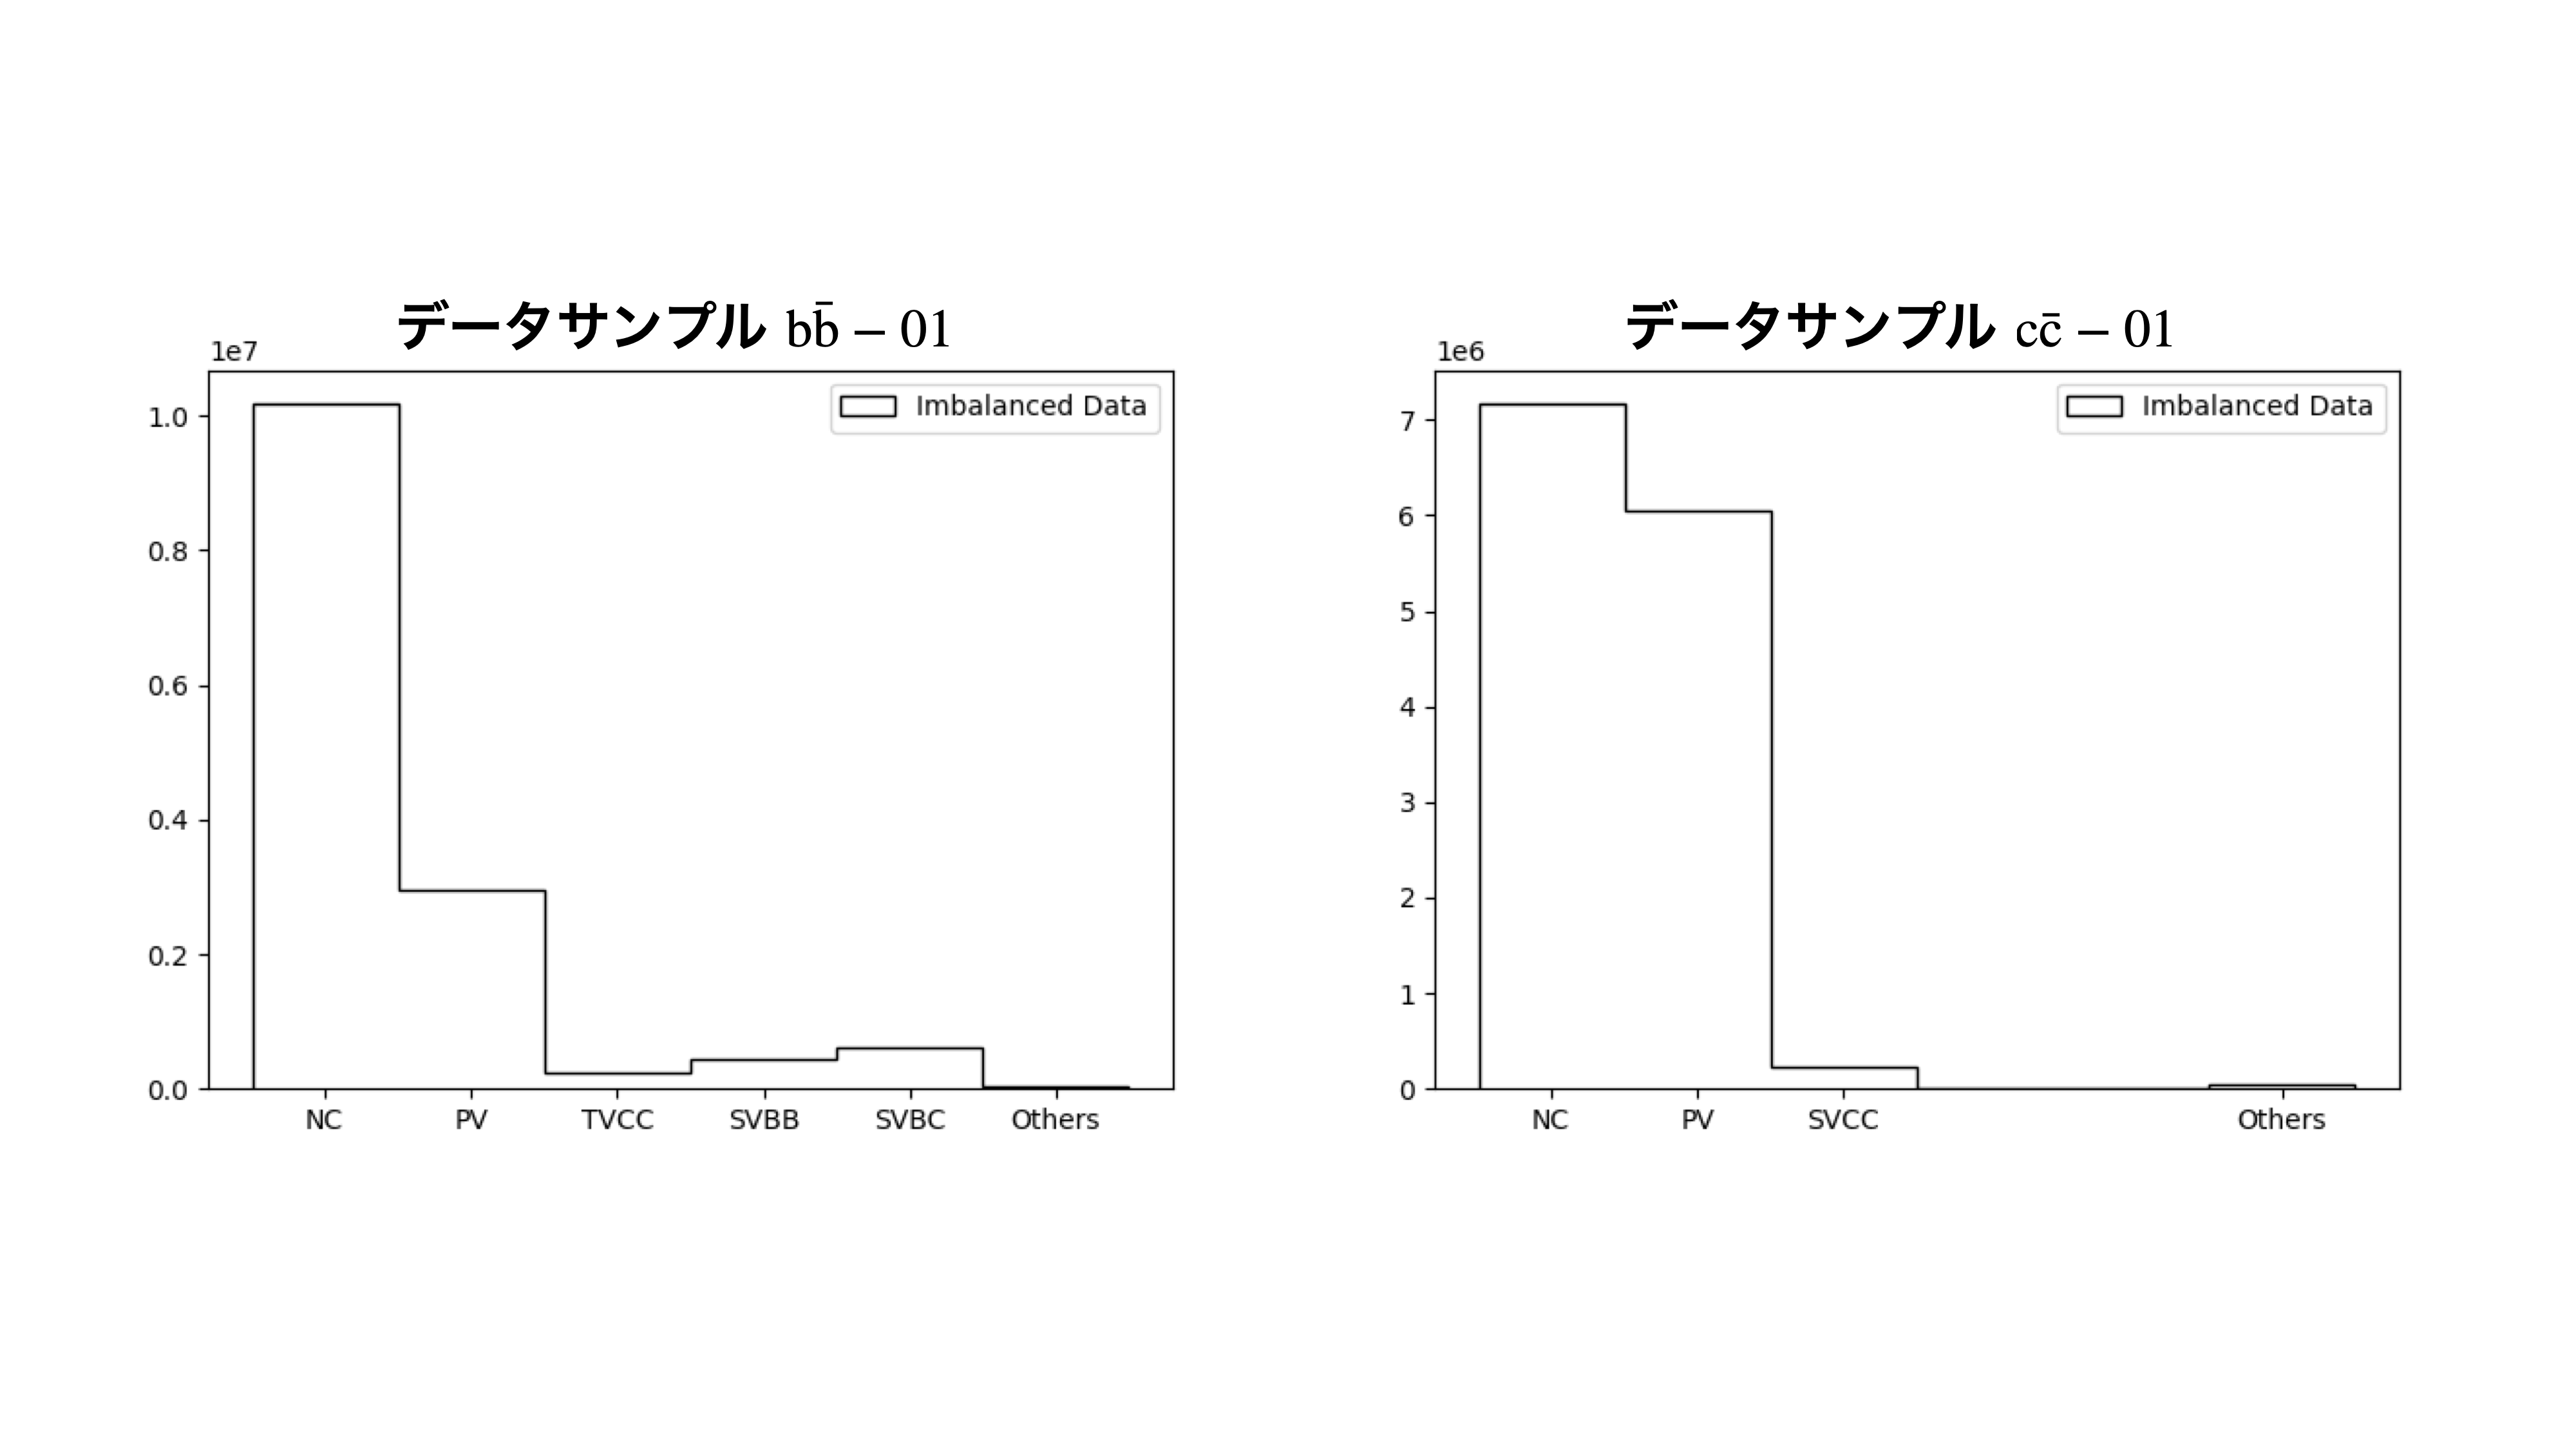
\includegraphics[trim = 100 200 100 150, width=0.9\textwidth, clip]{Figure/3Networks/3-3-2-1ImbalancedData.png}
 \caption[各終状態での分類クラスのデータ数の比]{各終状態での分類クラスのデータ数の比。図左が終状態$\rm b\bar{b}$, 図右が終状態$\rm c\bar{c}$である。終状態$\rm c\bar{c}$ではSVCC以外のSVが基本的に存在しない為, 終状態$\rm b\bar{b}$と比較してPVの比率が多くなっている。}
 \label{3-3-2-1ImbalancedData}
\end{figure}

このような不均衡データについては, 少数クラスのデータをかさ増しするオーバーサンプリング, 多数クラスのデータを間引くアンダーサンプリング, 損失関数のコストに重みをつけるコスト考慮型学習の主に三つの対応策が存在する。
オーバーサンプリングやアンダーサンプリングは過学習や情報の欠損などの問題を抱えているため, 本研究では基本的にコスト考慮型学習を用いる。
ただし, 二つの終状態のデータを単純に足し合わせた場合, 共通する分類クラスであるNCやPVがより顕著になり, 他クラスの学習が不十分になると考えられる。
このためNCやPVに関しては各終状態毎に半分にランダムサンプリングした後, 終状態$\rm b\bar{b}$と$\rm c\bar{c}$を足し合わせた。
最終的な訓練データでの分類クラスのデータ数の比を図\ref{3-3-2-2ImbalancedData}に示す。

\begin{figure}[htbp]
 \centering
 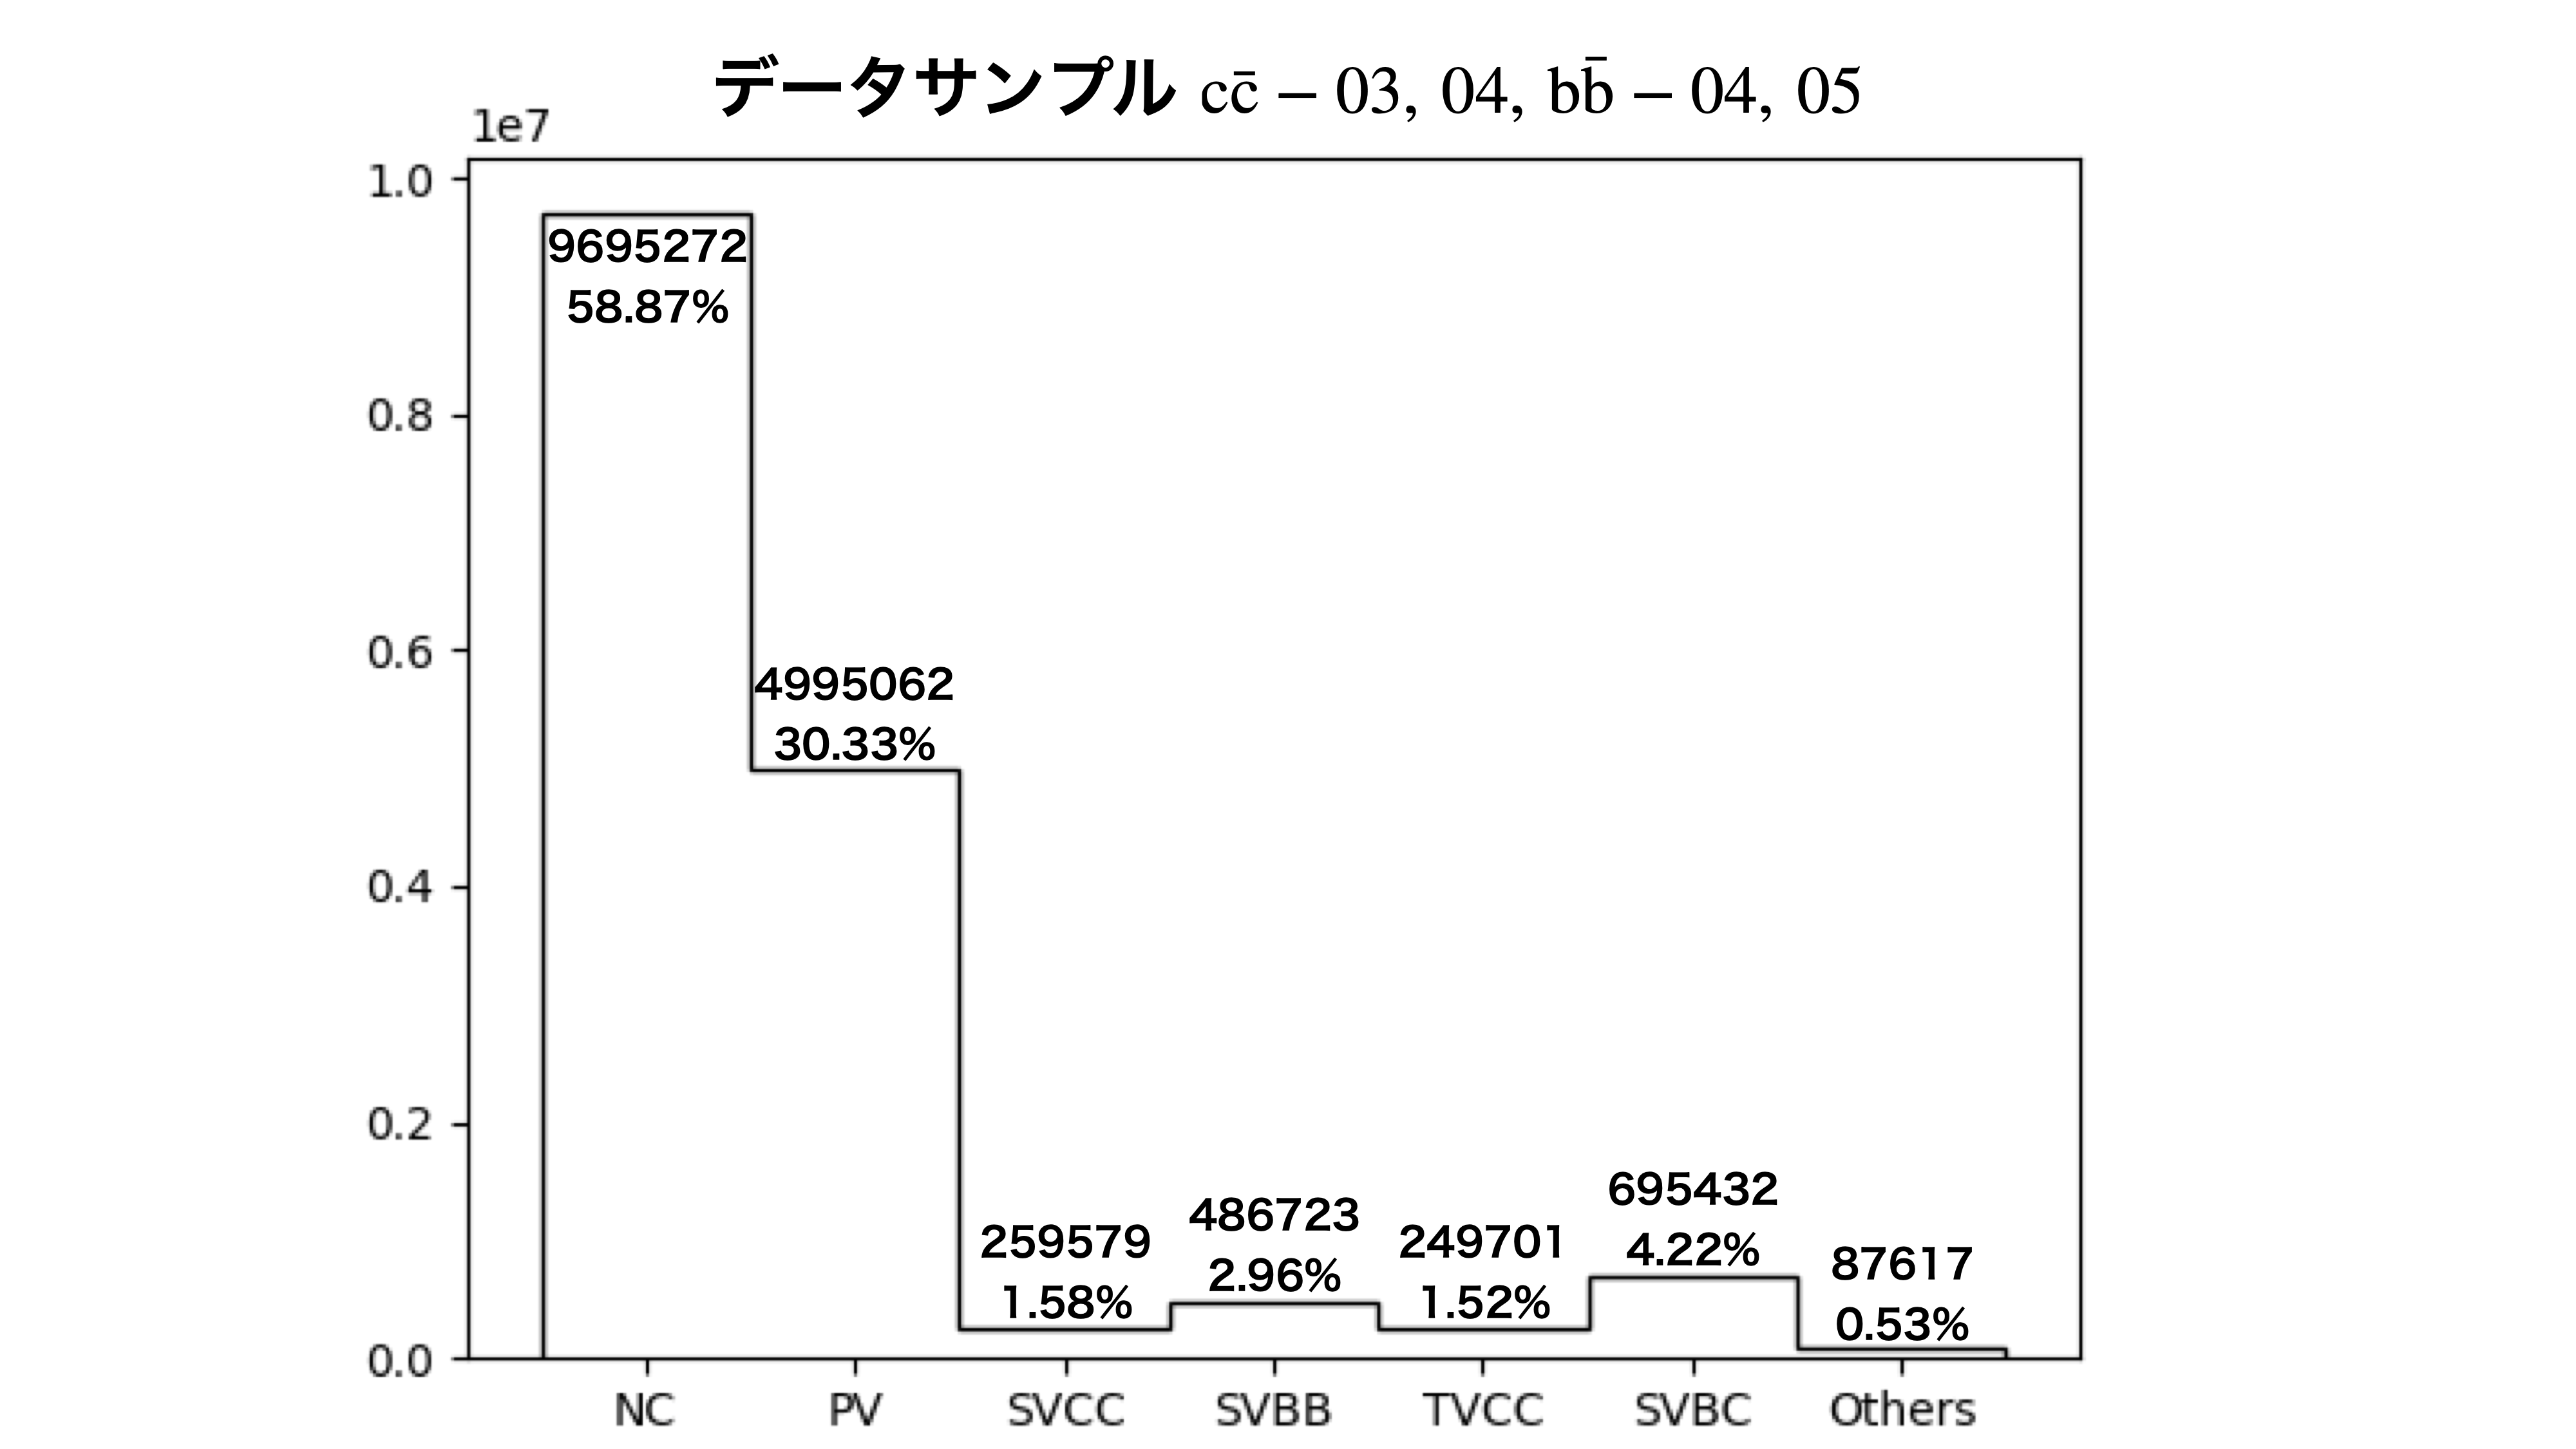
\includegraphics[width=1.0\textwidth]{Figure/3Networks/3-3-2-2ImbalancedData.png}
 \caption[訓練データでの分類クラスのデータ数の比]{訓練データでの分類クラスのデータ数の比。実際に使用する訓練データではNCとPVのカテゴリで全体の$9$割程度となっており, 非常に不均衡なデータとなっている。}
 \label{3-3-2-2ImbalancedData}
\end{figure}

損失関数$L$は分類問題である崩壊点の種類に関しての損失関数$L_{\rm CE}$と回帰問題である崩壊点の位置に関しての損失関数$L_{\rm LMSE}$の二つの合計となる。

本研究では, コスト考慮型学習として損失関数$L_{\rm CE}$の各クラスへの重みは, 分類クラスのデータ数の比の逆数を使用し不均衡データへ対策を行なった。
ここでは最も数の少ないOthersの重みを$1$としている。
\begin{equation}
 \begin{split}
 L_{\rm CE} = & - 0.0090\  t_{\rm NC} \log{(y_{\rm NC})} - 0.0175\  t_{\rm PV} \log{(y_{\rm PV})} \\
       & - 0.3375\  t_{\rm SVCC} \log{(y_{\rm SVCC})} - 0.1800\  t_{\rm SVBB} \log{(y_{\rm SVBB})}\\
       & - 0.3509\  t_{\rm TVCC} \log{(y_{\rm TVCC})} - 0.1260\  t_{\rm SVBC} \log{(y_{\rm SVBC})}\\
       & - 1.0\  t_{\rm Others} \log{(y_{\rm Others})}\\
 \end{split}
\end{equation}
ここで, $t_{\rm NC},\ t_{\rm PV},\ t_{\rm SVCC},\ t_{\rm SVBB},\ t_{\rm TVCC},\ t_{\rm SVBC},\ t_{\rm Others}$はそれぞれの分類クラスについての正解ラベルである。
また, $y_{\rm NC},\ y_{\rm PV},\ y_{\rm SVCC},\ y_{\rm SVBB},\ y_{\rm TVCC},\ y_{\rm SVBC},\ y_{\rm Others}$はそれぞれの分類クラスについてネットワークで予想された確率である。

崩壊点の位置についての損失関数$L_{\rm LMSE}$として平均二乗誤差を使用した。
ただし, 図\ref{3-1-2-3VertexPositions}からも分かるように, 崩壊点の位置は非常に広い範囲に分布しているため, 出力や正解ラベルの自然対数を使用し
\begin{equation}
 \begin{split}
 L_{\rm LMSE} = (\ln{(t_{\rm Position}+1)} - \ln{(y_{\rm Position}+1)})^2
 \end{split}
\end{equation}
とした。
ここで, $t_{\rm Position},\ y_{\rm Position}$はそれぞれLCFIPlusのフィッターで予想された崩壊点の位置, ネットワークで予想された崩壊点の位置である。

以上より, 飛跡対についてのネットワークの損失関数$L$は
\begin{equation}
 \begin{split}
 L & = w_{\rm vertex} L_{\rm CE} + w_{\rm position} L_{\rm LMSE}
 \end{split}
\end{equation}
となる。
ここで, $w_{\rm vertex},\ w_{\rm position}$は各損失関数$L_{\rm CE},\ L_{\rm LMSE}$への重みである。

本ネットワークでは崩壊点の位置を学習した後に崩壊点の種類の分類を行なった。
これは崩壊点の位置, あるいはそのような情報を抽出できるネットワークのパラメータを利用して, 崩壊点の種類の分類を行なって欲しいという狙いからである。
これは転移学習 (Transfer Learning, TL) やファインチューニングという手法\footnote{これらの手法ではあらかじめ学習済みのネットワークを別の問題解決に活用するテクニックである}に似た発想であるが, 今回はこれら二つの手法とは異なり, ネットワークの重みは全て再学習に使用している。
学習は以下の手順で行う。

\begin{enumerate}
 \item $(w_{\rm vertex},\ w_{\rm position})=(0.1,\ 0.9)$, $1000\ \mathrm{epoch}$, 学習率${\rm LR}=0.001$
 \item $(w_{\rm vertex},\ w_{\rm position})=(0.9,\ 0.1)$, $1500\ \mathrm{epoch}$, 学習率${\rm LR}=0.001$
 \item $(w_{\rm vertex},\ w_{\rm position})=(0.95,\ 0.05)$, $500\ \mathrm{epoch}$, 学習率${\rm LR}=0.0001$
\end{enumerate}

また, 重み更新の最適化手法としてSGDを用いた。
これは, Adamなどでは収束が早すぎ, 過学習になる恐れがあったためである。
学習には$13175508$サンプル, 検証には$3293878$サンプルのデータを使用した。
ネットワークの学習可能な重みのパラメータ数を表\ref{ParametersforPairModel}に示す。

\begin{table}[htb]
 \centering
 \small
 \scalebox{0.8}{
  \begin{tabular*}{1.2\textwidth}{@{\extracolsep{\fill}}l c c l}\hline
    層の名称 & 出力の形状 & パラメータ数 & 接続先\\\hline\hline
    Pair Input & (None, 44) & 0 & \\\hline\hline
    Dense 1 & (None, 256) & 11520 & Pair Input\\\hline
    Batch Normalization 1 & (None, 256) & 1024 & Dense 1\\\hline
    Activation ReLU 1 & (None, 256) & 0 & Batch Normalization 1\\\hline
    Dense 2 & (None, 256) & 65792 & Activation ReLU 1\\\hline
    Batch Normalization 2 & (None, 256) & 1024 & Dense 2\\\hline
    Activation ReLU 2 & (None, 256) & 0 & Batch Normalization 2\\\hline
    Dense 3 & (None, 256) & 65792 & Activation ReLU 2\\\hline
    Batch Normalization 3 & (None, 256) & 1024 & Dense 3\\\hline
    Activation ReLU 3 & (None, 256) & 0 & Batch Normalization 3\\\hline\hline
    Vertex Dense & (None, 7) & 1799 & Activation ReLU 3\\\hline
    Vertex Output & (None, 7) & 0 & Vertex Dense\\\hline\hline
    Position Output & (None, 1) & 257 & Activation ReLU 3\\\hline\hline
  \end{tabular*}
  }
  \caption{飛跡対についてのネットワークにおける訓練可能なパラメータ}
  \label{ParametersforPairModel}
\end{table}


%%%%%%%%%%%%%%%%%%%%%%%%%%%%%%%%%%%%%%%%%%%%%%%%%%%%%%%%%%%%%%%%%%%%%%%%
\subsection{ネットワークの評価} \label{Net:PM:PerformanceofPM}

ネットワークの評価は1. ネットワーク間の比較, 2. ネットワーク内の理解の二つの観点によって行う。
本ネットワークでは, 1. ネットワーク間の比較については入力変数やネットワーク構造の異なる幾つかのネットワークのモデルについて比較を行う。
2. ネットワーク内の理解についてはt分布型確率的近傍埋め込み法(t-Distributed Stochastic Neighbor Embedding, t-SNE\cite{t-SNEpaper})を用いた次元削減によって, ネットワークによる情報の抽出や各クラスの分離について議論する。\\

1. ネットワーク間の比較\\

深層学習を取り扱う上で気を付けなければならない問題として, ネットワークの怠け(Lazy)が存在する。
ネットワークの怠けとは, ある入力変数について, 特定の要素にのみ注目する, あるいは特定の要素を無視してしまうという問題である。
飛跡対についてのネットワークでは, 深層学習が取り扱いづらい共分散を入力している。
ここではネットワークが共分散をどの程度取り扱えているかを評価するため, 共分散を含んだ入力変数を用いたモデルAと含んでいないモデルBを構築し比較を行なった。
ここでネットワークの構造として, 図\ref{3-3-1-1PairModel}を使用し, そのようなネットワークの構造をネットワーク$1$と呼ぶことにする。

また, \ref{Net:Data:TrackInformationandPreprocessing}節でも述べたように本研究における崩壊点の種類の分離において, 崩壊点の位置の再構成は必須である。
したがって, そのような崩壊点の位置についての情報を再構成し, 適切に処理出来ているかを把握するため, 本来回帰問題の正解ラベルとして用いているLCFIPlusによって予想された崩壊点の位置についての情報を出力層の直前で入力するネットワーク2を構築した。
更に, ネットワーク自体が予想した崩壊点の位置を明示的に入力に使用したネットワーク3の構築を行った。
これらネットワーク2, ネットワーク3を使用したモデルをそれぞれモデルC, モデルDとし前述のモデルA, モデルBとの比較を行なった。
それぞれのモデルの詳細を表\ref{EvalationModels}にまとめる。

\begin{figure}[htbp]
 \centering
  %\begin{tabular}{cccc}
  \begin{minipage}{1.0\textwidth}
  \centering
   \begin{minipage}{0.48\textwidth}
    \centering
    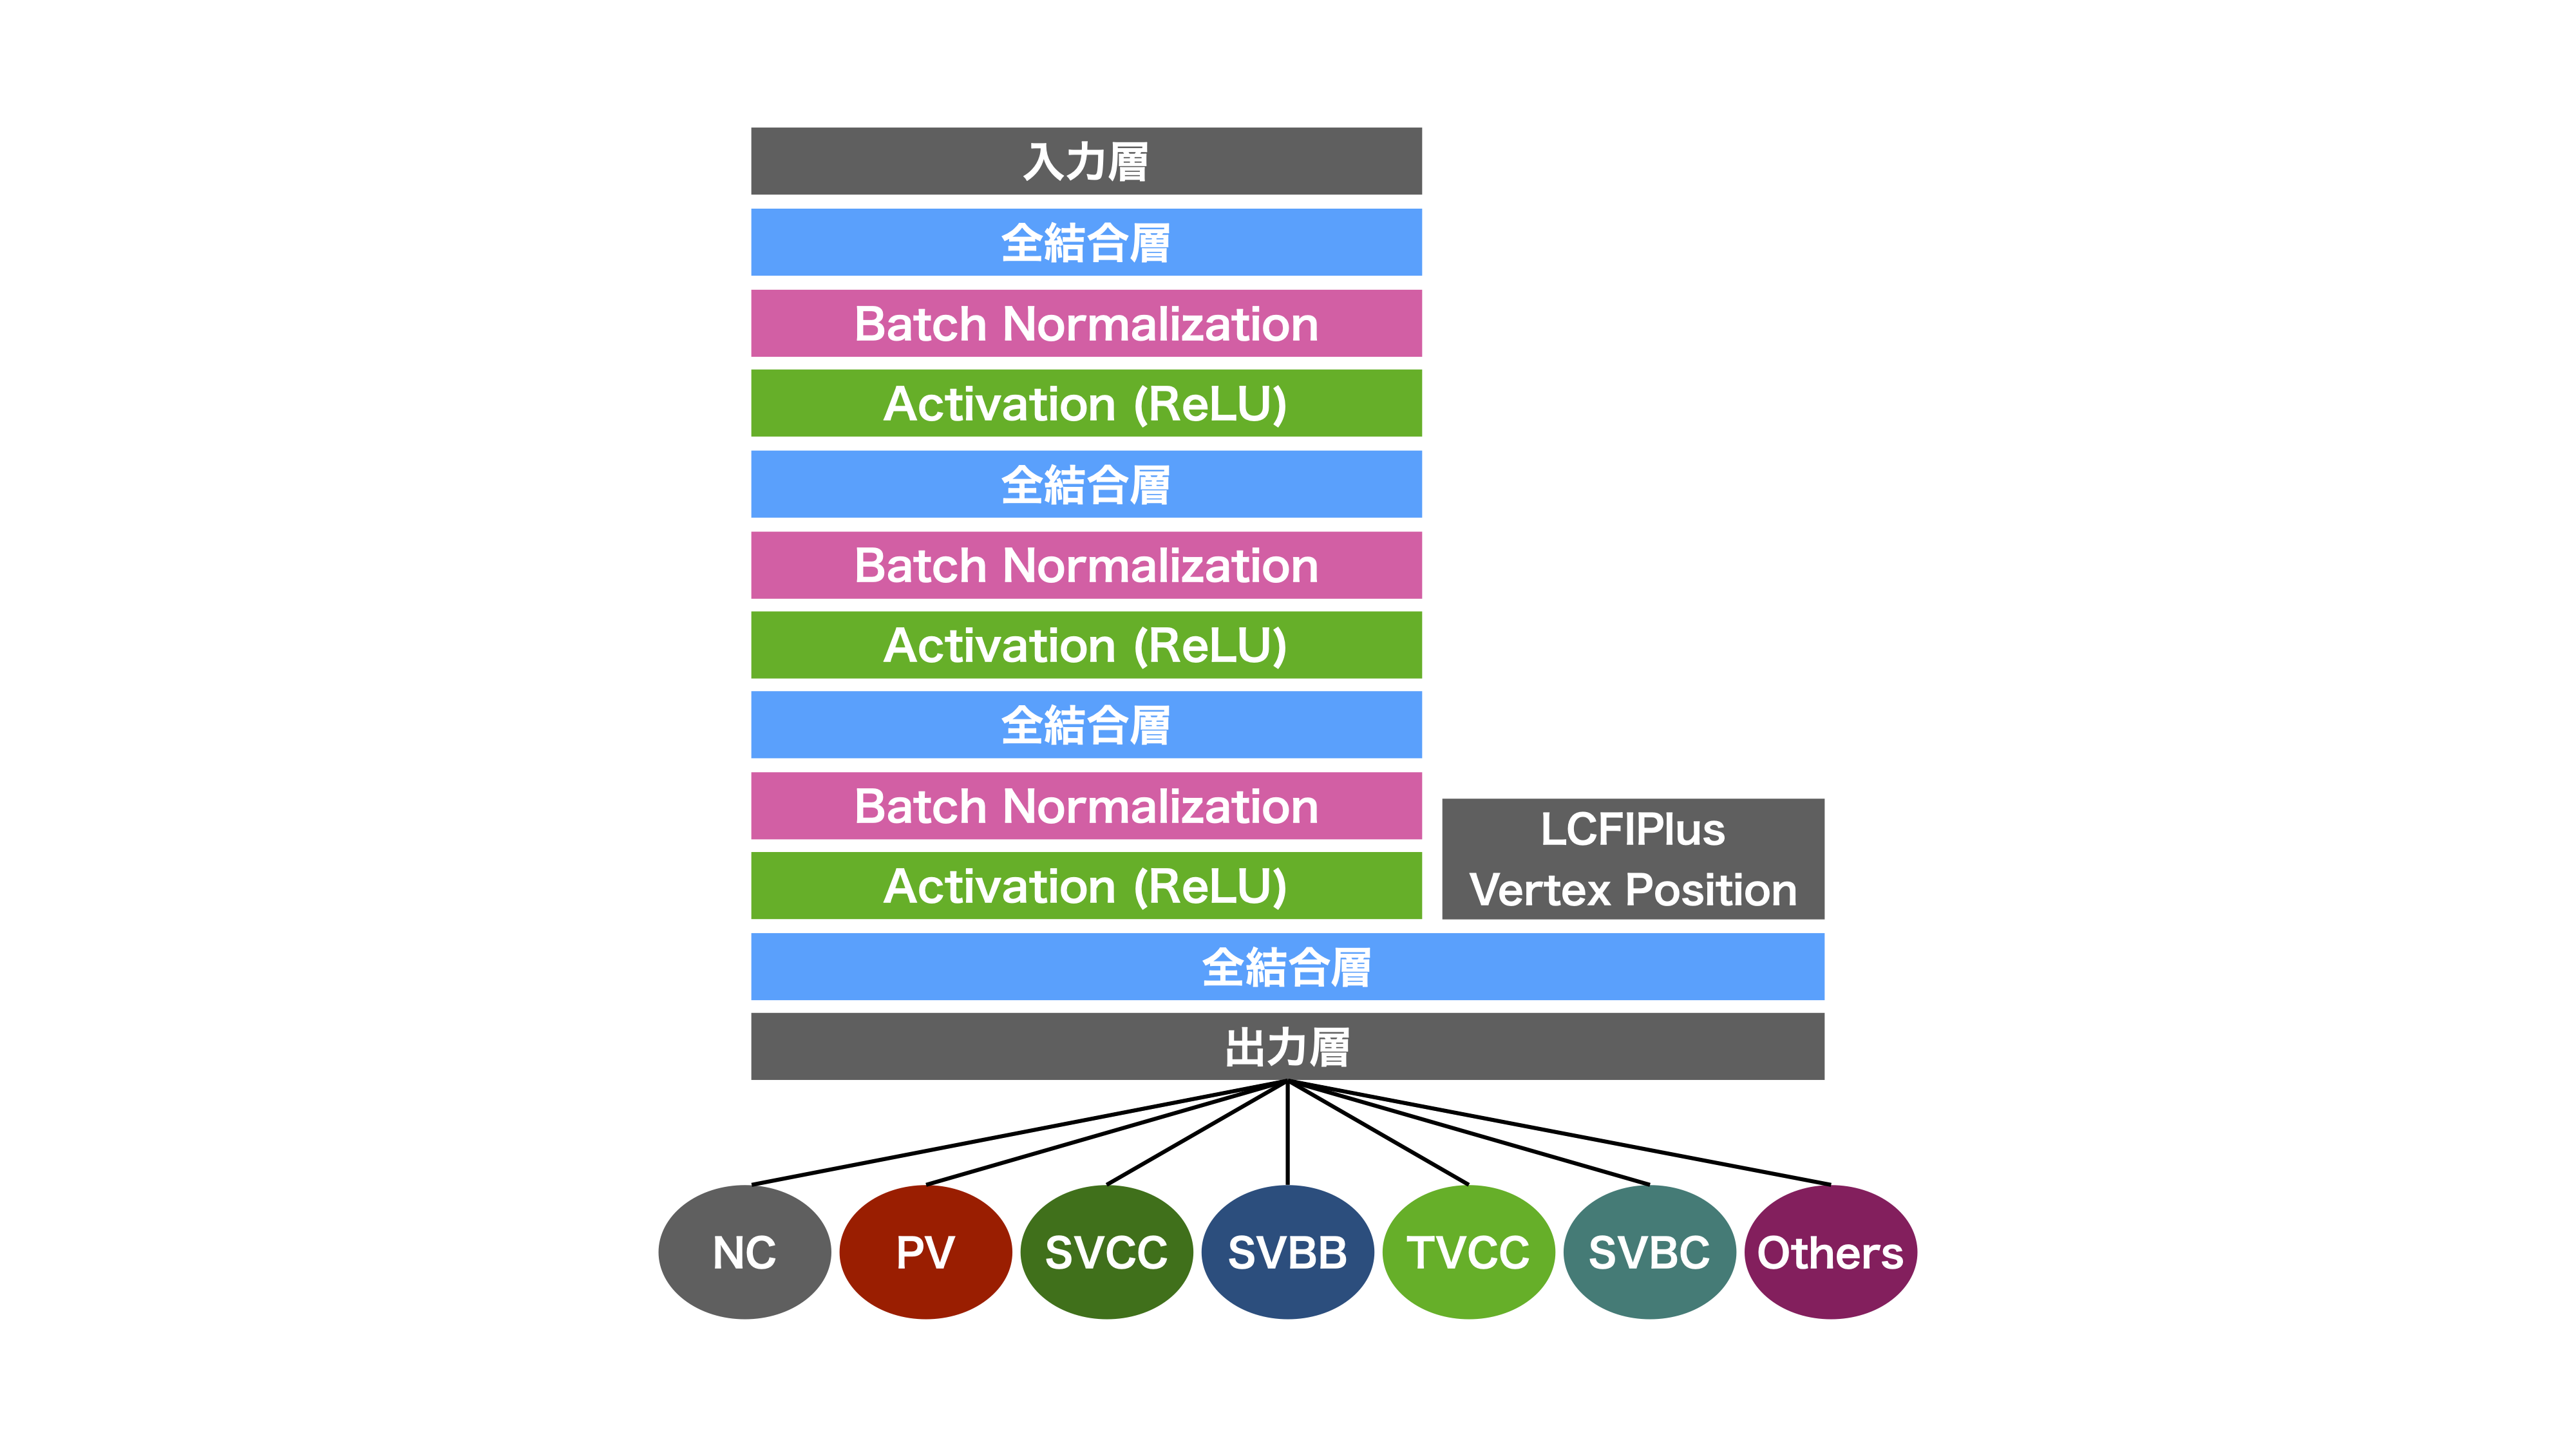
\includegraphics[trim = 200 0 200 0, width=1.0\textwidth, clip]{Figure/3Networks/3-3-3-1PairNetworkA.png}
    \subcaption{ネットワーク2}
    \label{3-3-3-1PairNetworkA}
   \end{minipage}
   \begin{minipage}{0.48\textwidth}
   \centering
    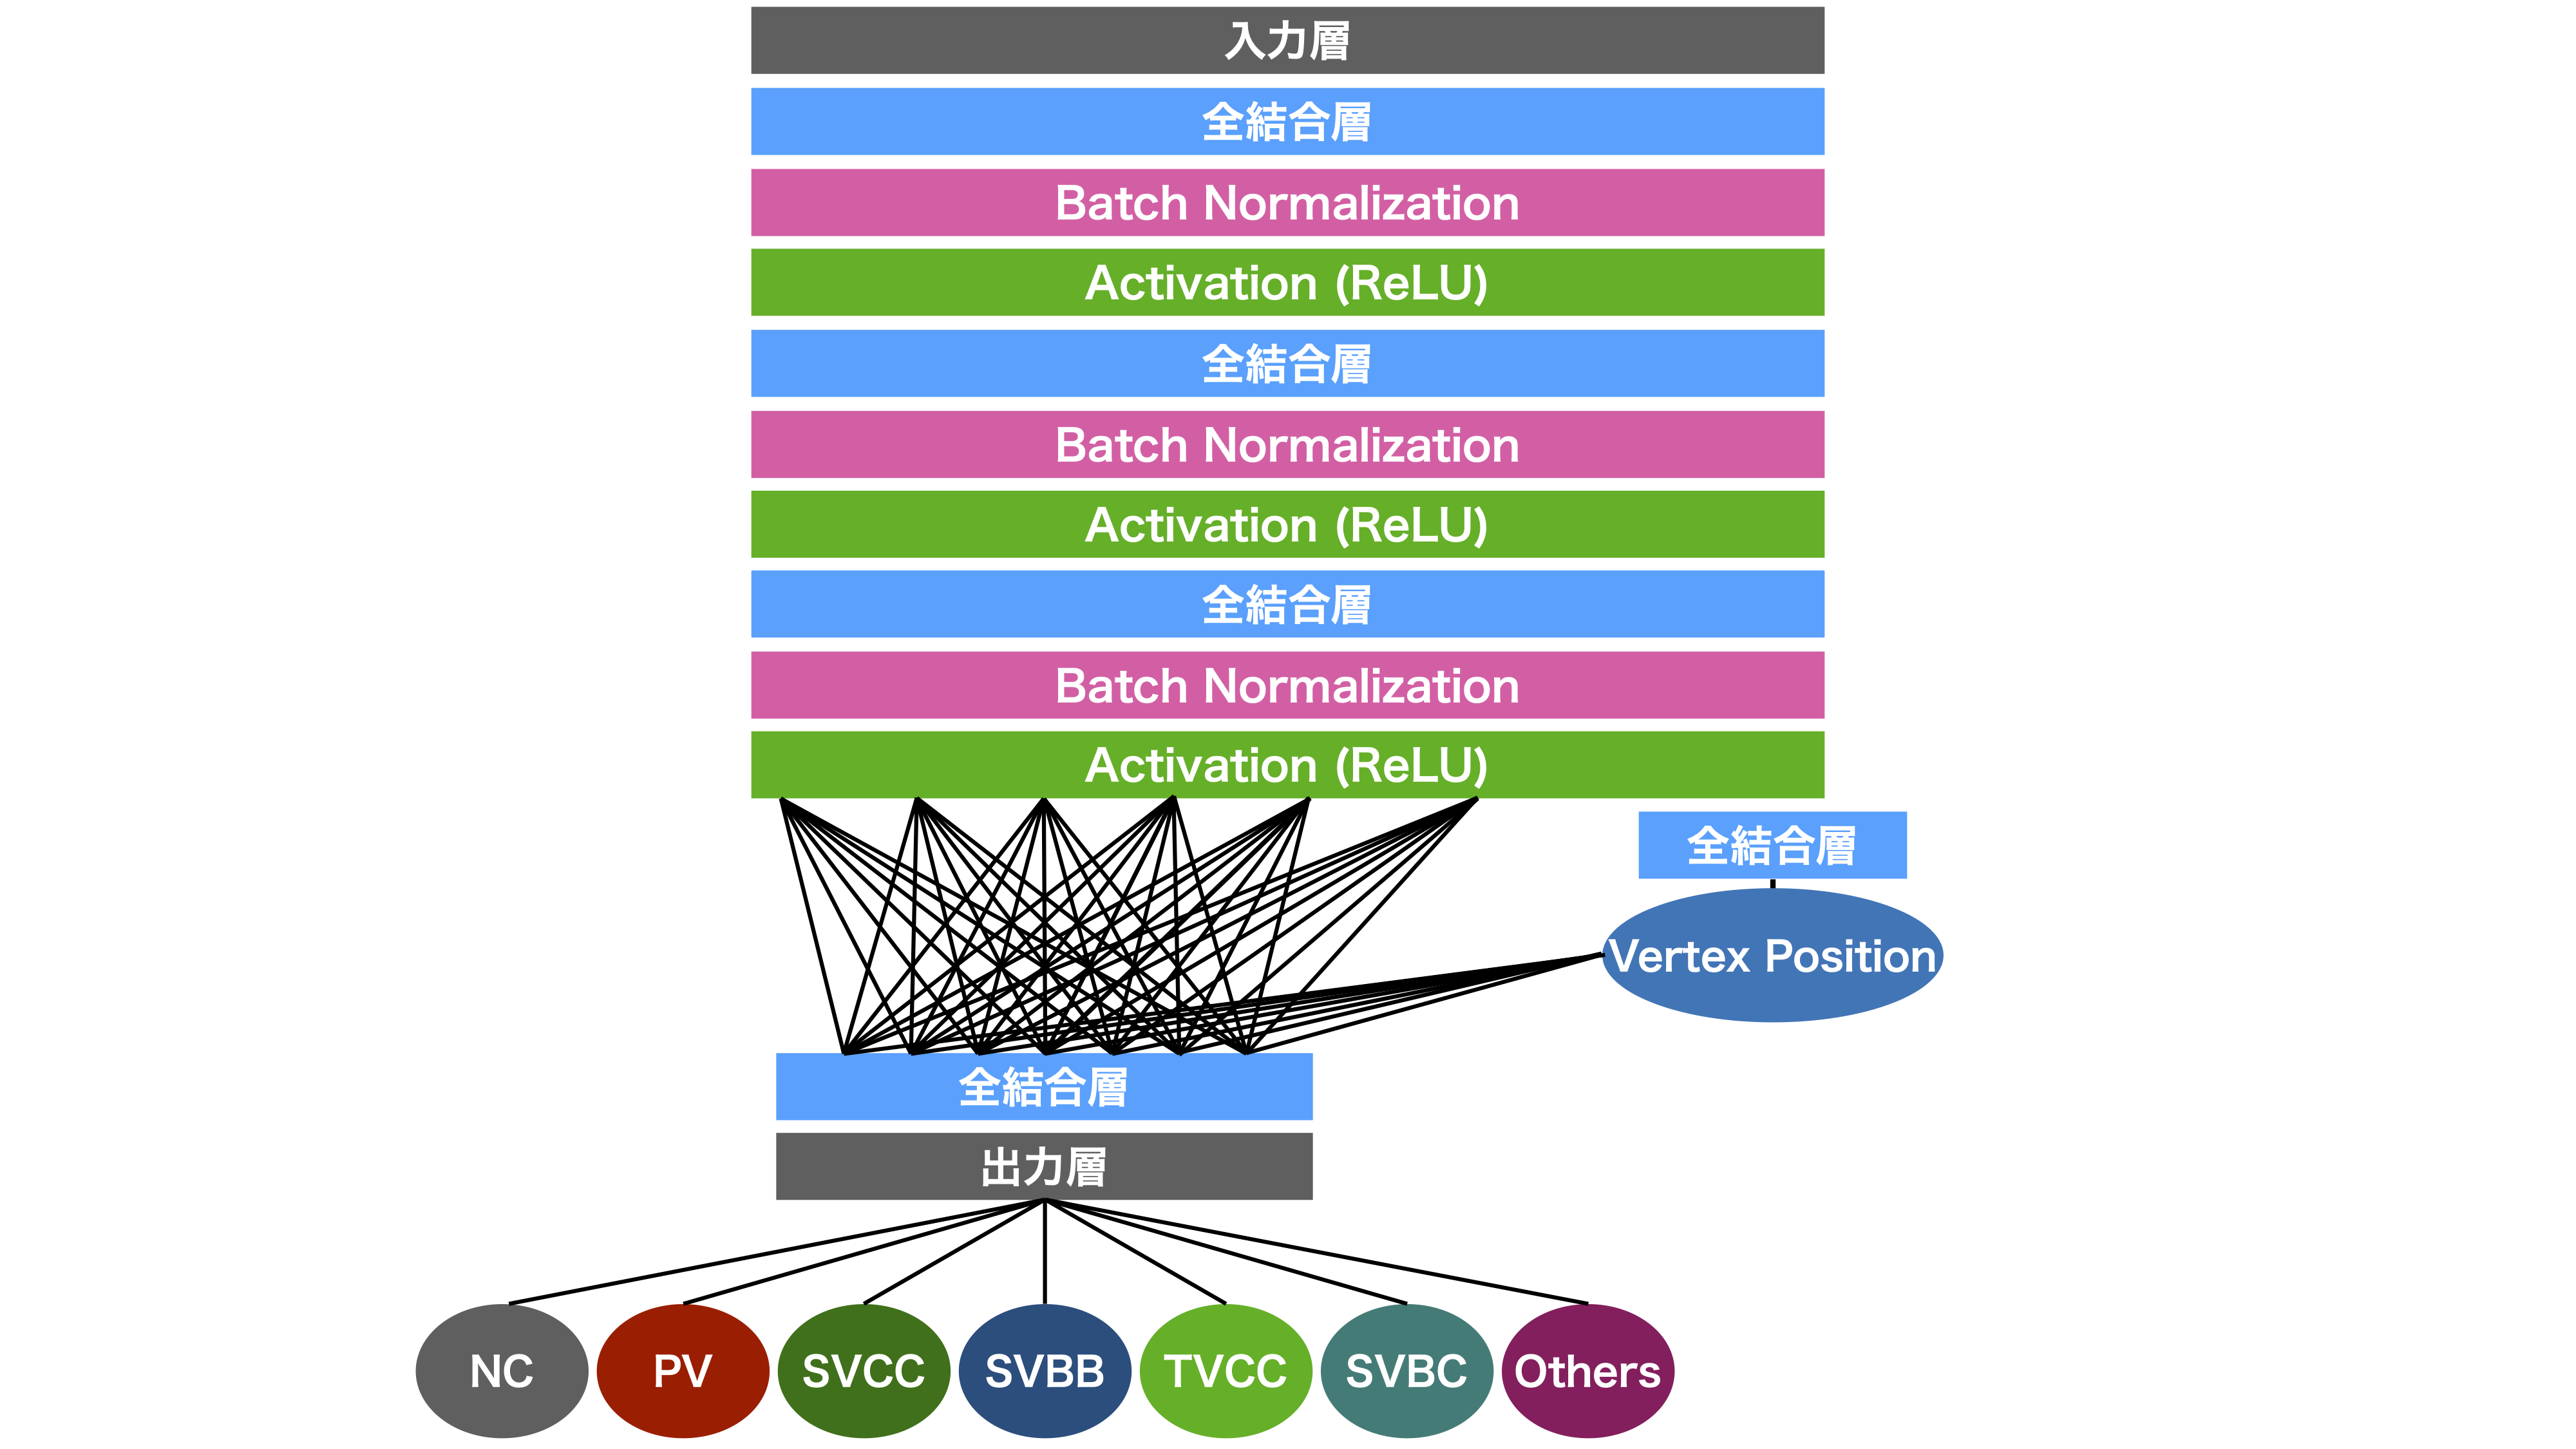
\includegraphics[trim = 200 0 200 0, width=1.0\textwidth, clip]{Figure/3Networks/3-3-3-1PairNetworkB.png}
    \subcaption{ネットワーク3}
    \label{3-3-3-1PairNetworkB}
   \end{minipage}
  \end{minipage}  
  \caption{評価のための飛跡対についてのネットワーク}
  \label{3-3-3-1PairNetworks}
 %\end{tabular}
\end{figure}

\begin{table}[htb]
 \centering
 \small
  \begin{tabular*}{1.0\textwidth}{@{\extracolsep{\fill}}c c c}\hline
    モデル & 入力変数 & ネットワーク\\\hline\hline
    モデルA & トラック・パラメータ, 共分散行列, 電荷, エネルギー & ネットワーク1\\
    モデルB & トラック・パラメータ, 電荷, エネルギー & ネットワーク1\\
    モデルC & トラック・パラメータ, 共分散行列, 電荷, エネルギー, 崩壊点の位置 & ネットワーク2\\
    モデルD & トラック・パラメータ, 共分散行列, 電荷, エネルギー & ネットワーク3\\\hline
  \end{tabular*}
  \caption{評価のための飛跡対についてのモデル}
  \label{EvalationModels}
\end{table}

比較は各クラス分類についての「ネットワークのスコアとその効率の変化」と「混合行列」の二つの指標を用いて行う。
また, 本ネットワークは7クラス分類を行っているため, ある特定のクラスについてのスコアに閾値を設け, 評価することは数学的に厳密に正しくない。
しかし, ここでは直感的な理解を優先し評価手法の一つとして採用している。

まず, ネットワークのスコアとクラス分類の効率の関係を図\ref{3-3-3-2Efficiency_Curve}に示す。
図の横軸はネットワークによって得られる各クラスのスコアに設けた閾値である。
また, 縦軸は効率を示しており, 実線で信号効率を, 破線でバックグラウンド効率を表している。
ここでは, 信号はそれぞれの特定のクラスとし, バックグラウンドはその特定のクラス以外の全てのクラスと定義している。
スコアに対して高い閾値を設けると信号・バックグラウンド共に効率は悪化し, 逆に低い閾値であれば, 全ての要素を信号であると判断してしまうため, 両者の効率は最大となっている。
したがって, 高い信号効率と低いバックグラウンド効率を実現できていれば, 良い分類器であると判断できる。
図\ref{3-3-3-2Efficiency_Curve}ではNC・PV・Othersについては良く分類できているが, 各SVについては殆ど見分けられていないことが分かる。

\begin{figure}[htbp]
 \centering
  %\begin{tabular}{cccc}
   \begin{minipage}{1.0\textwidth}
    \centering
    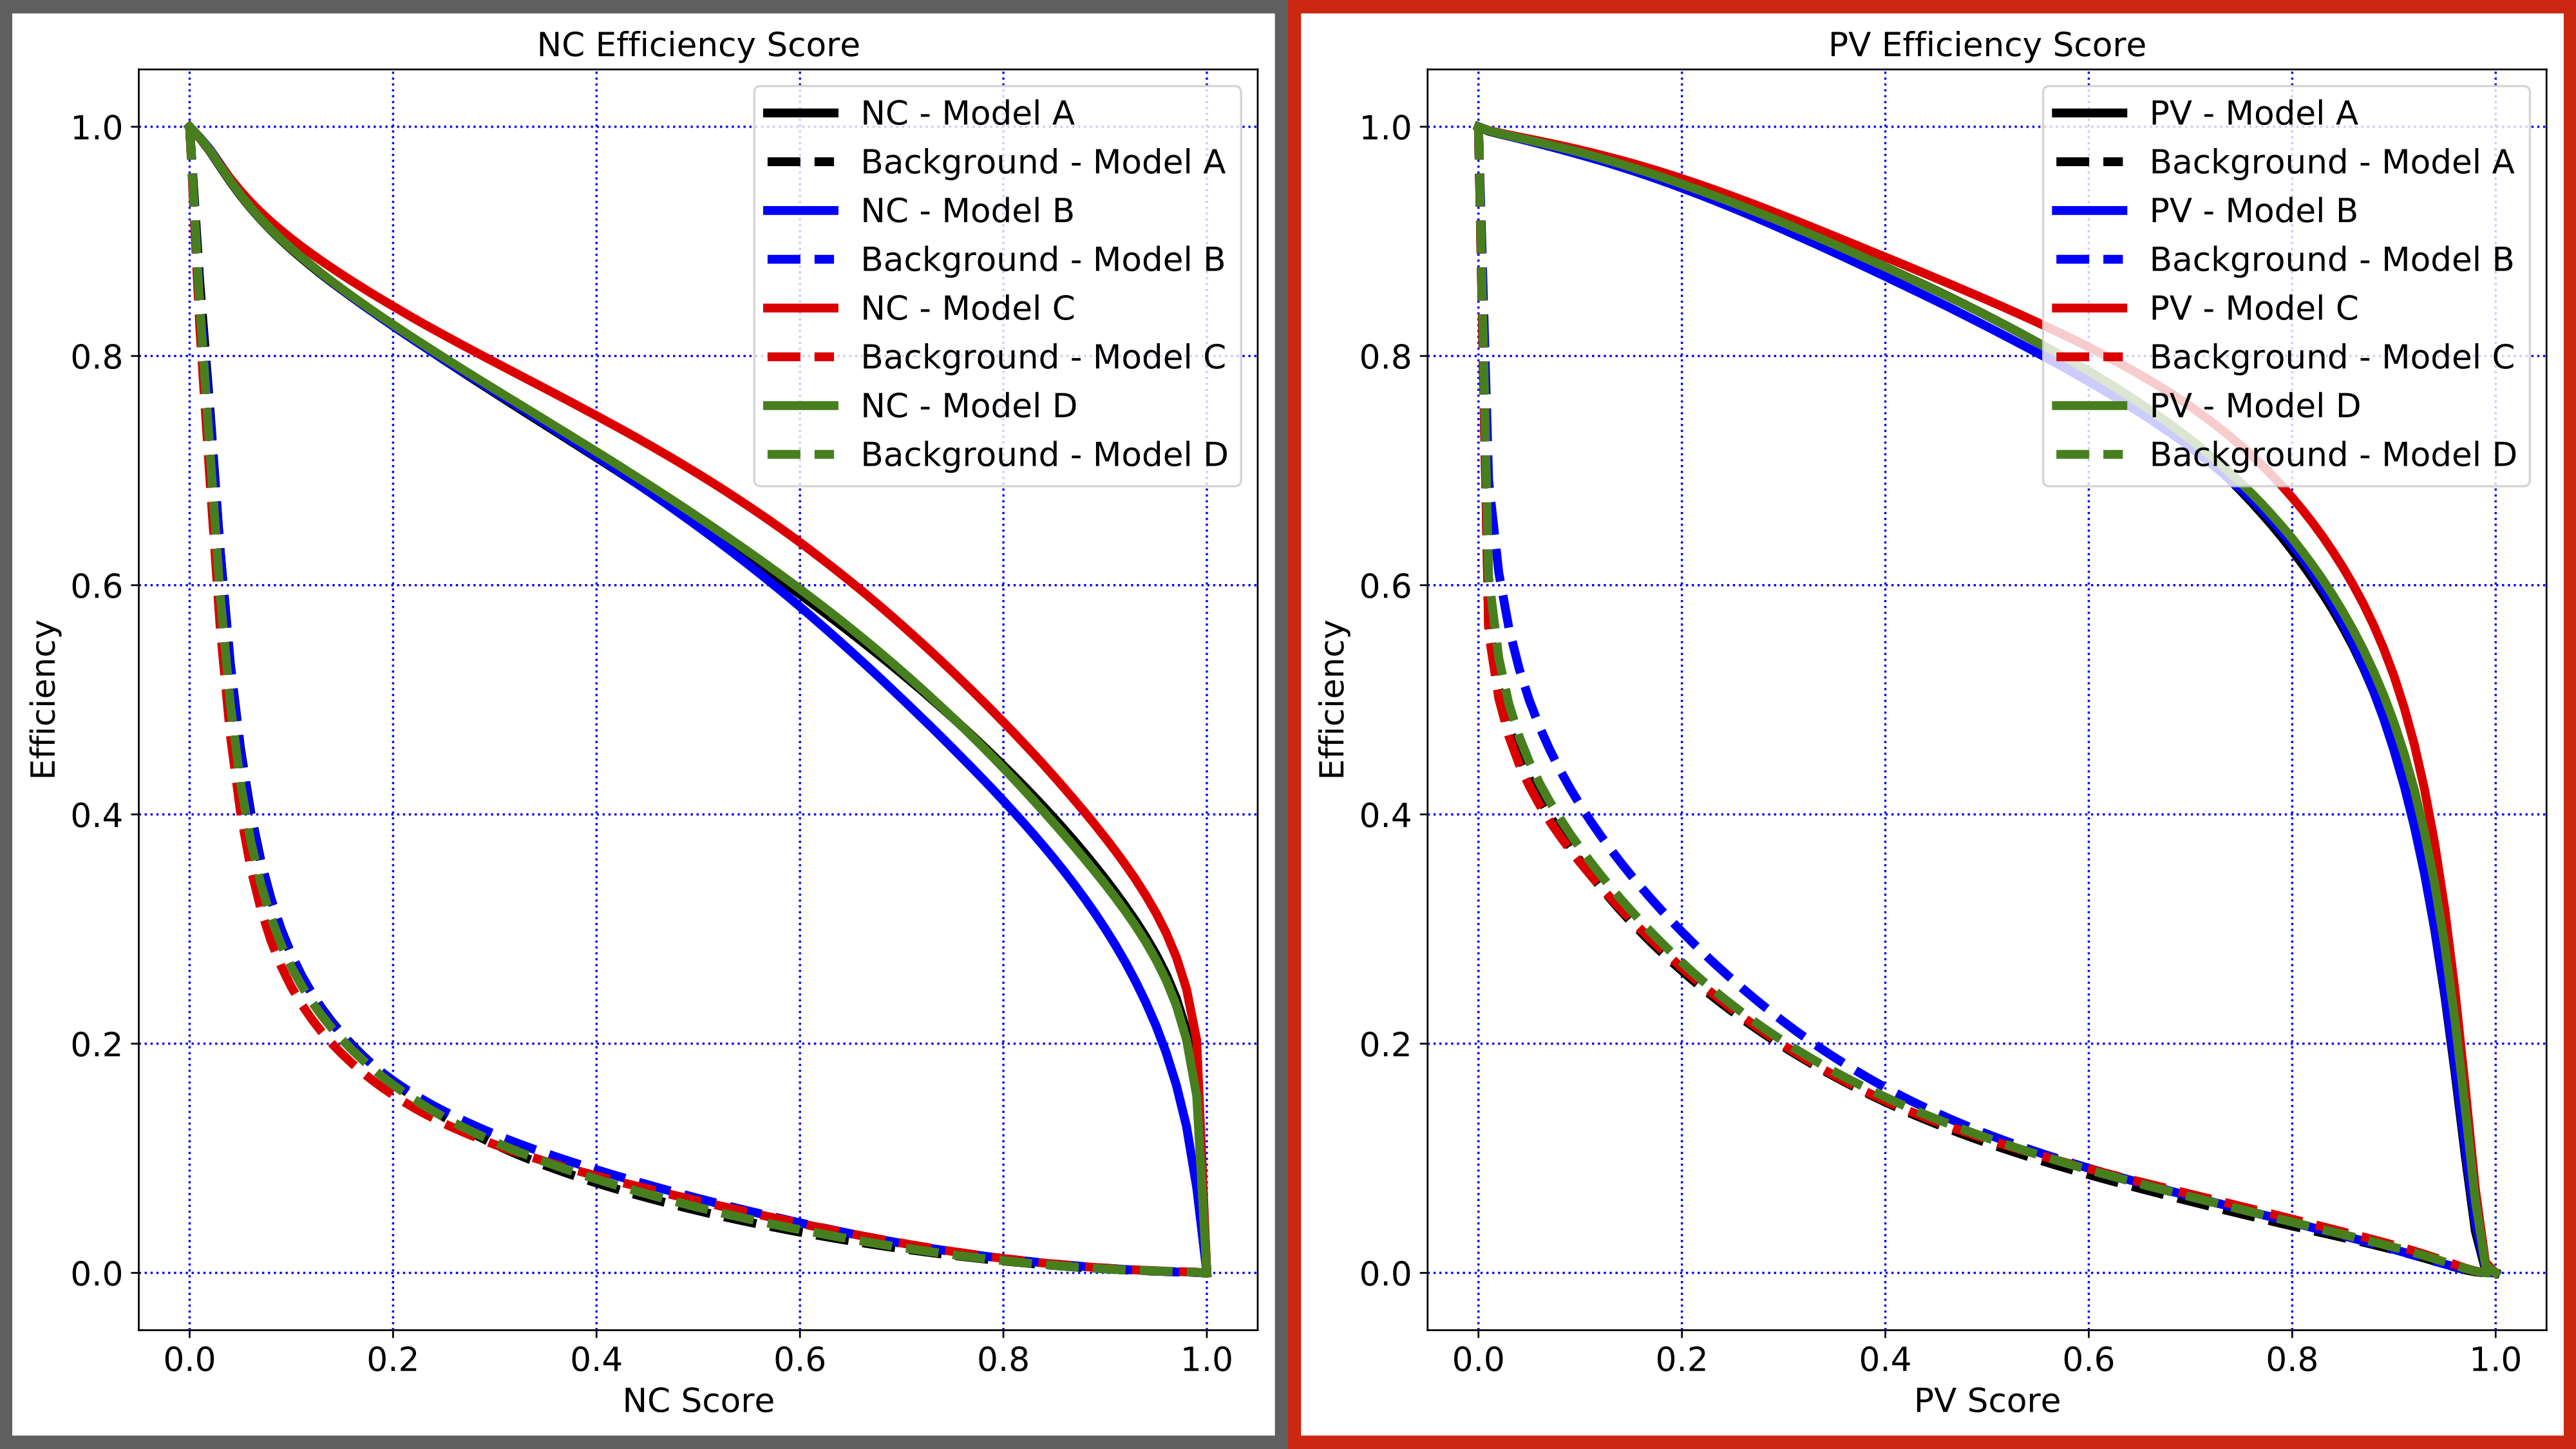
\includegraphics[width=1.0\textwidth, clip]{Figure/3Networks/3-3-3-2Efficiency_Curve_1.png}
   \end{minipage}

   \begin{minipage}{1.0\textwidth}
   \centering
    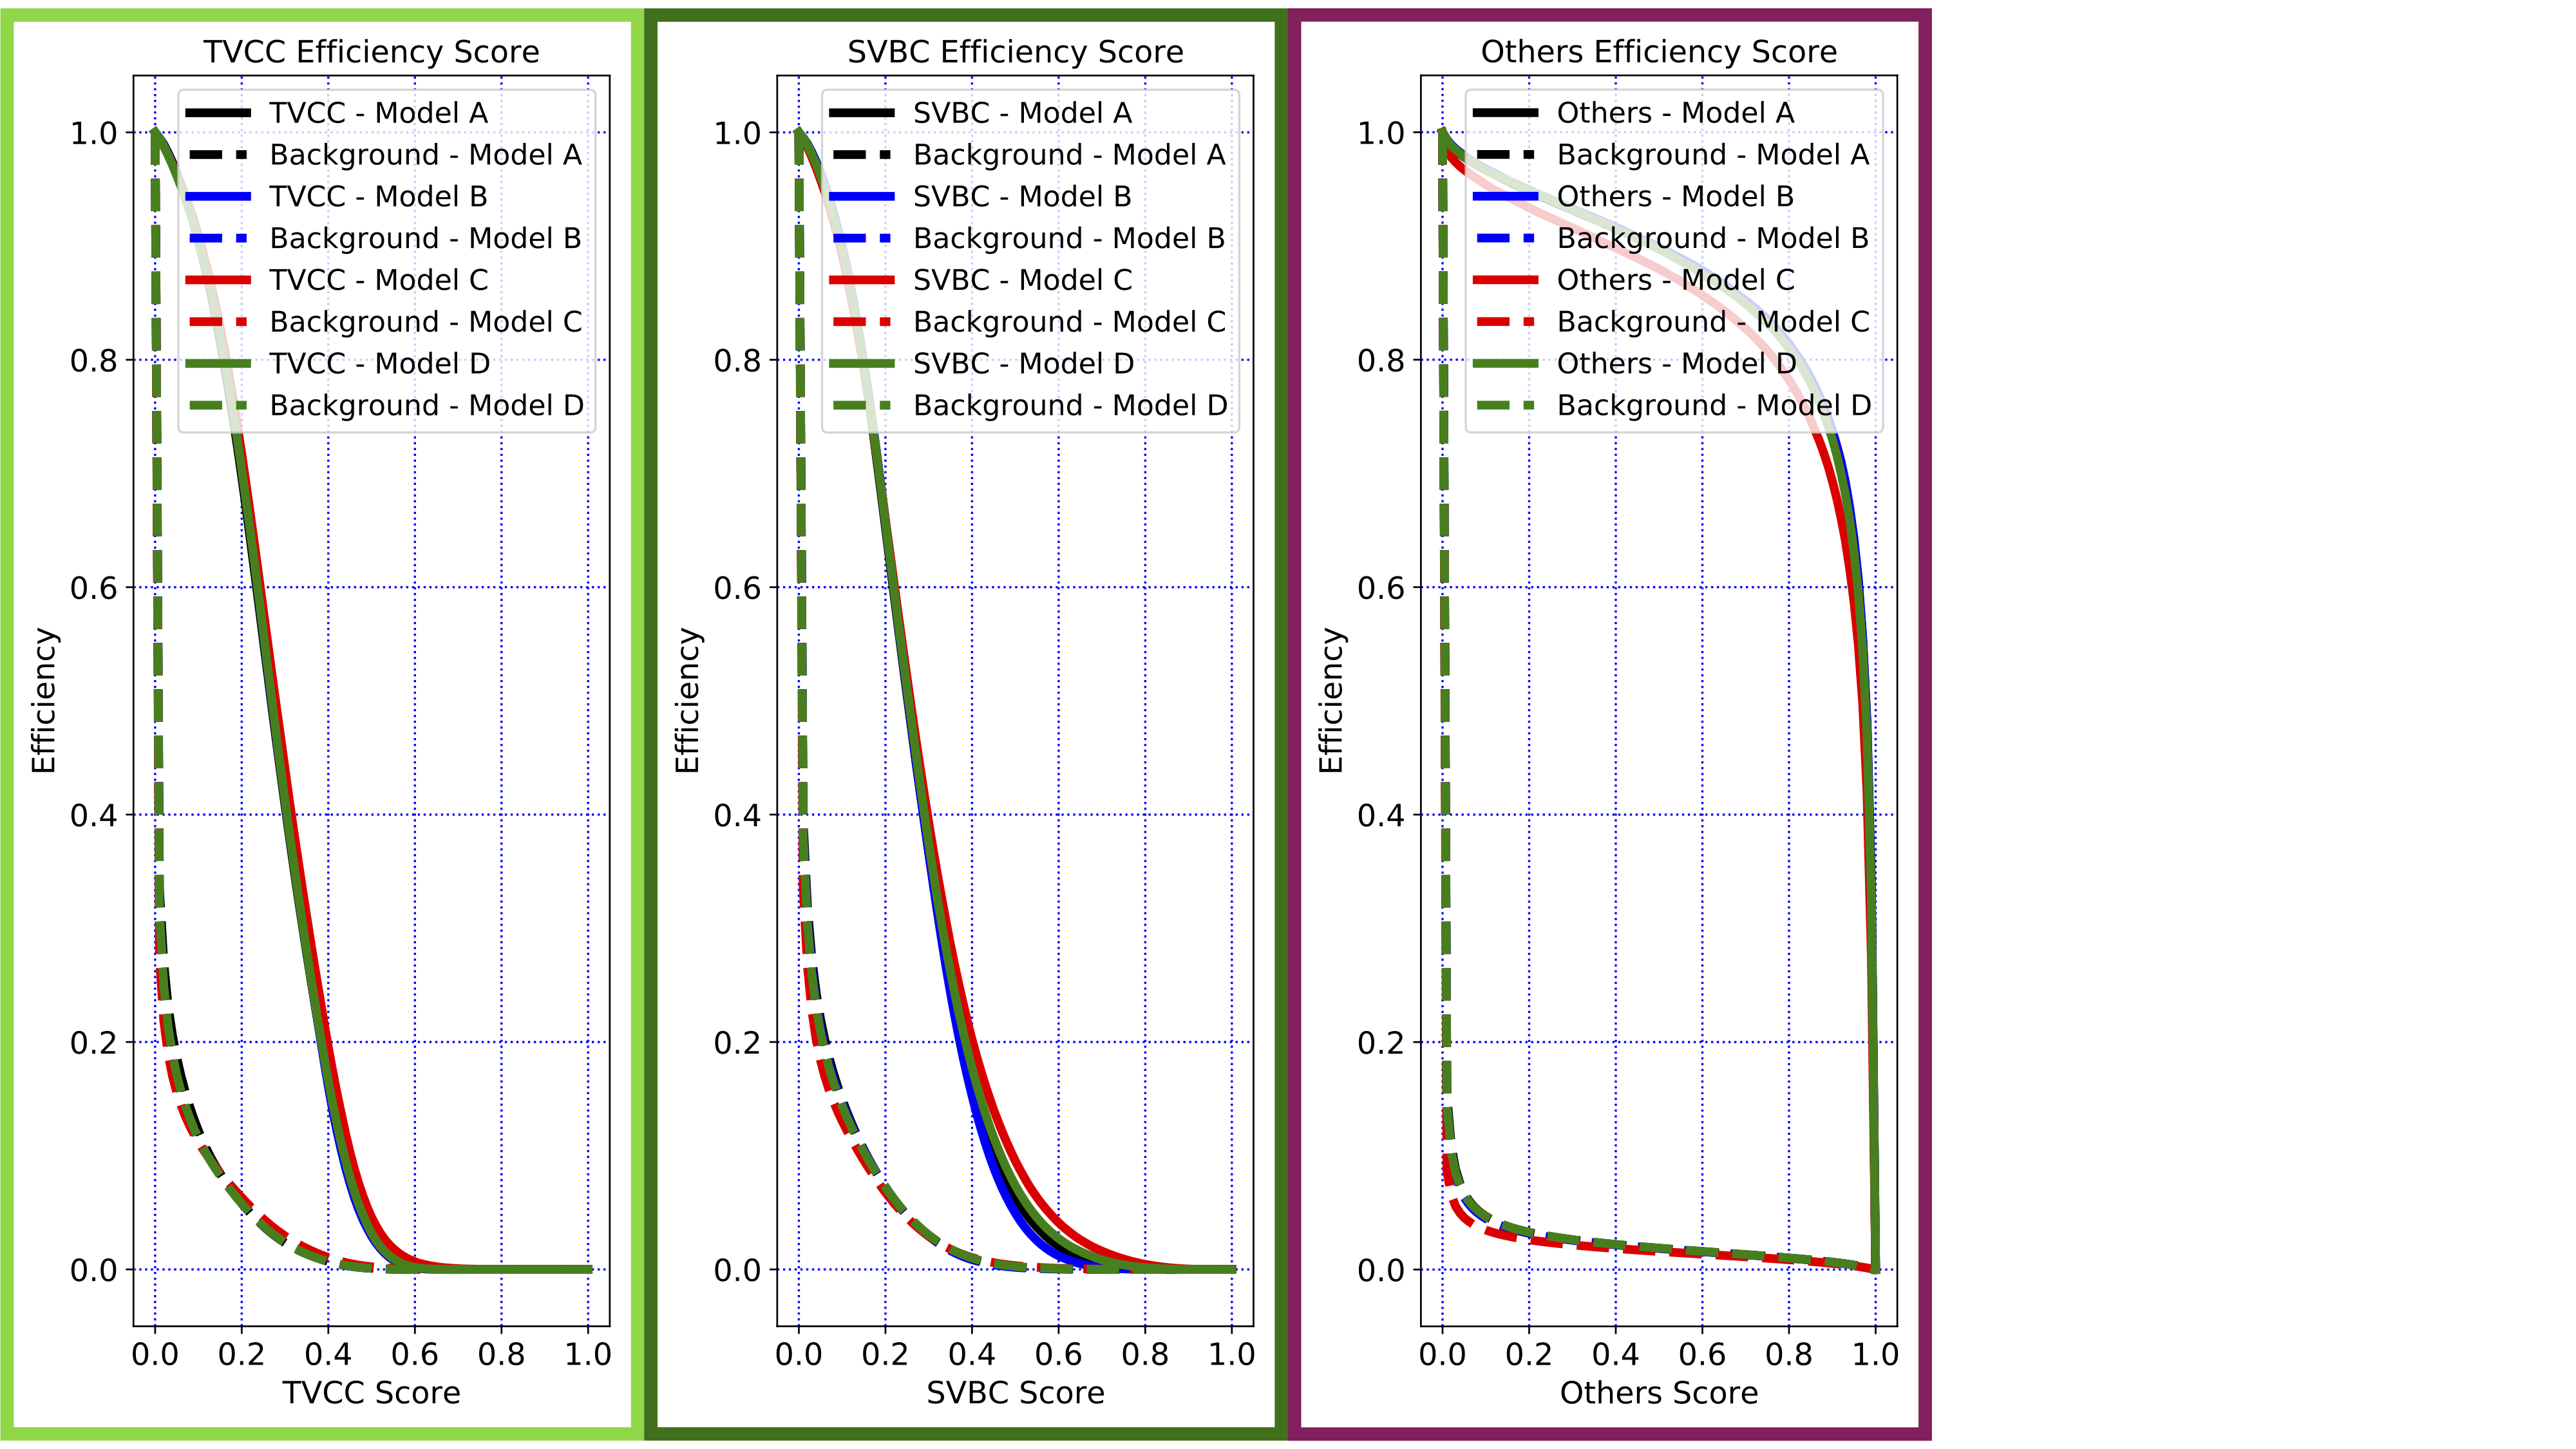
\includegraphics[width=1.0\textwidth, clip]{Figure/3Networks/3-3-3-2Efficiency_Curve_2.png}
   \end{minipage}
  \caption[ネットワークのスコアとクラス分類の効率の関係]{ネットワークのスコアとクラス分類の効率の関係。縦軸は効率, 横軸はネットワークのスコアについての閾値である。実線は信号効率, 破線はバックグラウンド効率である。黒線はモデルA, 青線はモデルB, 赤線はモデルC, 緑線はモデルDをそれぞれ表している。}
  \label{3-3-3-2Efficiency_Curve}
 %\end{tabular}
\end{figure}

これら信号効率を縦軸にバックグラウンド効率を横軸に描画したものが図\ref{3-3-3-2ROC_Curve}である。
このような図を受信者操作特性(Receiver Operating Characteristic, ROC)曲線といい, ROC曲線はその曲線で囲んだ面積が大きければ性能が良いと判断できる。
したがって, より左側に張り出している分類器が最も良い性能となる。
ここでは, 横軸を対数で表現しており, よりバックグラウンド効率の低い領域において, それぞれのモデルの比較を行っている。
図\ref{3-3-3-2ROC_Curve}ではどのクラスについてのモデル間の大きさ差異は見られない。
ただし, NCについてのみModel Bの性能が悪いという結果を得られた。

\begin{figure}[htbp]
 \centering
  %\begin{tabular}{cccc}
  \begin{minipage}{1.0\textwidth}
   \centering
    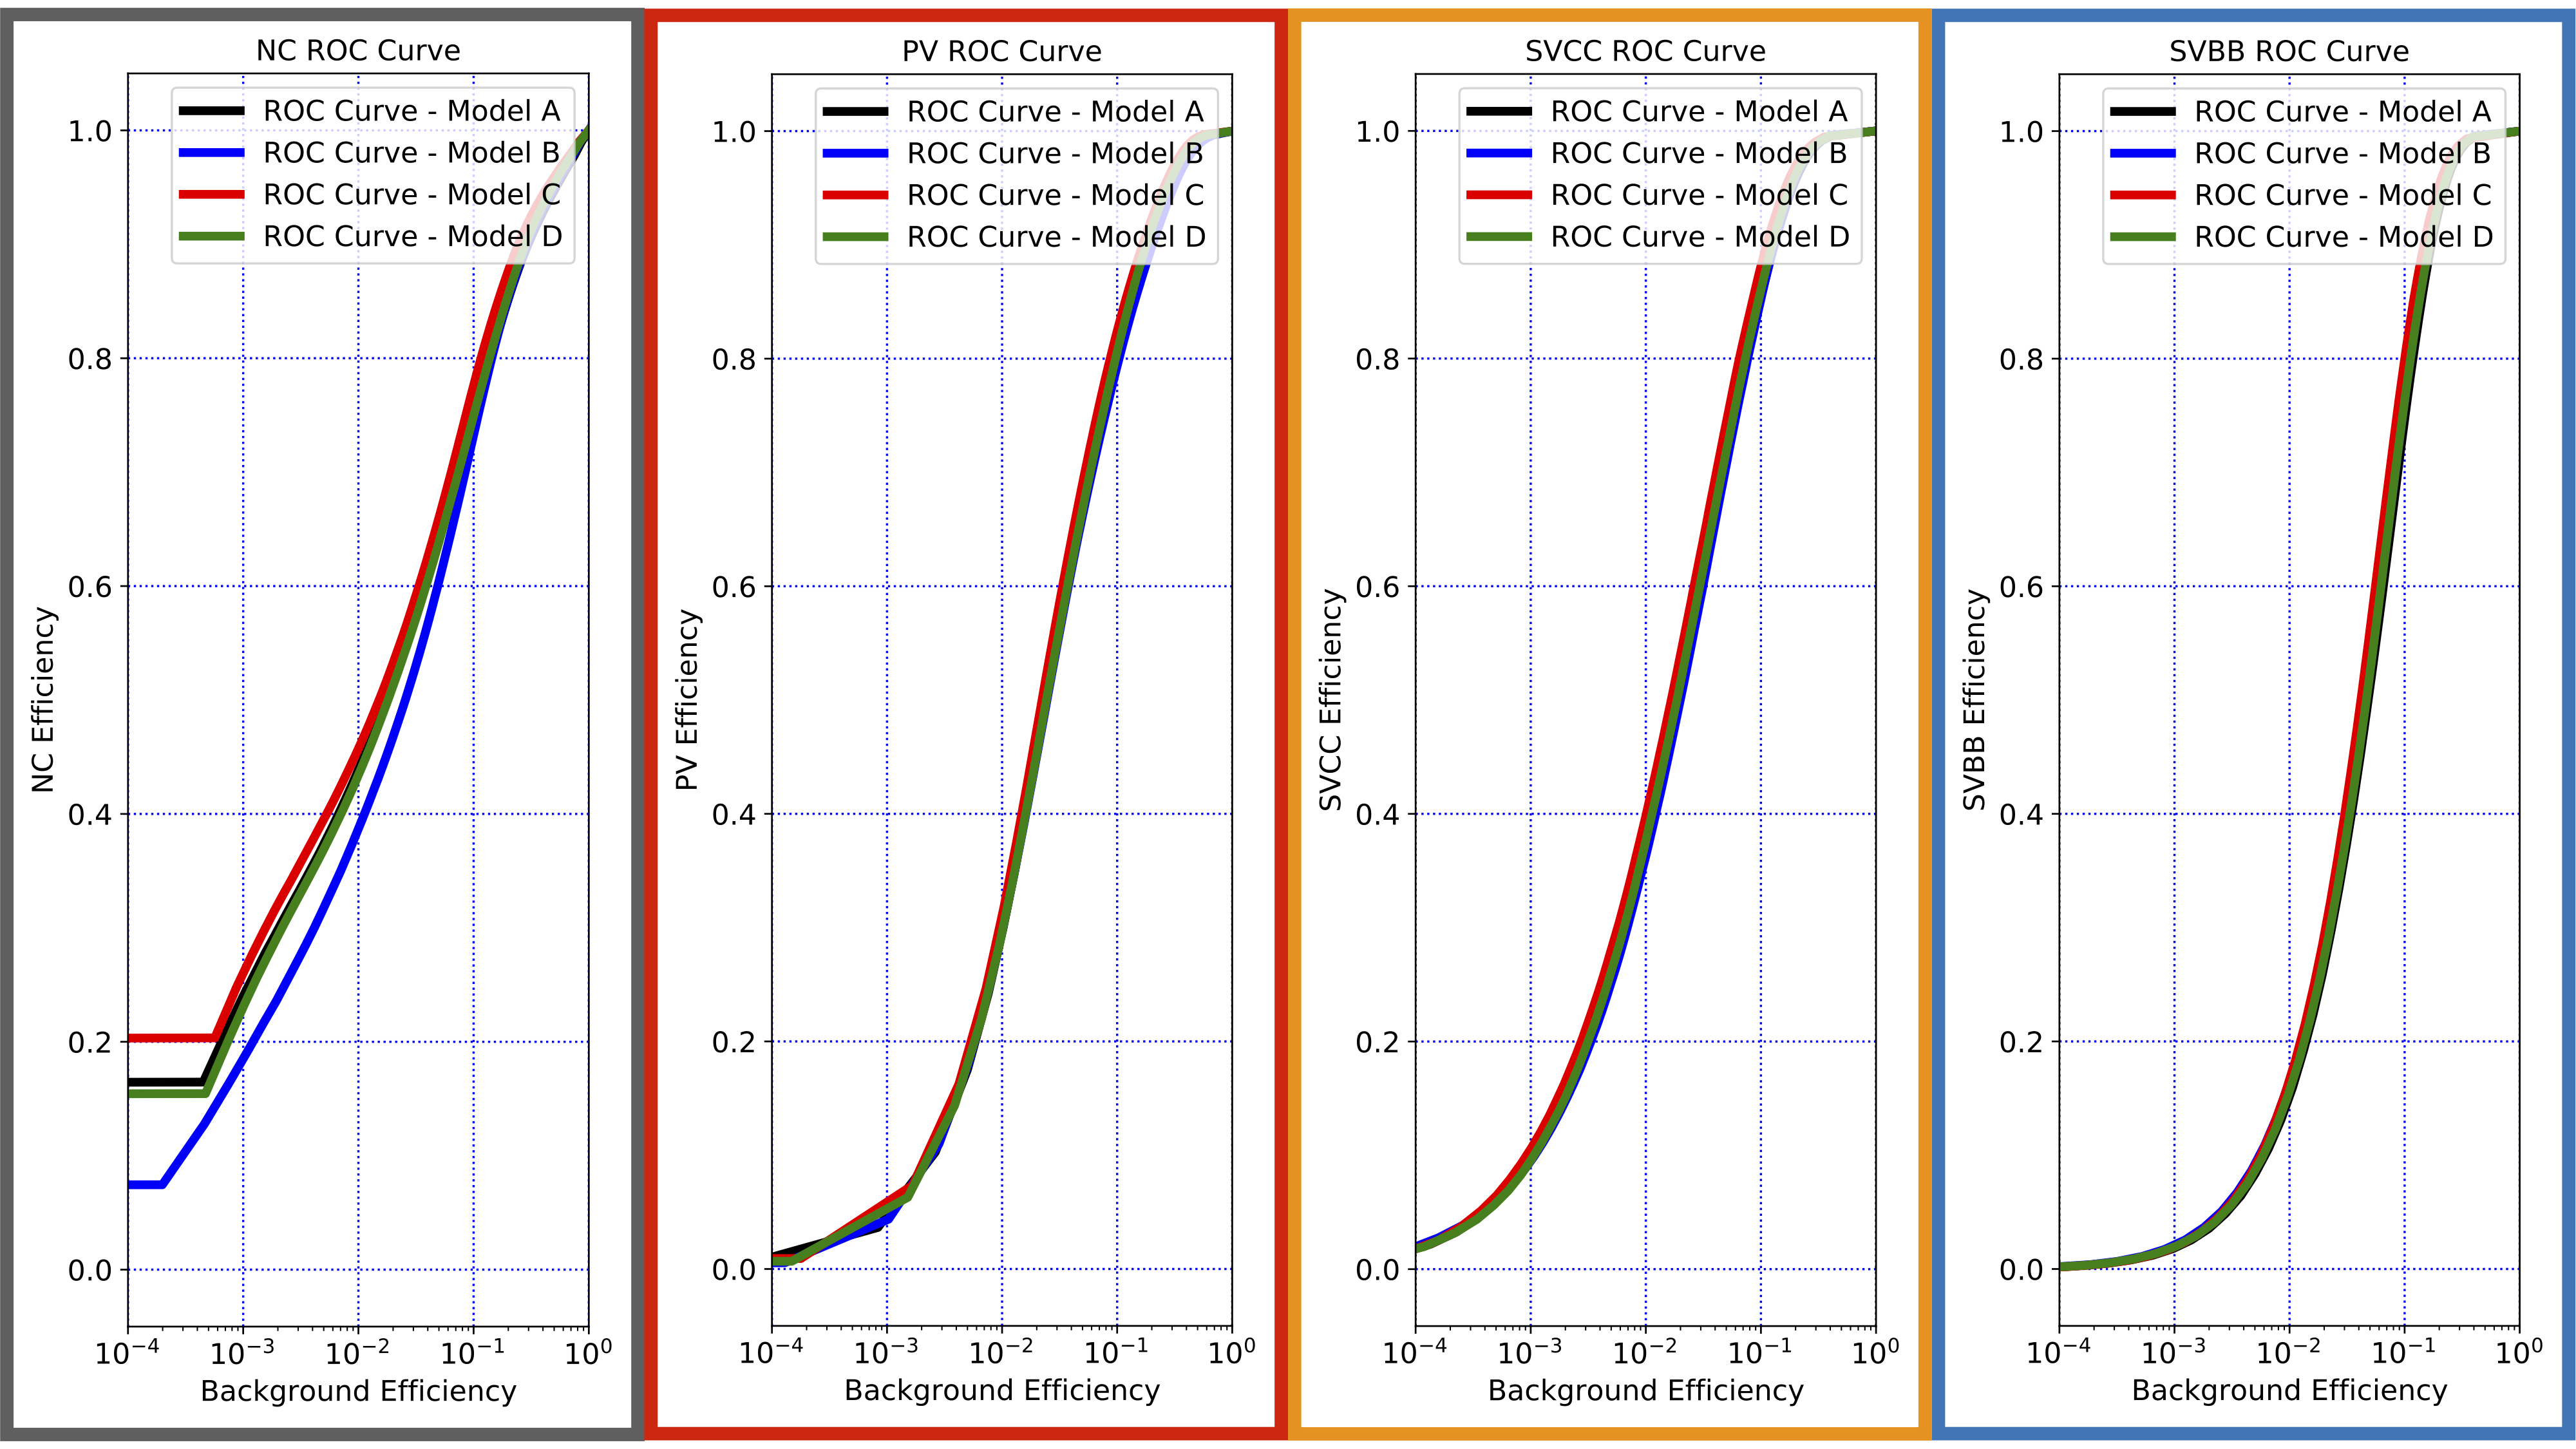
\includegraphics[width=1.0\textwidth, clip]{Figure/3Networks/3-3-3-2ROC_Curve_1.png}
   \end{minipage}
   
   \begin{minipage}{1.0\textwidth}
   \centering
    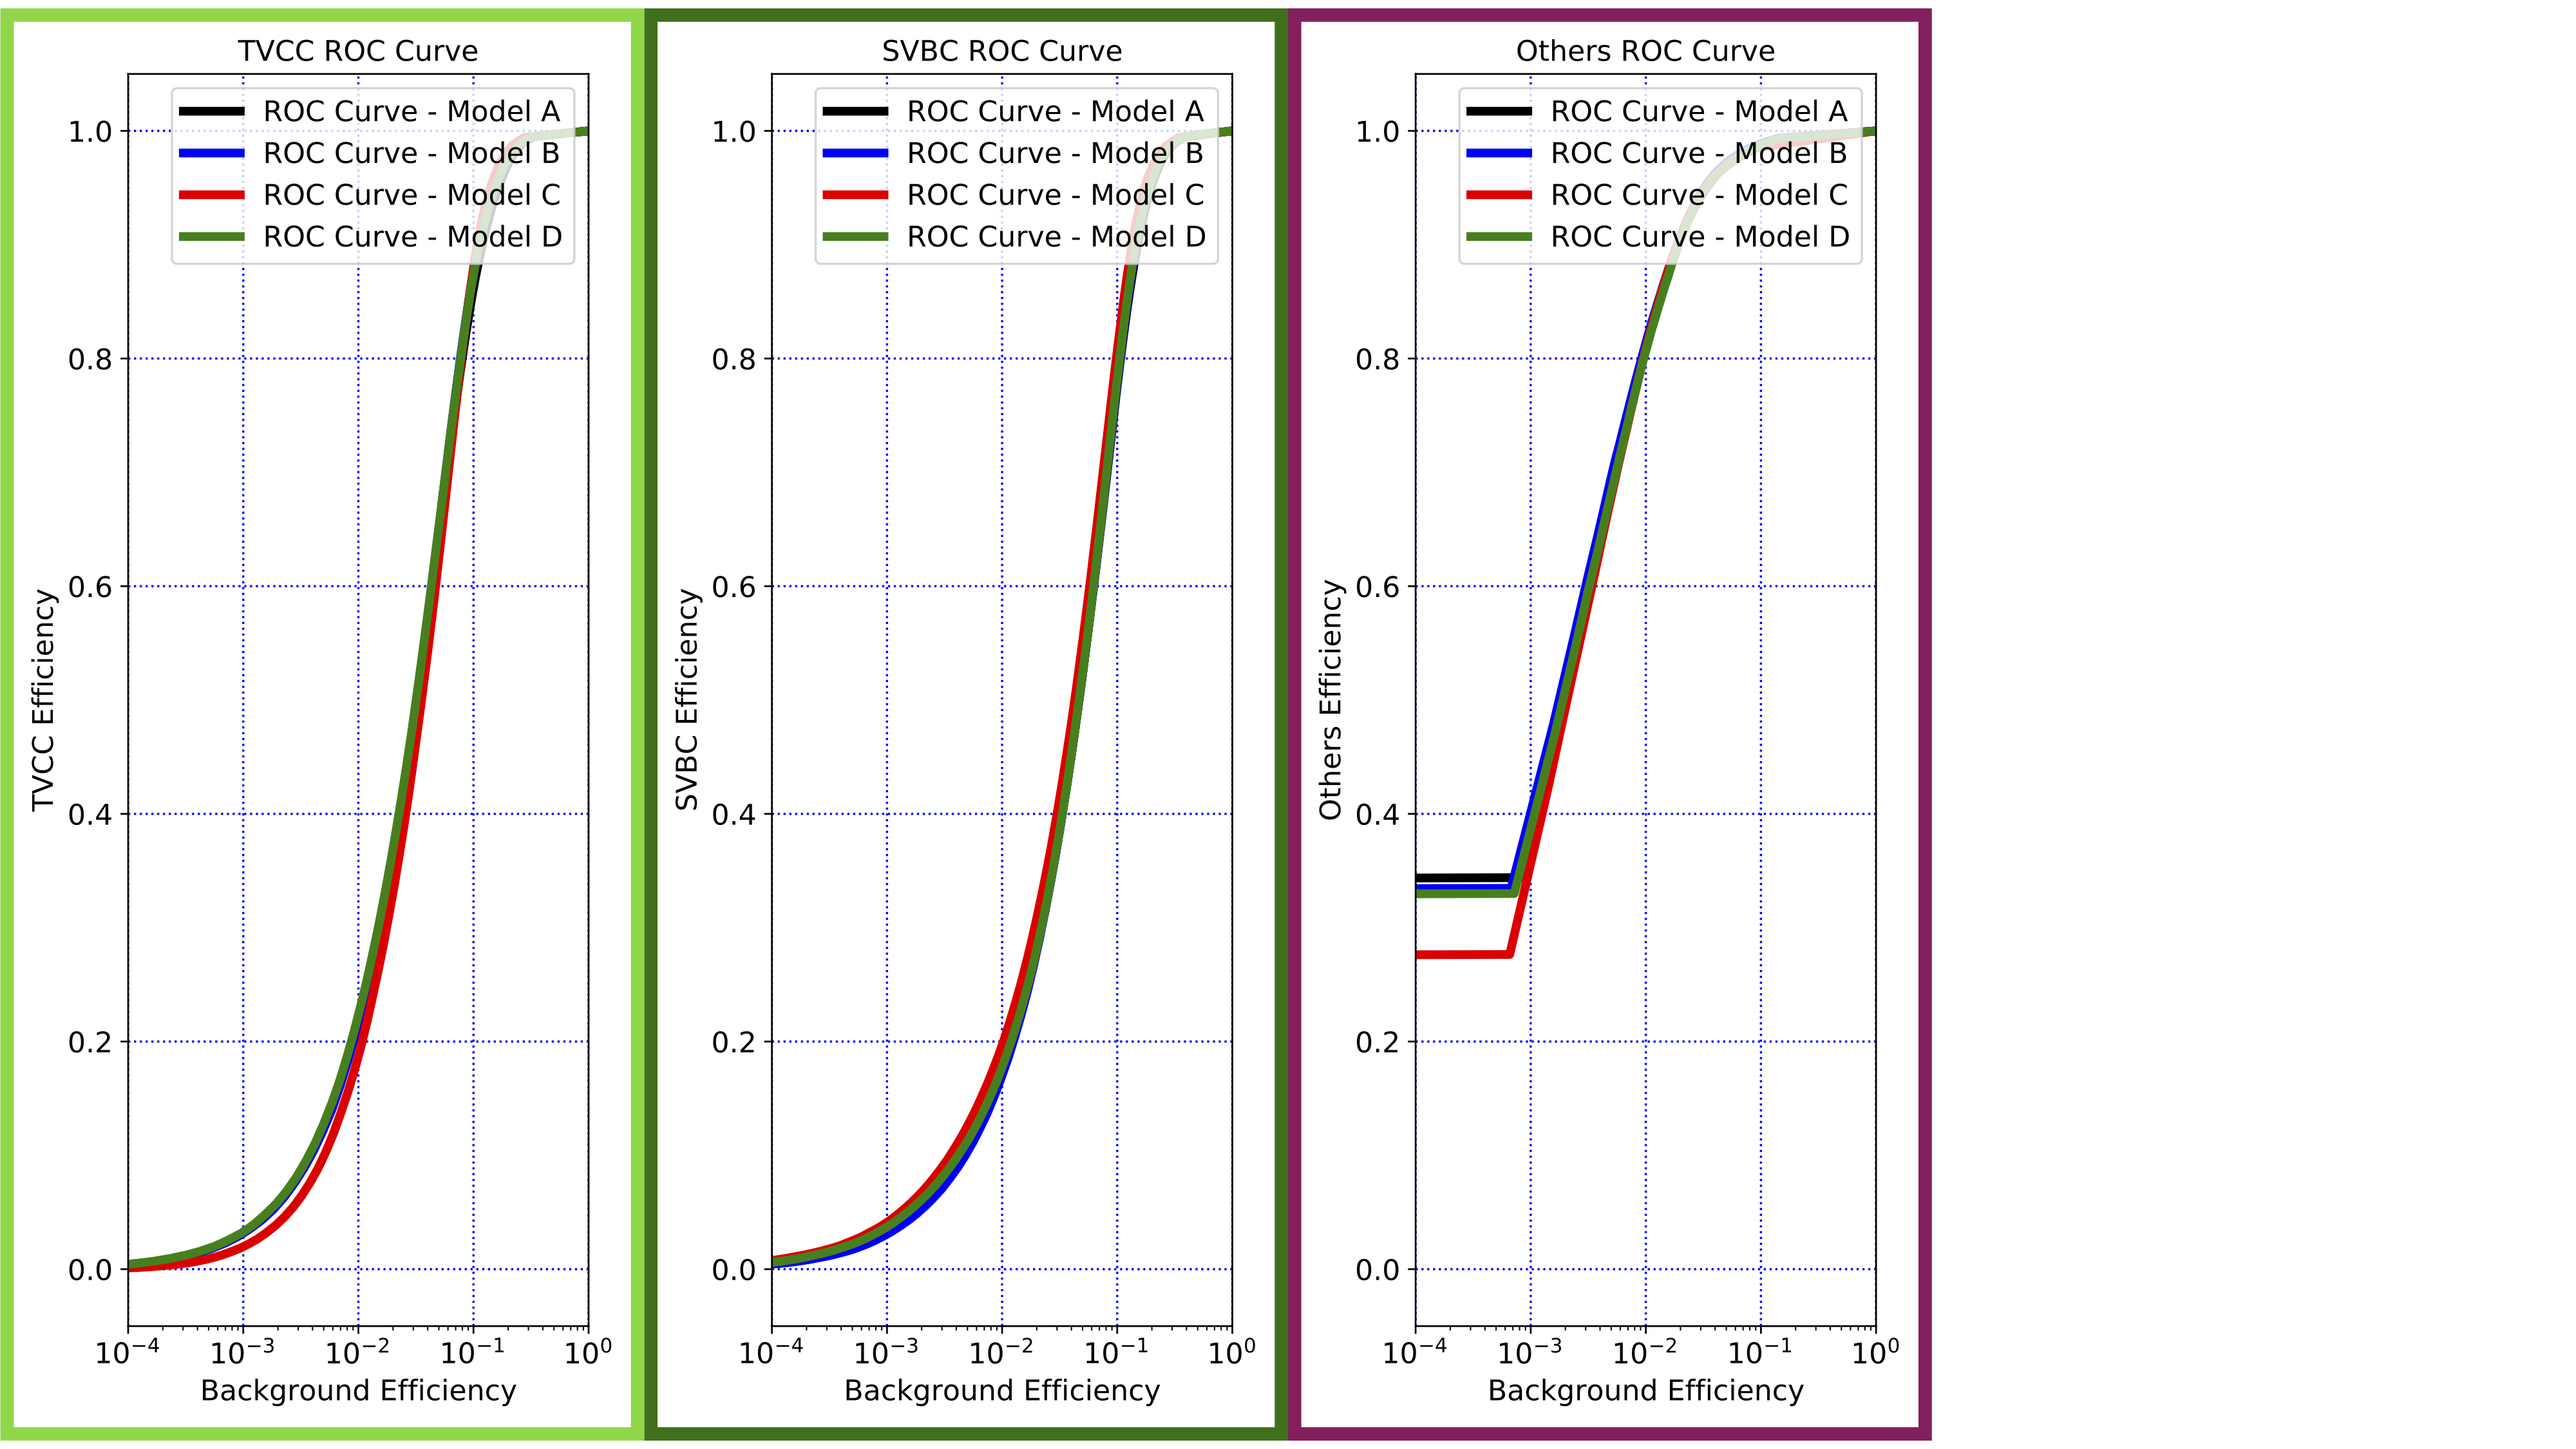
\includegraphics[width=1.0\textwidth, clip]{Figure/3Networks/3-3-3-2ROC_Curve_2.png}
   \end{minipage}
  \caption[各モデルのROC曲線]{各モデルのROC曲線。縦軸は信号効率, 横軸はバックグラウンド効率である。黒線はモデルA, 青線はモデルB, 赤線はモデルC, 緑線はモデルDをそれぞれ表している。}
  \label{3-3-3-2ROC_Curve}
 %\end{tabular}
\end{figure}

ネットワークがどの程度の効率や純度でクラスを分類出来ているかを更に把握するため混合行列を用いる(図\ref{3-3-3-2ConfusionMatrix})。
混合行列は横軸をネットワークによって予想されたクラス, 縦軸を正解ラベルでのクラスとしてデータを行列化したものである。
したがって, 対角成分が正答, それ以外は誤答である。
ここでは, 効率について規格化したものと純度について規格化したものの二つで評価を行う。
また, 比較のためモデルB,C,Dの結果についてはモデルAとの相対値で表している。

\begin{figure}[htbp]
 \centering
  %\begin{tabular}{cccc}
  \begin{minipage}{1.0\textwidth}
   \centering
    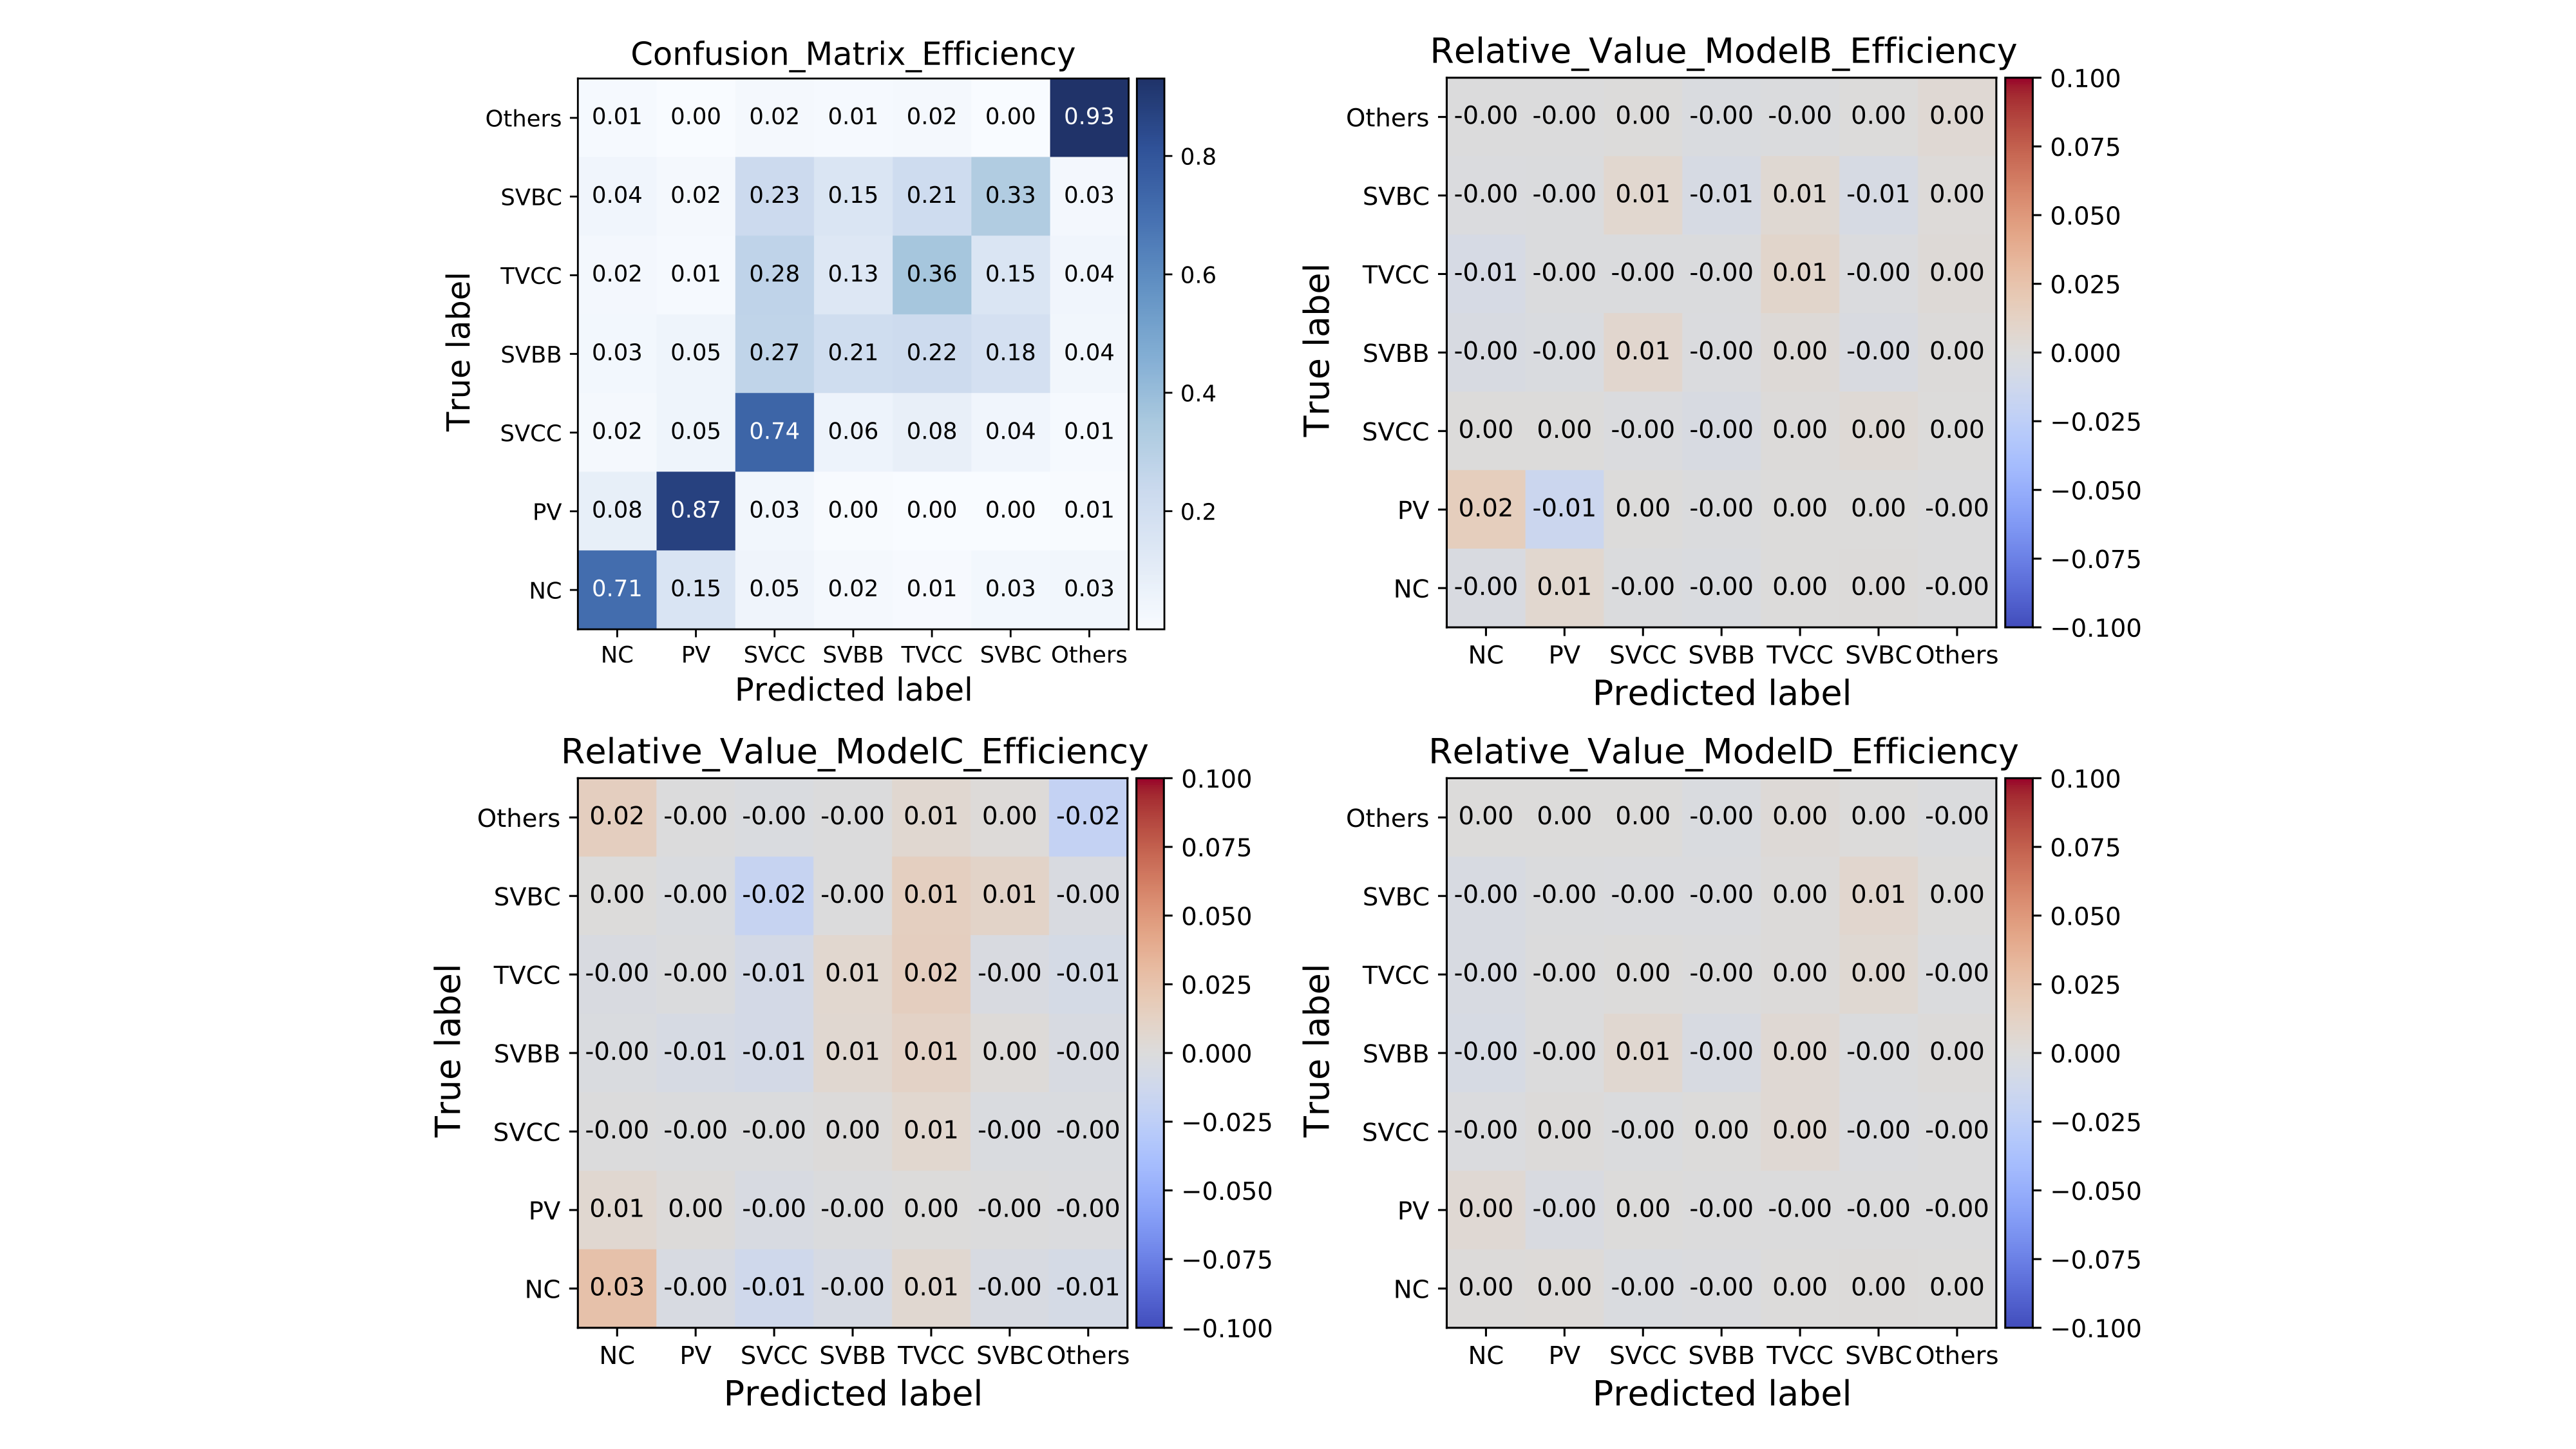
\includegraphics[trim = 300 0 300 0, width=0.9\textwidth, clip]{Figure/3Networks/3-3-3-2ConfusionMatrix_1.png}
   \end{minipage}
   
   \begin{minipage}{1.0\textwidth}
   \centering
    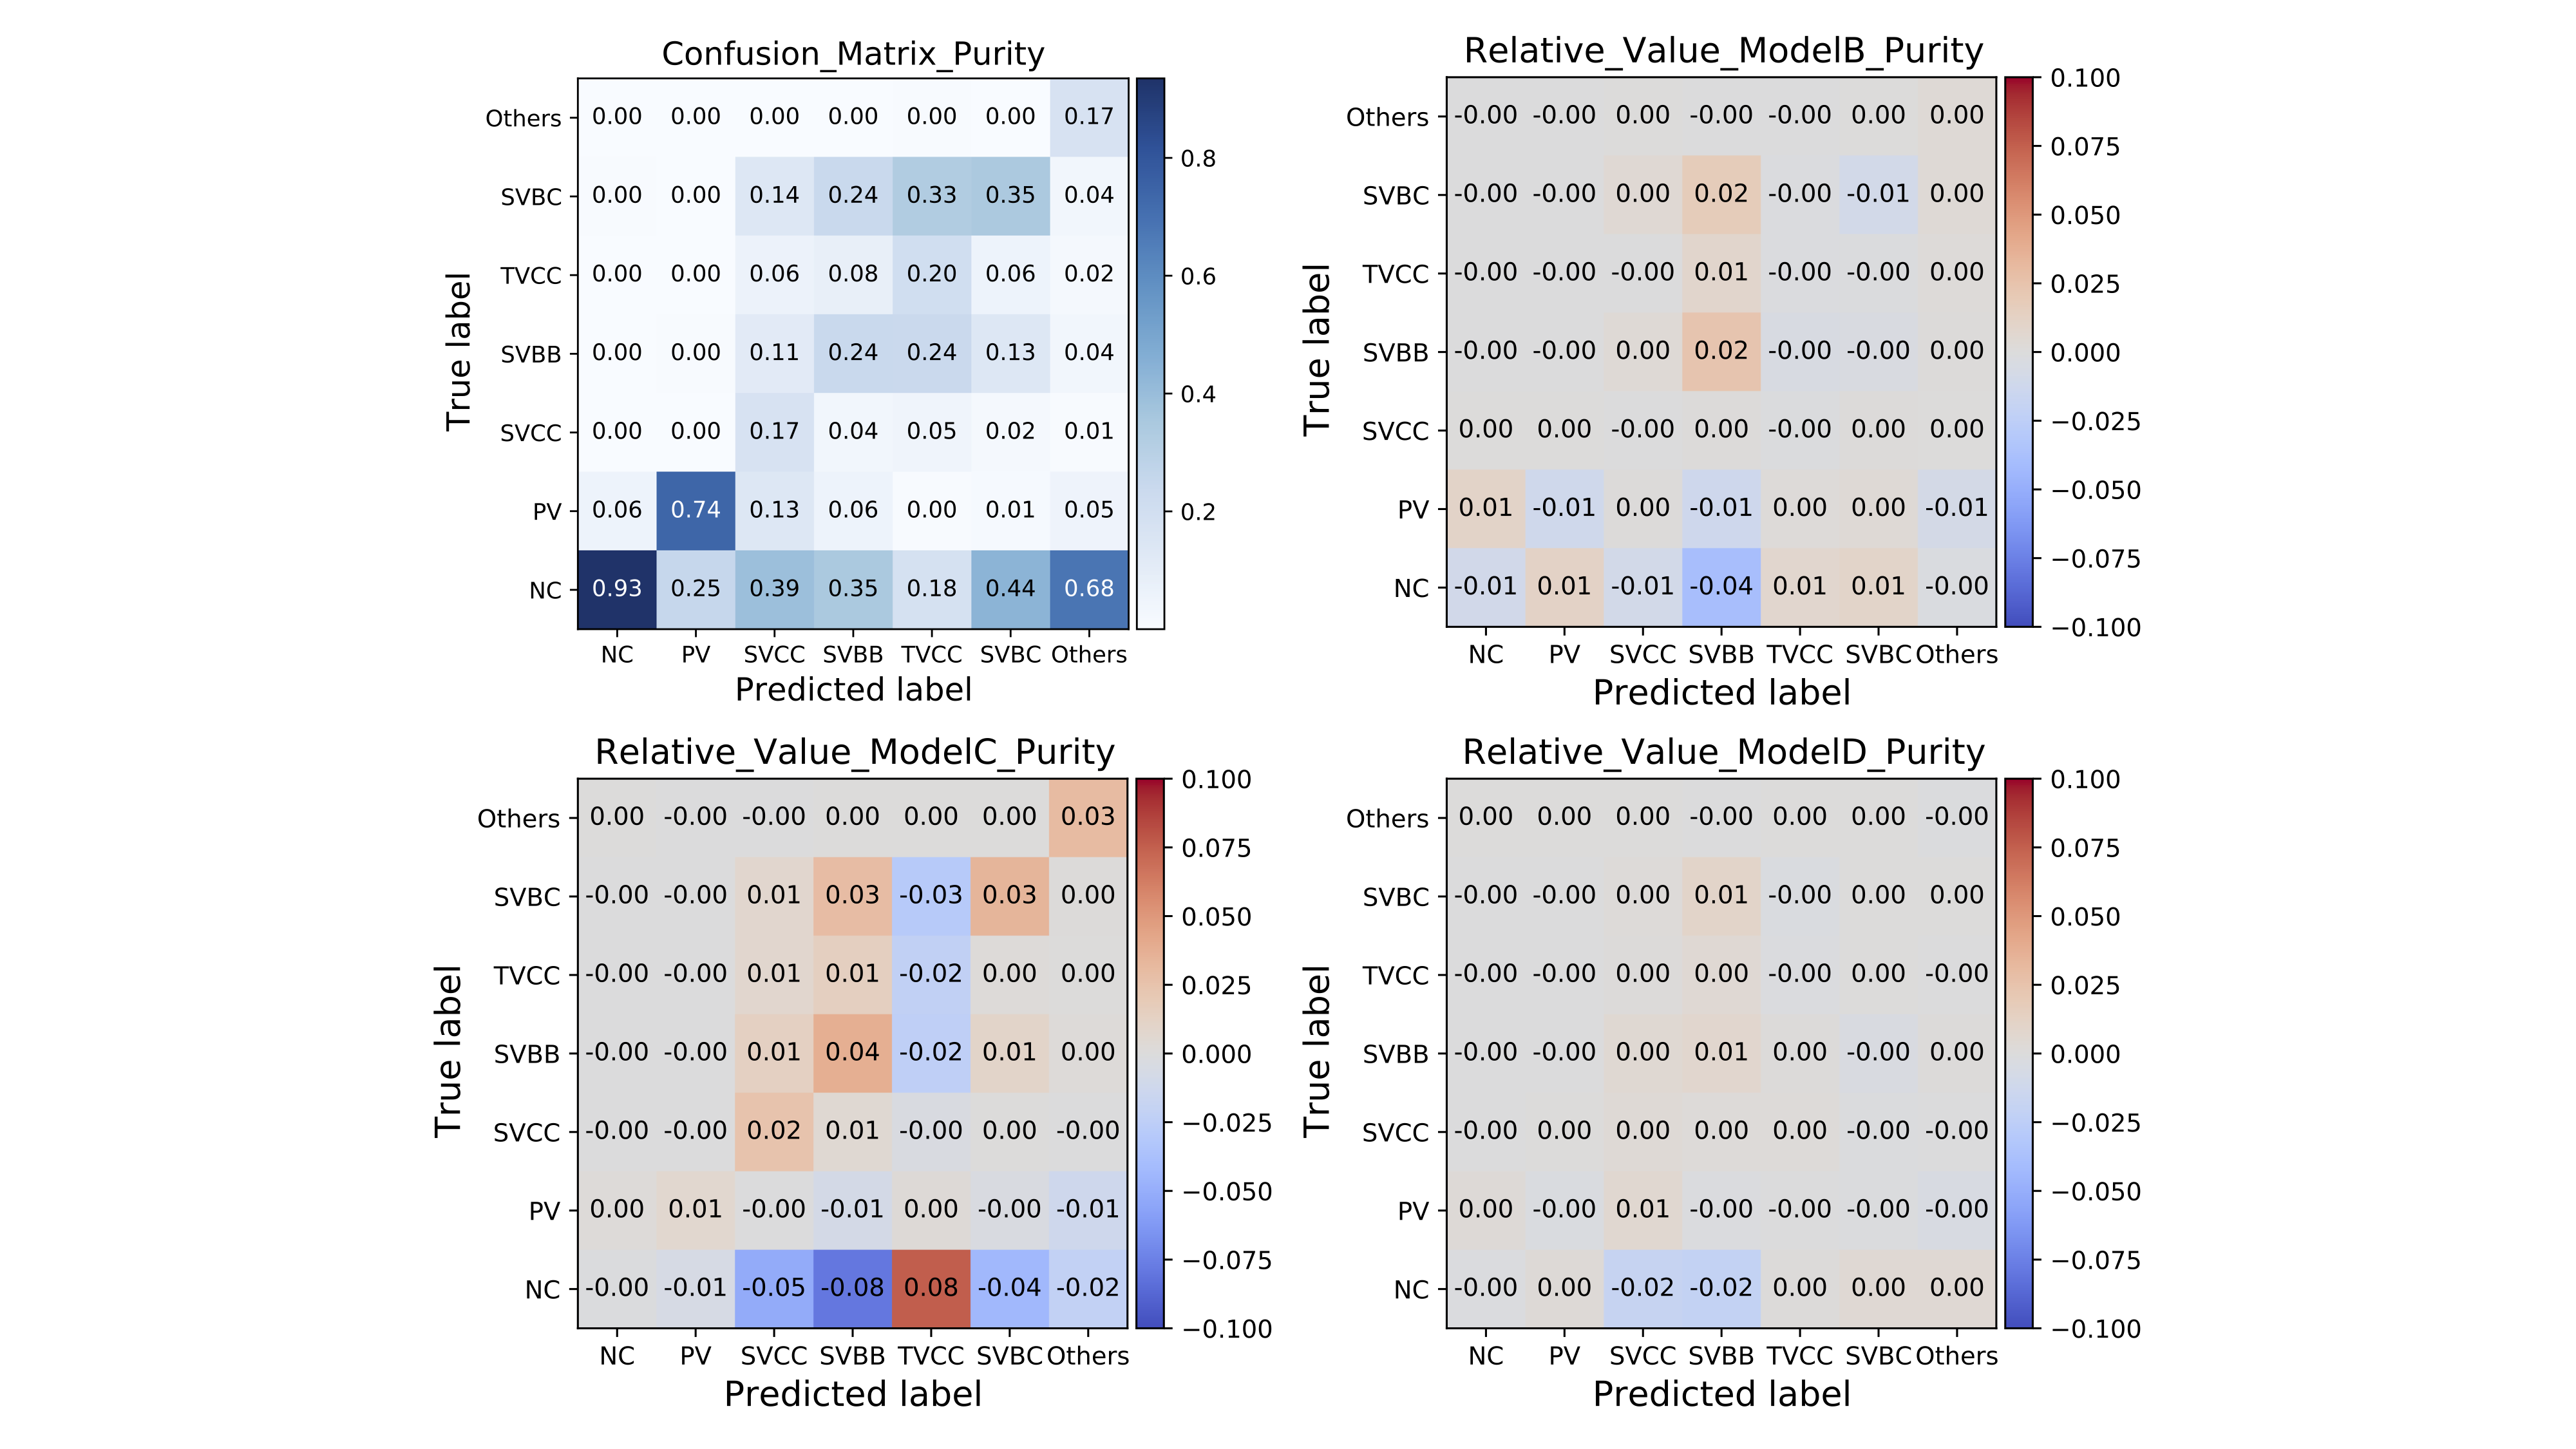
\includegraphics[trim = 300 0 300 0, width=0.9\textwidth, clip]{Figure/3Networks/3-3-3-2ConfusionMatrix_2.png}
   \end{minipage}
  \caption[各モデルの混合行列と各モデルの相対値]{各モデルの混合行列と各モデルの相対値。図上部は効率について規格化, 図下部は純度について規格化した行列である。それぞれ左上がモデルA, 右上がモデルB, 左下がモデルC, 右下がモデルDの結果である。モデルB・C・Dに関してはモデルAとの相対値で表現している。}
  \label{3-3-3-2ConfusionMatrix}
 %\end{tabular}
\end{figure}

図上部は効率について規格化したものである。
そのため正解ラベル方向 (行方向) の和が1になっている。
混合行列では, NP・PV・SVCC・Othersが比較的高い効率で分離できていることが分かる。
一方, 各SVについては殆ど分離できておらす, 個々のフレーバーや準崩壊点などは区別できていない。
ただし, SVとそれ以外との分離は実現できており, SVであることは識別できているが, それがSVのどの崩壊点の種類であるかという点については識別が不十分となっている。

図下部は純度について規格化したものである。
そのため予想されたクラス方向 (列方向) の和が1になっている。
純度については不均衡データとしての特性が強調され, 図\ref{3-3-2-2ImbalancedData}のようなNCやPVが支配的なクラス配分となっていることから, 各SVに対してのNCからの汚染が顕著である。
ただし, これは後述する\ref{VFDL:TuneandPerformanceofVFDL}節での崩壊点のタネの選別によってある程度の軽減が可能である。

相対値では対角成分が正であれば性能が高い, それ以外の成分が正であれば性能が低いと判断できる。
ModelA・B・Dについてはあまり変化はなく, 殆どの差異は$0$~$2$\%程度に収まっている。
ModelCについても同様に大きな違いは確認できないが, 効率について規格化した混合行列内のSVBB・TVCC・SVBCの分類性能が向上しており, かつ純度について規格化した混合行列内のNCからのSVCC・SVBB・SVBCへの流入がある程度減少している。
ここで, TVCCへの流入しついては大幅に増大しているが, これはTVCCへの他のSVからの流入が少なくなったことによって相対的に上昇している為であると考えられる。

以上のことから, ネットワークはNC・PV・Othersや単にSVとしては大まかにクラス分類ができていると分かる。
また, 位置に関してもある程度の予想ができていると考えられる(図\ref{})。
一方, SV内の各崩壊点の種類への分離は困難でありModelCで多少の改善が見られることから, 詳細な位置の再構成には至っておらず, SV内の分離に関しては更なる情報の入力, もしくは抜本的なネットワーク構造の改良が必要であると考えられる。\\

2. t-SNEによるネットワークの理解\\

深層学習のネットワーク内部を理解することは非常に難しい課題の一つである。
ネットワークが何故, どのようにクラス分類を決定したかを把握する事は容易ではないが, どの程度各クラスを分離して判断できているかは次元削減によってある程度理解が可能である。
ここでは, t-SNEという手法を用いて次元削減を行った。

t-SNEとは, 高次元の情報についての距離関係を維持しつつ, 低次元へマッピングするアルゴリズムである。
データの局所的な構造や非線形の次元削減が可能であり, ここではネットワークがどの程度各クラスを分離できているかを二次元の画像として把握することができる。

そのような結果を図\ref{3-3-3-3tSNE}に示す。
入力変数では殆ど分離できていなかった各クラスが, 出力層の直前ではある程度分離できている事が確認できる。
また, 各SVは非常に近い位置にマップされており, 分離が困難であると分かる。
更に, 分布は線対称な形をしており, これは二本の飛跡についての情報を十分に混合できていないということを意味していると考えられる。

\begin{figure}[htbp]
 \centering
 \includegraphics[width=1.0\textwidth]{Figure/3Networks/3-3-3-3tSNE.png}
 \caption[t-SNEによる次元削減の比較]{t-SNEによる次元削減の比較。左図は入力変数 ($22$変数) を二次元に削減したもの, 右図は分類問題への分離の直前の全結合層 ($256$変数) を二次元に削減したものである。}
 \label{3-3-3-3tSNE}
\end{figure}


%%%%%%%%%%%%%%%%%%%%%%%%%%%%%%%%%%%%%%%%%%%%%%%%%%%%%%%%%%%%%%%%%%%%%%%%%%%%%%%%%%%%%%%%%%%%%%%%%%%%%
\section{任意の数の飛跡についてのネットワーク} \label{Net:VertexLSTM}

ここでは\ref{Net:forVertexFinderwithDL}節で紹介した二つのネットワークの内, 任意の数の飛跡についてのネットワークに関して述べる。
前節と同様にネットワークの構造・学習・評価について\ref{Net:VLSTM:StructureofVLSTM}項・\ref{Net:VLSTM:TrainingandStrategyofVLSTM}項・\ref{Net:VLSTM:PerformanceofVLSTM}項でそれぞれ解説する。

任意の数の飛跡についてのネットワークは, 崩壊点を生成するためのネットワークである。
ここでは, リカレントニューラルネットワークの初期状態として飛跡対 (崩壊点のタネ) を入力し, 系列データとして事象中の全ての飛跡を入力する。
また出力の作り方はMany to Manyとし, 事象中のそれぞれの飛跡が初期状態の崩壊点のタネに対して結合しているか否かを評価するネットワークを構築する。

\begin{figure}[htbp]
 \centering
 \includegraphics[trim = 200 150 200 150, width=0.9\textwidth, clip]{Figure/3Networks/3-4-0-1VertexProductionwithRNN.png}
 \caption[リカレントニューラルネットワークを用いた崩壊点生成]{リカレントニューラルネットワークを用いた崩壊点生成。初期状態として崩壊点のタネを入力し, 系列データとして事象中の飛跡を入力している。事象中の飛跡はそれぞれ一本ずつ評価され, 出力はそれらの飛跡が初期状態の崩壊点のタネと結合しているか, 非結合であるかである。}
 \label{3-4-0-1VertexProductionwithRNN}
\end{figure}


%%%%%%%%%%%%%%%%%%%%%%%%%%%%%%%%%%%%%%%%%%%%%%%%%%%%%%%%%%%%%%%%%%%%%%%%
\subsection{ネットワークの構造} \label{Net:VLSTM:StructureofVLSTM}

まず, 任意の数の飛跡についてのネットワークとして図\ref{3-4-1-1SimpleVLSTM}のようなネットワークを考える。

\begin{figure}[htbp]
 \centering
 \includegraphics[trim = 100 200 100 200, width=1.0\textwidth, clip]{Figure/3Networks/3-4-1-1SimpleVLSTM.png}
 \caption[崩壊点生成のためのリカレントニューラルネットワーク構造]{崩壊点生成のためのリカレントニューラルネットワーク構造。図上部で崩壊点の生成の様子を図示した。飛跡がタネに結合していれば隠れ状態は逐次的に更新されていき, 事象中の全ての飛跡を評価した段階で崩壊点が生成される。実際には系列データとして入力される飛跡に関しても, 全結合層を用いてEmbeddingを行い抽象化している。}
 \label{3-4-1-1SimpleVLSTM}
\end{figure}

前述したように崩壊点のタネを初期状態として使用している。
実際には崩壊点のタネは飛跡二本分の情報 ($44$個の変数) であり, 更に全結合層を介してより抽象的な崩壊点の情報を初期状態として入力できるようにしている。
また系列データとして事象中の全ての飛跡を用いている。
出力はこの飛跡のそれぞれが崩壊点のタネと結合しているか否かである。

\ref{DL:RNN:LongShortTermMemory}で解説したようにリカレントニューラルネットワークは系列情報を保持する為, 直前の系列に依存するように設計されている。
しかし飛跡は本質的に順序を持っていないことに注意する必要がある。
図\ref{3-4-1-1SimpleVLSTM}では便宜的に飛跡について番号を振り表現しているが, これは人が決めた順序であり, 本来, 事象中の飛跡は系列データではない。
したがって, リカレントニューラルネットワークをそのまま用いることはデータの性質に合わない。
この為私は, リカレントニューラルネットワークの一つであるLSTMを拡張し, 新しい独自のリカレントニューラルネットワークの構造を構築した。

図\ref{3-4-1-2VLSTMStructure}はそのような独自のリカレントニューラルネットワークについての1系列分のステップの詳細である。

\begin{figure}[htbp]
 \centering
 \includegraphics[trim = 0 100 0 200, width=0.9\textwidth, clip]{Figure/3Networks/3-4-1-2VLSTMStructure.png}
 \caption[系列1ステップについての独自リカレントニューラルネットワーク構造]{系列1ステップについての独自リカレントニューラルネットワーク構造。図\ref{3-4-1-1SimpleVLSTM}の青丸の一つに相当している。}
 \label{3-4-1-2VLSTMStructure}
\end{figure}

LSTMとの大きな構造の違いは, 短期記憶である${\mbox{\boldmath{$h$}}}_t$が隠れ状態として入出力されていない点である。
入力は隠れ状態の記憶セル${\mbox{\boldmath{$c$}}}_{t-1}$と系列データ${\mbox{\boldmath{$x$}}}_t$の二つである。
また出力は結合・非結合を判定する${\mbox{\boldmath{$h$}}}_t$と隠れ状態の記憶セル${\mbox{\boldmath{$c$}}}_{t}$の二つである。
隠れ状態として${\mbox{\boldmath{$h$}}}_t$が使用されていないため, 内部の構造も通常のLSTMとは少し異なり, 出力${\mbox{\boldmath{$h$}}}_{t}$と記憶セル${\mbox{\boldmath{$c$}}}_{t}$はそれぞれ
\begin{equation}
 \begin{split}
  &{\mbox{\boldmath{$c$}}}_{t} 
  = (1-{\mbox{\boldmath{$h$}}}_t) {\mbox{\boldmath{$c$}}}_{t-1} + {\mbox{\boldmath{$h$}}}_t {\mbox{\boldmath{$c'$}}}_{t}\\
  &{\mbox{\boldmath{$c'$}}}_{t}
  = {\mbox{\boldmath{$c$}}}_{t-1} \  \sigma (W_f {\mbox{\boldmath{$x$}}}_t + R_f {\mbox{\boldmath{$c$}}}_{t-1}) 
  + \tanh (W_c {\mbox{\boldmath{$x$}}}_t + R_c {\mbox{\boldmath{$c$}}}_{t-1}) \  \sigma (W_i {\mbox{\boldmath{$x$}}}_t + R_i {\mbox{\boldmath{$c$}}}_{t-1})\\
  &{\mbox{\boldmath{$h$}}}_{t} 
  = \sigma (D_h [\tanh({\mbox{\boldmath{$c$}}}_{t-1}) \  \sigma (W_o {\mbox{\boldmath{$x$}}}_t + R_o {\mbox{\boldmath{$c$}}}_{t-1}) ])
 \end{split}
\end{equation}
となる。
第二式の${\mbox{\boldmath{$c'$}}}_{t}$は更新された記憶セルを示している。
第三式は出力ゲートに更に全結合層を掛けた形となっており, 二値分類の為の出力を作成している。
第一式では, 更新された記憶セル${\mbox{\boldmath{$c'$}}}_{t}$と直前の系列での記憶セル${\mbox{\boldmath{$c$}}}_{t-1}$, 出力${\mbox{\boldmath{$h$}}}_{t}$を用いて現在の記憶セル${\mbox{\boldmath{$c$}}}_{t}$を計算している。
二値分類であるので, ${\mbox{\boldmath{$h$}}}_{t}$は$0$から$1$の値を持つはずである。
したがって, 第一式は結合(${\mbox{\boldmath{$h$}}}_{t} \sim 1$)していれば更新された記憶セル${\mbox{\boldmath{$c'$}}}_{t}$が, 非結合(${\mbox{\boldmath{$h$}}}_{t} \sim 0$)であれば, 直前の系列での記憶セル${\mbox{\boldmath{$c$}}}_{t-1}$が現在の記憶セル${\mbox{\boldmath{$c$}}}_{t}$となることを示している。

初期状態は崩壊点のタネであるので, 以上の演算は次のように (図\ref{3-4-1-3Interpretation}) 解釈できる。

\begin{enumerate}
 \item $t-1$番目の崩壊点${\mbox{\boldmath{$c$}}}_{t-1}$と$t$番目の飛跡${\mbox{\boldmath{$x$}}}_{t}$が結合しているか否かの評価${\mbox{\boldmath{$h$}}}_{t}$を行う
 \item $t-1$番目の崩壊点${\mbox{\boldmath{$c$}}}_{t-1}$と$t$番目の飛跡${\mbox{\boldmath{$x$}}}_{t}$を用いて更新された崩壊点${\mbox{\boldmath{$c'$}}}_{t}$を計算する
 \item $t-1$番目の崩壊点${\mbox{\boldmath{$c$}}}_{t-1}$と$t$番目の飛跡${\mbox{\boldmath{$x$}}}_{t}$が結合しているならば更新された崩壊点${\mbox{\boldmath{$c'$}}}_{t}$を, 結合していないならば$t-1$番目の崩壊点${\mbox{\boldmath{$c$}}}_{t-1}$を$t$番目の崩壊点${\mbox{\boldmath{$c$}}}_{t}$として選択する
\end{enumerate}

\begin{figure}[htbp]
 \centering
 \includegraphics[width=0.9\textwidth, clip]{Figure/3Networks/3-4-1-3Interpretation.png}
 \caption[独自リカレントニューラルネットワーク構造の解釈]{独自リカレントニューラルネットワーク構造の解釈。それぞれの丸が演算に対応している。左下が演算1, 中央が演算2, 右上が演算3である。}
 \label{3-4-1-3Interpretation}
\end{figure}

短期記憶を破棄する事によって, 独自リカレントニューラルネットワークでは, 事象中の飛跡の順序 (短期記憶) にできる限り依存させず, 更に崩壊点のタネに対して飛跡を足していくことによって更新される崩壊点の情報 (記憶セル) を表現している。\\

私たちはシミュレーションデータとして既に一つの事象分の全ての飛跡についての情報を持っている。
したがって, 作成したリカレントニューラルネットワークをエンコーダー・デコーダーモデルに組み込むことで, 事象についての情報 (コンテキスト) を活用することができると考えられる。
また, エンコーダー・デコーダーモデルの間にAttentionを組み込むことも同様に自然な発想である。
その様なネットワークを図\ref{3-4-1-4EncoderDecoderVLSTM}に示す。

\begin{figure}[htbp]
 \centering
 \includegraphics[trim = 100 200 100 100, width=1.0\textwidth, clip]{Figure/3Networks/3-4-1-4EncoderDecoderVLSTM.png}
 \caption[Attentionを組み込んだエンコーダー・デコーダーモデルへの拡張]{Attentionを組み込んだエンコーダー・デコーダーモデルへの拡張。図上部がエンコーダー部, 図下部がデコーダー部をそれぞれ示している。初期状態や系列データはエンコーダー部とデコーダー部のそれぞれに入力されている。エンコーダー部では双方向RNNを用いている。ただし, ここのステップは独自構造のネットワークになっている。エンコーダー部の出力は図中央のKey・Valueに集められ, デコーダー部に入力される。デコーダー部での出力はそれぞれの飛跡がタネと結合しているか, 非結合であるかの二値分類である。}
 \label{3-4-1-4EncoderDecoderVLSTM}
\end{figure}

図の上部はエンコーダー部である。
エンコーダー部では事象中の飛跡から事象全体の情報 (コンテキスト) を抽出している。
ここでは先ほどの図\ref{3-4-1-1SimpleVLSTM}で紹介したネットワークを双方向リカレントニューラルネットワークとして使用している。
ただし, 出力${\mbox{\boldmath{$h$}}}_{t}$の次元数を減らさないようにするため全結合層$D_h$を取り除いている。
また図中で表現しているように, 双方向から入力されている崩壊点のタネはそれぞれ別の全結合層によって情報を抽象化されている。

図の下部はデコーダー部である。
デコーダー部ではエンコーダー部で抽出された情報と崩壊点のタネ, 事象中の飛跡を使用して崩壊点のタネにそれぞれの飛跡が結合しているか否かを判別している。
エンコーダー部で抽出された情報はAttentionによって適切に評価され, デコーダー部の"ある"飛跡がエンコーダー部の任意の飛跡に対して注意を払って, 事象中の情報を取得できるようになっている。
またエンコーダー・デコーダーモデルへの拡張後も, このネットワークの基本構造がリカレントニューラルネットワークであることに変わりはない為, 飛跡の本数を任意に変えることが可能である。

図\ref{3-4-1-2VLSTMStructure}で示したネットワーク構造はAttentionには対応していないため, 新たなネットワークの構築が必要である。
そのようなネットワークを図\ref{3-4-1-5AttentionVLSTM}に示す。

\begin{figure}[htbp]
 \centering
 \includegraphics[trim = 100 0 100 0, width=0.9\textwidth, clip]{Figure/3Networks/3-4-1-5AttentionVLSTM.png}
 \caption[独自リカレントニューラルネットワークのAttentionへの拡張]{独自リカレントニューラルネットワークのAttentionへの拡張。図\ref{3-4-1-4EncoderDecoderVLSTM}の赤丸の一つに相当している。図上部の青線は不変記憶Key・Valueの流れを表している。Attentionに関する演算が加えられている点以外は図\ref{3-4-1-2VLSTMStructure}と同様の構造である。}
 \label{3-4-1-5AttentionVLSTM}
\end{figure}

本研究では, エンコーダー部で抽出された情報 (Key) をリカレントニューラルネットワークの隠れ状態の一つとして入力している。
また, このKeyはネットワークの各ステップについて共通の値を使用しており, 長期記憶・短期記憶と比べて不変記憶のような役割を果たしている。
Attention Weightの計算方法としてAdditive Attentionを採用した。
$t$番目のコンテキスト${\mbox{\boldmath{$\gamma$}}}_{t}$は次のように計算される。
\begin{equation}
 \begin{split}
  {\mbox{\boldmath{$\gamma$}}}_{t} 
  &= {\mbox{\boldmath{$\alpha$}}}_{t} V\\
  {\mbox{\boldmath{$\alpha$}}}_{t}
  &= (\alpha_{t,0},\ \alpha_{t,1},\ \alpha_{t,2},\ \cdots \alpha_{t,i},\ \cdots) \\
  &= \left(\frac{\exp{({{e}}_{t,0})}}{\sum_j \exp{({{e}}_{t,j})}},\ \frac{\exp{({{e}}_{t,1})}}{\sum_j \exp{({{e}}_{t,j})}},\ \frac{\exp{({{e}}_{t,2})}}{\sum_j \exp{({{e}}_{t,j})}},\  \cdots \frac{\exp{({{e}}_{t,i})}}{\sum_j \exp{({{e}}_{t,j})}},\ \cdots\right)\\
  {\mbox{\boldmath{$e$}}}_{t}
  &={\mbox{\boldmath{$u$}}}_{\rm energy} (K\ U_{\rm key} + X_t\ U_{\rm query}) \\
 \end{split}
\end{equation}
ここで, Keyを$K$, Valueを$V$, $t$番目のQueryである飛跡${\mbox{\boldmath{$x$}}}_{t}$を重ねた行列を$X_t$, $t$番目のAttention Weightを${\mbox{\boldmath{$\alpha$}}}_{t}$, $t$番目のQueryについてのエネルギーを${\mbox{\boldmath{$e$}}}_{t}$とした。
また, Additive Attentionにおける重み行列をそれぞれ${\mbox{\boldmath{$u$}}}_{\rm energy},\  U_{\rm key},\ U_{\rm query}$と置いた。

添字$i,\ j$はエンコーダー部の系列, 添字$t$はデコーダー部の系列である。
したがって$t$番目のAttention Weight${\mbox{\boldmath{$\alpha$}}}_{t}$はエンコーダー部の飛跡の数だけ要素を持っており, デコーダー部の全ての飛跡についてAttention Weightを計算した時, Attention Weightはエンコーダー部の飛跡の数$\times$デコーダー部の飛跡の数の行列となる。
このAttention Weight行列はネットワーク内部を把握する上で非常に重要な情報である。
図\ref{3-4-1-5AttentionVLSTM}では表現していないがオプションとしてAttention Weightを出力することで, ネットワーク内部をある程度理解することができる。

得られた$t$番目のコンテキスト${\mbox{\boldmath{$\gamma$}}}_{t}$は, 出力${\mbox{\boldmath{$h$}}}_{t}$や更新された崩壊点${\mbox{\boldmath{$c'$}}}_{t}$の計算に使用される。
\begin{equation}
 \begin{split}
  &{\mbox{\boldmath{$c$}}}_{t} 
  = (1-{\mbox{\boldmath{$h$}}}_t) {\mbox{\boldmath{$c$}}}_{t-1} + {\mbox{\boldmath{$h$}}}_t {\mbox{\boldmath{$c'$}}}_{t}\\
  &{\mbox{\boldmath{$c'$}}}_{t}
  = {\mbox{\boldmath{$c$}}}_{t-1} \  \sigma (W_f {\mbox{\boldmath{$x$}}}_t + R_f {\mbox{\boldmath{$c$}}}_{t-1} + C_f {\mbox{\boldmath{$\gamma$}}}_{t})\\
  &+ \tanh (W_c {\mbox{\boldmath{$x$}}}_t + R_c {\mbox{\boldmath{$c$}}}_{t-1} + C_c {\mbox{\boldmath{$\gamma$}}}_{t}) \  \sigma (W_i {\mbox{\boldmath{$x$}}}_t + R_i {\mbox{\boldmath{$c$}}}_{t-1} + C_i {\mbox{\boldmath{$\gamma$}}}_{t})\\
  &{\mbox{\boldmath{$h$}}}_{t} 
  = \sigma (D_h [\tanh({\mbox{\boldmath{$c$}}}_{t-1}) \  \sigma (W_o {\mbox{\boldmath{$x$}}}_t + R_o {\mbox{\boldmath{$c$}}}_{t-1} + C_o {\mbox{\boldmath{$\gamma$}}}_{t}) ])
 \end{split}
\end{equation}
式中ではコンテキスト${\mbox{\boldmath{$\gamma$}}}_{t}$に関する各ゲートそれぞれの重み行列を$C_f,\ C_c,\ C_i,\ C_o$と置いた。
$t$番目のコンテキスト${\mbox{\boldmath{$\gamma$}}}_{t}$についての演算を加えている点以外は図\ref{3-4-1-2VLSTMStructure}でのネットワークの演算と全く同様である。


%%%%%%%%%%%%%%%%%%%%%%%%%%%%%%%%%%%%%%%%%%%%%%%%%%%%%%%%%%%%%%%%%%%%%%%%
\subsection{ネットワークの学習と戦略} \label{Net:VLSTM:TrainingandStrategyofVLSTM}

訓練データとして必要な情報は, 初期状態としての飛跡対 (崩壊点のタネ) と事象中の全ての飛跡である。
また, 正解ラベルはそれぞれの飛跡が崩壊点のタネと結合しているか否かのMC情報である。
推論時は, 初期状態の崩壊点のタネとして非結合な飛跡対が入力される場合が考えられるが, 本研究ではネットワークの学習時は崩壊点のタネとして結合している飛跡対 (PV・SVCC・SVBB・TVCC) のみを使用する。
ここで, 準崩壊点SVBCは崩壊点生成において雑音となりうる可能性があるため含んでいない。

リカレントニューラルネットワークでは, 推論時は系列長を変えることができるが, 学習時は重み更新の計算のため系列長を揃える必要がある。\footnote{実際にはバッチサイズ毎に}
ここでの系列長は事象中の飛跡の本数であった。
このため, 不足している飛跡の本数をゼロ埋め (Zero padding) し, ゼロ埋めした飛跡が学習に影響しないよう損失関数においてマスクしている。
本研究では最も飛跡数の多い事象との兼ね合いから系列長を$60$本とし, それ以下の本数の事象については$60$本となるようにゼロ埋めしている。

最終的な入力変数の大きさを表\ref{VLSTMInputParameterShape}に示す。

\begin{table}[htb]
 \centering
 \small
  \begin{tabular}{c | c c}\hline
    & PV & SV\\\hline
    崩壊点のタネ & $(1661307,\ 44)$ & $(367434,\ 44)$\\
    事象中の全ての飛跡 & $(1661307,\ 60,\ 23)$ & $(367434,\ 60,\ 23)$\\\hline
  \end{tabular}
  \caption{任意の数の飛跡についてのネットワークの入力変数の大きさ}
  \label{VLSTMInputParameterShape}
\end{table}

ここで, 第一引数はデータのサンプル数である。
訓練データは全ての崩壊点のタネについて一つのサンプルが生成されるため, 全ての事象 ($\rm c\bar{c}-05,\ \rm b\bar{b}-06$) を使用すると非常に時間がかかる。
よって, 本研究では全ての事象を使用して訓練データを作成した後, 1エポック毎にランダムに$50000$サンプルを訓練に$10000$サンプルを検証に使用している。
事象中の全ての飛跡については飛跡の本数である$60$本とそれぞれの飛跡について$22$個の変数を持っている。
また, ゼロ埋めした飛跡との区別のためのマスク変数 $(0,\ 1)$ を一つ加えている。

崩壊点生成において, 飛跡は順序を持って足されていく。
短期的な順序に依存しないような独自のネットワークを構築しているが, そのような人によって決められた飛跡の順序にネットワークが依存してしまうことは, できる限り避けねばならないため, 1エポック毎に飛跡の系列順をランダムにシャッフルしている。

\begin{figure}[htbp]
 \centering
 \includegraphics[trim = 150 100 150 100, width=0.9\textwidth, clip]{Figure/3Networks/3-4-2-1TrackShuffle.png}
 \caption[飛跡順のシャッフル]{飛跡順のシャッフル。$1$エポック毎に系列データの飛跡順序をシャッフルし, 崩壊点のタネへ足し合わせる順番への依存を取り除いた。この順序のシャッフルは学習や検証に使用する全てのデータについて同一である。}
 \label{3-4-2-1TrackShuffle}
\end{figure}

損失関数は二値交差エントロピー誤差を使用した。
ただし, 前述したようにゼロ埋めした飛跡については損失関数や正答率の計算ではマスクした。
\begin{equation}
 \begin{split}
 L = -M_{\rm ZP}\ t_{\rm C} \log{(y_{\rm C})} - M_{\rm ZP}\ (1-t_{\rm C})\ \log{(1-y_{\rm C})}
 \end{split}
\end{equation}
$M_{\rm ZP}$はゼロ埋めのためのマスク変数 $(0,\ 1)$ である。

ハイパーパラメータとして, 最適化手法はAdam, 学習率は$0.001$, エポック数は$100$, バッチサイズは$32$を用いた。
また, ネットワークの学習可能な重みのパラメータ数を表\ref{ParametersforVLSTMModel}に示す。

\begin{table}[htb]
 \centering
 \small
 \scalebox{0.8}{
  \begin{tabular*}{1.2\textwidth}{@{\extracolsep{\fill}}l c c l}\hline
    層の名称 & 出力の形状 & パラメータ数 & 接続先\\\hline\hline
    Pair Input & (None, 44) & 0 & \\\hline
    Encoder Input & (None, 60, 23) & 0 \\\hline
    Decoder Input & (None, None, 23) & 0 \\\hline\hline
    Encoder Forward Dense 1 & (None, 256) & 11520 & Pair Input\\\hline
    Encoder Backward Dense 1 & (None, 256) & 11520 & Pair Input\\\hline
    Encoder Forward Activation 1 & (None, 256) & 0 & Encoder Forward Dense 1\\\hline
    Encoder Backward Activation 1 & (None, 256) & 0 & Encoder Backward Dense 1\\\hline
    Encoder Forward Dense 2 & (None, 256) & 11520 & Encoder Forward Activation 1\\\hline
    Encoder Backward Dense 2 & (None, 256) & 11520 & Encoder Backward Activation 1\\\hline
    Encoder Forward Activation 2 & (None, 256) & 0 & Encoder Forward Dense 2\\\hline
    Encoder Backward Activation 2 & (None, 256) & 0 & Encoder Backward Dense 2\\\hline\hline
    Encoder Embedding Dense & (None, 60, 256) & 6144 & Encoder Input\\\hline\hline
    Bidirectional Encoder VLSTM & (None, 60, 512) & 1050624 & Encoder Embedding Dense\\     
                                                                                                         &&&Encoder Forward Activation 2\\       
                                                                                                         &&&Encoder Forward Activation 2\\       
                                                                                                         &&&Encoder Backward Activation 2\\     
                                                                                                         &&&Encoder Backward Activation 2\\ \hline
    Reshape Bidirectional Encoder & (None, 27136) & 0 & Bidirectional Encoder VLSTM\\\hline\hline
    Decoder Dense 1 & (None, 256) & 11520 & Pair Input\\\hline
    Decoder Activation 1 & (None, 256) & 0 & Decoder Forward Dense 1\\\hline
    Decoder Dense 2 & (None, 256) & 11520 & Decoder Forward Activation 1\\\hline
    Decoder Activation 2 & (None, 256) & 0 & Decoder Forward Dense 2\\\hline\hline
    Decoder Embedding Dense & (None, None, 256) & 6144 & Encoder Input\\\hline\hline
    Decoder Attention VLSTM & (None, None, 1) & 1246976 & Decoder Embedding Dense\\
                                                                                                   &&& Reshape Bidirectional Encoder\\                    
                                                                                                   &&& Decoder Activation 2\\\hline\hline
  \end{tabular*}
  }
  \caption{任意の数の飛跡についてのネットワークにおける訓練可能なパラメータ}
  \label{ParametersforVLSTMModel}
\end{table}


%%%%%%%%%%%%%%%%%%%%%%%%%%%%%%%%%%%%%%%%%%%%%%%%%%%%%%%%%%%%%%%%%%%%%%%%
\subsection{ネットワークの評価} \label{Net:VLSTM:PerformanceofVLSTM}

ネットワークの評価は飛跡対についてのネットワークと同様に, 1. ネットワーク間の比較と2. ネットワーク内の理解の二つの観点で行う。
任意の数の飛跡についてのネットワークでは, 1. ネットワーク間の比較については標準的なLSTMと本研究で構築した独自のネットワークの比較を行う。
更に, 終状態の違いや崩壊点のタネの違いについて, 各データ属性に特化したネットワークとそれら全てのデータを用いて学習した標準的なネットワークについての比較を行う。
2. ネットワーク内の理解については任意の数の飛跡についてのネットワークは内部にAttentionを持っているため, Attention Weightを確認することにより, エンコーダー部からどのような情報を抽出しているかについて調査する。\\

1. ネットワーク間の比較\\

まず, 以下の三つのネットワークの比較によって独自のネットワーク構造がどの程度効果的であるかの確認を行う。

\begin{itemize}
 \item 標準的なLSTM : 図\ref{3-4-1-1SimpleVLSTM}のようなネットワークの個々のステップを標準的なLSTMに置き換えたネットワーク
 \item 独自のLSTM : 図\ref{3-4-1-1SimpleVLSTM}のようなネットワーク
 \item 独自のAttention LSTM : 図\ref{3-4-1-4EncoderDecoderVLSTM}のようなネットワーク
\end{itemize}

これらのネットワークに関して損失と正答率のエポック毎の変化を図\ref{3-4-3-1LSTMvsVLSTM}に示す。
ここでは全ての評価基準についてゼロ埋めした飛跡を取り除いている。
また, ネットワークの構造やデータ特性を考慮し, 正答率や真陽性率 (True Positive Rate, TPR), 真陰性率 (True Negative Rate, TNR) から初期状態となる飛跡対を取り除いている。

\begin{figure}[htbp]
 \centering
 \includegraphics[trim = 100 0 100 0, width=1.0\textwidth, clip]{Figure/3Networks/3-4-3-1LSTMvsVLSTM.png}
 \caption[標準的なLSTMと独自のネットワークの比較]{標準的なLSTMと独自のネットワークの比較。左上が損失, 右上が正答率, 左下がTPR, 右下がTNRである。それぞれ青線は標準的なLSTM, 赤線は独自のLSTM, 黒線は独自のAttention LSTMについての結果を表している。}
 \label{3-4-3-1LSTMvsVLSTM}
\end{figure}

標準的なLSTMは系列の順序を重視しているため学習が安定していないことが分かる。
また, 独自のネットワーク同士の比較においても, エンコーダー部からのコンテキストを受け取ることのできる独自のAttention LSTMの性能が高くなっている。
以上のことから, 標準的なLSTMを単純に使うことは不適であり, 独自のネットワーク構造による大幅な性能の改善が可能であると確認できる。\\

次に独自のAttention LSTMについての比較を行う。
ここでは訓練データをデータ属性毎に分離した。
ここでデータ属性とは終状態 ($\rm c\bar{c}$・$\rm b\bar{b}$) , 崩壊点のタネ (primary vertex (PV) ・secondary vertex (SV)) の4つである。
それぞれデータ属性のみで構成された訓練データで学習した特化型のネットワークを用意した。
それらのネットワークと全てのデータを使用した標準的なネットワークについての比較の結果を図\ref{3-4-3-2EfficiencyCurve}と図\ref{3-4-3-2ROCCurve}に示す。

\begin{itemize}
 \item ALL : 全てのデータを使用した標準的なネットワーク
 \item CC, BB : 終状態が$\rm c\bar{c}$, $\rm b\bar{b}$のデータのみを使用した特化型のネットワーク
 \item PV, SV : 崩壊点のタネがprimary vertex, secondary vertexのデータのみを使用した特化型のネットワーク
\end{itemize}

\begin{figure}[htbp]
 \centering
 \includegraphics[width=1.0\textwidth, clip]{Figure/3Networks/3-4-3-2EfficiencyCurve.png}
 \caption[各データ属性の効率とスコアの関係]{各データ属性の効率とスコアの関係。縦軸は効率, 横軸はネットワークのスコアについての閾値である。実線は信号効率, 破線はバックグラウンド効率である。黒線は全データを使用した標準的なネットワーク, 青線は個々の特化型のネットワークをそれぞれ表している。}
 \label{3-4-3-2EfficiencyCurve}
\end{figure}

\begin{figure}[htbp]
 \centering
 \includegraphics[width=1.0\textwidth, clip]{Figure/3Networks/3-4-3-2ROCCurve.png}
 \caption[各データ属性のROC曲線]{各データ属性のROC曲線。縦軸は信号効率, 横軸はバックグラウンド効率である。黒線は全データを使用した標準的なネットワーク, 青線は個々の特化型のネットワークをそれぞれ表している。}
 \label{3-4-3-2ROCCurve}
\end{figure}

比較に関してはROC曲線を使用している。
評価に際してのデータは特化型のネットワークの学習に使用した訓練データと同じ属性のものを用いた。
終状態$\rm c\bar{c}$や終状態$\rm b\bar{b}$に関しては基本的な性能の差がほとんどないと分かる。
したがって, 個々の終状態のデータに関してはその特性に大きな差異は存在しないと判断できる。
各崩壊点のタネに特化したネットワークに関しては両者とも性能の向上が見られた。
特に, PVのタネに特化したネットワークは結合と非結合との分離が非常に良くできている。
ROC曲線ではSVに特化したネットワークが標準的なネットワークより大幅に性能が改善されていると分かる。\\

2. ネットワーク内の理解\\

飛跡対についてのネットワークとは異なり, 任意の数の飛跡についてのネットワークはAttentionを持っている。
したがって, ネットワークの内部をAttention Weightを確認することによって, ネットワーク内部を把握することができる。
具体的には, エンコーダー部の飛跡がデコーダー部のどのような飛跡に注意し情報を受け取っているかを確認することが可能である。
そのようなAttention Weightについて, 標準的なネットワークとPVのタネを用いて作成したサンプルを図\ref{3-4-3-3AttentionWeight}に示す。

図上部は横軸がデコーダー部の飛跡番号, 縦軸がエンコーダー部の飛跡番号となっている。
ここではAttention Weightはカラースケールで表されている。
デコーダー部の飛跡によるAttention Weightの出力を縦方向に積んだような表現方法である。

図下部はエンコーダー部の飛跡を上に, デコーダー部の飛跡を下に並べた図となっている。
ここではAttention Weightは透過度で表現されている。
また, デコーダー部の飛跡の内, 崩壊点のタネと結合しているものを赤, 結合していないものを青で描画している。
デコーダー部の飛跡の数が少ないのはゼロ埋めを取り除いている為である。

これらの図から結合している飛跡はエンコーダー部の飛跡に注意し, 結合していない飛跡はエンコーダー部のゼロ埋めに注意している傾向があると分かる。

\begin{figure}[htbp]
 \centering
  %\begin{tabular}{cccc}
   \begin{minipage}{1.0\textwidth}
    \centering
    \includegraphics[trim = 200 0 200 0, width=1.0\textwidth, clip]{Figure/3Networks/3-4-3-3AttentionWeightMap.png}
    %\subcaption{終状態$\rm c\bar{c}$に特化したネットワーク}
    %\label{3-4-3-3AttentionWeightMap}
   \end{minipage}
   
   \begin{minipage}{1.0\textwidth}
   \centering
    \includegraphics[trim = 100 0 100 0, width=1.0\textwidth, clip]{Figure/3Networks/3-4-3-3AttentionWeightGraph.png}
    %\subcaption{終状態$\rm b\bar{b}$に特化したネットワーク}
    %\label{3-4-3-3AttentionWeightGraph}
   \end{minipage}
  \caption[Attention Weight]{図上部はAttention Weightを行列として表現した図, 図下部はAttention Weightをより直感的に示した図である。図上部では縦軸がデコーダーの飛跡番号, 横軸がエンコーダーの飛跡番号となっている。また, カラースケールはAttention Weightである。図下部では上段にデコーダーの飛跡, 下段にデコーダーの飛跡を描画している。デコーダーの飛跡ではタネと結合している飛跡については赤丸を使用している。}
  \label{3-4-3-3AttentionWeight}
 %\end{tabular}
\end{figure}




























% !TEX root = ../MasterThesis_goto_v1.tex

%%%%%%%%%%%%%%%%%%%%%%%%%%%%%%%%%%%%%%%%%%%%%%%%%%%%%%%%%%%%%%%%%%%%%%%%%%%%%%%%%%%%%%%%%%%%%%%%%%%%%
\chapter{深層学習を用いた崩壊点検出} \label{chap:VertexFinderwithDL}

本章では, 深層学習を用いた崩壊点検出について述べる。
前章では崩壊点検出のためのネットワークとして, 「1. 飛跡対についてのネットワーク」, 「2. 任意の数の飛跡についてのネットワーク」の二つのネットワークを導入した。
しかし, これら個々のネットワーク単体では崩壊点検出を実現できないため, これらを組み合わせたアルゴリズムが必要である。
そのようなアルゴリズムや前章までのネットワークについての総括を\ref{VFDL:AlgorithmofVFDL}節で行う。
また, このアルゴリズムではネットワークの出力に対する閾値などの幾つかのパラメータが必要なため, \ref{VFDL:TuneandPerformanceofVFDL}節では, それらパラメータの最適化について議論する。
同時に, どのような評価基準を用いて崩壊点検出の性能を判断するかについても, ここで述べる。
最後に\ref{VFDL:SummaryofVFDL}節では, 以上によって実現された崩壊点検出について改めて性能の評価をまとめる。


%%%%%%%%%%%%%%%%%%%%%%%%%%%%%%%%%%%%%%%%%%%%%%%%%%%%%%%%%%%%%%%%%%%%%%%%%%%%%%%%%%%%%%%%%%%%%%%%%%%%%
\section{崩壊点検出アルゴリズム} \label{VFDL:AlgorithmofVFDL}

前章では個々のネットワークについて, ネットワーク間の比較やネットワーク内の評価を行い単体での性能について理解を深めた。
「飛跡対についてのネットワーク」では, SVCC・SVBB・TVCC・SVBCの分離は非常に困難であり, 崩壊点のタネの段階での個々のsecondary vertexの識別は現実的ではないということがわかった。
「任意の数の飛跡についてのネットワーク」では, 個々の崩壊点の種類 (primary vertex・secondary vertex) に特化したネットワークの性能が標準的なネットワークの性能よりも僅かながら高いということを示した。
以上のことから, 本研究では崩壊点のタネをprimary vertexとsecondary vertexに分け, それぞれについて崩壊点の生成を行うこととした。

図\ref{3-3-2-2ImbalancedData}で示したように飛跡対の全ての組み合わせを考えた場合, そのクラスの比率はNCやPVが支配的なデータとなる。
よって, 図\ref{3-3-3-2ConfusionMatrix}のようにNCからの汚染により, SVCC・SVBB・TVCC・SVBCが埋もれてしまうという課題があった。
このようなNCは, データの構成からほとんどがprimary vertexとsecondary vertexから一本ずつ選ばれた飛跡で構成されていると考えられる。
したがって, この様な汚染はprimary vertexの再構成を精度よく行う事によって大幅に削減することが可能である。
また, 一般に事象中においてprimary vertexは必ず一つであり, かつprimary vertex由来の飛跡の数はその他の崩壊点と比べて多いため, primary vertexから再構成する方が妥当である。
これらのことを踏まえ, 図\ref{4-1-0-1VertexFinderAlgorithm}のような崩壊点検出アルゴリズムを提案する。
ここで, 「飛跡対についてのネットワーク」として表\ref{EvalationModels}で示したモデルAを用いる。
また, 「任意の数の飛跡についてのネットワーク」として\ref{Net:VLSTM:PerformanceofVLSTM}項で示したprimary vertexやsecondary vertexに特化したネットワークをそれぞれの崩壊点の生成に用いる。

\begin{figure}[htbp]
 \centering
 \includegraphics[width=0.9\textwidth, clip]{Figure/4VertexFinderwithDL/4-1-0-1VertexFinderAlgorithm.png}
 \caption{崩壊点検出アルゴリズム}
 \label{4-1-0-1VertexFinderAlgorithm}
\end{figure}

アルゴリズムは以下の手順で崩壊点の再構成を行う。

\begin{enumerate}
 \item 全事象から1事象分のデータを取り出し, 飛跡対の全ての組み合わせを考える。
 \item それら飛跡対に対して, 「飛跡対についてのネットワーク」を使用し, 崩壊点のタネの探索を行う。
 \item SVCC・SVBB・TVCC・SVBCと判定された飛跡対について, 選別を行いsecondary vertexのタネ (SVのタネ) を選ぶ。
 \item PVと判定されたタネ (PVのタネ) について, 「任意の数の飛跡についてのネットワーク」を用いprimary vertexの生成を行う。
 \item SVのタネとprimary vertex由来と判定された飛跡の情報を用い, 「任意の数の飛跡についてのネットワーク」によってSVのタネが無くなるまでsecondary vertexを生成する。
\end{enumerate}

手順1, 2については飛跡対についてのネットワークの訓練データの作成や学習と全く同様の手順である。

手順3では, 「飛跡対についてのネットワーク」によって得られるSVCC・SVBB・TVCC・SVBCのスコアや崩壊点の位置を用いてより純度の高いSVのタネの集合を作成する。
したがって, SVCC・SVBB・TVCC・SVBCのスコアについての閾値や崩壊点の位置についての最適化が必要である。

手順4では, 「飛跡対についてのネットワーク」によって得られるPVのスコアについて降順に並び替えたPVのタネの集合と「任意の数の飛跡についてのネットワーク」を用いてprimary vertexを生成する。
ここでは, PVのタネをスコアの高い方から幾つ用いるかについて最適化が必要である。
また一度以上, 「任意の数の飛跡についてのネットワーク」によって結合していると判定された飛跡をprimary vertex由来であると判断している。
この時の「任意の数の飛跡についてのネットワーク」によって得られる崩壊点のタネと結合しているかに関するスコアについての閾値についても, また同様に最適化が必要なパラメータである。

手順5について, 手順3で選別したSVのタネと手順4で得られたprimary vertex由来であると判定された飛跡の一覧を用いてsecondary vertexの再構成を行う。
ここでは「任意の数の飛跡についてのネットワーク」のデコーダー部に入力する飛跡から, 再構成されたsecondary vertex由来の飛跡を取り除いて行くことによって, 再帰的にsecondary vertexの生成が行われる。
初期状態として使用するSVのタネは, 飛跡対に含まれる飛跡がprimary vertex由来の飛跡の一覧や, それまでに生成したsecondary vertex由来の飛跡の一覧に存在していた場合は除外し, 次のSVのタネへ移行している。
このsecondary vertexに関する「任意の数の飛跡についてのネットワーク」のスコアも最適化が必要である。
また, 再構成されたsecondary vertex由来の飛跡の中にprimary vertex由来の飛跡が存在した場合は「任意の数の飛跡についてのネットワーク」によって得られたスコアによって飛跡の争奪が行われる。
手順5はSVのタネが無くなるまで行われ, 再構成されたsecondary vertex由来の飛跡とPV由来の飛跡以外の飛跡は残りの飛跡とする。

以上が崩壊点検出のためのアルゴリズムである。
最適化が必要なパラメータを以下にまとめる。

\begin{itemize}
 \item 「飛跡対についてのネットワーク」によって得られるSVCC・SVBB・TVCC・SVBCのスコアについての閾値
 \item 「飛跡対についてのネットワーク」によって得られる崩壊点の位置についての閾値
 \item 使用するPVのタネの数
 \item primary vertexの生成に関する「任意の数の飛跡についてのネットワーク」によって得られるスコアについての閾値
 \item secondary vertexの生成に関する「任意の数の飛跡についてのネットワーク」によって得られるスコアについての閾値
\end{itemize}


%%%%%%%%%%%%%%%%%%%%%%%%%%%%%%%%%%%%%%%%%%%%%%%%%%%%%%%%%%%%%%%%%%%%%%%%%%%%%%%%%%%%%%%%%%%%%%%%%%%%%
\section{崩壊点検出の最適化と評価手法} \label{VFDL:TuneandPerformanceofVFDL}

崩壊点検出の最適化では, まず「飛跡対についてのネットワーク」によって得られるSVCC・SVBB・TVCC・SVBCのスコアと崩壊点の位置に関する閾値の最適化を行う。
次に, 使用するPVのタネの数, primary vertex・secondary vertexの生成における「任意の数の飛跡についてのネットワーク」のスコアに関する閾値の最適化を行う。
前者はSVのタネの選別に関するパラメータ, 後者は崩壊点の生成や崩壊点検出の性能についてのパラメータである。


%%%%%%%%%%%%%%%%%%%%%%%%%%%%%%%%%%%%%%%%%%%%%%%%%%%%%%%%%%%%%%%%%%%%%%%%%%%%%%%%%%%%%%%%%%%%%%%%%%%%%
\subsection{SVのタネの選別} \label{VFDL:TPVFDL:SVSeedSelection}

SVのタネを選別する上での評価基準として純度と効率を用いる。
ここでは, SVのタネの効率や純度について, SVCC・SVBB・TVCC・SVBCのスコアの和に対する閾値と崩壊点の位置に関する閾値を変化させ最適な値を探る。
ただし崩壊点検出アルゴリズムでは, ここからprimary vertex由来である飛跡を含むタネを除外する為, その純度は更に改善されると考えられる。
また, SVのタネの選別におけるPre-Selectionとして, 「飛跡対についてのネットワーク」によってNC・PV・Othersと判断された飛跡対を取り除いている。
以上より, SVのタネについての効率と純度を次のように定義する。
\begin{equation}
 \begin{split}
{\rm 効率 = \frac{崩壊点の位置<閾値 \land スコアの和>閾値 \land \overline{NC・PV・Others}}{\overline{NC・PV・Others}}}\\
{\rm 純度 = \frac{崩壊点の位置<閾値 \land スコアの和>閾値 \land \overline{NC・PV・Others}}{崩壊点の位置<閾値 \land スコアの和>閾値}}
 \end{split}
\end{equation}
ここで崩壊点の位置についての閾値は上限, スコアの和についての閾値は下限となっている。
これは, より遠くの飛跡対やスコアの低い飛跡対を除外する為である。
閾値とSVのタネの効率, 純度の関係を図\ref{4-2-1-1SVSeed}に示す。

\begin{figure}[htbp]
 \centering
 \includegraphics[width=0.9\textwidth, clip]{Figure/4VertexFinderwithDL/4-2-1-1SVSeed.png}
 \caption[閾値とSVのタネの効率, 純度の関係]{閾値とSVのタネの効率, 純度の関係。図左が効率についての関係, 図右が純度についての関係である。縦軸はSVCC・SVBB・TVCC・SVBCのスコアの和に対しての閾値, 横軸は崩壊点の位置についての閾値を示している。また, 横軸については対数スケールを用いている。}
 \label{4-2-1-1SVSeed}
\end{figure}

効率は崩壊点の位置についての閾値をより大きくすることによって改善されている。
これはsecondary vertexについての崩壊点の位置が$1-10\ \mathrm{mm}$の間でピークを持つことから理解できる。
一方, スコアについての閾値は位置と比較して変化が小さく, $0.8$程度から徐々に効率が減少している。
このことから, SVCC・SVBB・TVCC・SVBCのスコアの和は比較的大きな値を持っていることが理解できる。
純度については, 崩壊点の位置についての閾値が小さく, かつスコアについての閾値が大きな領域においては選択されたSVのタネが存在しなかった為, $0$としている。
また, 全体の傾向として, 崩壊点の位置についての閾値が一定で, スコアについての閾値が大きい領域で純度が高くなっている。
これは, 前述したような崩壊点の位置の特性や深層学習のスコアから明らかな性質である。

最適なパラメータの設定の探索のため, Precision-Recall (PR) 曲線を使用する (図\ref{4-2-1-2PRCurve})。
ここで, Precisionは純度, Recallは効率である。
図\ref{4-2-1-1SVSeed}からも明らかな様に効率は崩壊点の位置についての閾値が$1\ \mathrm{mm}$の辺りで急速に減少している。
したがって, 崩壊点の位置についての閾値が$1\ \mathrm{mm}$以上の場合についてのみ考えることとする。
また, 性能の最大値として効率と純度の和が最大となるパラメータの組み合わせを用いる。
これはROC曲線の際の性能の決定方法に倣ったものである。
このパラメータは以降の崩壊点の生成や崩壊点検出の性能, 現行の手法との比較に用いる。

\begin{figure}[htbp]
 \centering
 \includegraphics[width=0.9\textwidth, clip]{Figure/4VertexFinderwithDL/4-2-1-2PRCurve.png}
 \caption[閾値とSVのタネの効率, 純度についてのPR曲線]{閾値とSVのタネの効率, 純度についてのPR曲線。縦軸は純度, 横軸は効率である。崩壊点の位置についての閾値を固定し, スコアについての閾値を変化させている。崩壊点の位置については$5.0,\ 10.0,\ 50.0,\ 100.0,\ 500.0\ {\mathrm mm}$のデータのみ描画している。}
 \label{4-2-1-2PRCurve}
\end{figure}

図\ref{4-2-1-2PRCurve}では, 崩壊点の位置については$5.0,\ 10.0,\ 50.0,\ 100.0,\ 500.0\ {\mathrm{mm}}$のデータのみ描画しているが, 実際には$1.0-9.0$まで$1$刻みずつ, $10.0-90.0$まで$10$刻みずつ$100-900$まで$100$刻みずつのデータについて最適なパラメータの探索を行った。
また, スコアについては$0.50-0.99$まで$0.01$刻みでの探索を行った。
崩壊点の位置についての閾値は$50$程度から殆ど変化はなく, それ以上の離れた位置にSVのタネがほとんど存在していない事がわかる。

%%%%%%%%%%%%%%%%%%%%%%%%%%%%%%%%%%%%%%%%%%%%%%%%%%%%%%%%%%%%%%%%%%%%%%%%%%%%%%%%%%%%%%%%%%%%%%%%%%%%%
\subsection{崩壊点の生成} \label{VFDL:TPVFDL:VertexProduction}

崩壊点の生成や崩壊点検出の性能についてのパラメータを最適化する為, その性能を定める評価項目を定義する必要がある。
そのような評価項目としてsecondary vertexの再構成について飛跡段階での効率を用いる。
まず以下の様な評価項目を設ける。

\begin{itemize}
 \item Primary : MC情報によってprimary vertex由来であるとラベルされた飛跡
 \item Bottom : MC情報によってボトム・フレーバーのsecondary vertex由来であるとラベルされた飛跡
 \item Charm : MC情報によってチャーム・フレーバーのsecondary vertex由来であるとラベルされた飛跡
  \item Others : MC情報によってOthersであるとラベルされた飛跡
\end{itemize}

これらについてネットワークがどの程度secondary vertexと判断してしまったかを評価する。
PrimaryやOthersはsecondary vertexではない為, 値が小さいほど性能が高くsecondary vertexの純度が高いと判断する。
BottomやCharmはsecondary vertexである為, 値が大きいほど性能が高くsecondary vertexの効率が高いと判断する。
更に, BottomやCharmに関しては以下の様な複数個のsecondary vertexを跨いで飛跡を獲得した場合の罰則を考慮する。

\begin{itemize}
 \item 同一の崩壊チェイン : 同一の崩壊チェイン由来の飛跡のみで構成されているか
 \item 同一の親粒子 : 同一の親粒子由来の飛跡のみで構成されているか
\end{itemize}

ここでは, ボトム・フレーバー, チャーム・フレーバーのsecondary vertexの内, 同じボトム・ハドロンから生じたsecondary vertexの組みを崩壊チェインと呼び, 更に細かく個々のフレーバーのハドロンを親粒子と呼んでいる (図\ref{4-2-2-1SameChainSameParticle})。
同一の崩壊チェイン, 同一の親粒子とはこれらの崩壊チェインや親粒子を跨いで飛跡を選択しているかどうかを判断している。

\begin{figure}[htbp]
 \centering
 \includegraphics[width=0.9\textwidth, clip]{Figure/4VertexFinderwithDL/4-2-2-1SameChainSameParticle.png}
 \caption[同一の崩壊チェインと同一の親粒子]{同一の崩壊チェインと同一の親粒子}
 \label{4-2-2-1SameChainSameParticle}
\end{figure}

これらの評価項目は前述した現行の手法であるLCFIPlusでの評価項目と同じものである。

崩壊点の生成についてのパラメータは使用するPVのタネの数, primary vertex・secondary vertexの生成におけるネットワークのスコアの閾値の三つである。
それぞれ三つのパラメータについて, PVのタネの数を$1$から$3$個まで, primary vertex・secondary vertexのスコアの閾値を$0.50$から$0.95$まで$0.05$ずつ変化させ, 各評価項目の値を確認する。
データは$100$事象分の飛跡を用いた。
PVのタネを一つ使用した場合の結果を図\ref{4-2-2-2TrackEfficiency}に示す。

\begin{figure}[htbp]
 \centering
  %\begin{tabular}{cccc}
  \begin{minipage}{0.95\textwidth}
   \centering
    \includegraphics[trim = 0 140 0 125, width=0.9\textwidth, clip]{Figure/4VertexFinderwithDL/4-2-2-2PrimaryOthers.png}
   \end{minipage}
   
   \begin{minipage}{0.95\textwidth}
   \centering
    \includegraphics[trim = 0 140 0 125, width=0.9\textwidth, clip]{Figure/4VertexFinderwithDL/4-2-2-2BottomCharm.png}
   \end{minipage}
   
   \begin{minipage}{0.95\textwidth}
   \centering
    \includegraphics[trim = 0 140 0 125, width=0.9\textwidth, clip]{Figure/4VertexFinderwithDL/4-2-2-2SameDecayChain.png}
   \end{minipage}
   
   \begin{minipage}{0.95\textwidth}
   \centering
    \includegraphics[trim = 0 140 0 125, width=0.9\textwidth, clip]{Figure/4VertexFinderwithDL/4-2-2-2SameParentParticle.png}
   \end{minipage} 
  \caption[閾値と崩壊点検出の性能の関係]{閾値と崩壊点検出の性能の関係。全ての図について縦軸・横軸はprimary vertex・secondary vertexのスコアの閾値である。Primary, Others, Bottom, Charmはそれぞれの飛跡がネットワークによってsecondary vertexと判断された割合を示している。同一の崩壊チェイン, 同一の親粒子は再構成されたsecondary vertex内に異なる崩壊チェインや親粒子由来の飛跡を含んでいないか評価している。}
  \label{4-2-2-2TrackEfficiency}
 %\end{tabular}
\end{figure}

ここで, 次章の評価の為, 現行の手法であるLCFIPlusの性能値より値の大きいものの数値を色付けしている。
secondary vertexの生成でのネットワークのスコアの閾値について同一の親粒子に関する性能を見ると, 閾値が大きいほど値が上昇し$0.85$付近で減少へ転じていることが分かる。
一方, BottomやCharmとその同一の崩壊チェインについての性能は閾値が大きいほど値が減少している。
したがって, 小さな閾値では一つのsecondary vertexに対して様々な飛跡が結合してしまい, 結果として, 同一の親粒子での性能が低下していると考えられる。
ただし, 同一の崩壊チェインについては常に数\%程度の差異で追従しており, 本研究のネットワークが正常に動作していると理解できる。

PrimaryやOthersは非常に値が小さく, Primaryはprimary vertex・secondary vertexの生成でのネットワークのスコアの閾値の両方に感度を持っていることが分かる。
これはprimary vertexの生成に対して高い閾値を設けた場合, 取り逃がした真のprimary vertex由来の飛跡がsecondary vertex内に混入してしまうことを示している。
Othersについては, primary vertexの生成に対しての閾値について大きな影響を受けていない。
このことからprimary vertexは純度が高くOthersな飛跡をほとんど含んでいないと考えられる。

%%%%%%%%%%%%%%%%%%%%%%%%%%%%%%%%%%%%%%%%%%%%%%%%%%%%%%%%%%%%%%%%%%%%%%%%%%%%%%%%%%%%%%%%%%%%%%%%%%%%%
\section{崩壊点検出の性能} \label{VFDL:SummaryofVFDL}

本章では, 現行の手法であるLCFIPlusの評価項目に則って深層学習を用いた崩壊点検出の性能を調査した。
これは次章のLCFIPlusとの比較を行う為である。

最後にデータサンプル$\rm b\bar{b}-08$, $\rm c\bar{c}-08$での全事象を用いた性能をそれぞれ表\ref{PerformanceofAllEventsBB}, \ref{PerformanceofAllEventsCC}に示す。
ここでは, 前節で最適化を行った閾値の値として以下の組みを使用した。
ただし, これらの性能値は\ref{chap:Comparison}章で追加されるアルゴリズムを含んでいない。
したがって, 崩壊点検出単体での性能値であり, 他のアルゴリズムと連結された場合については, この限りではない点に留意しなければならない。
\newpage
\begin{itemize}
 \item SVのタネの選別 - 飛跡対についてのネットワーク
 \begin{itemize}
   \item SVCC・SVBB・TVCC・SVBCのスコアの和 : $0.88$
   \item 崩壊点の位置 : $30.0\ {\mathrm{mm}}$
 \end{itemize}
 \item 崩壊点の生成 - 任意の数の飛跡についてのネットワーク
 \begin{itemize}
   \item PVのタネの数 : $3$
   \item primary vertexの生成に関するスコア : $0.50$
   \item secondary vertexの生成に関するスコア : $0.75$
 \end{itemize}
\end{itemize}

表\ref{PerformanceofAllEventsBB}より, 事象数を増やした場合においても本研究で作成した崩壊点検出アルゴリズムがおよそ$65 - 75\%$程度の割合でsecondary vertexを再構成できていることがわかる。
更に, それらsecondary vertexについて$35 - 40\%$程度の割合で各崩壊点の分離に成功している。
一方で, Primary, Othersについては$100$事象での値より悪化してしまっているが, これは統計的なふらつきであると判断できる。\\

表\ref{PerformanceofAllEventsCC}では同一の崩壊チェインの値が非常に小さくなっているが, これは$b \to c$の崩壊過程と比較して$c \to b$の過程が非常に起こりづらい事に起因しており正常な値である。
またPrimaryに関しては, 表や図\ref{3-1-1-2TracksandVertices}からもわかる様に, 終状態$\rm c\bar{c}$は終状態$\rm b\bar{b}$と比較してprimary vertex由来の飛跡の数が多いため, データサンプル$\rm b\bar{b}-08$での結果と比較して値が悪化している。

\begin{table}[htb]
 \centering
 \small
 \caption{データサンプル$\rm b\bar{b}-08$を用いた性能}
  \begin{tabular*}{1.0\textwidth}{@{\extracolsep{\fill}}l c c c c}\hline
    真の飛跡の種類 & Primary & Bottom & Charm & Others\\ \hline
    全飛跡の数 & 307649 & 167161 & 152314 & 86225\\
    secondary vertexと判定された飛跡の割合 & 1.2\% & 66.8\% & 74.7\% & 6.9\%\\
    ...同一の崩壊チェイン & - & 64.8\% & 69.1\% & - \\
    ...同一の親粒子 & - & 37.9\% & 40.5\% & - \\\hline
  \end{tabular*}
  \label{PerformanceofAllEventsBB}
\end{table}

\begin{table}[htb]
 \centering
 \small
 \caption{データサンプル$\rm c\bar{c}-08$を用いた性能}
  \begin{tabular*}{1.0\textwidth}{@{\extracolsep{\fill}}l c c c c}\hline
    真の飛跡の種類 & Primary & Bottom & Charm & Others\\ \hline
    全飛跡の数 & 491035 & 194 & 147449 & 93681\\
    secondary vertexと判定された飛跡の割合 & 1.2\% & 66.8\% & 74.7\% & 6.9\%\\
    ...同一の崩壊チェイン & - & 64.8\% & 69.1\% & - \\
    ...同一の親粒子 & - & 37.9\% & 40.5\% & - \\\hline
  \end{tabular*}
  \label{PerformanceofAllEventsCC}
\end{table}


























% !TEX root = ../MasterThesis_goto_v1.tex

%%%%%%%%%%%%%%%%%%%%%%%%%%%%%%%%%%%%%%%%%%%%%%%%%%%%%%%%%%%%%%%%%%%%%%%%%%%%%%%%%%%%%%%%%%%%%%%%%%%%%
\chapter{現行の手法との比較} \label{chap:Comparison}

本研究での崩壊点検出の性能の可否についての判断は現行の手法と比較することによって行う。
本章では, そのような比較について議論を行う。
まず\ref{Com:ComparisonwithVF}節では崩壊点検出単体での性能を比較する。

崩壊点検出はジェットの再構成における最初段のアルゴリズムである。
したがって, 最終的な物理解析への影響や性能を確認するには, 本研究で作成した崩壊点検出を用いたフレーバータギングの性能を評価する必要がある。
このようなフレーバータギングの性能を確認する為, 本研究で作成した崩壊点検出アルゴリズムをLCFIPlus, Marlinで動作可能な形で実装した。
\ref{Com:FlavorTaggingComparison}節ではフレーバータギングを用いたより詳細な比較について述べる。


%%%%%%%%%%%%%%%%%%%%%%%%%%%%%%%%%%%%%%%%%%%%%%%%%%%%%%%%%%%%%%%%%%%%%%%%%%%%%%%%%%%%%%%%%%%%%%%%%%%%%
\section{崩壊点検出単体での比較} \label{Com:ComparisonwithVF}

本研究における崩壊点検出の性能を表\ref{PerformanceofAllEvents}に示した。
表\ref{PerformanceofLCFIPlus}にLCFIPlusで使用されている崩壊点検出の性能である文献\cite{LCFIPlusPaper}の値を示す。
これは本研究の目標値である。
\ref{VFDL:TPVFDL:VertexProduction}項でも述べたように, この評価項目はPrimaryやOthersについては低ければ, BottomやCharmについては高ければ良い性能であるとみなせる。
崩壊点検出での比較では, BottomやCharmの再構成効率が$10\%$以上向上しているとわかる。
一方で, $0.5$より高い閾値を「任意の数の飛跡についてのネットワーク」の出力に設け, より純度の高いsecondary vertexの生成を行っているが, PrimaryやOthersに関しては性能が悪化してしまっている。
LCFIPlusではBottomやCharmの効率と同一の崩壊チェイン由来の差は$1\%$程度であるのに対し, 本研究の性能では$2-5\%$程度の差ができている。
このことから, 本研究の崩壊点検出アルゴリズムはLCFIPlusと比較して別の崩壊チェインの飛跡を獲得しやすい傾向にあることがわかる。
Othersの飛跡の数について, 他の項目と比較した時の割合がLCFIPlusと本アルゴリズムでおよそ$2.5$倍程度異なっている。
これはOthersの定義によるものであると考えれるが, 本研究の解析において具体的な原因を突き止めるに至らなかった。

崩壊点検出アルゴリズムの性能を一意に決めるのは容易ではないため, より詳細な比較はジェット再構成アルゴリズムの最後段であるフレーバータギングを用いて行うべきである。

\begin{table}[htb]
 \centering
 \small
  \caption{LCFIPlusでの性能値}
  \begin{tabular*}{1.0\textwidth}{@{\extracolsep{\fill}}l c c c c}\hline
    真の飛跡の種類 & Primary & Bottom & Charm & Others\\ \hline
    全飛跡の数 & 496897 & 258299 & 247352 & 56432\\
    secondary vertexと判定された飛跡の割合 & 0.6\% & 57.5\% & 64.3\% & 2.5\%\\
    ...同一の崩壊チェイン & - & 56.6\% & 63.4\% & 1.9\%\\
    ...同一の親粒子 & - & 32.2\% & 38.9\% & 1.2\%\\\hline
  \end{tabular*}
  \label{PerformanceofLCFIPlus}
\end{table}


%%%%%%%%%%%%%%%%%%%%%%%%%%%%%%%%%%%%%%%%%%%%%%%%%%%%%%%%%%%%%%%%%%%%%%%%%%%%%%%%%%%%%%%%%%%%%%%%%%%%%
\section{より詳細な比較} \label{Com:FlavorTaggingComparison}

本研究のネットワークはTensorflow/Kerasによって構築されており, それらはPythonを用いて記述されている。
しかしLCFIPlusは前述したようにMarlinのプロセッサーでありC++で動作しているため, LCFIPlus内のフレーバータギングの使用にはPython環境からC++環境への移植が必要である。
本研究ではTensorflow C++ APIを用いて作成したネットワークをC++上で動作させ, 本研究の崩壊点検出アルゴリズムをLCFIPlus内のアルゴリズムとして実装した。
したがって, 本アルゴリズムはLCFIPlusのアルゴリズムと容易に置換でき, またTensorflow/Kerasで作成したネットワークであれば簡単な手順によって導入が可能である。
使用したソフトウェアの環境を次の表\ref{SoftwareEnvironments}にまとめる。
詳細な実装方法については私のGitHubにまとめている\cite{GitHubGotoKLCFIPlus}。\\

フレーバータギングでの比較にあたって性能を対照的に評価するため, ここではLCFIPlusの崩壊点検出アルゴリズムのみを深層学習を用いた手法に置き換え, その他のLCFIPlusアルゴリズムについては同様の設定のものを使用した。
このため, 他のLCFIPlusアルゴリズムとの整合性を保つためアルゴリズムの改変が必要となった。
本アルゴリズムに加えた新たなアルゴリズムについては\ref{Com:FlaTagCom:SingleTrackMerge}項で述べる。
フレーバータギングの性能について\ref{Com:FlaTagCom:PerformanceofFlavorTagging}項で述べ比較を行う。

LCFIPlusの性能として前節では文献値\cite{LCFIPlusPaper}を用いたが, ここではデータの量やアルゴリズムの詳細なパラメータを一致させるため文献と同様の手順で再度ジェット再構成を行い, 得られた性能値と比較する。

\begin{table}[htb]
 \centering
 \small
  \caption{崩壊点検出のソフトウェア動作環境}
  \begin{tabular*}{0.75\textwidth}{@{\extracolsep{\fill}}l p{0.375\textwidth}}\hline
    ソフトウェア & バージョン\\\hline\hline
    Bazel & $0.29.1$\\
    Tensorflow C++ API & $2.1.0$\\
    CUDA & $10.1$\\
    cuDNN & $7$\\
    Eigen & $3.3.90$\\
    Protobuf & $3.8$\\
    g++ & $8.4.0$\\
    iLCSoft & $02-02$\\\hline
  \end{tabular*}
  \label{SoftwareEnvironments}
\end{table}


%%%%%%%%%%%%%%%%%%%%%%%%%%%%%%%%%%%%%%%%%%%%%%%%%%%%%%%%%%%%%%%%%%%%%%%%%%%%%%%%%%%%%%
\subsection{アルゴリズムの修正} \label{Com:FlaTagCom:SingleTrackMerge}

LCFIPlusでは, 後段のアルゴリズムに前段のアルゴリズムからの情報を使用しており, 特にジェットクラスタリングではLCFIPlusの崩壊点検出アルゴリズムによって得られる崩壊点の情報を使用している。
LCFIPlusの崩壊点検出アルゴリズムを本研究で作成したアルゴリズムに置換した場合においても, この崩壊点の情報をジェットクラスタリングへ提供しなければならない。
したがって, 本アルゴリズムによって生成された崩壊点についても再度LCFIPlusのフィッターを用いた情報の抽出が必要である。
しかし, 本研究の崩壊点検出アルゴリズムではその性質上, 飛跡が一本しか含まれていないsecondary vertexが生成されてしまう場合があり, この様な「単独の飛跡」について, LCFIPlusのフィッターは上手く動作しないため何らかの処理が必要である。
更に, ジェットクラスタリング以降はLCFIPlusのフィッターで得られた情報を信用しており, フィッターによって生成された崩壊点 ($\chi^2$値が正常な崩壊点) であることを前提にしている。
以上の都合により, \ref{VFDL:AlgorithmofVFDL}項で作成した崩壊点検出アルゴリズムの後に以下の手順を追加した。

\begin{enumerate}
 \item LCFIPlusのフィッターによって, 深層学習で予想されるsecondary vertexが正常な崩壊点であるか評価する。
 \item 正常でない崩壊点を飛跡に分解し, 単独の飛跡として取り扱う。
 \item 単独の飛跡について, 深層学習で予想された正常なsecondary vertexや他の単独の飛跡と結合するかどうかをLCFIPlusのフィッターによって評価する。
 \item 生成された崩壊点について, LCFIPlusのフィッターを用いて情報の抽出を行う。
\end{enumerate}

手順1によって本アルゴリズムが再構成した崩壊点に正常であるか評価を行い, 異常であった場合は手順2によって単独の飛跡に分解される。
この評価はLCFIPlusのフィッターで得られる$\chi^2$値を用いている。
手順3ではこれら単独の飛跡と深層学習で予想されるsecondary vertexが結合するかをLCFIPlusのフィッターを用いることで評価している。
手順4では生成された崩壊点について, LCFIPlusのフィッターを用いてジェットクラスタリングのための情報を抽出している。
以上の手順をアルゴリズムに追加し崩壊点の探索を行う。

%%%%%%%%%%%%%%%%%%%%%%%%%%%%%%%%%%%%%%%%%%%%%%%%%%%%%%%%%%%%%%%%%%%%%%%%%%%%%%%%%%%%%%%%%%%%%%%%%%%%%
\subsection{本研究の崩壊点検出を用いたジェット再構成の性能} \label{Com:FlaTagCom:PerformanceofFlavorTagging}

崩壊点検出アルゴリズムの後のジェット再構成アルゴリズムについては, 参考文献\cite{LCFIPlusPaper}に倣った設定値を用いた。
まず, jet vertex refinerアルゴリズムによって再構成された崩壊点と疑似崩壊点の情報を表\ref{TheNumberofReconstructedVertices}にまとめる。
括弧内はLCFIPlusの性能との相対値である。

\begin{table}[htb]
 \centering
 \small
  \caption{再構成された崩壊点と疑似崩壊点の個数}
  \begin{tabular}{l l l l}\hline
    (崩壊点, 疑似崩壊点) & ボトム & チャーム & アップ, ダウン, ストレンジ\\\hline\hline
    (0, 0) & 12.7\% (-8.6) & 49.1\% (-10.2) & 93.8\% (-4.3)\\
    (0, 1) & 1.25\% (-0.36) & 0.41\% (-2.4) & 0.10\% (0.9)\\
    (1, 0) & 47.9\% (10.2) & 48.1\% (8.3) & 5.96\% (4.16)\\
    (1, 1) & 9.41\% (-4.1) & 0.90\% (0.36) & 0.03\% (0.01)\\
    (2, 0) & 28.7\% (4.9) & 1.46\% (1.27) & 0.07\% (0.03)\\\hline
  \end{tabular}
  \label{TheNumberofReconstructedVertices}
\end{table}

LCFIPlusと比較して本研究の崩壊点検出は疑似崩壊点ではなく崩壊点による項目の値が大きくなっており, 崩壊点検出がより多くの崩壊点の候補を探索しているとわかる。
また, アップ, ダウン, ストレンジ・フレーバーのジェットに関しても崩壊点を探索してしまっており, 雑音となってしまっている可能性がある。

フレーバータギングでは, ジェットに含まれる崩壊点や疑似崩壊点の個数によって以下の$4$つのカテゴリにデータを分離した。

\begin{table}[htb]
 \centering
 \small
  \caption{フレーバータギングのカテゴリー}
  \begin{tabular}{l c c c c}\hline
    カテゴリー & 1 & 2 & 3 & 4\\\hline\hline
    崩壊点の個数 & 0 & 1 & 1 & 2\\
    疑似崩壊点の個数 & 0-2 & 0 & 1 & 0\\\hline
  \end{tabular}
  \label{TheNumberofReconstructedVertices}
\end{table}

フレーバータギングの性能はROC曲線を用いた評価を行う。
ここではボトム・ジェットについての識別効率とチャーム・ジェットについての識別効率について, それぞれROC曲線を描画した。
図\ref{5-2-3-1FlavorTaggingROCCurve}では横軸に信号効率, 縦軸に対数スケールの背景効率を示している。
ボトム・ジェットに関する背景事象はチャーム・ジェット, アップ, ダウン, ストレンジ・ジェットが考えられ, チャーム・ジェットについてはボトム・ジェット, アップ, ダウン, ストレンジ・ジェットが考えられる。

残念ながら, 本研究で作成した崩壊点検出アルゴリズムに置換した場合のフレーバー識別性能はLCFIPlusのアルゴリズムと比較して大幅に悪化してしまった。
これは深層学習では, 飛跡再構成についての誤差の大きな飛跡を含んでしまう事が要因の一つとして考えられる。
通常, LCFIPlusのフィッターによって生成されるsecondary vertexでは, 誤差の大きな飛跡は取り除かれ影響は僅かであると考えられるが, 深層学習においてはこの様な誤差の取り扱いは非常に困難である。
更に, LCFIPlusのジェット再構成ではLCFIPlusのフィッターで得られた情報を後段のアルゴリズムに使用する為, LCFIPlusのフィッターで得られた情報は必ず正常である事が要求される。
従って, LCFIPlusのフィッターで得られない様な飛跡を深層学習によって再構成できたとしても, その様な飛跡に対してLCFIPlusのフィッターはうまく動作しない為, 後の解析において雑音になり得る。
以上の様な原因から本アルゴリズムはLCFIPlusでのフレーバータギングでは性能が悪化してしまったと考えられる。

\begin{figure}[htbp]
 \centering
 \includegraphics[trim = 0 150 0 200, width=1.0\textwidth, clip]{Figure/5Comparison/5-2-3-1FlavorTaggingROCCurve.png}
 \caption[フレーバータギングの性能に関するROC曲線]{フレーバータギングの性能に関するROC曲線。左図がボトム・ジェットについての識別効率, 右図がチャーム・ジェットについての識別効率を示している。それぞれ縦軸が背景効率, 横軸が信号効率である。丸が本アルゴリズム, 四角がLCFIPlusのアルゴリズム, 赤がボトム・フレーバー, 緑がチャーム・フレーバー, 青がアップ, ダウン, ストレンジ・フレーバーの結果を示している。}
 \label{5-2-3-1FlavorTaggingROCCurve}
\end{figure}

実際にLCFIPlusと同等の閾値に基づく選別を\ref{Com:FlaTagCom:SingleTrackMerge}項の手順1に加え, 飛跡再構成についての誤差の大きな飛跡を取り除いた場合の結果では性能が改善していることが分かる (図\ref{5-2-3-2FlavorTaggingROCCurve})。
こちらではチャーム・ジェットについての信号識別効率とボトム・ジェットについての背景効率での性能はLCFIPlusと同等となっている。

\begin{figure}[htbp]
 \centering
 \includegraphics[trim = 0 150 0 200, width=1.0\textwidth, clip]{Figure/5Comparison/5-2-3-2FlavorTaggingROCCurve.png}
 \caption[LCFIPlusと同等の選別を行った後の性能]{LCFIPlusと同等の選別を行った後の性能。左図がボトム・ジェットについての識別効率, 右図がチャーム・ジェットについての識別効率を示している。それぞれ縦軸が背景効率, 横軸が信号効率である。丸が本アルゴリズム, 四角がLCFIPlusのアルゴリズム, 赤がボトム・フレーバー, 緑がチャーム・フレーバー, 青がアップ, ダウン, ストレンジ・フレーバーの結果を示している。}
 \label{5-2-3-2FlavorTaggingROCCurve}
\end{figure}












% !TEX root = ../MasterThesis_goto_v1.tex

\chapter{結論と今後の展望} \label{chap:Conclusion}

% !TEX root = ../MasterThesis_goto_v1.tex

\clearpage

\chapter*{謝辞} \label{sec:Acknowledgement}

本研究は過去に例のない研究内容であり, 様々な方のご協力, ご助言の元, 遂行することが出来ました。
平時とは異なる環境の中, 修士論文の執筆に至ることが出来たのは皆様のお力添えによるものであると考えております。

特に指導教員である末原大幹助教には, 研究内容から研究生活に至るまで様々な面でサポートして頂き, 海外への出張や国際会議での発表など得難い経験をさせて頂きました。私の興味や希望に合った研究テーマを選んで頂き, 非常に楽しく研究に取り組む事ができました。
末原助教のお力添え無くしては, 本研究を成し遂げることは出来なかったと痛感しております。誠にありがとうございます。
川越清以教授におかれましては, お忙しい中, 学会の発表練習や進捗報告, ILCに関するゼミなどで多くのご助言を頂きました。更に, 前例のない挑戦的な研究テーマに挑ませて頂き, 誠にありがとうございます。
吉岡瑞樹准教授には, 講義のTA業務やILC関連の会議の運営などでお世話になりました。
東城順治准教授には, 論文紹介などでご見識を賜りました。ありがとうございます。
織田勧助教におかれましては, 同じく論文紹介において私の興味分野に関心を持って頂きました事, 心より感謝申し上げます。
音野瑛俊助教, 山中隆志助教には研究室運営など様々な面でお世話になりました。
小林大特任助教には, 研究内容から日常的な生活まで様々なお話を聞いて頂きました。また, 比較的世代の近い研究者としての姿から研究に取り組む姿勢などを学ばせて頂きました。
重松さおり氏には, 例年とは異なる状況で研究を行うにあたって必要な物品や環境などを迅速に手配して頂き, お陰様で研究に継続して取り組む事ができました。

倉田正和研究員 (現東京大学研究員) には, 短い期間ではありましたが, 同じ研究内容に取り組む研究者としての貴重なご意見を頂きました。
東京大学の加藤悠氏には, ILCグループに配属して頂いた直後からお世話になり, 研究に必要な技術や常識を一から教えて頂きました。

ILCグループの先輩である出口遊斗氏, 上杉悠人氏には, 研究のみならず, 就職活動や出張の手続きなど様々な面で相談に乗って頂きました。
同じくILCグループの後輩である久原真美さんには, Monthly Meetingなどの進捗報告で深層学習という馴染みの無い分野の発表をさせてしまい, ご面倒をお掛けしました。

研究室の先輩である中居勇樹氏には, 学部生の頃の実験を見て頂き, 常に適切なご助言を頂きました。
同じく研究室の先輩である高田秀佐氏, 古賀淳氏, 山口尚輝氏, 宮崎祐太氏, 野口恭平氏, 竹内佑甫氏には日々の四方山話から研究の問題まで色々なお話を聞いて頂きました。
特に, 古賀氏と宮崎氏には本論文を執筆するにあたって様々なご意見を頂き, 参考にさせて頂きました。

同期である来見田将大氏は, 出不精な私を色々な場所に連れて行って下さいました。機会があれば, もう一度釣りに行き, 今度はちゃんとした釣果を得たいと思っています。
荘司大志氏には, 同じ加速器実験をしている同期として様々な事を相談させて頂きました。また, 食や生活に対するセンスなど見習うところが多く, 勉強させて頂きました。
松本岳氏には, 学部生の実験の頃より, ハードウェアに関する技術力をとても頼りにさせて頂きました。
矢野浩大氏には, 日頃より私の毒にも薬にもならない話を延々と聞いて頂き色々とご迷惑をお掛けした様に思います。学会発表でもwi-fiを貸して頂き助けられました。

研究室の後輩である姚君, 松崎君, 嶋津君, 岩下君, 川上君, 津村君, 樋口君, 松原君の研究に取り組む姿は, 自身の研究の刺激となりました。

最後となりますが, ここまで私を応援し, 育てて下さった両親に心より感謝の意を示し, 本論文の結びとさせて頂きます。







% !TEX root = ../MasterThesis_goto_v1.tex

\appendix 

\chapter{ソースコード} \label{sec:Code}

ここでは本研究で使用したコードについて記述する。
ここで紹介する実装方法はTensorflow/Kerasを用いた一例である。
実装の解説については要点のみ述べる。
詳細なコードについては参考文献\cite{GitHubGotoK}を参照して頂きたい。

\section{任意の数の飛跡についてのネットワーク} \label{sec:CodeVLSTM}

まず, \ref{Net:VLSTM:PerformanceofVLSTM}で比較した3つのネットワークについて, 使用したコードを記述する。

\begin{lstlisting}[caption=標準的なLSTM, label=SimpleLSTM]
def LSTMModelSimple(pair, tracks, UNITS=256):

    MAX_TRACK_NUM = tracks.shape[1]
    INPUT_DIM = tracks.shape[2]
    PAIR_DIM = pair.shape[1]

    pair_input = Input(shape=(PAIR_DIM,), name='Pair_Input')

    track_input = Input(shape=(None, INPUT_DIM), name='Input')
    track_embedd = TimeDistributed(Dense(UNITS, name='Embedding_Dense', activation='relu'))(track_input)

    init_state = Dense(UNITS, name='Init_State_Dense_1')(pair_input)
    init_state = BatchNormalization(name='Init_State_BatchNorm_1')(init_state)
    init_state = Activation('relu', name='Init_State_Activation_1')(init_state)
    init_state = Dense(UNITS, name='Init_State_Dense_2')(init_state)
    init_state = BatchNormalization(name='Init_State_BatchNorm_2')(init_state)
    init_state = Activation('relu', name='Init_State_Activation_2')(init_state)

    rnn = LSTM(UNITS, return_sequences=True, name='LSTM_Simple')(track_embedd, initial_state=[init_state, init_state])
    rnn = TimeDistributed(Dense(1, name='Last_Dense', activation='relu'))(rnn)
    
    model = Model(inputs=[pair_input, track_input], outputs=rnn)

    model.summary()

    return model
\end{lstlisting}

\begin{lstlisting}[caption=独自のLSTM, label=DedicatedLSTM]
def VLSTMModelSimple(pair, tracks, UNITS=256):

    MAX_TRACK_NUM = tracks.shape[1]
    INPUT_DIM = tracks.shape[2]
    PAIR_DIM = pair.shape[1]

    pair_input = Input(shape=(PAIR_DIM,), name='Pair_Input')

    track_input = Input(shape=(None, INPUT_DIM), name='Input')
    track_embedd = TimeDistributed(Dense(UNITS, name='Embedding_Dense', activation='relu'))(track_input)

    init_state = Dense(UNITS, name='Init_State_Dense_1')(pair_input)
    init_state = BatchNormalization(name='Init_State_BatchNorm_1')(init_state)
    init_state = Activation('relu', name='Init_State_Activation_1')(init_state)
    init_state = Dense(UNITS, name='Init_State_Dense_2')(init_state)
    init_state = BatchNormalization(name='Init_State_BatchNorm_2')(init_state)
    init_state = Activation('relu', name='Init_State_Activation_2')(init_state)

    cell = layers.VLSTMCellSimple(UNITS, 1)

    rnn = RNN(cell, return_sequences=True, name='Vertex_LSTM_Simple')(track_embedd, initial_state=[init_state, init_state])
    
    model = Model(inputs=[pair_input, track_input], outputs=rnn)

    model.summary()

    return model
\end{lstlisting}

\begin{lstlisting}[caption=独自のAttention LSTM, label=DedicatedAttentionLSTM]
def AttentionVLSTMModel(pair, tracks, ENCODER_UNITS=256, DECODER_UNITS=256):

    MAX_TRACK_NUM = tracks.shape[1]
    INPUT_DIM = tracks.shape[2]
    PAIR_DIM = pair.shape[1]

    pair_input = Input(shape=(PAIR_DIM,), name='Pair_Input')

    encoder_input = Input(shape=(MAX_TRACK_NUM, INPUT_DIM), name='Encoder_Input')
    encoder_embedd = TimeDistributed(Dense(ENCODER_UNITS, name='Encoder_Embedding_Dense', activation='relu'))(encoder_input)

    decoder_input = Input(shape=(None, INPUT_DIM), name='Decoder_Input')
    decoder_embedd = TimeDistributed(Dense(DECODER_UNITS, name='Decoder_Embedding_Dense', activation='relu'))(decoder_input)

    encoder_init_state_f = Dense(ENCODER_UNITS, name='Encoder_Forward_Dense_1')(pair_input)
    ecnoder_init_state_f = BatchNormalization(name='Encoder_Forward_BatchNorm_1')(encoder_init_state_f)
    encoder_init_state_f = Activation('relu', name='Encoder_Forward_Activation_1')(encoder_init_state_f)
    encoder_init_state_f = Dense(ENCODER_UNITS, name='Encoder_Forward_Dense_2')(encoder_init_state_f)
    ecnoder_init_state_f = BatchNormalization(name='Encoder_Forward_BatchNorm_2')(encoder_init_state_f)
    encoder_init_state_f = Activation('relu', name='Encoder_Forward_Activation_2')(encoder_init_state_f)

    encoder_init_state_b = Dense(ENCODER_UNITS, name='Encoder_Backward_Dense_1')(pair_input)
    ecnoder_init_state_b = BatchNormalization(name='Encoder_Backward_BatchNorm_1')(encoder_init_state_b)
    encoder_init_state_b = Activation('relu', name='Encoder_Backward_Activation_1')(encoder_init_state_b)
    encoder_init_state_b = Dense(ENCODER_UNITS, name='Encoder_Backward_Dense_2')(encoder_init_state_b)
    ecnoder_init_state_b = BatchNormalization(name='Encoder_Backward_BatchNorm_2')(encoder_init_state_b)
    encoder_init_state_b = Activation('relu', name='Encoder_Backward_Activation_2')(encoder_init_state_b)

    decoder_init_state = Dense(DECODER_UNITS, name='Decoder_Dense_1')(pair_input)
    denoder_init_state = BatchNormalization(name='Decoder_BatchNorm_1')(decoder_init_state)
    decoder_init_state = Activation('relu', name='Decoder_Activation_1')(decoder_init_state)
    decoder_init_state = Dense(DECODER_UNITS, name='Decoder_Dense_2')(decoder_init_state)
    denoder_init_state = BatchNormalization(name='Decoder_BatchNorm_2')(decoder_init_state)
    decoder_init_state = Activation('relu', name='Decoder_Activation_2')(decoder_init_state)

    vlstm_cell_f = layers.VLSTMCellEncoder(ENCODER_UNITS)
    vlstm_cell_b = layers.VLSTMCellEncoder(ENCODER_UNITS)
    encoder_f = RNN(vlstm_cell_f, return_sequences=True, name="Encoder_Forward_VLSTM", go_backwards=False)
    encoder_b = RNN(vlstm_cell_b, return_sequences=True, name="Encoder_Backward_VLSTM", go_backwards=True)

    with CustomObjectScope({"VLSTMCellEncoder": layers.VLSTMCellEncoder}):
        biencoder = Bidirectional(encoder_f, backward_layer=encoder_b, name='Bidirectional_Encoder_VLSTM')(encoder_embedd, initial_state=[encoder_init_state_f, encoder_init_state_f, encoder_init_state_b, encoder_init_state_b])

    biencoder = Reshape(target_shape=(MAX_TRACK_NUM*ENCODER_UNITS*2,), name='Reshape_Bidirectional_Encoder')(biencoder)

    # DCODER_UNITS, ENCODER_UNITS, DECODER_OUTPUT, MAX_TRACK_NUM
    attentionvlstm_cell = layers.AttentionVLSTMCell(DECODER_UNITS, ENCODER_UNITS*2, 1, MAX_TRACK_NUM)
    
    decoder, attention = RNN(attentionvlstm_cell, return_sequences=True, name='Decoder_Attention_VLSTM')(decoder_embedd, initial_state=[biencoder, decoder_init_state])
    
    model = Model(inputs=[pair_input, encoder_input, decoder_input], outputs=decoder)

    model.summary()

    return model
\end{lstlisting}

コード\ref{SimpleLSTM}では特に独自機構は使用しておらず, 基本的にはTensorflow.Kerasの標準的なライブラリで動作している。
本研究ではRNNCellを用いて独自のリカレントニューラルネットワーク構造を定義している。
コード\ref{DedicatedLSTM}, \ref{DedicatedAttentionLSTM}では以下の様にCellを読み出し, 使用している。

\begin{lstlisting}[caption=独自のLSTM]
    cell = layers.VLSTMCellSimple(UNITS, 1)

    rnn = RNN(cell, return_sequences=True, name='Vertex_LSTM_Simple')(track_embedd, initial_state=[init_state, init_state])
\end{lstlisting}
\begin{lstlisting}[caption=独自のAttention LSTM]
    vlstm_cell_f = layers.VLSTMCellEncoder(ENCODER_UNITS)
    vlstm_cell_b = layers.VLSTMCellEncoder(ENCODER_UNITS)
    encoder_f = RNN(vlstm_cell_f, return_sequences=True, name="Encoder_Forward_VLSTM", go_backwards=False)
    encoder_b = RNN(vlstm_cell_b, return_sequences=True, name="Encoder_Backward_VLSTM", go_backwards=True)

    with CustomObjectScope({"VLSTMCellEncoder": layers.VLSTMCellEncoder}):
        biencoder = Bidirectional(encoder_f, backward_layer=encoder_b, name='Bidirectional_Encoder_VLSTM')(encoder_embedd, initial_state=[encoder_init_state_f, encoder_init_state_f, encoder_init_state_b, encoder_init_state_b])
\end{lstlisting}
\begin{lstlisting}
    attentionvlstm_cell = layers.AttentionVLSTMCell(DECODER_UNITS, ENCODER_UNITS*2, 1, MAX_TRACK_NUM)
    
    decoder, attention = RNN(attentionvlstm_cell, return_sequences=True, name='Decoder_Attention_VLSTM')(decoder_embedd, initial_state=[biencoder, decoder_init_state])
\end{lstlisting}

コード\ref{DedicatedLSTM}では"VLSTMCellSimple()"を, コード\ref{DedicatedAttentionLSTM}では"VLSTMCellEncoder()", "AttentionVLSTMCell()"をそれぞれ呼び出している。
"VLSTMCellSimple()"は図\ref{3-4-1-3Interpretation}を示しており, 以下の様に実装している。

\begin{lstlisting}[caption=独自のリカレントニューラルネットワーク構造の$1$ステップ, label=VLSTMCellSimple]
class VLSTMCellSimple(AbstractRNNCell):

  def __init__(self,
               units,
               units_out,
               activation='tanh',
               recurrent_activation='hard_sigmoid',
               dense_activation='sigmoid',
               use_bias=True,
               kernel_initializer='glorot_uniform',
               recurrent_initializer='orthogonal',
               bias_initializer='zeros',
               unit_forget_bias=True,
               kernel_regularizer=None,
               recurrent_regularizer=None,
               bias_regularizer=None,
               kernel_constraint=None,
               recurrent_constraint=None,
               bias_constraint=None,
               implementation=1,
               **kwargs):

    super(VLSTMCellSimple, self).__init__(**kwargs)
    self.units = units
    self.units_out = units_out
    self.activation = activations.get(activation)
    self.recurrent_activation = activations.get(recurrent_activation)
    self.dense_activation = activations.get(dense_activation)
    self.use_bias = use_bias

    self.kernel_initializer = initializers.get(kernel_initializer)
    self.recurrent_initializer = initializers.get(recurrent_initializer)
    self.bias_initializer = initializers.get(bias_initializer)
    self.unit_forget_bias = unit_forget_bias

    self.kernel_regularizer = regularizers.get(kernel_regularizer)
    self.recurrent_regularizer = regularizers.get(recurrent_regularizer)
    self.bias_regularizer = regularizers.get(bias_regularizer)

    self.kernel_constraint = constraints.get(kernel_constraint)
    self.recurrent_constraint = constraints.get(recurrent_constraint)
    self.bias_constraint = constraints.get(bias_constraint)

    if implementation != 1:
      logging.debug(RECURRENT_DROPOUT_WARNING_MSG)
      self.implementation = 1
    else:
      self.implementation = implementation

  @property
  def state_size(self):
    return [self.units, self.units]

  def build(self, input_shape): # difinition of the weights
    input_dim = input_shape[-1]
    self.kernel = self.add_weight( # W
        shape=(input_dim, self.units * 4), # "* 4" means "o, f, i, z"
        name='kernel',
        initializer=self.kernel_initializer,
        regularizer=self.kernel_regularizer,
        constraint=self.kernel_constraint)
    self.recurrent_kernel = self.add_weight( # R
        shape=(self.units, self.units * 4),
        name='recurrent_kernel',
        initializer=self.recurrent_initializer,
        regularizer=self.recurrent_regularizer,
        constraint=self.recurrent_constraint)
    self.dense_kernel = self.add_weight( # Last Dense kernel
        shape=(self.units * 1, self.units_out),
        name='dense_kernel',
        initializer=self.recurrent_initializer,
        regularizer=self.recurrent_regularizer,
        constraint=self.recurrent_constraint)

    if self.use_bias:
      if self.unit_forget_bias:

        def bias_initializer(_, *args, **kwargs):
          return K.concatenate([
              self.bias_initializer((self.units,), *args, **kwargs),
              initializers.Ones()((self.units,), *args, **kwargs),
              self.bias_initializer((self.units * 2,), *args, **kwargs),
          ])
      else:
        bias_initializer = self.bias_initializer
      self.bias = self.add_weight( # b
          shape=(self.units * 4,),
          name='bias',
          initializer=bias_initializer,
          regularizer=self.bias_regularizer,
          constraint=self.bias_constraint)
    else:
      self.bias = None
    self.built = True

  def _compute_update_vertex(self, x, V_tm1):
    """Computes carry and output using split kernels."""
    # x = W * track
    x_i, x_f, x_c, x_o = x
    V_tm1_i, V_tm1_f, V_tm1_c, V_tm1_o, V_tm1_o2, V_tm1_u, V_tm1_v = V_tm1
    # i = x_i + V_tm1_i * R_i
    #   = W_i * track + V_tm1_1 * R_i

    i = self.recurrent_activation(
        x_i + K.dot(V_tm1_i, self.recurrent_kernel[:, :self.units]))
    f = self.recurrent_activation(
        x_f + K.dot(V_tm1_f, self.recurrent_kernel[:, self.units:self.units * 2]))
    c = self.activation(
        x_c + K.dot(V_tm1_c, self.recurrent_kernel[:, self.units * 2:self.units * 3]))

    # U = update vertex
    U = f * V_tm1_u + i * c

    o = self.recurrent_activation(
        x_o + K.dot(V_tm1_o, self.recurrent_kernel[:, self.units * 3:]))

    h_temp = o * self.activation(V_tm1_o2)
    # h size [self.units]
    h = self.dense_activation(K.dot(h_temp, self.dense_kernel))
    # h size [1] activated sigmoid

    V = h * U + (1-h) * V_tm1_v
    return h, V

  def call(self, inputs, states, training=None):
    V_tm1 = states[0] # previous Vertex state

    if self.implementation == 1:
      # input = track
      inputs_i = inputs
      inputs_f = inputs
      inputs_c = inputs
      inputs_o = inputs
      # k = W
      k_i, k_f, k_c, k_o = array_ops.split(
              self.kernel, num_or_size_splits=4, axis=1)
      x_i = K.dot(inputs_i, k_i)
      x_f = K.dot(inputs_f, k_f)
      x_c = K.dot(inputs_c, k_c)
      x_o = K.dot(inputs_o, k_o)
      if self.use_bias:
        b_i, b_f, b_c, b_o = array_ops.split(
            self.bias, num_or_size_splits=4, axis=0)
        x_i = K.bias_add(x_i, b_i)
        x_f = K.bias_add(x_f, b_f)
        x_c = K.bias_add(x_c, b_c)
        x_o = K.bias_add(x_o, b_o)

      V_tm1_i = V_tm1
      V_tm1_f = V_tm1
      V_tm1_c = V_tm1
      V_tm1_o = V_tm1
      V_tm1_o2 = V_tm1
      V_tm1_u = V_tm1
      V_tm1_v = V_tm1
      x = (x_i, x_f, x_c, x_o)

      V_tm1 = (V_tm1_i, V_tm1_f, V_tm1_c, V_tm1_o, V_tm1_o2, V_tm1_u, V_tm1_v)
      h, V = self._compute_update_vertex(x, V_tm1)

    return h, [V, V]

  def get_config(self):
    config = {
        'units':
            self.units,
        'units_out':
            self.units_out,
        'activation':
            activations.serialize(self.activation),
        'recurrent_activation':
            activations.serialize(self.recurrent_activation),
        'use_bias':
            self.use_bias,
        'kernel_initializer':
            initializers.serialize(self.kernel_initializer),
        'recurrent_initializer':
            initializers.serialize(self.recurrent_initializer),
        'bias_initializer':
            initializers.serialize(self.bias_initializer),
        'unit_forget_bias':
            self.unit_forget_bias,
        'kernel_regularizer':
            regularizers.serialize(self.kernel_regularizer),
        'recurrent_regularizer':
            regularizers.serialize(self.recurrent_regularizer),
        'bias_regularizer':
            regularizers.serialize(self.bias_regularizer),
        'kernel_constraint':
            constraints.serialize(self.kernel_constraint),
        'recurrent_constraint':
            constraints.serialize(self.recurrent_constraint),
        'bias_constraint':
            constraints.serialize(self.bias_constraint),
        'implementation':
            self.implementation
    }
    base_config = super(VLSTMCellSimple, self).get_config()
    return dict(list(base_config.items()) + list(config.items()))
\end{lstlisting}

ここでは, 学習可能な重み行列$W_f, W_i, W_c, W_o, R_f, R_i, R_c, R_o, {\mbox{\boldmath{$d$}}}_h$は以下で定義されている。

\begin{lstlisting}[caption=独自のリカレントニューラルネットワーク構造の$1$ステップ, label=VLSTMCellSimple]
  def build(self, input_shape): # difinition of the weights
    input_dim = input_shape[-1]
    self.kernel = self.add_weight( # W
        shape=(input_dim, self.units * 4), # "* 4" means "o, f, i, z"
        name='kernel',
        initializer=self.kernel_initializer,
        regularizer=self.kernel_regularizer,
        constraint=self.kernel_constraint)
    self.recurrent_kernel = self.add_weight( # R
        shape=(self.units, self.units * 4),
        name='recurrent_kernel',
        initializer=self.recurrent_initializer,
        regularizer=self.recurrent_regularizer,
        constraint=self.recurrent_constraint)
    self.dense_kernel = self.add_weight( # Last Dense kernel
        shape=(self.units * 1, self.units_out),
        name='dense_kernel',
        initializer=self.recurrent_initializer,
        regularizer=self.recurrent_regularizer,
        constraint=self.recurrent_constraint)

    if self.use_bias:
      if self.unit_forget_bias:

        def bias_initializer(_, *args, **kwargs):
          return K.concatenate([
              self.bias_initializer((self.units,), *args, **kwargs),
              initializers.Ones()((self.units,), *args, **kwargs),
              self.bias_initializer((self.units * 2,), *args, **kwargs),
          ])
      else:
        bias_initializer = self.bias_initializer
      self.bias = self.add_weight( # b
          shape=(self.units * 4,),
          name='bias',
          initializer=bias_initializer,
          regularizer=self.bias_regularizer,
          constraint=self.bias_constraint)
    else:
      self.bias = None
    self.built = True
\end{lstlisting}

また, $1$ステップの演算は以下の様に行われる。

\begin{lstlisting}[caption=独自のリカレントニューラルネットワーク構造の$1$ステップ, label=VLSTMCellSimple]
  def _compute_update_vertex(self, x, V_tm1):
    """Computes carry and output using split kernels."""
    # x = W * track
    x_i, x_f, x_c, x_o = x
    V_tm1_i, V_tm1_f, V_tm1_c, V_tm1_o, V_tm1_o2, V_tm1_u, V_tm1_v = V_tm1
    # i = x_i + V_tm1_i * R_i
    #   = W_i * track + V_tm1_1 * R_i

    i = self.recurrent_activation(
        x_i + K.dot(V_tm1_i, self.recurrent_kernel[:, :self.units]))
    f = self.recurrent_activation(
        x_f + K.dot(V_tm1_f, self.recurrent_kernel[:, self.units:self.units * 2]))
    c = self.activation(
        x_c + K.dot(V_tm1_c, self.recurrent_kernel[:, self.units * 2:self.units * 3]))

    # U = update vertex
    U = f * V_tm1_u + i * c

    o = self.recurrent_activation(
        x_o + K.dot(V_tm1_o, self.recurrent_kernel[:, self.units * 3:]))

    h_temp = o * self.activation(V_tm1_o2)
    # h size [self.units]
    h = self.dense_activation(K.dot(h_temp, self.dense_kernel))
    # h size [1] activated sigmoid

    V = h * U + (1-h) * V_tm1_v
    return h, V

  def call(self, inputs, states, training=None):
    V_tm1 = states[0] # previous Vertex state

    if self.implementation == 1:
      # input = track
      inputs_i = inputs
      inputs_f = inputs
      inputs_c = inputs
      inputs_o = inputs
      # k = W
      k_i, k_f, k_c, k_o = array_ops.split(
              self.kernel, num_or_size_splits=4, axis=1)
      x_i = K.dot(inputs_i, k_i)
      x_f = K.dot(inputs_f, k_f)
      x_c = K.dot(inputs_c, k_c)
      x_o = K.dot(inputs_o, k_o)
      if self.use_bias:
        b_i, b_f, b_c, b_o = array_ops.split(
            self.bias, num_or_size_splits=4, axis=0)
        x_i = K.bias_add(x_i, b_i)
        x_f = K.bias_add(x_f, b_f)
        x_c = K.bias_add(x_c, b_c)
        x_o = K.bias_add(x_o, b_o)

      V_tm1_i = V_tm1
      V_tm1_f = V_tm1
      V_tm1_c = V_tm1
      V_tm1_o = V_tm1
      V_tm1_o2 = V_tm1
      V_tm1_u = V_tm1
      V_tm1_v = V_tm1
      x = (x_i, x_f, x_c, x_o)

      V_tm1 = (V_tm1_i, V_tm1_f, V_tm1_c, V_tm1_o, V_tm1_o2, V_tm1_u, V_tm1_v)
      h, V = self._compute_update_vertex(x, V_tm1)

    return h, [V, V]
\end{lstlisting}

以上が図\ref{3-4-1-3Interpretation}に示したネットワークである。
次に, これらをエンコーダー・デコーダーモデルへと拡張した際の変更点について実装をまとめる。
まずエンコーダー部については, デコーダー部へより多くの情報を受け渡す為, 重み${\mbox{\boldmath{$d$}}}_h$を取り除いている。

\begin{lstlisting}[caption=エンコーダー部の変更点, label=Encoder]
class VLSTMCellEncoder(AbstractRNNCell):
  def build(self, input_shape): # difinition of the weights
    input_dim = input_shape[-1]
    self.batch_size = input_shape[0]
    self.kernel = self.add_weight( # W
        shape=(input_dim, self.units * 4), # "* 4" means "o, f, i, z"
        name='kernel',
        initializer=self.kernel_initializer,
        regularizer=self.kernel_regularizer,
        constraint=self.kernel_constraint)
    self.recurrent_kernel = self.add_weight( # R
        shape=(self.units, self.units * 4),
        name='recurrent_kernel',
        initializer=self.recurrent_initializer,
        regularizer=self.recurrent_regularizer,
        constraint=self.recurrent_constraint)

    if self.use_bias:
      if self.unit_forget_bias:

        def bias_initializer(_, *args, **kwargs):
          return K.concatenate([
              self.bias_initializer((self.units,), *args, **kwargs),
              initializers.Ones()((self.units,), *args, **kwargs),
              self.bias_initializer((self.units * 2,), *args, **kwargs),
          ])
      else:
        bias_initializer = self.bias_initializer
      self.bias = self.add_weight( # b
          shape=(self.units * 4,),
          name='bias',
          initializer=bias_initializer,
          regularizer=self.bias_regularizer,
          constraint=self.bias_constraint)
    else:
      self.bias = None
    self.built = True

  def _compute_update_vertex(self, x, V_tm1):
    """Computes carry and output using split kernels."""
    x_i, x_f, x_c, x_o = x
    V_tm1_i, V_tm1_f, V_tm1_c, V_tm1_o, V_tm1_o2, V_tm1_u, V_tm1_v = V_tm1

    i = self.recurrent_activation(
        x_i + K.dot(V_tm1_i, self.recurrent_kernel[:, :self.units]))
    f = self.recurrent_activation(
        x_f + K.dot(V_tm1_f, self.recurrent_kernel[:, self.units:self.units * 2]))
    c = self.activation(
        x_c + K.dot(V_tm1_c, self.recurrent_kernel[:, self.units * 2:self.units * 3]))

    U = f * V_tm1_u + i * c

    o = self.recurrent_activation(
        x_o + K.dot(V_tm1_o, self.recurrent_kernel[:, self.units * 3:]))

    h = o * self.activation(V_tm1_o2)

    V = h * U + (1-h) * V_tm1_v
    #the size of h is [self.units]
    return h, V

  def call(self, inputs, states, training=None):
    V_tm1 = states[0] # previous Vertex state


    if self.implementation == 1:
      inputs_i = inputs
      inputs_f = inputs
      inputs_c = inputs
      inputs_o = inputs
      k_i, k_f, k_c, k_o = array_ops.split(
              self.kernel, num_or_size_splits=4, axis=1)
      x_i = K.dot(inputs_i, k_i)
      x_f = K.dot(inputs_f, k_f)
      x_c = K.dot(inputs_c, k_c)
      x_o = K.dot(inputs_o, k_o)
      if self.use_bias:
        b_i, b_f, b_c, b_o = array_ops.split(
            self.bias, num_or_size_splits=4, axis=0)
        x_i = K.bias_add(x_i, b_i)
        x_f = K.bias_add(x_f, b_f)
        x_c = K.bias_add(x_c, b_c)
        x_o = K.bias_add(x_o, b_o)

      V_tm1_i = V_tm1
      V_tm1_f = V_tm1
      V_tm1_c = V_tm1
      V_tm1_o = V_tm1
      V_tm1_o2 = V_tm1
      V_tm1_u = V_tm1
      V_tm1_v = V_tm1
      x = (x_i, x_f, x_c, x_o)

      V_tm1 = (V_tm1_i, V_tm1_f, V_tm1_c, V_tm1_o, V_tm1_o2, V_tm1_u, V_tm1_v)
      h, V = self._compute_update_vertex(x, V_tm1)

    return h, [V, V]
\end{lstlisting}

デコーダー部ではAttentionへ拡張する為, 重み行列${\mbox{\boldmath{$u$}}}_{\rm energy},\  U_{\rm key},\ U_{\rm query}$, $C_f,\ C_c,\ C_i,\ C_o$を追加している。

\begin{lstlisting}[caption=デコーダー部の変更点, label=Decoder]
  def build(self, input_shape): # difinition of the weights
    self.feature_dim = input_shape[-1]
    self.batch_size = input_shape[0]

    self.attention_kernel_V = self.add_weight( # u_energy
        shape=(self.units,),
        name='attention_kernel_V',
        initializer=self.kernel_initializer,
        regularizer=self.kernel_regularizer,
        constraint=self.kernel_constraint)

    self.attention_kernel_W = self.add_weight( # U_Query
        shape=(self.feature_dim, self.units),
        name='attention_kernel_W',
        initializer=self.kernel_initializer,
        regularizer=self.kernel_regularizer,
        constraint=self.kernel_constraint)

    self.attention_kernel_U = self.add_weight( # U_Key
        shape=(self.att_input_dim, self.units),
        name='attention_kernel_U',
        initializer=self.kernel_initializer,
        regularizer=self.kernel_regularizer,
        constraint=self.kernel_constraint)

    self.attention_kernel_b = self.add_weight( # U_Key bias
        shape=(self.units,),
        name='attention_kernel_b',
        initializer=self.bias_initializer,
        regularizer=self.bias_regularizer,
        constraint=self.bias_constraint)

    self.kernel = self.add_weight( # W
        shape=(self.feature_dim, self.units * 4), # "* 4" means "o, f, i, z"
        name='att_kernel',
        initializer=self.kernel_initializer,
        regularizer=self.kernel_regularizer,
        constraint=self.kernel_constraint)

    self.recurrent_kernel = self.add_weight( # R
        shape=(self.units, self.units * 4),
        name='att_recurrent_kernel',
        initializer=self.recurrent_initializer,
        regularizer=self.recurrent_regularizer,
        constraint=self.recurrent_constraint)

    self.dense_kernel = self.add_weight( # Last Dense kernel
        shape=(self.units * 1, self.output_dim),
        name='att_dense_kernel',
        initializer=self.recurrent_initializer,
        regularizer=self.recurrent_regularizer,
        constraint=self.recurrent_constraint)

    self.context_kernel = self.add_weight( # C
        shape=(self.att_input_dim, self.units * 4),
        name='att_recurrent_kernel',
        initializer=self.recurrent_initializer,
        regularizer=self.recurrent_regularizer,
        constraint=self.recurrent_constraint)

    if self.use_bias:
      if self.unit_forget_bias:

        def bias_initializer(_, *args, **kwargs):
          return K.concatenate([
              self.bias_initializer((self.units,), *args, **kwargs),
              initializers.Ones()((self.units,), *args, **kwargs),
              self.bias_initializer((self.units * 2,), *args, **kwargs),
          ])
      else:
        bias_initializer = self.bias_initializer
      self.bias = self.add_weight( # b
          shape=(self.units * 4,),
          name='att_bias',
          initializer=bias_initializer,
          regularizer=self.bias_regularizer,
          constraint=self.bias_constraint)
    else:
      self.bias = None
    self.built = True
\end{lstlisting}

演算についても以下の様に変更している。

\begin{lstlisting}
  @tf.function
  def _time_distributed_dense(self, x, w, b=None, dropout=None,
                              input_dim=None, output_dim=None,
                              timesteps=None, training=None):
    if input_dim is None:
        input_dim = K.shape(x)[2]
    if timesteps is None:
        timesteps = K.shape(x)[1]
    if output_dim is None:
        output_dim = K.shape(w)[1]

    if dropout is not None and 0. < dropout < 1.:
        # apply the same dropout pattern at every timestep
        ones = K.ones_like(K.reshape(x[:, 0, :], (-1, input_dim)))
        dropout_matrix = K.dropout(ones, dropout)
        expanded_dropout_matrix = K.repeat(dropout_matrix, timesteps)
        x = K.in_train_phase(x * expanded_dropout_matrix, x, training=training)

    # collapse time dimension and batch dimension together
    x = K.reshape(x, (-1, input_dim))
    x = K.dot(x, w)
    if b is not None:
        x = K.bias_add(x, b)
    # reshape to 3D tensor
    if K.backend() == 'tensorflow':
        x = K.reshape(x, K.stack([-1, timesteps, output_dim]))
        x.set_shape([None, None, output_dim])
    else:
        x = K.reshape(x, (-1, timesteps, output_dim))
    return x

  def _compute_update_vertex(self, x, V_tm1, c):
    """Computes carry and output using split kernels."""
    x_i, x_f, x_c, x_o = x
    V_tm1_i, V_tm1_f, V_tm1_c, V_tm1_o, V_tm1_o2, V_tm1_u, V_tm1_v = V_tm1
    c_i, c_f, c_c, c_o = c

    i = self.recurrent_activation(
        x_i
        + K.dot(V_tm1_i, self.recurrent_kernel[:, :self.units])
        + K.dot(c_i, self.context_kernel[:, :self.units])) # Attention information

    f = self.recurrent_activation(
        x_f
        + K.dot(V_tm1_f, self.recurrent_kernel[:, self.units:self.units * 2])
        + K.dot(c_f, self.context_kernel[:, self.units:self.units * 2]))

    c = self.activation(
        x_c
        + K.dot(V_tm1_c, self.recurrent_kernel[:, self.units * 2:self.units * 3])
        + K.dot(c_c, self.context_kernel[:, self.units * 2:self.units * 3]))

    U = f * V_tm1_u + i * c

    o = self.recurrent_activation(
        x_o
        + K.dot(V_tm1_o, self.recurrent_kernel[:, self.units * 3:])
        + K.dot(c_o, self.context_kernel[:, self.units * 3:]))

    h_temp = o * self.activation(V_tm1_o2)
    # h size [self.units]
    h = self.dense_activation(K.dot(h_temp, self.dense_kernel))
    # h size [1] activated sigmoid

    V = h * U + (1-h) * V_tm1_v
    return h, V

  def call(self, inputs, states, training=None):
    # store the whole sequence so we can "attend" to it at each timestep

    att = states[0] # Attention input (track num, input dim) / key
    self.x_seq = K.reshape(att, (-1, self.timestep, self.att_input_dim)) # Attention input (track num, input dim)
    V_tm1 = states[1] # previous Vertex state (units)

    # Additive Attention Bahdanau et al., 2015
    self._uxpb = self._time_distributed_dense(self.x_seq,
                                              self.attention_kernel_U,
                                              b=self.attention_kernel_b,
                                              input_dim=self.att_input_dim,
                                              timesteps=self.timestep,
                                              output_dim=self.units)

    # repeat the input track to the length of the sequence (track num, feature dim))
    _tt = K.repeat(inputs, self.timestep) # inputs / query
    _Wxtt = K.dot(_tt, self.attention_kernel_W)
    et = K.dot(activations.tanh(_Wxtt + self._uxpb), K.expand_dims(self.attention_kernel_V)) # Energy

    """
    #Dot-Product Attention Luong et al., 2015 / Scaled Dot-Product Attention Vaswani 2017
    self.x_seq /= np.sqrt(self.att_input_dim)
    et = K.batch_dot(K.expand_dims(inputs), self.x_seq, axes=[1, 2])
    et = K.reshape(et, (-1, self.timestep, 1))
    """

    at = K.exp(et)
    at_sum = K.sum(at, axis=1)
    at_sum_repeated = K.repeat(at_sum, self.timestep)
    at /= at_sum_repeated  # attention weights ({batchsize}, track num, 1)
    context = K.squeeze(K.batch_dot(at, self.x_seq, axes=1), axis=1) # context


    if self.implementation == 1:
      inputs_i = inputs
      inputs_f = inputs
      inputs_c = inputs
      inputs_o = inputs
      k_i, k_f, k_c, k_o = array_ops.split(
              self.kernel, num_or_size_splits=4, axis=1)
      x_i = K.dot(inputs_i, k_i)
      x_f = K.dot(inputs_f, k_f)
      x_c = K.dot(inputs_c, k_c)
      x_o = K.dot(inputs_o, k_o)
      if self.use_bias:
        b_i, b_f, b_c, b_o = array_ops.split(
            self.bias, num_or_size_splits=4, axis=0)
        x_i = K.bias_add(x_i, b_i)
        x_f = K.bias_add(x_f, b_f)
        x_c = K.bias_add(x_c, b_c)
        x_o = K.bias_add(x_o, b_o)

      V_tm1_i = V_tm1
      V_tm1_f = V_tm1
      V_tm1_c = V_tm1
      V_tm1_o = V_tm1
      V_tm1_o2 = V_tm1
      V_tm1_u = V_tm1
      V_tm1_v = V_tm1

      c_i = context
      c_f = context
      c_c = context
      c_o = context

      x = (x_i, x_f, x_c, x_o)
      V_tm1 = (V_tm1_i, V_tm1_f, V_tm1_c, V_tm1_o, V_tm1_o2, V_tm1_u, V_tm1_v)
      c = (c_i, c_f, c_c, c_o)

      h, V = self._compute_update_vertex(x, V_tm1, c)

    return [h, at], [att, V]
\end{lstlisting}

%%%%%%%%%%%%%%%%%%%%%%%%%%%%%%%%%%%%%%%%%%%%%%%%%%%%
\section{崩壊点検出アルゴリズム} \label{sec:CodePairProduction}

ここでは崩壊点検出アルゴリズムの内, Pythonを用いた実装についてまとめる。
崩壊点検出アルゴリズムは図\ref{4-1-0-1VertexFinderAlgorithm}に示したとおりである。

\begin{lstlisting}[caption=崩壊点検出アルゴリズム用関数,label=VertexFinder1]
def ModelsLoad(pair_model_name, lstm_model_name, slstm_model_name):

    pair_model = modeltools.LoadPairModel(pair_model_name)
    lstm_model = modeltools.LoadAttentionVLSTMModel(lstm_model_name)
    slstm_model = modeltools.LoadAttentionVLSTMModel(slstm_model_name)
    pair_model.compile(loss={'Vertex_Output': 'categorical_crossentropy', 'Position_Output': 'mean_squared_logarithmic_error'},
                       optimizer='SGD',
                       metrics=['accuracy', 'mae'])
    lstm_model.compile(loss='binary_crossentropy',
                       optimizer="Adam",
                       metrics=['accuracy'])
    slstm_model.compile(loss='binary_crossentropy',
                        optimizer="Adam",
                        metrics=['accuracy'])

    return pair_model, lstm_model, slstm_model


def PairInference(pair_model, variables):

    predict_vertex, predict_position = pair_model.predict([variables], verbose=1)

    return predict_vertex, predict_position


def GetEncoderDecoderTracksandTrue(debug, event_data, NTrack, MaxTrack):

    tracks = []
    true_label = []
    chain_lists = []
    particle_lists = []
    chain_label = [0 for i in range(int(NTrack))]
    vertex_mat_tbbcc = [[0 for j in range(int(NTrack))] for i in range(int(NTrack))]
    vertex_mat_tbc = [[0 for j in range(int(NTrack))] for i in range(int(NTrack))]
    
    for event_datum in event_data:
        if event_datum[57] == 2 or event_datum[57] == 3 or event_datum[57] == 4:
            vertex_mat_tbbcc[int(event_datum[1])][int(event_datum[2])] = 1
            vertex_mat_tbbcc[int(event_datum[2])][int(event_datum[1])] = 1
        if event_datum[57] == 3 or event_datum[57] == 4 or event_datum[57] == 5:
            vertex_mat_tbc[int(event_datum[1])][int(event_datum[2])] = 1
            vertex_mat_tbc[int(event_datum[2])][int(event_datum[1])] = 1
        
        if int(event_datum[1]) == int(NTrack)-1:
            
            if(event_datum[71]==1): true_label.append("c")
            elif(event_datum[72]==1): true_label.append("b")
            elif(event_datum[73]==1): true_label.append("o")
            elif(event_datum[74]==1): true_label.append("p")
            
            tracks.append(np.concatenate([[1], event_datum[25:47]]))
            if int(event_datum[2]) == int(NTrack)-2:
             
                if(event_datum[63]==1): true_label.append("c")
                elif(event_datum[64]==1): true_label.append("b")
                elif(event_datum[65]==1): true_label.append("o")
                elif(event_datum[66]==1): true_label.append("p")
            
                tracks.append(np.concatenate([[1], event_datum[3:25]]))

    decoder_tracks = np.array(deepcopy(tracks))
    encoder_tracks = np.pad(np.array(deepcopy(tracks)), [(0, int(MaxTrack-NTrack)), (0, 0)])

    vertex_mat_tbbcc = np.array(vertex_mat_tbbcc)
    vertex_mat_tbc = np.array(vertex_mat_tbc)

    for t in range(int(NTrack)):
        vertex_mat_tbbcc[t][t] = 1
        vertex_mat_tbc[t][t] = 1
        tmp_particle_lists= [part for particle in particle_lists for part in particle]
        tmp_chain_lists= [ch for chain in chain_lists for ch in chain]
        particle_list = [i for i, x in enumerate(vertex_mat_tbbcc[t, :]) if x == 1]
        chain_list = [i for i, x in enumerate(vertex_mat_tbc[t, :]) if x == 1]
        if len(particle_list) > 1 and (t not in tmp_particle_lists): particle_lists.append(particle_list)
        if len(chain_list) > 1 and (t not in tmp_chain_lists): chain_lists.append(chain_list)

    for i, particle_list in enumerate(particle_lists):
        for particle in particle_list:
            chain_label[int(particle)] = -(i+1)
    
    for i, chain_list in enumerate(chain_lists):
        c = i + 1
        for chain in chain_list:
            if chain_label[int(chain)] > 0: c = chain_label[int(chain)]
        for chain in chain_list:
            chain_label[int(chain)] = c

    if debug==True: 
        print("Encoder Trach Shape " + str(encoder_tracks.shape))
        print("Decoder Trach Shape " + str(decoder_tracks.shape))
        print("True Label" + str(true_label))
        print("Chain Label" + str(chain_label))
        print(list(particle_lists))
        print(list(chain_lists))

    return encoder_tracks, decoder_tracks, true_label, chain_label


def SecondarySeedSelectionOne(debug, event_data, ThresholdPairSecondaryScore, ThresholdPairPosScore):

    predict_vertex_labels = np.argmax(event_data[:, -8:-1], axis=1)
    secondary_event_data = []
    tmp_secondary_scores = []
    for event_datum, predict_vertex_label in zip(event_data, predict_vertex_labels):
        tmp_secondary_score = event_datum[-6] + event_datum[-5] + event_datum[-4] + event_datum[-3]
        if predict_vertex_label==0 or predict_vertex_label==1 or  predict_vertex_label==6: continue
        if tmp_secondary_score < ThresholdPairSecondaryScore: continue
        if event_datum[-1] > ThresholdPairPosScore: continue
	
        secondary_event_data.append(event_datum)
        tmp_secondary_scores.append(tmp_secondary_score)
        
    tmp_secondary_scores = np.array(tmp_secondary_scores)
    secondary_event_data = np.array(secondary_event_data)
    index = np.argsort(-tmp_secondary_scores)

    if debug==True: 
        for i, secondary_event_datum in enumerate(secondary_event_data[index]):
            print("Secondary Seeds " + str(i) + " Track 1: " + str(secondary_event_datum[1]) + " Track 2: " + str(secondary_event_datum[2]) + " SV Score: " + str(secondary_event_datum[-6] + secondary_event_datum[-5] + secondary_event_datum[-4] + secondary_event_datum[-3]))
    
    return secondary_event_data[index]


def PrimaryVertexFinder(debug, MaxPrimaryVertexLoop, ThresholdPrimaryScore, event_data, 
                        encoder_tracks, decoder_tracks, lstm_model):

    primary_track_list = []
    bigger_primary_scores = []
    primary_pairs = []
    for event_datum in event_data[np.argsort(-event_data[:, -7])][:MaxPrimaryVertexLoop]:
        primary_pairs.append(event_datum[3:47])
    primary_encoder_tracks = np.tile(encoder_tracks, (MaxPrimaryVertexLoop, 1, 1)) # tracks.shape = (MaxPrimaryVertexLoop, MaxTrack, 23)
    primary_decoder_tracks = np.tile(decoder_tracks, (MaxPrimaryVertexLoop, 1, 1)) # tracks.shape = (MaxPrimaryVertexLoop, NTrack, 23)
    if debug==True: print("Primary Encoder Trach Shape " + str(primary_encoder_tracks.shape))
    if debug==True: print("Primary Decoder Trach Shape " + str(primary_decoder_tracks.shape))
    primary_scores = lstm_model.predict([primary_pairs, primary_encoder_tracks, primary_decoder_tracks])

    for i in range(len(primary_scores[0])): 
        tmpbigger_primary_scores = 0
        for j in range(len(primary_scores)):
            score = primary_scores[j][i]
            if tmpbigger_primary_scores < score: tmpbigger_primary_scores = score
        
        bigger_primary_scores.append(tmpbigger_primary_scores)
        if tmpbigger_primary_scores < ThresholdPrimaryScore: continue
        if debug==True: print("Track " + str(i) + " Primary Score: " + str(tmpbigger_primary_scores))
        primary_track_list.append(i)

    return primary_track_list, bigger_primary_scores


def SecondaryVertexFinder(debug, ThresholdSecondaryScore, bigger_primary_scores, primary_track_list, secondary_event_data, 
                          encoder_tracks, decoder_tracks, slstm_model):

    track_list = np.arange(decoder_tracks.shape[0])
    secondary_track_lists = []
    for secondary_event_datum in secondary_event_data:
        track1, track2 = secondary_event_datum[1], secondary_event_datum[2]
        if (track1 in primary_track_list) or (track2 in primary_track_list): continue
        if (track1 not in list(track_list)) or (track2 not in list(track_list)): continue

        #if debug==True: print("Track List " + str(track_list))
        
        remain_decoder_tracks = decoder_tracks[track_list]
        secondary_pair = np.tile(secondary_event_datum[3:47], (1, 1)) # pair.shape = (1, 44)
        secondary_encoder_tracks = np.tile(encoder_tracks, (1, 1, 1)) # tracks.shape = (1, MaxTrack, 23)
        secondary_decoder_tracks = np.tile(remain_decoder_tracks, (1, 1, 1)) # tracks.shape = (1, RemainNTrack, 23)
        secondary_scores = slstm_model.predict([secondary_pair, secondary_encoder_tracks, secondary_decoder_tracks])
        secondary_scores = np.array(secondary_scores).reshape((-1, 1))

        tmptrack_list = np.copy(track_list)
        primary_track_list = np.array(primary_track_list, dtype=int)
        tmpsecondary_track_list = []
        for i, t in enumerate(track_list):
            if secondary_scores[i] > ThresholdSecondaryScore:
                if t not in primary_track_list:
                    tmpsecondary_track_list.append(t)
                    tmptrack_list = tmptrack_list[~(tmptrack_list == t)]
                elif (t in primary_track_list) and (secondary_scores[i] > bigger_primary_scores[t]):
                    tmpsecondary_track_list.append(t)
                    if debug==True:
                        print("Scramble Track Number " + str(t) + " SV Score " + str(secondary_score[i]) 
                              + " PV Score " + str(bigger_primary_scores[t]))
                    primary_track_list = primary_track_list[~(primary_track_list == t)]
                    tmptrack_list = tmptrack_list[~(tmptrack_list == t)]
        if len(tmpsecondary_track_list)!=0: secondary_track_lists.append(tmpsecondary_track_list)
        track_list = np.copy(tmptrack_list)

    return primary_track_list, secondary_track_lists


def CountPrintTrueTrackLists(debug, true_label, chain_label):

    ccbbvtx = 0
    bcvtx = 0
    true_secondary_bb_track_lists = []
    true_secondary_cc_track_lists = []
    true_secondary_same_chain_track_lists = []

    print(pycolor.YELLOW + "True Primary Vertex" + pycolor.END)
    true_primary_track_list = [i for i, x in enumerate(true_label) if x == "p"]
    print(pycolor.YELLOW + str(true_primary_track_list) + pycolor.END)

    for vtx in list(set(chain_label)):
        tcc = [i for i, (x, c) in enumerate(zip(true_label, chain_label)) if x == "c" and c == vtx]
        tbb = [i for i, (x, c) in enumerate(zip(true_label, chain_label)) if x == "b" and c == vtx]
        if vtx < 0:
            ccbbvtx = ccbbvtx + 1
            if len(tcc) != 0:
                print(pycolor.CYAN + "True Secondary Vertex Alone " + str(ccbbvtx) + pycolor.END)
                print(pycolor.CYAN + "cc : " + str(tcc) + pycolor.END)
                true_secondary_cc_track_lists.append(tcc)
                
            if len(tbb) != 0:
                print(pycolor.CYAN + "True Secondary Vertex Alone " + str(ccbbvtx) + pycolor.END)
                print(pycolor.CYAN + "bb : " + str(tbb) + pycolor.END)
                true_secondary_bb_track_lists.append(tbb)

        elif vtx > 0:
            bcvtx = ccbbvtx + 1
            print(pycolor.CYAN + "True Secondary Vertex Chain " + str(bcvtx) + pycolor.END)
            print(pycolor.CYAN + "cc : " + str(tcc) + pycolor.END)
            print(pycolor.CYAN + "bb : " + str(tbb) + pycolor.END)
            true_secondary_cc_track_lists.append(tcc)
            true_secondary_bb_track_lists.append(tbb)
            true_secondary_same_chain_track_lists.append([i for i, c in enumerate(chain_label) if c == vtx])

    print(pycolor.YELLOW + "True Other Tracks" + pycolor.END)
    true_other_track_list = [i for i, x in enumerate(true_label) if x == "o"]
    print(pycolor.YELLOW + str(true_other_track_list) + pycolor.END)

    return true_primary_track_list, true_secondary_bb_track_lists, true_secondary_cc_track_lists, true_secondary_same_chain_track_lists, true_other_track_list

        
def PrintPredTrackLists(primary_track_list, secondary_track_lists):

    print("Predict Primary Vertex")
    print(list(primary_track_list))

    for i, secondary_track_list in enumerate(secondary_track_lists):
        print("Predict Secondary Vertex " + str(i))
        print(list(secondary_track_list))


def yinx(y, x):
    for _y in y:
        if _y not in x: return False
    return True


def listremove(y, x):
    for _y in y:
        x.remove(_y)
    return x


def EvalPrintResults(debug, secondary_track_lists, true_primary_tracks, true_secondary_bb_track_lists, true_secondary_cc_track_lists, true_secondary_same_chain_track_lists, true_other_tracks,
		     MCPrimaryRecoSV, MCOthersRecoSV, MCBottomRecoSV, MCBottomRecoSVSameChain, MCBottomRecoSVSameParticle, MCCharmRecoSV, MCCharmRecoSVSameChain, MCCharmRecoSVSameParticle,
	             NumPVEvent, NumOthersEvent, NumBBEvent, NumCCEvent,
                     MCPrimaryRecoSVTrack, MCOthersRecoSVTrack, MCBottomRecoSVTrack, MCBottomRecoSVSameChainTrack, MCBottomRecoSVSameParticleTrack,
                     MCCharmRecoSVTrack, MCCharmRecoSVSameChainTrack, MCCharmRecoSVSameParticleTrack,
                     NumPVTrack, NumOthersTrack, NumBBTrack, NumCCTrack):

    true_secondary_bb_tracks = [track for tracks in true_secondary_bb_track_lists for track in tracks]
    true_secondary_cc_tracks = [track for tracks in true_secondary_cc_track_lists for track in tracks]
    true_secondary_same_particle_track_lists = true_secondary_bb_track_lists + true_secondary_cc_track_lists
    secondary_tracks = [track for tracks in secondary_track_lists for track in tracks]


    tmpMCPrimaryRecoSV = 0
    tmpMCOthersRecoSV = 0
    tmpMCBottomRecoSV = 0
    tmpMCBottomRecoSVSameChain = 0
    tmpMCBottomRecoSVSameParticle = 0
    tmpMCCharmRecoSV = 0
    tmpMCCharmRecoSVSameChain = 0
    tmpMCCharmRecoSVSameParticle = 0

    chains = deepcopy(secondary_tracks)
    particles = deepcopy(secondary_tracks)
    for secondary_track_list in secondary_track_lists:
        if len(secondary_track_list) == 0: continue
        chain_TrueorFalse = []
        particle_TrueorFalse = []
        for true_secondary_same_chain_track_list in true_secondary_same_chain_track_lists:
            chain_TrueorFalse.append(yinx(secondary_track_list, true_secondary_same_chain_track_list))
        if not any(chain_TrueorFalse): chains = listremove(secondary_track_list, chains)
        for true_secondary_same_particle_track_list in true_secondary_same_particle_track_lists:
            particle_TrueorFalse.append(yinx(secondary_track_list, true_secondary_same_particle_track_list))
        if not any(particle_TrueorFalse): particles = listremove(secondary_track_list, particles)

    if len(true_primary_tracks) != 0:
        for true_primary_track in true_primary_tracks:
            if true_primary_track in secondary_tracks: tmpMCPrimaryRecoSV = tmpMCPrimaryRecoSV + 1
    if len(true_other_tracks) != 0:
        for true_other_track in true_other_tracks:
            if true_other_track in secondary_tracks: tmpMCOthersRecoSV = tmpMCOthersRecoSV + 1
    if len(true_secondary_bb_tracks) != 0:
        for true_secondary_bb_track in true_secondary_bb_tracks:
            if true_secondary_bb_track in secondary_tracks: tmpMCBottomRecoSV = tmpMCBottomRecoSV + 1
            if true_secondary_bb_track in chains: tmpMCBottomRecoSVSameChain = tmpMCBottomRecoSVSameChain + 1
            if true_secondary_bb_track in particles: tmpMCBottomRecoSVSameParticle = tmpMCBottomRecoSVSameParticle + 1
    if len(true_secondary_cc_tracks) != 0:
        for true_secondary_cc_track in true_secondary_cc_tracks:
            if true_secondary_cc_track in secondary_tracks: tmpMCCharmRecoSV = tmpMCCharmRecoSV + 1
            if true_secondary_cc_track in chains: tmpMCCharmRecoSVSameChain = tmpMCCharmRecoSVSameChain + 1
            if true_secondary_cc_track in particles: tmpMCCharmRecoSVSameParticle = tmpMCCharmRecoSVSameParticle + 1

    print(pycolor.ACCENT + "----------------------------------------------------------------" + pycolor.END)
    if len(true_primary_tracks) != 0:
        tmp_score = tmpMCPrimaryRecoSV/len(true_primary_tracks)
        print(pycolor.RED + "MC Primary / Reco SV : " + str(tmp_score) + pycolor.END)
        NumPVEvent = NumPVEvent + 1
        MCPrimaryRecoSV = MCPrimaryRecoSV + tmp_score
        MCPrimaryRecoSVTrack = MCPrimaryRecoSVTrack + tmpMCPrimaryRecoSV
        NumPVTrack = NumPVTrack + len(true_primary_tracks)
    else: print(pycolor.RED + "MC Primary / Reco SV : [not exists]" + pycolor.END)

    if len(true_other_tracks) != 0:
        tmp_score = tmpMCOthersRecoSV/len(true_other_tracks)
        print(pycolor.RED + "MC Others / Reco SV : " + str(tmp_score) + pycolor.END)
        NumOthersEvent = NumOthersEvent + 1
        MCOthersRecoSV = MCOthersRecoSV + tmp_score
        MCOthersRecoSVTrack = MCOthersRecoSVTrack + tmpMCOthersRecoSV
        NumOthersTrack = NumOthersTrack + len(true_other_tracks)
    else: print(pycolor.RED + "MC Others / Reco SV : [not exists]" + pycolor.END)

    if len(true_secondary_bb_tracks) != 0:
        tmp_score, tmp_chain, tmp_particle = tmpMCBottomRecoSV/len(true_secondary_bb_tracks), tmpMCBottomRecoSVSameChain/len(true_secondary_bb_tracks), tmpMCBottomRecoSVSameParticle/len(true_secondary_bb_tracks)
        print(pycolor.RED + "MC Bottom  / Reco SV : " + str(tmp_score) + " Same Chain : " + str(tmp_chain) + " Same Particle : " + str(tmp_particle) + pycolor.END)
        NumBBEvent = NumBBEvent + 1
        MCBottomRecoSV = MCBottomRecoSV + tmp_score
        MCBottomRecoSVSameChain = MCBottomRecoSVSameChain + tmp_chain
        MCBottomRecoSVSameParticle = MCBottomRecoSVSameParticle + tmp_particle
        MCBottomRecoSVTrack = MCBottomRecoSVTrack + tmpMCBottomRecoSV
        MCBottomRecoSVSameChainTrack = MCBottomRecoSVSameChainTrack + tmpMCBottomRecoSVSameChain
        MCBottomRecoSVSameParticleTrack = MCBottomRecoSVSameParticleTrack + tmpMCBottomRecoSVSameParticle
        NumBBTrack = NumBBTrack + len(true_secondary_bb_tracks)
    else: print(pycolor.RED + "MC Bottom  / Reco SV : [not exists] Same Chain : [not exists] Same Particle : [not exists]" + pycolor.END)
        
    if len(true_secondary_cc_tracks) != 0:
        tmp_score, tmp_chain, tmp_particle = tmpMCCharmRecoSV/len(true_secondary_cc_tracks), tmpMCCharmRecoSVSameChain/len(true_secondary_cc_tracks), tmpMCCharmRecoSVSameParticle/len(true_secondary_cc_tracks)
        print(pycolor.RED + "MC Charm   / Reco SV : " + str(tmp_score)  + " Same Chain : " + str(tmp_chain) + " Same Particle : " + str(tmp_particle) + pycolor.END)
        NumCCEvent = NumCCEvent + 1
        MCCharmRecoSV = MCCharmRecoSV + tmp_score
        MCCharmRecoSVSameChain = MCCharmRecoSVSameChain + tmp_chain
        MCCharmRecoSVSameParticle = MCCharmRecoSVSameParticle + tmp_particle
        MCCharmRecoSVTrack = MCCharmRecoSVTrack + tmpMCCharmRecoSV
        MCCharmRecoSVSameChainTrack = MCCharmRecoSVSameChainTrack + tmpMCCharmRecoSVSameChain
        MCCharmRecoSVSameParticleTrack = MCCharmRecoSVSameParticleTrack + tmpMCCharmRecoSVSameParticle
        NumCCTrack = NumCCTrack + len(true_secondary_cc_tracks)
    else: print(pycolor.RED + "MC Charm   / Reco SV : [not exists] Same Chain : [not exists] Same Particle : [not exists]" + pycolor.END)
    print(pycolor.ACCENT + "-------------------------------------------------------------------------------------------------" + pycolor.END)
		
    return MCPrimaryRecoSV, MCOthersRecoSV, MCBottomRecoSV, MCBottomRecoSVSameChain, MCBottomRecoSVSameParticle, MCCharmRecoSV, MCCharmRecoSVSameChain, MCCharmRecoSVSameParticle, NumPVEvent, NumOthersEvent, NumBBEvent, NumCCEvent, MCPrimaryRecoSVTrack, MCOthersRecoSVTrack, MCBottomRecoSVTrack, MCBottomRecoSVSameChainTrack, MCBottomRecoSVSameParticleTrack, MCCharmRecoSVTrack, MCCharmRecoSVSameChainTrack, MCCharmRecoSVSameParticleTrack, NumPVTrack, NumOthersTrack, NumBBTrack, NumCCTrack


def PrintFinish(MCPrimaryRecoSV, MCOthersRecoSV, MCBottomRecoSV, MCBottomRecoSVSameChain, MCBottomRecoSVSameParticle, MCCharmRecoSV, MCCharmRecoSVSameChain, MCCharmRecoSVSameParticle,
                NumPVEvent, NumCCEvent, NumBBEvent, NumOthersEvent):

    if(NumPVEvent>0): print(pycolor.RED + "MC Primary / Reco SV : " + str(MCPrimaryRecoSV/NumPVEvent) + pycolor.END)
    else: print(pycolor.RED + "MC Primary / Reco SV : [not exist]" + pycolor.END)

    if(NumOthersEvent>0): print(pycolor.RED + "MC Others  / Reco SV : " + str(MCOthersRecoSV/NumOthersEvent) + pycolor.END)
    else: print(pycolor.RED + "MC Others / Reco SV : [not exist]" + pycolor.END)

    if(NumBBEvent>0):
        print(pycolor.RED + "MC Bottom  / Reco SV : " + str(MCBottomRecoSV/NumBBEvent) + " Same Chain : " + str(MCBottomRecoSVSameChain/NumBBEvent) + " Same Particle : " + str(MCBottomRecoSVSameParticle/NumBBEvent) + pycolor.END)
    else: print(pycolor.RED + "MC Bottom  / Reco SV : [not exists] Same Chain : [not exists] Same Particle : [not exists]" + pycolor.END)

    if(NumCCEvent>0):
        print(pycolor.RED + "MC Charm   / Reco SV : " + str(MCCharmRecoSV/NumCCEvent) + " Same Chain : " + str(MCCharmRecoSVSameChain/NumCCEvent) + " Same Particle : " + str(MCCharmRecoSVSameParticle/NumCCEvent) + pycolor.END)
    else: print(pycolor.RED + "MC Charm   / Reco SV : [not exists] Same Chain : [not exists] Same Particle : [not exists]" + pycolor.END)


def PrintFinishTrackBase(MCPrimaryRecoSVTrack, MCOthersRecoSVTrack, MCBottomRecoSVTrack, MCBottomRecoSVSameChainTrack, MCBottomRecoSVSameParticleTrack, 
                         MCCharmRecoSVTrack, MCCharmRecoSVSameChainTrack, MCCharmRecoSVSameParticleTrack,
                         NumPVTrack, NumCCTrack, NumBBTrack, NumOthersTrack):

    if(NumPVTrack>0): print(pycolor.RED + "MC " + str(NumPVTrack) + " MC Primary / Reco SV : " + str(MCPrimaryRecoSVTrack/NumPVTrack) + pycolor.END)
    else: print(pycolor.RED + "MC Primary / Reco SV : [not exist]" + pycolor.END)

    if(NumOthersTrack>0): print(pycolor.RED + "MC " + str(NumOthersTrack) + " MC Others  / Reco SV : " + str(MCOthersRecoSVTrack/NumOthersTrack) + pycolor.END)
    else: print(pycolor.RED + "MC Others / Reco SV : [not exist]" + pycolor.END)

    if(NumBBTrack>0):
        print(pycolor.RED + "MC " + str(NumBBTrack) + " MC Bottom  / Reco SV : " + str(MCBottomRecoSVTrack/NumBBTrack) + " Same Chain : " + str(MCBottomRecoSVSameChainTrack/NumBBTrack) + " Same Particle : " + str(MCBottomRecoSVSameParticleTrack/NumBBTrack) + pycolor.END)
    else: print(pycolor.RED + "MC Bottom  / Reco SV : [not exists] Same Chain : [not exists] Same Particle : [not exists]" + pycolor.END)

    if(NumCCTrack>0):
        print(pycolor.RED + "MC " + str(NumCCTrack) + " MC Charm   / Reco SV : " + str(MCCharmRecoSVTrack/NumCCTrack) + " Same Chain : " + str(MCCharmRecoSVSameChainTrack/NumCCTrack) + " Same Particle : " + str(MCCharmRecoSVSameParticleTrack/NumCCTrack) + pycolor.END)
    else: print(pycolor.RED + "MC Charm   / Reco SV : [not exists] Same Chain : [not exists] Same Particle : [not exists]" + pycolor.END)
\end{lstlisting}

\begin{lstlisting}[caption=崩壊点検出アルゴリズム, label=VertexFinder2]
if __name__ == "__main__":

    #MaxEvent = 1000
    MaxSample = -1
    MaxTrack = 60
    MaxPrimaryVertexLoop = 3
    ThresholdPairSecondaryScoreBBCC = 0.6
    ThresholdPairSecondaryScore = 0.88
    ThresholdPairPosScore = 30
    ThresholdPrimaryScore = 0.55
    ThresholdSecondaryScore = 0.70
    debug = False

    NumPVEvent = 0
    NumOthersEvent = 0
    NumBBEvent = 0
    NumCCEvent = 0

    MCPrimaryRecoSV = 0
    MCOthersRecoSV = 0

    MCBottomRecoSV = 0
    MCBottomRecoSVSameChain = 0
    MCBottomRecoSVSameParticle = 0
    MCCharmRecoSV = 0
    MCCharmRecoSVSameChain = 0
    MCCharmRecoSVSameParticle = 0

    MCPrimaryRecoSVTrack = 0
    MCOthersRecoSVTrack = 0
    MCBottomRecoSVTrack = 0
    MCBottomRecoSVSameChainTrack = 0
    MCBottomRecoSVSameParticleTrack = 0
    MCCharmRecoSVTrack = 0
    MCCharmRecoSVSameChainTrack = 0
    MCCharmRecoSVSameParticleTrack = 0
    
    NumPVTrack = 0
    NumOthersTrack = 0 
    NumBBTrack = 0
    NumCCTrack = 0

    data_path = "data/numpy/Vertex_Finder_bb08_reshaped.npy"

    pair_model_name = "Pair_Model_Standard"

    lstm_model_name = "VLSTM_Model_Standard_PV"
    slstm_model_name = "VLSTM_Model_Standard_SV"

    print("Data Loading ...")
    data = np.load(data_path)
    variables = data[:MaxSample, 3:47]
    
    MaxEvent = int(data[-1, 0])

    print("Model Loading ...")
    pair_model, lstm_model, slstm_model = tools.ModelsLoad(pair_model_name, lstm_model_name, slstm_model_name)

    pred_vertex, pred_position = tools.PairInference(pair_model, variables)
    data = np.concatenate([data[:MaxSample], pred_vertex], 1)
    data = np.concatenate([data, pred_position], 1) # -8:NC, -7:PV, -6:SVCC, -5:SVBB, -4:TVCC, -3:SVBC, -2:Others, -1:Position

    vertices_list = []
    for ievent in range(MaxEvent):
        print("============================================================")
        print("EVENT NUMBER " + str(ievent))
        print("============================================================")
        event_data = [datum for datum in data if datum[0]==ievent]
        event_data = np.array(event_data)
        NTrack = (1 + np.sqrt(1 + 8*event_data.shape[0]))/2 
        
        if debug==True: print("The Number of Tracks in this event is " + str(NTrack))

        # Making Tracks / True Labels 
        encoder_tracks, decoder_tracks, true_label, chain_label = tools.GetEncoderDecoderTracksandTrue(debug, event_data, NTrack, MaxTrack)

        # Secondary Seed Selection
        print("Secondary Seed Selection ...")
        secondary_event_data = tools.SecondarySeedSelectionOne(debug, event_data, ThresholdPairSecondaryScore, ThresholdPairPosScore)
        #secondary_seed_data = SecondarySeedSelectionTwo(debug, secondary_event_data, )

        # Primary Vertex Finder 
        print("Primary Vertex Prediction ...")
        primary_track_list, bigger_primary_scores = tools.PrimaryVertexFinder(debug, MaxPrimaryVertexLoop, ThresholdPrimaryScore, event_data, encoder_tracks, decoder_tracks, lstm_model)

        # Secondary Vertex Finder 
        print("Secondary Vertex Prediction ...")
        primary_track_list, secondary_track_lists = tools.SecondaryVertexFinder(debug, ThresholdSecondaryScore, bigger_primary_scores, primary_track_list, secondary_event_data, encoder_tracks, decoder_tracks, slstm_model);

        # Result 
        print("Finish !!")
        true_primary_tracks, true_secondary_bb_track_lists, true_secondary_cc_track_lists, true_secondary_same_chain_track_lists, true_other_tracks = tools.CountPrintTrueTrackLists(debug, true_label, chain_label)
        
        tools.PrintPredTrackLists(primary_track_list, secondary_track_lists)

        MCPrimaryRecoSV, MCOthersRecoSV, MCBottomRecoSV, MCBottomRecoSVSameChain, MCBottomRecoSVSameParticle, MCCharmRecoSV, MCCharmRecoSVSameChain, MCCharmRecoSVSameParticle, NumPVEvent, NumOthersEvent, NumBBEvent, NumCCEvent, MCPrimaryRecoSVTrack, MCOthersRecoSVTrack, MCBottomRecoSVTrack, MCBottomRecoSVSameChainTrack, MCBottomRecoSVSameParticleTrack, MCCharmRecoSVTrack, MCCharmRecoSVSameChainTrack, MCCharmRecoSVSameParticleTrack, NumPVTrack, NumOthersTrack, NumBBTrack, NumCCTrack
	= tools.EvalPrintResults(debug, secondary_track_lists, true_primary_tracks, true_secondary_bb_track_lists, true_secondary_cc_track_lists, true_secondary_same_chain_track_lists, true_other_tracks, MCPrimaryRecoSV, MCOthersRecoSV, MCBottomRecoSV, MCBottomRecoSVSameChain, MCBottomRecoSVSameParticle, MCCharmRecoSV, MCCharmRecoSVSameChain, MCCharmRecoSVSameParticle, NumPVEvent, NumOthersEvent, NumBBEvent, NumCCEvent, MCPrimaryRecoSVTrack, MCOthersRecoSVTrack, MCBottomRecoSVTrack, MCBottomRecoSVSameChainTrack, MCBottomRecoSVSameParticleTrack, MCCharmRecoSVTrack, MCCharmRecoSVSameChainTrack, MCCharmRecoSVSameParticleTrack, NumPVTrack, NumOthersTrack, NumBBTrack, NumCCTrack)


    tools.PrintFinish(MCPrimaryRecoSV, MCOthersRecoSV, MCBottomRecoSV, MCBottomRecoSVSameChain, MCBottomRecoSVSameParticle, MCCharmRecoSV, MCCharmRecoSVSameChain, MCCharmRecoSVSameParticle, NumPVEvent, NumCCEvent, NumBBEvent, NumOthersEvent)
    tools.PrintFinishTrackBase(MCPrimaryRecoSVTrack, MCOthersRecoSVTrack, MCBottomRecoSVTrack, MCBottomRecoSVSameChainTrack, MCBottomRecoSVSameParticleTrack, MCCharmRecoSVTrack, MCCharmRecoSVSameChainTrack, MCCharmRecoSVSameParticleTrack, NumPVTrack, NumCCTrack, NumBBTrack, NumOthersTrack)
\end{lstlisting}
    
    
    
    
    
    
    
    
    
    
    
    
    
    

%------------------------------------------------ bibliography ------------------------------------------------
\bibliographystyle{Bibliography/h-physrev3.bst}
\bibliography{Bibliography/Bibliography}

\end{document}
%------------------------------------------------ end of document ------------------------------------------------